% ============================================================================
% Fichier     : ACSI_main.tex
% Titre       : Audit et Contrôle Interne des SI
% Auteur      : MINKA MI NGUIDJOÏ Thierry Emmanuel
% Institution : Chaire UNESCO d'Afrique Centrale Accès TIC — ENSP / LIMSI
% Version     : 0.1 -- octobre 2026 (squelette)
% ============================================================================

\documentclass[12pt, twoside, openright, a4paper]{book}

% --- Feuille de style unifiée ---
\usepackage{Style_ACSI}

% --- Bibliographie ---
\addbibresource{bibliographie/ACSI_references.bib}

% ============================================================================
% MÉTADONNÉES PDF
% ============================================================================
\hypersetup{
    pdftitle={Audit et Contrôle Interne des SI},
    pdfauthor={MINKA MI NGUIDJOÏ Thierry Emmanuel},
    pdfsubject={MSN-2S3-MSI05 · Master Professionnel en Management des Systèmes d'Information · Chaire UNESCO d'Afrique Centrale Accès TIC},
    pdfkeywords={audit des SI, contrôle interne, gestion des risques, audit de sécurité, audit de conformité, auditologie, NEK}
}

\begin{document}

% --------------------------------------------------------------------------
% ÉLÉMENTS PRÉLIMINAIRES (pages romaines)
% --------------------------------------------------------------------------
\frontmatter

    % ==============================================================================
% Fichier : front/00_page_titre.tex
% Titre   : Page de titre - Audit et Contrôle Interne des SI
% Auteur  : MINKA MI NGUIDJOÏ Thierry Emmanuel
% Version : 1.0 -- octobre 2026
% ==============================================================================

\begin{titlepage}
\thispagestyle{empty}

% --- Fond décoratif : bandeaux bleu marine et filets or ---
\begin{tikzpicture}[remember picture, overlay]
    \fill[CouleurPrimaire]
        (current page.north west) rectangle
        ([yshift=-3.6cm] current page.north east);
    \fill[CouleurAccent]
        ([yshift=-3.6cm] current page.north west) rectangle
        ([yshift=-4.0cm] current page.north east);
    \fill[CouleurPrimaire]
        (current page.south west) rectangle
        ([yshift=2.5cm] current page.south east);
    \fill[CouleurAccent]
        ([yshift=2.5cm] current page.south west) rectangle
        ([yshift=2.9cm] current page.south east);
    % En-tête institutionnel, posé dans le bandeau supérieur
    \node[align=center, text=white] at ([yshift=-1.8cm] current page.north) {%
        {\fontsize{11}{13}\selectfont
        \textsc{République du Cameroun - Paix, Travail, Patrie}}\\[0.3ex]
        {\color{CouleurAccent!60!white}\rule{0.4\paperwidth}{0.4pt}}\\[0.6ex]
        {\fontsize{10}{12}\selectfont\textbf{\institutionprimaire}}\\[0.2ex]
        {\fontsize{8}{10}\selectfont \tutelle}\\[0.2ex]
        {\fontsize{9}{11}\selectfont \unitepedago}};
    % Logos : enspy_logo.jpg à gauche, unesco_logo.jpeg à droite
    \node[fill=white, rounded corners=4pt, inner sep=2pt]
        at ([xshift=1.75cm, yshift=-1.8cm] current page.north west)
        {
\includegraphics[height=2.6cm]{figures/logos/enspy_logo.jpg}};
    \node[fill=white, rounded corners=4pt, inner sep=2pt]
        at ([xshift=-1.75cm, yshift=-1.8cm] current page.north east)
        {
\includegraphics[height=2.6cm]{figures/logos/unesco_logo.jpeg}};
    % Année et version, posées dans le bandeau inférieur
    \node[align=center] at ([yshift=1.25cm] current page.south) {%
        {\color{white}\bfseries\large Année académique \anneescolaire}\\[0.3ex]
        {\color{CouleurAccent!70!white}\small
        Version 1.0 | Document pédagogique de l'UE \codeUE}};
\end{tikzpicture}

\vspace*{0.6cm}

% --- Titre principal (sur deux lignes) ---
\begin{center}
    {\color{CouleurPrimaire}\rule{0.85\textwidth}{1.2pt}}\\[1.2ex]
    {\fontsize{26}{32}\selectfont\bfseries\color{CouleurPrimaire}
        Audit et Contrôle Interne\\[0.4ex]
        des Systèmes d'Information}\\[0.8ex]
    {\color{CouleurAccent}\rule{0.85\textwidth}{2pt}}\\[0.5ex]
    {\color{CouleurPrimaire}\rule{0.85\textwidth}{0.5pt}}
\end{center}

\vspace{0.8cm}

\begin{center}
    {\fontsize{13}{16}\selectfont\itshape\color{CouleurSecondaire}
        Méthode, normes et pratique de la mission d'audit~:\\
        du métier à l'auditologie}
\end{center}

\vspace{0.5cm}

% --- Cartouche sigle et code UE ---
\begin{center}
    \begin{tikzpicture}
        \node[draw=CouleurPrimaire, fill=CouleurPrimaire, rounded corners=6pt,
              inner xsep=14pt, inner ysep=6pt]{%
            \color{white}\bfseries\large \sigleCours{} - UE~\codeUE
        };
    \end{tikzpicture}
\end{center}

\vspace{1.0cm}

% --- Schéma de la discipline : le gabarit canonique de décomposition, de
%     l'espace d'audit à la trace, lu par les trois mesures µ, U, H ---
\begin{center}
\begin{tikzpicture}[
    niv/.style = {
        draw=CouleurBordDef, fill=CouleurDef, rounded corners=3pt,
        minimum width=2.3cm, minimum height=0.75cm, align=center,
        font=\small\bfseries\color{CouleurPrimaire}, inner sep=2pt
    },
    arrow/.style = {-{Stealth[length=4pt]}, thick, color=CouleurSecondaire}
]
% Ligne 1 : de l'espace audité à l'activité ; ligne 2 : du contrôle à la trace
\foreach \t [count=\i] in {Domaine, Sous-domaine, Processus, Activité} {
    \node[niv] (n\i) at (2.8*\i, 0) {\t};
}
\foreach \t [count=\i from 5] in {Contrôle, Test, Preuve, Trace} {
    \node[niv] (n\i) at (2.8*\i - 11.2, -1.25) {\t};
}
\foreach \i [evaluate=\i as \j using int(\i+1)] in {1,2,3,5,6,7}
    \draw[arrow] (n\i) -- (n\j);
\draw[arrow] (n4.south) -- ++(0,-0.25) -| (n5.north);
\node[draw=CouleurPrimaire, fill=CouleurPrimaire, rounded corners=4pt,
      align=center, font=\footnotesize\bfseries\color{white}, inner xsep=8pt]
      (mes) at (7.0, -2.65)
      {\OUI{} / \NON{} / \NEK{} \quad$\longrightarrow$\quad
       $\mu$ (conformité) · $U$ (incertitude) · $H$ (entropie)};
\draw[arrow] (n6.south) -- (n6.south |- mes.north);
\end{tikzpicture}
\end{center}

\vspace{0.6cm}

\begin{center}
    {\large\bfseries\color{CouleurPrimaire}
        \auteurcours}\\[0.5ex]
    {\normalsize\color{CouleurSecondaire}
       Enseignant Chercheur | \laboratoire{} | ENSPY}\\[0.2ex]
    {\small\color{CouleurBordInfo}
        \institutionprimaire}\\[0.2ex]
    {\small\color{CouleurBordInfo}
        \href{mailto:maletyon@proton.me}{maletyon@proton.me}}
\end{center}

\end{titlepage}

    \cleardoublepage

    % ============================================================================
% Fichier  : front/01_avant_propos.tex
% Titre    : Avant-propos
% Auteur   : MINKA MI NGUIDJOÏ Thierry Emmanuel
% Version  : 1.0 -- novembre 2026
% ============================================================================
% Formule de citation de la méthode : cadre de cohérence du corpus (A0 pour
% le cadre, A1 pour l'instrument ; A2 à A5 « en cours de formalisation »).
% Le nom d'usage « Minka-N8 » n'est pas employé (non tranché par l'auteur).
% ============================================================================

\chapter*{Avant-propos}
\addcontentsline{toc}{chapter}{Avant-propos}
\markboth{Avant-propos}{Avant-propos}

\epigraph{« Ce que l'organisation ignore de ses propres systèmes conditionne
la qualité des décisions qu'elle peut prendre à leur sujet. »}%
{\textit{Vers l'auditologie}~\cite{minka2026auditologie}}

Ce cours s'adresse aux étudiants du Master Professionnel en Management des
Systèmes Numériques de la Chaire UNESCO d'Afrique Centrale Accès TIC. Il
prolonge l'UE MSN-2S3-MSI01 (Gouvernance stratégique des SI) et dialogue
avec l'UE MSN-2S3-MSI03 (IT Governance, COBIT et ITIL).

Il repose sur une double conviction. La première est qu'auditer ne consiste
pas à remplir une grille, mais à réduire l'incertitude d'un tiers sur un
système qu'il ne peut pas observer seul. Un conseil d'administration, un
régulateur, un juge, un commissaire aux comptes s'appuient sur ce que
l'auditeur affirme~; ils doivent pouvoir savoir aussi ce qu'il ignore.
C'est pourquoi ce cours admet, à côté de \OUI{} et de \NON{}, une troisième
réponse~: \NEK{}, « connaissance insuffisante ».

La seconde conviction est que le métier ne s'importe pas tel quel. Les
normes de l'IIA, de l'ISACA, de l'ISO et de l'INTOSAI sont des acquis
précieux~; elles s'appliquent ici sous le regard de la loi camerounaise sur
la cybersécurité, de la COBAC, du droit OHADA et de la Chambre des comptes,
dans des organisations dont les moyens et les contraintes sont les nôtres.

\bigskip

\textbf{Ce que ce cours n'est pas.} Il n'est pas un résumé des normes
professionnelles, ni une préparation à une certification, ni un cours de
tests d'intrusion. Les normes y sont citées avec exactitude, dans l'édition
en vigueur quand elle a pu être vérifiée~; les textes de loi n'y sont
cités entre guillemets que s'ils ont été lus dans leur version officielle.

\bigskip

\textbf{Ce que ce cours est.} Un traité en six parties, précédées d'un
prologue, qui va du cas concret vers la méthode, de la méthode vers la
pratique, et de la pratique vers la recherche. La Partie~I pose les
fondements~: audit, contrôle interne, risque, fraude. La Partie~II donne la
méthode de la mission, de la lettre de mission au rapport. La Partie~III
présente les normes, les référentiels et le droit. La Partie~IV audite le
SI domaine par domaine, et se termine par trois cas intégrateurs. La
Partie~V aborde l'audit continu et l'intelligence artificielle. La
Partie~VI présente le programme de recherche sur lequel la méthode
s'appuie.

\bigskip

\textbf{Un cours, un corpus.} La méthode enseignée est l'instanciation
opérationnelle, pour le praticien, du programme de recherche de
l'auditologie~\cite{minka2026auditologie}~; son instrument de réponse
\OUI{}~/ \NON{}~/ \NEK{} et ses mesures viennent de l'article
\cite{minka2026nek}. Ces deux textes sont des prépublications déposées sur
HAL. La méthode est présentée intégralement dans ce cours~; la
formalisation de la décomposition, du suivi longitudinal, du signalement
stratégique et de l'instrumentation adaptative est en cours de
publication, et le cours la signale comme telle.

\bigskip

\textbf{Trois organisations fictives.} Le cours suit trois missions.
\emph{LiZbiZ}, entreprise de logistique aux quatre centres de données,
reprise de l'article fondateur, est le cas principal~: le cabinet AUDIX
CONSEIL y conduit deux cycles d'audit. La \emph{BANQUE SANAGA}, à Douala,
affronte les suites d'une panne et le regard de la COBAC. L'\emph{ANPP},
agence publique de paiement, est auditée par la Chambre des comptes. Les
noms, les dates et les montants sont fictifs~; les situations sont
plausibles, et chaque chiffre se recalcule.

\bigskip

\textbf{Comment travailler.} Lisez chaque chapitre avec sa fiche
d'auto-évaluation~; refaites les calculs des lectures auditologiques~;
faites les labs de NDAP SUKULU avant de lire leurs corrigés en séance.
Surtout, prenez l'habitude que le cours cherche à transmettre~: séparer ce
que l'on a constaté de ce que l'on en pense, et dire ce que l'on ne sait
pas.

\bigskip

\begin{flushright}
    \textit{\auteurcours}\\
    \textit{Yaoundé, novembre 2026}
\end{flushright}

    \cleardoublepage

    % ============================================================================
% Fichier  : front/02_mode_emploi.tex
% Titre    : Mode d'emploi du cours
% Auteur   : MINKA MI NGUIDJOÏ Thierry Emmanuel
% Version  : 1.0 -- novembre 2026
% ============================================================================

\chapter*{Mode d'emploi du cours}
\addcontentsline{toc}{chapter}{Mode d'emploi du cours}
\markboth{Mode d'emploi}{Mode d'emploi}

\section*{Structure générale}

Le cours compte un prologue et six parties, soit 22~chapitres, pour
30~heures en présentiel réparties en quinze séances de deux heures, qui
couvrent l'ensemble des parties. Les ateliers de questions-réponses par
chapitre et les dix laboratoires de 60~minutes de NDAP SUKULU sont des
travaux à faire à la maison, hors de ces 30~heures. Les Parties~V et~VI
servent en outre de point de départ aux mémoires.

\begin{tableaucours}{L{1.6cm}L{4.4cm}L{4.4cm}c}{%
    \tableauHeader{Partie} &
    \tableauHeader{Thème} &
    \tableauHeader{Compétences visées} &
    \tableauHeader{Niveau}
}
Prologue & Quarante-cinq questions & Distinguer constatation, impression et
opinion & \niveaubase \\
I & Fondements de l'audit et du contrôle interne & Situer l'audit, évaluer
un contrôle, coter un risque, repérer la fraude & \niveaubase \\
II & Méthode de la mission & Planifier, décomposer, collecter la preuve,
conclure avec $\mu$, $U$ et $H$ & \niveaumoyen \\
III & Cadre normatif, juridique et déontologique & Choisir ses normes et
ses critères~; connaître ses obligations & \niveaubase \\
IV & Pratique de l'audit des SI & Auditer la gouvernance, une application,
un projet, la sécurité, la continuité & \niveaumoyen\,--\,\niveauexpert \\
V & Défis avancés & Audit continu, analyse de données, IA &
\niveauexpert \\
VI & Recherche~: l'auditologie & Lire et prolonger le programme de
recherche & \niveauexpert \\
\end{tableaucours}

\section*{Les encadrés}

\begin{boxdef}
\textbf{Définition}. Introduit un terme avec sa définition~; les termes
définis sont indexés et repris dans le glossaire (Annexe~\ref{ann:glossaire}).
\end{boxdef}

\begin{boxscenario}{Titre du scénario}
\textbf{Scénario opérationnel}. Un épisode d'une des trois opérations du
cours~: LIZBIZ, SANAGA, MEFOU.
\end{boxscenario}

\begin{boxlecture}{Titre de la lecture}
\textbf{Lecture auditologique}. Une cotation \OUI{}~/ \NON{}~/ \NEK{}, sa
constatation, son analyse avec un niveau de confiance, et les trois mesures
du domaine, rappelées en bas à droite.

\medskip
\hfill\lecture{0{,}65}{0{,}25}{1{,}24}
\end{boxlecture}

\begin{boxobjet}{Code · Intitulé}
Présente un contrôle sous une forme constante~: objectif, critère, question,
risque, conséquence, puis test, preuve et trace~; ou une observation en
sept éléments.
\end{boxobjet}

\begin{boxprocedure}
Dit ce que l'auditeur doit faire, et ce que le dossier doit contenir, pour
qu'une étape soit opposable.
\end{boxprocedure}

\begin{boxmetier}{Auditeur SI}
\textbf{Application métier}. Traduit le chapitre en gestes concrets pour
l'un des métiers visés~: auditeur SI, commissaire aux comptes, contrôleur
interne, responsable GRC, RSSI.
\end{boxmetier}

\begin{boxjuris}
Cite un texte de loi ou de règlement, avec son degré de vérification, puis
en tire la portée pour l'audit.
\end{boxjuris}

\begin{boxalert}
\textbf{Violation typique} et \textbf{règle}~: une erreur fréquente, et ce
qu'il faut faire à la place.
\end{boxalert}

\begin{boxresume}
\textbf{À retenir}. Les points essentiels du chapitre.
\end{boxresume}

\begin{boxexo}
\textbf{Exercice}. Gradué en trois niveaux~: \niveaubase\ fondamental,
\niveaumoyen\ intermédiaire, \niveauexpert\ expert.
\end{boxexo}

\section*{Conventions}

\begin{itemize}
    \item Les réponses s'écrivent \OUI{}, \NON{} et \NEK{}~; un contrôle sans
          objet est écarté, raison écrite, et n'entre pas dans les calculs.
    \item $\mu$ est le taux de conformité, $U$ le taux d'incertitude, $H$
          l'entropie en bits (au plus $\log_2 3 \approx 1{,}585$)~; la règle
          de décision examine $U$ d'abord, $\mu$ ensuite, $H$ pour contrôler.
    \item Les seuils du quadrant ($\mu = 0{,}5$~; $U = 0{,}20$) et la
          conversion en niveaux de maturité sont des conventions
          pédagogiques, déclarées comme telles.
    \item Les axiomes de l'auditologie portent la numérotation de l'article
          A0 (Chapitre~\ref{chap:auditologie}).
    \item Chaque analyse indique un niveau de confiance~: faible, moyenne ou
          élevée.
    \item Les \termecle{termes clés} apparaissent en gras~; les normes
          s'écrivent \norme{ISO/IEC~27001}, les lois camerounaises
          \loicam{n°~2010/012}.
\end{itemize}

\section*{NDAP SUKULU}

Le cours est accompagné, sous le code \codeUE, d'une fiche
d'auto-évaluation par chapitre (prologue compris) et de dix laboratoires
pratiques. Leur présentation et le tableau des labs figurent dans la section
« NDAP SUKULU, la salle de classe compagnon », qui suit ce mode d'emploi.

\section*{Matériel d'accompagnement}

\begin{itemize}
    \item \textbf{Annexes}~: glossaire, référentiel des outils, modèles et
          grilles, textes juridiques et normatifs, bibliographie commentée,
          contacts (Annexes~\ref{ann:glossaire} à~\ref{ann:contacts}).
    \item \textbf{Corrigés des labs}~: réservés au formateur, présentés en
          séance.
\end{itemize}

    \cleardoublepage

    % ==============================================================================
% Fichier : front/03_ndap_sukulu.tex
% Titre   : NDAP SUKULU, l'environnement compagnon du cours
% Auteur  : MINKA MI NGUIDJOÏ Thierry Emmanuel
% Version : 1.0 -- novembre 2026
% ==============================================================================
% Texte commun aux cours de l'auteur ; seul le tableau des labs est propre au
% cours (fichier front/03b_labs.tex).
% ==============================================================================

\chapter*{NDAP SUKULU, la salle de classe compagnon}
\addcontentsline{toc}{chapter}{NDAP SUKULU, la salle de classe compagnon}
\markboth{NDAP SUKULU}{NDAP SUKULU}

\begin{center}
    
\includegraphics[width=0.62\textwidth]{figures/logos/logo_ndap_sukulu.png}
\end{center}

\section*{Un nom venu du pays bassa}

\begin{quote}\itshape
Le soir tombe sur Éséka. Un enfant revient des champs avec son grand-père et
lui demande pourquoi il doit marcher si loin, chaque matin, pour aller à
l'école. Le vieil homme s'arrête au bord du chemin et répond, en bassa~:
« \textup{Ndap sukulu}, la salle de classe, ce ne sont pas les murs. Ce sont
les murs qui viennent après. La salle de classe, c'est l'endroit où quelqu'un
t'attend pour t'apprendre ce qu'il sait. » L'enfant insiste~: « Et qui
m'attend~? » Le grand-père sourit~: « \textup{Malet yon}. Ton enseignant. »
\end{quote}

En bassa, la langue paternelle de l'auteur, \textbf{\textit{ndap sukulu}}
désigne la salle de classe et \textbf{\textit{malet yon}} signifie « ton
enseignant ». L'environnement compagnon de ce cours porte ce nom parce qu'il
prolonge la salle de classe au-delà des heures de cours~: il attend
l'étudiant le soir, le week-end, à distance, avec des questions, des pièces à
examiner et une correction immédiate. Il est édité par \textbf{MaletYon},
« ton enseignant », et mis à la disposition des étudiants et des praticiens
qui souhaitent se perfectionner (\href{mailto:maletyon@proton.me}{maletyon@proton.me}).

\section*{Ce que l'on y trouve}

\begin{itemize}
    \item \textbf{Une fiche d'auto-évaluation par chapitre.} Chaque fiche
          puise vingt questions dans une banque de quarante (QCM, vrai ou
          faux, textes à trous). Elle dure trente minutes~; la copie validée
          est verrouillée et notée aussitôt. Le seuil de réussite est de
          60~\%.
    \item \textbf{Des laboratoires pratiques.} Chaque lab place l'étudiant
          devant les pièces d'une affaire du fil rouge (tableurs, journaux,
          contrats, procès-verbaux) dans un bureau d'analyste virtuel,
          ouvert dans le navigateur. Il dure soixante minutes, se termine
          par des points de contrôle notés automatiquement et renvoie aux
          sections du livre qu'il mobilise.
    \item \textbf{Un suivi pour l'enseignant}~: rapport de classe, notes par
          fiche et par lab, journal d'activité.
\end{itemize}

Les fiches et les labs sont des travaux à faire hors des heures de cours.
Ils ne remplacent ni le livre ni les exercices de fin de chapitre~: ils en
vérifient la maîtrise.

\section*{Comment y travailler}

\begin{enumerate}
    \item Se connecter au portail NDAP SUKULU avec ses identifiants et le
          code de cours \textbf{\codeUE}.
    \item Pour un lab, commencer par vérifier l'empreinte SHA-256 des pièces
          (\texttt{sha256sum -c MANIFESTE\_SHA256.txt}), puis travailler sur
          la copie du dossier \texttt{travail}~: les pièces originales sont
          en lecture seule et l'activité est journalisée, comme dans une
          vraie mission.
    \item Lire le rappel de cours affiché par le lab et relire les sections
          citées avant de répondre.
\end{enumerate}

\begin{boxinfo}
\textbf{Si le portail n'est pas encore ouvert.} En attendant le déploiement
de NDAP SUKULU, les fiches de questions sont fournies au format texte dans le
dossier \texttt{fiches} du cours, prêtes à être distribuées. Les corrections
des fiches figurent dans le livret de correction, à la suite des corrigés des
exercices de chaque chapitre.
\end{boxinfo}

\section*{Les laboratoires du cours}

% Tableau des labs du cours ACSI dans NDAP SUKULU (propre au cours).
Le cours compte dix laboratoires, disponibles sous le code \codeUE. Le dernier
réunit les trois cas du fil rouge et sert de synthèse.

\begin{tableaucours}{lL{6.0cm}L{1.6cm}L{2.0cm}}{%
    \tableauHeader{Lab} &
    \tableauHeader{Sujet} &
    \tableauHeader{Chapitre} &
    \tableauHeader{Opération}
}
ACSI-LAB-01 & Construire la cartographie des risques & \ref{chap:risque} & LIZBIZ \\
ACSI-LAB-02 & Analyser la matrice des droits & \ref{chap:controle-interne} & LIZBIZ \\
ACSI-LAB-03 & Coter les documents sollicités, dimensionner les échantillons &
\ref{chap:planifier} & LIZBIZ \\
ACSI-LAB-04 & Contrôler une décomposition du domaine D & \ref{chap:decomposition} &
LIZBIZ \\
ACSI-LAB-05 & Mesurer, situer et comparer les domaines & \ref{chap:conclure} & LIZBIZ \\
ACSI-LAB-06 & Audit de conformité des paiements & \ref{chap:droit} & MEFOU \\
ACSI-LAB-07 & Tests substantifs sur les données & \ref{chap:audit-applications} &
LIZBIZ \\
ACSI-LAB-08 & Audit d'infrastructure des quatre centres & \ref{chap:audit-securite}
& LIZBIZ \\
ACSI-LAB-09 & Auditer la continuité du système central & \ref{chap:audit-continuite}
& SANAGA \\
ACSI-LAB-10 & Synthèse des trois cas & \ref{chap:cas-integrateurs} & les trois \\
\end{tableaucours}
\vspace{-0.8em}
\begin{center}{\small\itshape Les laboratoires du cours dans NDAP SUKULU}\end{center}


    \cleardoublepage

    \tableofcontents
    \cleardoublepage

    \listoffigures
    \listoftables
    \cleardoublepage

% CORPS (pages arabes)
% Numérotation des chapitres CONTINUE sur tout le cours : le prologue est le
% chapitre 0, puis C01 à C21, un numéro par fichier.
% --------------------------------------------------------------------------
\mainmatter

    % ======================================================================
    % PARTIE 0 — PROLOGUE OPÉRATIONNEL
    % Standards de référence : Un cas qui échoue (illustration d'A0).
    % Niveau : introductif
    % ======================================================================
    \part*{Prologue Opérationnel}
    \addcontentsline{toc}{part}{Prologue Opérationnel}

        \setcounter{chapter}{-1}
        % ============================================================================
% Fichier  : partie0/P00_quarante_cinq_questions.tex
% Titre    : Prologue -- Quarante-Cinq Questions et Aucune Réponse Fiable
% Auteur   : MINKA MI NGUIDJOÏ Thierry Emmanuel
% Version  : 1.0 -- octobre 2026
% ============================================================================
% Source du cas : illustration LizbiZ de l'article A0, « Vers l'auditologie »
% (HAL hal-05701007), section 4. Les faits repris de l'article (grille de 45
% éléments en 5 domaines, domaine D incohérent, H ~ 1,2 bit, décomposition
% 5 x 5, usage stratégique de NEK, régression de 35 % à 18 mois, résultats à
% six mois) ne doivent pas être modifiés. Les autres faits sont propres au
% cours et compatibles avec l'article.
% ============================================================================

\chapter[Prologue : Quarante-Cinq Questions]{Prologue : Quarante-Cinq Questions et Aucune Réponse Fiable}
\label{chap:prologue}
\chaptermark{Prologue}

\epigraph{%
    « Une grille qui interdit de répondre \emph{je ne sais pas}\\
    ne supprime pas l'ignorance~: elle la déguise en certitude. »%
}{Thierry Minka, auditeur des systèmes d'information}

\niveauChapitre{Introductif}{%
    Aucun prérequis. Ce prologue se lit avant toute définition~: il part
    d'une mission qui a échoué.%
}

\begin{boxobjectifs}
\begin{itemize}
    \item Reconstituer la chronologie d'une mission d'audit qui a échoué
          (opération LIZBIZ).
    \item Distinguer une impression, une constatation et une opinion
          d'audit.
    \item Expliquer pourquoi une grille binaire OUI/NON produit des réponses
          incohérentes sur un système partiellement observable.
    \item Identifier les trois états épistémiques d'une réponse~: savoir que
          oui, savoir que non, ne pas savoir.
    \item Énoncer les cinq réflexes de l'auditeur, dont le droit de répondre
          \NEK{} (connaissance insuffisante).
    \item Situer le fil rouge du cours~: la méthode auditologique de conduite
          de la mission.
\end{itemize}
\end{boxobjectifs}

\bigskip

% ============================================================================
\section*{Avant de commencer : un rapport que personne n'a voulu signer}
% ============================================================================

Douala, mardi 14~avril~2026. Le comité de direction de LiZbiZ~SA\footnote{La
société LiZbiZ, ses dirigeants, ses prestataires, les dates et les montants
de ce cas sont fictifs. Les mécanismes d'audit, les normes et les textes
cités sont exacts. Le cas reprend l'illustration de l'article
\emph{Vers l'auditologie}~\cite{minka2026auditologie}, dont les données sont
conservées.} examine le rapport d'audit interne commandé deux mois plus tôt.
LiZbiZ est une entreprise de logistique~: quatre centres de données, à
Douala, Yaoundé, Garoua et Bafoussam, et douze agences régionales qui
suivent les expéditions, gèrent les entrepôts et facturent les clients sur
une même application intégrée.

La mission était née de deux alertes. L'inventaire annuel des entrepôts a
fait apparaître un écart de \textbf{186~millions de francs CFA} entre le
stock enregistré et le stock compté. Le commissaire aux comptes, le
cabinet NDONGO \& ASSOCIÉS, a assorti sa certification d'une réserve sur
les stocks. Le directeur général, M.~ETEME, a demandé un audit «~de tout le
système d'information, et vite~».

L'équipe d'audit a travaillé avec une grille de \textbf{45~questions}
réparties en \textbf{5~domaines}, à cocher OUI ou NON. Les réponses ont été
recueillies auprès du responsable informatique, des chefs d'agence et des
responsables des centres de données. Le rapport conclut que le contrôle
d'accès est «~globalement maîtrisé~».

Le commissaire aux comptes en demande les papiers de travail. Il n'y en a
pas. Le responsable informatique conteste deux conclusions. Trois chefs
d'agence affirment n'avoir jamais été interrogés sur les points qu'on leur
attribue. Le comité de direction refuse de valider le rapport.

\medskip

Ce prologue reconstitue cet échec et en tire les réflexes qui structurent
tout le cours. Il ne suppose aucune connaissance préalable.

\begin{boxalert}
\textbf{Violation typique.} Conclure «~globalement maîtrisé~» sur un domaine
où les répondants se contredisent, sans avoir noté qui a répondu quoi, ni
sur quelle preuve.

\smallskip
\textbf{Règle~:} une conclusion d'audit qui ne peut pas être reliée à une
preuve conservée n'est pas une conclusion~: c'est une opinion personnelle.
\end{boxalert}

\separateur

% ============================================================================
\section{Ce qui s'est passé}
\label{sec:pro-chronologie}
% ============================================================================

\subsection{Reconstituer avant de juger}

Avant de juger une mission, on en reconstitue le déroulement à partir des
traces disponibles~: courriels, versions du rapport, comptes rendus. Le
Tableau~P.1 donne la chronologie établie après coup par la
contrôleuse interne, Mme~NKENG.

\begin{tableaucours}{L{2.6cm}L{9.6cm}}{%
    \tableauHeader{Date} &
    \tableauHeader{Événement}
}
12 février 2026 & Le directeur général demande un audit « de tout le système
d'information » par courriel, sans préciser ni objectifs, ni périmètre, ni
référentiel. \\
16 février & L'équipe d'audit reprend une grille de 45 questions utilisée
dans une autre entreprise, en 5 domaines (A à E). \\
17 février -- 13 mars & Réponses recueillies par téléphone et par courriel.
Personne ne note l'identité des répondants question par question. \\
16 mars & Le domaine D (contrôle d'accès) présente des réponses
contradictoires. L'équipe retient la réponse majoritaire. \\
30 mars & Rapport remis~: contrôle d'accès « globalement maîtrisé ». \\
7 avril & Le commissaire aux comptes demande les papiers de travail~: il n'en
existe pas. \\
14 avril & Le comité de direction refuse de valider le rapport. \\
\end{tableaucours}
\vspace{-0.8em}
\begin{center}{\small\itshape Tableau~P.1. Chronologie de la mission
d'audit de LiZbiZ (reconstitution)}\end{center}

\subsection{Impression, constatation, opinion}

Le rapport mélange trois choses qu'il faut toujours séparer.

\begin{boxdef}
\termecle{Impression}\index{impression}~: jugement formé sans démarche ni
preuve, souvent à partir d'un entretien ou d'une rumeur. Elle oriente
l'investigation~; elle n'entre jamais dans un rapport.

\medskip
\termecle{Constatation}\index{constatation} (\textit{finding})~: fait
vérifiable, établi par l'auditeur et appuyé sur une preuve conservée. Un
tiers doit pouvoir la refaire et aboutir au même résultat.

\medskip
\termecle{Opinion d'audit}\index{opinion d'audit}~: conclusion motivée que
l'auditeur tire d'un ensemble de constatations, au regard d'un critère
connu à l'avance, et dont il assume la responsabilité.
\end{boxdef}

« Le contrôle d'accès est globalement maîtrisé » se présente comme une
opinion. Mais elle ne repose sur aucune constatation conservée, et aucun
critère n'avait été fixé. Ce n'est donc, au mieux, qu'une impression.

\subsection{Trois défauts de méthode}

\begin{enumerate}
    \item \textbf{Pas de mandat.} Un courriel n'est pas une lettre de
          mission~: ni objectifs, ni périmètre, ni référentiel. Personne ne
          sait ce que l'audit devait démontrer (Chapitre~\ref{chap:planifier}).
    \item \textbf{Pas de critère.} La grille vient d'une autre entreprise.
          Ses questions ne disent pas ce qui serait « conforme » chez
          LiZbiZ (Chapitre~\ref{chap:decomposition}).
    \item \textbf{Pas de preuve.} Les réponses ne sont pas rattachées à des
          répondants, ni à des documents, ni à des traces
          (Chapitre~\ref{chap:preuve}).
\end{enumerate}

Ces trois défauts suffiraient à disqualifier le rapport. Mais il y a un
quatrième problème, plus profond~: même conduite avec soin, la grille aurait
échoué sur le domaine~D.

% ============================================================================
\section{Pourquoi la grille a échoué}
\label{sec:pro-grille}
% ============================================================================

\subsection{Des réponses qui se contredisent}

Le Tableau~P.2 reproduit trois questions du domaine~D,
telles que trois interlocuteurs y ont répondu.

\begin{tableaucours}{L{5.6cm}ccc}{%
    \tableauHeader{Question (domaine D)} &
    \tableauHeader{Resp. informatique} &
    \tableauHeader{Chef d'agence} &
    \tableauHeader{Centre de Garoua}
}
Les comptes des agents partis sont-ils désactivés~? & OUI & NON & OUI \\
Les droits d'accès sont-ils revus chaque trimestre~? & OUI & NON & NON \\
Les mots de passe des comptes d'administration sont-ils changés~? & OUI & OUI & NON \\
\end{tableaucours}
\vspace{-0.8em}
\begin{center}{\small\itshape Tableau~P.2. Trois questions du domaine D et
leurs réponses binaires (extrait)}\end{center}

Qui ment~? Probablement personne. Le responsable informatique répond pour la
procédure qu'il a rédigée. Le chef d'agence répond pour ce qu'il voit dans
son agence. Le responsable du centre de Garoua répond pour son site. Et
plusieurs d'entre eux, interrogés plus tard, reconnaissent qu'ils
\emph{ne savaient pas} vraiment~: la grille ne leur laissait que OUI ou NON,
ils ont choisi la réponse qui leur paraissait la plus probable, ou la plus
confortable.

\subsection{Trois états, deux cases}

Une réponse d'audit peut traduire trois états de connaissance~: le
répondant sait que le contrôle est en place, il sait qu'il ne l'est pas, ou
il ne le sait pas. Une grille binaire n'offre que deux cases. Le troisième
état est alors forcé dans l'une des deux, au hasard ou par calcul. C'est
l'observation de départ de l'article qui fonde ce cours~\cite{minka2026nek}.

\begin{boxdef}
\termecle{Réponse NEK}\index{NEK (réponse)} (\textit{Not Enough Knowledge},
connaissance insuffisante)~: troisième modalité de réponse, distincte de
\OUI{} et de \NON{}, qui déclare que l'information disponible ne permet pas
de conclure. Elle n'est pas un aveu d'échec~: c'est une information sur
l'état de connaissance de l'organisation.

\medskip
\termecle{Instrument trichotomique}\index{instrument trichotomique}~: grille
dont chaque question admet les trois réponses \OUI{}, \NON{} et \NEK{}.
\end{boxdef}

Les réponses contradictoires du domaine~D ne sont donc pas du bruit à
éliminer en retenant la majorité. Elles signalent que l'organisation
elle-même ne sait pas si ses contrôles d'accès fonctionnent. C'est
précisément ce qu'un auditeur doit découvrir, et ce que la grille binaire
cachait.

\begin{boiteRemarque}{Retenir la réponse majoritaire, est-ce raisonnable~?}
Non. Une majorité de OUI peut venir de répondants qui décrivent la
procédure écrite sans l'avoir vu appliquer. Une réponse minoritaire peut
venir du seul répondant qui a regardé la réalité. Un audit ne vote pas~: il
cherche la preuve. Le vote masque de plus la question la plus utile~:
\emph{pourquoi} les réponses divergent-elles~?
\end{boiteRemarque}

% ============================================================================
\section{La mission reprise}
\label{sec:pro-reprise}
% ============================================================================

En mai~2026, le comité de direction confie une seconde mission au cabinet
AUDIX CONSEIL. Le chef de mission, M.~BEYALA, conserve le domaine~D comme
cible prioritaire et applique la démarche que ce cours enseigne. Les
résultats décrits ci-dessous sont ceux de l'illustration de l'article
\emph{Vers l'auditologie}~\cite{minka2026auditologie}.

\subsection{Cinq décisions de méthode}

\begin{enumerate}
    \item \textbf{Ajouter la modalité \NEK{}.} Chaque question admet
          désormais trois réponses.
    \item \textbf{Mesurer l'incertitude.} Pour le domaine~D, l'équipe
          calcule l'entropie des réponses~: environ \textbf{1,2~bit}, sur un
          maximum de $\log_2 3 \approx 1{,}585$~bit. C'est le signe d'une
          forte opacité~: l'organisation ne sait pas ce qu'elle fait en
          matière d'accès. Reste à savoir si cette ignorance est sincère ou
          calculée.
    \item \textbf{Décomposer le domaine.} Le domaine~D est découpé en
          $5 \times 5$ sous-éléments, de sorte qu'aucun niveau ne demande à
          l'auditeur de tenir plus de sept éléments à l'esprit à la fois.
    \item \textbf{Comparer les contextes de réponse.} Les réponses données en
          entretien formel, où l'enjeu est élevé, diffèrent nettement de
          celles de l'auto-évaluation, où l'enjeu est faible~: certains
          répondants utilisent \NEK{} de façon stratégique.
    \item \textbf{Regarder dans le temps.} À partir de trois cycles d'audit
          antérieurs, une estimation de l'évolution du domaine~D donne
          \textbf{35~\%} de probabilité de régression dans les 18~mois.
\end{enumerate}

\subsection{Lire un domaine par trois mesures}

Le chapitre~\ref{chap:conclure} définira trois mesures qui accompagnent
tout le cours~: le taux de conformité~$\mu$ (part des \OUI{}), le taux
d'incertitude~$U$ (part des \NEK{}) et l'entropie~$H$ (dispersion des
réponses, en bits). L'encadré suivant les applique au second passage sur le
domaine~D.

\begin{boxlecture}{Domaine D, second passage}
Cinq questions du domaine~D sont reposées à quatre interlocuteurs~: 20
réponses, dont 13~\OUI{}, 2~\NON{} et 5~\NEK{}.

\medskip
\textbf{Constatation.} $\mu = 13/20 = 0{,}65$~; part des \NON{}~$= 0{,}10$~;
$U = 5/20 = 0{,}25$. L'entropie vaut
$H = -(0{,}65\log_2 0{,}65 + 0{,}10\log_2 0{,}10 + 0{,}25\log_2 0{,}25)
\approx 1{,}24$~bit.

\medskip
\textbf{Analyse} (confiance moyenne). Avec 65~\% de \OUI{}, une grille
binaire aurait conclu à un domaine plutôt conforme. Mais un quart des
réponses déclarent ne pas savoir, et l'entropie est élevée~: on ne peut pas
conclure. La conformité apparente est \emph{opaque}~: c'est ce que l'article
\emph{Vers l'auditologie} appelle une \emph{non-conformité inconnue}, qui
appelle d'abord des investigations et une clarification des processus,
avant tout correctif technique (Chapitre~\ref{chap:conclure}).

\medskip
\hfill\lecture{0{,}65}{0{,}25}{1{,}24}
\end{boxlecture}

\begin{boxinfo}
\textbf{Une règle à retenir dès maintenant.} On ne conclut jamais sur une
seule mesure. Une entropie nulle peut signifier une certitude, mais aussi
une ignorance unanime~: si tous les répondants répondent \NEK{}, l'entropie
est nulle et pourtant personne ne sait rien ($U = 1$). Le
chapitre~\ref{chap:conclure} en tirera la règle de décision du cours.
\end{boxinfo}

\subsection{Deux non-conformités, deux remèdes}

Le rapport de la seconde mission distingue deux situations, que la grille
binaire confondait~:

\begin{tableaucours}{L{3.6cm}L{4.0cm}L{4.6cm}}{%
    \tableauHeader{Situation} &
    \tableauHeader{Signature} &
    \tableauHeader{Remède}
}
Non-conformité connue & Entropie faible, non-conformité élevée & Correctifs
techniques, contrôles renforcés \\
Non-conformité inconnue & Entropie élevée & Formation, clarification des
processus, nouvelles investigations \\
\end{tableaucours}
\vspace{-0.8em}
\begin{center}{\small\itshape Tableau~P.3. Deux types de non-conformité
(d'après~\cite{minka2026auditologie})}\end{center}

Six mois plus tard, l'entropie du domaine~D est descendue à environ
\textbf{0,6~bit}~: l'organisation sait désormais ce qu'elle fait en matière
d'accès. Dans le domaine où l'entropie était faible, la conformité est
passée de \textbf{52~\%} à \textbf{84~\%}.

\subsection{Un exemple de décomposition}

Le chapitre~\ref{chap:decomposition} enseignera le gabarit canonique de
décomposition à huit niveaux~: domaine, sous-domaine, processus, activité,
contrôle, test, preuve, trace. Chaque contrôle y porte une \emph{fiche
d'assertion}. En voici une, pour l'une des questions qui posaient problème.

\begin{boxobjet}{D.2.1 · Comptes des agents partis}
\textbf{Position dans le gabarit~:} domaine D (contrôle d'accès)
$\rightarrow$ sous-domaine D.2 (cycle de vie des comptes) $\rightarrow$
processus «~départ d'un agent~» $\rightarrow$ activité «~retrait des
accès~» $\rightarrow$ contrôle D.2.1.

\textbf{Objectif~:} s'assurer qu'aucun agent parti ne conserve d'accès à
l'application intégrée.

\textbf{Critère~:} le compte d'un agent parti est désactivé dans les
48~heures qui suivent la date de départ enregistrée par les ressources
humaines.

\textbf{Question~:} le compte de chaque agent parti au cours de la période
a-t-il été désactivé dans les 48~heures~? Réponse \OUI{}, \NON{} ou \NEK{}.

\textbf{Test~:} rapprocher la liste des départs de la période et la liste
des comptes actifs, puis comparer les dates.

\textbf{Preuve et trace~:} extraction des départs signée par les ressources
humaines~; extraction des comptes actifs, avec son empreinte~; journal des
désactivations de l'application.

\textbf{Risque~:} un agent parti utilise son compte pour consulter ou
modifier des données, par exemple pour masquer un écart de stock.

\textbf{Conséquence~:} pertes non détectées, réserve du commissaire aux
comptes reconduite, manquement à l'obligation de sécuriser les données
personnelles des clients.
\end{boxobjet}

On remarque que la question n'a qu'une seule condition, que la preuve
attendue est nommée avant le test, et que la réponse \NEK{} est prévue~:
si les ressources humaines ne peuvent pas fournir la liste des départs,
l'auditeur ne répond ni OUI ni NON, il le constate.

% ============================================================================
\section{Les cinq réflexes de l'auditeur}
\label{sec:pro-reflexes}
% ============================================================================

L'échec de la première mission et la réussite de la seconde se résument en
cinq réflexes. Chacun fait l'objet d'un chapitre du cours.

\begin{tableaucours}{cL{4.2cm}L{6.0cm}c}{%
    \tableauHeader{N°} &
    \tableauHeader{Réflexe} &
    \tableauHeader{Ce qu'il évite} &
    \tableauHeader{Chapitre}
}
1 & Pas d'audit sans mandat écrit & Une mission sans objectif ni périmètre,
dont on conteste ensuite les conclusions & \ref{chap:planifier} \\
2 & Le critère avant le constat & Juger « maîtrisé » sans savoir ce qui
serait conforme & \ref{chap:decomposition} \\
3 & La preuve avant la conclusion & Des affirmations qu'aucun tiers ne peut
vérifier & \ref{chap:preuve} \\
4 & Le droit de répondre \NEK{} & Des certitudes forcées, des contradictions
tranchées par un vote & \ref{chap:preuve} \\
5 & Le contradictoire avant le rapport & Un audité qui découvre les
conclusions et les conteste & \ref{chap:mission} \\
\end{tableaucours}
\vspace{-0.8em}
\begin{center}{\small\itshape Tableau~P.4. Les cinq réflexes de
l'auditeur}\end{center}

\begin{boxprocedure}
\textbf{Le minimum du papier de travail.} Pour qu'une réponse d'audit puisse
fonder une constatation, le papier de travail qui la porte indique au
moins~:
\begin{itemize}
    \item la question posée et le contrôle auquel elle se rattache~;
    \item l'identité et la fonction du répondant, la date et le mode de
          recueil (entretien, courriel, observation)~;
    \item la réponse \OUI{}, \NON{} ou \NEK{}, et la preuve qui l'appuie
          (document, extraction, observation)~;
    \item la référence de la preuve conservée, et son empreinte s'il s'agit
          d'un fichier~;
    \item le nom de l'auditeur qui a recueilli la réponse.
\end{itemize}
\end{boxprocedure}

\begin{boxmetier}{Auditeur SI}
\textbf{Reprendre une mission contestée}
\begin{enumerate}
    \item Obtenir un mandat écrit~: objectifs, périmètre (les quatre centres
          de données et les douze agences, ou une partie seulement),
          référentiels, livrables, calendrier.
    \item Ne pas réutiliser les réponses de la première mission~: elles ne
          sont rattachées à aucune preuve.
    \item Décomposer d'abord le domaine contesté, puis rédiger une fiche
          d'assertion par contrôle.
    \item Accepter et documenter les réponses \NEK{}~: elles disent où
          chercher.
    \item Présenter les constatations à l'audité avant le rapport, et
          consigner ses réponses.
\end{enumerate}
\end{boxmetier}

\begin{boxmetier}{Commissaire aux comptes}
\textbf{Ce qu'il attend d'un audit des SI}

Le commissaire aux comptes ne certifie pas le système d'information~: il
certifie les comptes. Mais lorsque les stocks sont gérés par une
application, il doit savoir si les contrôles de cette application sont
fiables. Il demande donc les papiers de travail de l'auditeur des SI~: sans
eux, il ne peut pas s'appuyer sur ses conclusions, et maintient sa réserve.
\end{boxmetier}

% ============================================================================
\section{Le cours et son fil rouge}
\label{sec:pro-cours}
% ============================================================================

\subsection{Une méthode, trois cas}

Ce cours enseigne une méthode de conduite de la mission d'audit des
systèmes d'information, présentée intégralement au fil des chapitres. Elle
est l'instanciation opérationnelle, pour le praticien, du programme de
recherche de l'\termecle{auditologie}\index{auditologie}~: une science
appliquée de la réduction de l'incertitude dans l'audit des
systèmes d'information~\cite{minka2026auditologie}. Son instrument de
réponse \OUI{}~/ \NON{}~/ \NEK{} et ses mesures sont ceux de
l'article~\cite{minka2026nek}. La formalisation de la décomposition, du
suivi dans le temps et des comportements stratégiques est en cours de
publication.

Trois organisations fictives accompagnent le cours~:

\begin{tableaucours}{L{3.0cm}L{5.4cm}L{3.8cm}}{%
    \tableauHeader{Cas} &
    \tableauHeader{Situation} &
    \tableauHeader{Thèmes}
}
LiZbiZ (Douala) & Logistique, quatre centres de données, douze agences~;
écart de stock et réserve du commissaire aux comptes & Méthode, contrôle
interne, applications, sécurité \\
BANQUE SANAGA (Douala) & Banque commerciale après une panne de trois jours
de son système central & Contrôle interne bancaire (COBAC), changements,
continuité \\
ANPP (Yaoundé) & Agence publique de paiement, auditée par la Chambre des
comptes & Audit public, conformité, projets \\
\end{tableaucours}
\vspace{-0.8em}
\begin{center}{\small\itshape Tableau~P.5. Les trois cas fil rouge}\end{center}

Les deux derniers cas viennent du cours MSN-2S3-MSI03 (IT Governance, COBIT
et ITIL)~: les étudiants qui le suivent retrouveront les mêmes
organisations, vues cette fois depuis la position de l'auditeur.

\subsection{Le parcours}

Le cours suit le cycle de la mission. La Partie~I pose les fondements~:
l'audit et l'assurance (Chapitre~\ref{chap:audit-auditologie}), le contrôle
interne (Chapitre~\ref{chap:controle-interne}), le risque et la fraude. La
Partie~II enseigne la méthode, de la préparation à la conclusion. La
Partie~III donne le cadre des normes et du droit. La Partie~IV applique la
méthode aux grands domaines d'audit, jusqu'aux études de cas intégratrices
(Chapitre~\ref{chap:cas-integrateurs}). Les Parties~V et~VI ouvrent sur les
outils, l'intelligence artificielle et la recherche
(Chapitre~\ref{chap:auditologie}).

Les dix laboratoires de NDAP SUKULU font pratiquer chaque étape sur les
pièces de LiZbiZ, de la BANQUE SANAGA et de l'ANPP.

\separateur

\begin{boxresume}
\textbf{Ce qu'il faut retenir de ce prologue~:}
\begin{itemize}
    \item \textbf{Un rapport sans papiers de travail n'est pas un rapport}~:
          une conclusion doit pouvoir être reliée à une preuve conservée.
    \item \textbf{Impression, constatation, opinion}~: seule la constatation
          est un fait vérifiable~; l'opinion se fonde sur des constatations
          et un critère connu à l'avance.
    \item \textbf{Une grille binaire force l'ignorance} dans OUI ou NON~:
          les contradictions qui en résultent sont un signal, pas un bruit.
    \item \textbf{La réponse \NEK{}} déclare une connaissance insuffisante~;
          elle dit où chercher.
    \item \textbf{Trois mesures}, $\mu$, $U$ et $H$, lisent un domaine~; on ne
          conclut jamais sur une seule.
    \item \textbf{Cinq réflexes}~: mandat écrit, critère avant constat,
          preuve avant conclusion, droit au \NEK{}, contradictoire avant le
          rapport.
\end{itemize}
\end{boxresume}

\bigskip

\begin{boxexo}[title={\ding{45}\quad Exercice~P.1. Impression, constatation ou opinion~? \niveaubase}]
Classez chacune des phrases suivantes, extraites du premier rapport, et
justifiez.
\begin{enumerate}[(a)]
    \item « Le responsable informatique nous a paru très compétent. »
    \item « Sur les 14 agents partis en 2025, 5 avaient encore un compte actif
          au 31 janvier 2026 (extraction du 2 février, empreinte jointe). »
    \item « La sécurité des accès est satisfaisante. »
    \item « Au regard de la procédure interne (désactivation sous 48~heures),
          le contrôle de désactivation des comptes n'est pas efficace. »
\end{enumerate}
\end{boxexo}

\begin{boxexo}[title={\ding{45}\quad Exercice~P.2. Réécrire trois questions \niveaumoyen}]
Reprenez les trois questions du Tableau~P.2.
\begin{enumerate}[(a)]
    \item Pour chacune, indiquez le critère implicite et réécrivez-la de
          façon qu'elle ne contienne qu'une seule condition vérifiable.
    \item Indiquez, pour chacune, la preuve qui permettrait de répondre
          \OUI{} ou \NON{}.
    \item Décrivez une situation dans laquelle l'auditeur devrait répondre
          \NEK{}, et ce qu'il fait alors.
\end{enumerate}
\end{boxexo}

\begin{boxexo}[title={\ding{45}\quad Exercice~P.3. La note au directeur général \niveauexpert}]
M.~ETEME vous demande pourquoi il devrait payer une seconde mission.
\begin{enumerate}[(a)]
    \item Rédigez une note d'une page qui explique, sans jargon, pourquoi le
          premier rapport ne peut pas être validé.
    \item Expliquez pourquoi 65~\% de réponses \OUI{} sur le domaine~D ne
          permettent pas de conclure que le domaine est maîtrisé.
    \item Proposez le contenu de la lettre de mission de la seconde mission~:
          objectifs, périmètre, référentiels, livrables.
    \item Indiquez ce que le commissaire aux comptes attendra de cette
          seconde mission pour lever sa réserve.
\end{enumerate}
\end{boxexo}

\bigskip

\begin{boxinfo}
\textbf{Transition.} Le prologue a montré une mission qui échoue et une
mission qui réussit. Avant d'apprendre la méthode, il faut définir ce
qu'est un audit, ce qu'il garantit, et ce qu'il ne garantit pas. Le
Chapitre~\ref{chap:audit-auditologie} pose ces fondements et présente
l'audit comme une réduction de l'incertitude.
\end{boxinfo}


    % ======================================================================
    % PARTIE 1 — FONDEMENTS DE L'AUDIT ET DU CONTRÔLE INTERNE
    % Standards de référence : COSO 2013, COSO ERM, ISO 31000, ISO/IEC 27005, guide COSO sur la fraude.
    % Niveau : fondamental
    % ======================================================================
    \part{Fondements de l'Audit et du Contrôle Interne}
    \label{part:fondements}

        % ============================================================================
% Fichier  : partie1/P01_C01_audit_controle_auditologie.tex
% Titre    : Auditer, Contrôler, Donner une Assurance : du Métier à l'Auditologie
% Auteur   : MINKA MI NGUIDJOÏ Thierry Emmanuel
% Version  : 1.0 -- octobre 2026
% ============================================================================
% Sources : CRIPP 2017 de l'IIA (dossier Normes, définition de l'audit
% interne, paraphrasée) ; modèle des trois lignes (IIA, 2020) ; guide d'audit
% des SI du CHAI (2014), typologie des audits ; INTOSAI GUID 5100 ; article
% A0 « Vers l'auditologie » (HAL hal-05701007) pour la définition de
% l'auditologie et les axiomes ; loi n° 2010/012 (texte anglais officiel,
% vérifié pour le cours GCI). Dates de l'histoire de l'ISACA (1969, 1978,
% 1996) : présentations publiques de l'ISACA.
% ============================================================================

\chapter[Auditer, Contrôler, Donner une Assurance]{Auditer, Contrôler, Donner une Assurance : du Métier à l'Auditologie}
\label{chap:audit-auditologie}
\chaptermark{Du métier à l'auditologie}

\epigraph{%
    « L'auditeur ne dit pas que tout va bien.\\
    Il dit ce qu'il sait, comment il le sait, et ce qu'il ignore. »%
}{Adage de la profession, reformulé}

\niveauChapitre{Fondamental}{%
    Maîtrise du Chapitre~\ref{chap:prologue} (impression, constatation,
    opinion~; réponse \NEK{})%
}

\begin{boxobjectifs}
\begin{itemize}
    \item Distinguer audit, contrôle, inspection, conseil et certification.
    \item Définir l'assurance raisonnable, l'assurance limitée et leurs
          limites.
    \item Situer l'audit interne, l'audit externe et l'audit public, et les
          rôles du modèle des trois lignes.
    \item Retracer les grandes étapes de l'audit informatique, de l'audit
          « autour de l'ordinateur » à l'audit continu.
    \item Présenter les grands types d'audit des systèmes d'information.
    \item Présenter l'audit comme réduction de l'incertitude sur un système
          sociotechnique, et ce que cette lecture change pour la pratique.
\end{itemize}
\end{boxobjectifs}

\bigskip

% ============================================================================
\section*{Question directrice : qu'achète-t-on quand on paie un audit~?}
% ============================================================================

Après l'échec de la première mission (Chapitre~\ref{chap:prologue}),
M.~ETEME, directeur général de LiZbiZ, pose une question simple au chef de
mission d'AUDIX CONSEIL~: «~Si je vous paie, pouvez-vous me garantir qu'il
n'y a plus de fraude dans mes entrepôts~?~» M.~BEYALA répond non. Il peut
garantir une démarche, des preuves et une opinion motivée sur ce qu'il aura
examiné. Il ne peut pas garantir l'absence de toute fraude.

Cette réponse déçoit souvent les dirigeants. Elle est pourtant au cœur du
métier. Ce chapitre définit ce qu'est un audit, ce qu'il garantit et ce
qu'il ne garantit pas (sections~\ref{sec:c01-notions}
et~\ref{sec:c01-assurance}), qui audite (section~\ref{sec:c01-acteurs}),
d'où vient l'audit informatique (section~\ref{sec:c01-histoire}), quels sont
ses grands types (section~\ref{sec:c01-types}), et pourquoi ce cours le lit
comme une \emph{réduction de l'incertitude} (section~\ref{sec:c01-auditologie}).

\separateur

% ============================================================================
\section{Audit, Contrôle, Inspection, Conseil}
\label{sec:c01-notions}
% ============================================================================

\subsection{Cinq activités voisines}

Dans une organisation, plusieurs activités examinent le fonctionnement des
systèmes. Elles se ressemblent, mais elles ne posent pas la même question et
ne produisent pas le même livrable.

\begin{boxdef}
\termecle{Audit}\index{audit}~: examen méthodique, indépendant et documenté,
qui confronte une situation à des critères connus à l'avance, et conduit à
une opinion motivée sur cette situation, fondée sur des preuves.

\medskip
\termecle{Contrôle}\index{contrôle}~: dispositif ou action, intégré au
fonctionnement de l'organisation, qui vise à maîtriser une activité au fil
de l'eau (vérifier une saisie, approuver un paiement, rapprocher deux
comptes). Le contrôle est exercé par l'organisation elle-même.

\medskip
\termecle{Inspection}\index{inspection}~: vérification ponctuelle de la
conformité d'un objet ou d'une opération à une règle, souvent par une
autorité de tutelle, et souvent à visée de sanction.

\medskip
\termecle{Conseil}\index{conseil}~: accompagnement qui aide l'organisation à
concevoir ou à améliorer un dispositif. Le conseiller propose~; il ne donne
pas d'opinion indépendante sur ce qu'il a contribué à concevoir.

\medskip
\termecle{Certification}\index{certification}~: attestation, par un
organisme tiers accrédité, qu'un système de management est conforme aux
exigences d'une norme, sur un périmètre et pour une durée donnés.
\end{boxdef}

\begin{tableaucours}{L{2.4cm}L{3.5cm}L{3.0cm}L{3.3cm}}{%
    \tableauHeader{Activité} &
    \tableauHeader{Question posée} &
    \tableauHeader{Qui l'exerce} &
    \tableauHeader{Livrable}
}
Audit & La situation est-elle conforme aux critères, et dans quelle mesure
le sait-on~? & Auditeur indépendant de l'activité & Rapport et opinion
motivée \\
Contrôle & L'opération en cours est-elle correcte~? & Les opérationnels,
la hiérarchie & Une opération validée ou rejetée \\
Inspection & La règle est-elle respectée ici et maintenant~? & Une autorité
de tutelle & Procès-verbal, sanction éventuelle \\
Conseil & Comment faire mieux~? & Consultant, expert & Recommandations,
dispositif conçu \\
Certification & Le système satisfait-il la norme~? & Organisme accrédité &
Certificat \\
\end{tableaucours}
\vspace{-0.8em}
\begin{center}{\small\itshape Tableau~1.1. Cinq activités d'examen à ne pas
confondre}\end{center}

\subsection{L'audit interne selon l'IIA}

L'Institut des auditeurs internes (\sigle{IIA}) définit l'audit interne
comme une activité indépendante et objective, qui donne à une organisation
une assurance sur le degré de maîtrise de ses opérations, lui apporte des
conseils pour les améliorer et contribue à créer de la valeur. Il y parvient
en évaluant, par une approche systématique et méthodique, ses processus de
gouvernance, de management des risques et de contrôle~\cite{iia2017cripp}.

Trois mots de cette définition méritent l'attention. \emph{Assurance}~:
l'audit produit un degré de confiance, pas une garantie. \emph{Conseil}~:
l'audit interne peut aussi conseiller, à condition de ne pas auditer ensuite
ce qu'il a conçu (Chapitre~\ref{chap:normes}). \emph{Systématique}~:
l'audit suit une méthode, que la Partie~\ref{part:methode} enseigne.

\begin{boxalert}
\textbf{Violation typique.} Le contrôleur interne de LiZbiZ rédige la
procédure de désactivation des comptes, la met en place, puis est chargé
«~d'auditer~» son application.

\smallskip
\textbf{Règle~:} on n'audite pas ce qu'on a conçu ou ce qu'on exécute. Le
contrôle relève de l'organisation~; l'audit doit en être indépendant.
\end{boxalert}

% ============================================================================
\section{Ce que l'Audit Garantit, et ce qu'il ne Garantit pas}
\label{sec:c01-assurance}
% ============================================================================

\subsection{Assurance raisonnable et assurance limitée}

\begin{boxdef}
\termecle{Assurance raisonnable}\index{assurance raisonnable}~: niveau élevé,
mais non absolu, de confiance que l'auditeur exprime sous une forme
positive («~nous estimons que le dispositif est efficace~»), après des
travaux étendus.

\medskip
\termecle{Assurance limitée}\index{assurance limitée}~: niveau de confiance
plus faible, exprimé sous une forme négative («~nous n'avons rien relevé
qui laisse penser que\ldots~»), après des travaux moins étendus, comme une
revue documentaire.
\end{boxdef}

L'assurance n'est jamais absolue, pour quatre raisons qui tiennent à la
nature même de l'audit.

\begin{enumerate}
    \item \textbf{L'auditeur échantillonne.} Il n'examine pas toutes les
          opérations~: une anomalie peut se trouver hors de l'échantillon.
    \item \textbf{Les contrôles peuvent être contournés}, notamment par
          collusion ou par un dirigeant qui passe outre.
    \item \textbf{L'auditeur juge.} Le choix des critères, des tests et de
          la matérialité repose sur un jugement professionnel.
    \item \textbf{L'auditeur ne voit pas tout.} Une partie de l'information
          est absente, cachée ou contradictoire. C'est là que la réponse
          \NEK{} prend sa place (section~\ref{sec:c01-auditologie}).
\end{enumerate}

\begin{boiteRemarque}{Pourquoi ne pas tout vérifier~?}
Parce que le coût serait démesuré, et que le résultat ne serait pas
meilleur~: vérifier les 2,4~millions de mouvements de stock annuels de
LiZbiZ ne dirait rien des mouvements qui n'ont pas été enregistrés.
L'auditeur cherche donc les bons tests et le bon échantillon
(Chapitre~\ref{chap:preuve}), pas l'exhaustivité.
\end{boiteRemarque}

\subsection{La réponse à M. ETEME}

\begin{boxscenario}{Opération LIZBIZ. La lettre de mission}
\textbf{Faits.} Le directeur général demande une garantie d'absence de
fraude.

\medskip
\textbf{Réponse du chef de mission.} La lettre de mission proposée par
AUDIX CONSEIL précise~:
\begin{itemize}
    \item l'objectif~: donner une assurance raisonnable sur l'efficacité des
          contrôles d'accès et des contrôles de gestion des stocks de
          l'application intégrée, sur la période de janvier à avril~2026~;
    \item le périmètre~: le centre de données de Douala et quatre agences
          sur douze, choisies sur la base des écarts d'inventaire~;
    \item ce que la mission ne fera pas~: elle ne recherche pas
          systématiquement la fraude, et ne remplace pas une enquête si des
          indices sérieux apparaissent.
\end{itemize}

\textbf{Analyse} (confiance élevée). La lettre transforme une attente
irréaliste (« plus de fraude ») en un objectif vérifiable. Elle protège
l'auditeur, et elle protège aussi le directeur général, qui sait ce qu'il
achète.
\end{boxscenario}

% ============================================================================
\section{Qui Audite~? Interne, Externe, Public}
\label{sec:c01-acteurs}
% ============================================================================

\subsection{Trois familles d'auditeurs}

\begin{tableaucours}{L{2.6cm}L{3.8cm}L{2.9cm}L{2.9cm}}{%
    \tableauHeader{Famille} &
    \tableauHeader{Rôle} &
    \tableauHeader{Commanditaire} &
    \tableauHeader{Exemple}
}
Audit interne & Assurance et conseil sur la maîtrise des opérations &
Organe de gouvernance (comité d'audit) & Direction de l'audit interne de la
BANQUE SANAGA \\
Audit externe légal & Certification des comptes & Assemblée des associés,
la loi & Le commissaire aux comptes de LiZbiZ \\
Audit externe contractuel & Mission ponctuelle sur un sujet défini & La
direction & AUDIX CONSEIL chez LiZbiZ \\
Audit public & Contrôle de l'emploi des fonds publics & La loi, la
juridiction & La Chambre des comptes à l'ANPP \\
\end{tableaucours}
\vspace{-0.8em}
\begin{center}{\small\itshape Tableau~1.2. Les familles d'auditeurs}\end{center}

Dans le secteur public, l'audit externe relève des institutions supérieures
de contrôle des finances publiques, qui appliquent les normes de
l'INTOSAI. Le GUID~5100 de l'INTOSAI fournit le cadre général de la
vérification des systèmes d'information~\cite{intosai2019guid5100}. Au
Cameroun, la Chambre des comptes de la Cour suprême exerce le contrôle
juridictionnel des comptes publics~; le Contrôle Supérieur de l'État exerce
le contrôle administratif des services publics.

\subsection{Le modèle des trois lignes}

L'IIA a publié en 2020 le \termecle{modèle des trois lignes}\index{modèle des
trois lignes}~\cite{iia2020troislignes}. Il répartit les rôles entre
l'organe de gouvernance, le management et l'audit interne.

\begin{tableaucours}{L{2.8cm}L{5.0cm}L{4.4cm}}{%
    \tableauHeader{Acteur} &
    \tableauHeader{Rôle} &
    \tableauHeader{Chez LiZbiZ}
}
Organe de gouvernance & Fixe la direction, supervise, rend compte aux
parties prenantes & Conseil d'administration, comité d'audit \\
Première ligne & Porte et maîtrise les risques dans ses activités &
Responsable informatique, chefs d'agence, logistique \\
Deuxième ligne & Expertise et surveillance des risques & Contrôleuse
interne, responsable de la sécurité \\
Troisième ligne & Assurance indépendante & Audit interne (à créer) ou
cabinet mandaté \\
Prestataires externes & Assurance complémentaire & Commissaire aux comptes,
AUDIX CONSEIL \\
\end{tableaucours}
\vspace{-0.8em}
\begin{center}{\small\itshape Tableau~1.3. Le modèle des trois lignes
appliqué à LiZbiZ}\end{center}

\begin{boxmetier}{Contrôleur interne}
\textbf{Se situer en deuxième ligne}
\begin{enumerate}
    \item Concevoir et documenter les contrôles avec la première ligne,
          sans les exécuter à sa place.
    \item Surveiller leur fonctionnement par des contrôles de second niveau
          (revue d'échantillons, indicateurs).
    \item Remonter les anomalies à la direction et au comité d'audit, sans
          filtre.
    \item Laisser l'audit, interne ou externe, évaluer le dispositif de façon
          indépendante~: le contrôleur interne ne s'audite pas lui-même.
\end{enumerate}
\end{boxmetier}

% ============================================================================
\section{D'où Vient l'Audit Informatique}
\label{sec:c01-histoire}
% ============================================================================

\subsection{Trois manières d'auditer avec l'ordinateur}

Lorsque l'informatique entre dans les services comptables, dans les années
1960, les auditeurs l'abordent d'abord comme une boîte noire. Trois
approches se succèdent, puis coexistent.

\begin{tableaucours}{L{3.2cm}L{5.0cm}L{4.0cm}}{%
    \tableauHeader{Approche} &
    \tableauHeader{Principe} &
    \tableauHeader{Limite}
}
Autour de l'ordinateur & On rapproche les entrées et les sorties sans
examiner les traitements & Aveugle aux traitements automatisés et aux
volumes \\
À travers l'ordinateur & On teste les contrôles programmés et la logique
des traitements & Demande des compétences techniques \\
Avec l'ordinateur & On utilise des outils pour analyser l'ensemble des
données (techniques d'audit assistées par ordinateur) & Demande des
extractions fiables \\
\end{tableaucours}
\vspace{-0.8em}
\begin{center}{\small\itshape Tableau~1.4. Les approches de l'audit
informatique}\end{center}

\subsection{Une profession qui s'organise}

D'après les présentations publiques de l'ISACA, une association
d'auditeurs du traitement électronique des données est fondée en 1969~; elle
deviendra l'ISACA. La certification d'auditeur des systèmes d'information
(\sigle{CISA}) apparaît en 1978. Le référentiel COBIT paraît en 1996. En
2002, la loi Sarbanes-Oxley~\cite{sox2002} impose aux sociétés cotées aux
États-Unis de rendre compte de l'efficacité de leur contrôle interne sur
l'information financière~: les contrôles informatiques deviennent un objet
d'audit à part entière. Le Chapitre~\ref{chap:normes} présentera les normes
qui encadrent aujourd'hui la profession.

\subsection{Vers l'audit continu}

Avec les volumes de données actuels, l'audit ponctuel montre ses limites~:
une anomalie peut durer des mois entre deux missions. L'\termecle{audit
continu}\index{audit continu} analyse les données et les contrôles de façon
répétée, voire en permanence. Le Chapitre~\ref{chap:audit-continu} y est
consacré.

% ============================================================================
\section{Les Grands Types d'Audit des SI}
\label{sec:c01-types}
% ============================================================================

Le guide d'audit des systèmes d'information du Comité d'harmonisation de
l'audit interne (\sigle{CHAI}) distingue plusieurs thèmes
d'audit~\cite{chai2014guide}. Le cours en retient sept, chacun traité dans
la Partie~\ref{part:pratique}.

\begin{tableaucours}{L{4.0cm}L{5.4cm}c}{%
    \tableauHeader{Type d'audit} &
    \tableauHeader{Question centrale} &
    \tableauHeader{Chapitre}
}
Pilotage et fonction informatique & La fonction informatique sert-elle les
objectifs de l'organisation~? & \ref{chap:audit-gouvernance} \\
Application en service & L'application produit-elle des données exactes et
complètes~? & \ref{chap:audit-applications} \\
Projets et fonction « études » & Le projet livrera-t-il ce qui est
attendu, dans les délais et le budget~? & \ref{chap:audit-projets} \\
Sécurité & L'information est-elle protégée en confidentialité, intégrité,
disponibilité~? & \ref{chap:audit-securite} \\
Production, support et parc & L'exploitation est-elle fiable et
maîtrisée~? & \ref{chap:audit-continuite} \\
Continuité et tiers & Le service survivra-t-il à un sinistre ou à la
défaillance d'un prestataire~? & \ref{chap:audit-continuite} \\
Missions généralistes & Quelle place prend l'informatique dans un audit
financier ou de conformité~? & \ref{chap:audit-applications} \\
\end{tableaucours}
\vspace{-0.8em}
\begin{center}{\small\itshape Tableau~1.5. Les types d'audit des SI (d'après
le guide du CHAI)}\end{center}

\begin{boxscenario}{Opération LIZBIZ. Quel type d'audit~?}
\textbf{Faits.} Écart de stock de 186~millions FCFA, réserve du
commissaire aux comptes, réponses incohérentes sur le contrôle d'accès.

\medskip
\textbf{Analyse} (confiance élevée). La demande initiale («~tout le
système d'information~») n'est pas un type d'audit. La seconde mission
combine deux types~: un audit d'\emph{application en service}, centré sur
la gestion des stocks de l'application intégrée, et un audit de
\emph{sécurité}, limité au contrôle d'accès (domaine~D). Ce découpage
détermine les référentiels, les compétences et la durée.
\end{boxscenario}

% ============================================================================
\section{Le Cadre Camerounais en un Coup d'Œil}
\label{sec:c01-cadre}
% ============================================================================

Au Cameroun, plusieurs textes rendent l'audit ou le contrôle interne
obligatoires pour certaines organisations. Ils seront étudiés au
Chapitre~\ref{chap:droit}~; en voici les principaux.

\begin{itemize}
    \item La loi n°~2010/012 relative à la cybersécurité et à la
          cybercriminalité prévoit un audit de sécurité obligatoire et
          périodique des systèmes d'information de certaines organisations
          (articles~13 et~32)~\cite{loi2010012}.
    \item Le règlement COBAC R-2016/04 fixe les exigences minimales du
          contrôle interne des établissements de crédit de la
          CEMAC~\cite{cobac2016r04}.
    \item Le droit OHADA des sociétés commerciales organise la mission du
          commissaire aux comptes et, pour les sociétés cotées, le comité
          d'audit~\cite{ohada2014auscgie}.
\end{itemize}

\begin{boxjuris}
\textbf{\loicam{n°~2010/012}, article~26, alinéa~1} (version anglaise
officielle)~:

\medskip
\textit{« Operators of information systems shall take every technical and
administrative measure to ensure the security of services offered. To
this end, they shall have standardized systems enabling them to at all
times identify, assess, process or manage any risk relating to the
security of the information systems of the services provided directly or
indirectly. »}

\medskip
\textbf{Portée pour l'audit.} L'exploitant d'un système d'information doit
disposer de dispositifs normalisés pour identifier, évaluer et traiter en
permanence les risques de sécurité. Un auditeur peut donc vérifier
l'existence et le fonctionnement de ces dispositifs~: c'est un critère
d'audit d'origine légale, qui s'impose à LiZbiZ comme à la BANQUE SANAGA.
\end{boxjuris}

% ============================================================================
\section{L'Audit comme Réduction de l'Incertitude}
\label{sec:c01-auditologie}
% ============================================================================

\subsection{Un constat~: un métier sans socle scientifique}

L'audit des SI s'apprend par compagnonnage, se codifie dans des référentiels
professionnels et se pratique par jugement d'expert. Ces pratiques sont
précieuses, mais, comme le soutient l'article fondateur de ce
cours~\cite{minka2026auditologie}, il manque à la discipline un socle
scientifique unificateur~: des axiomes explicites, des propositions
réfutables et des mesures communes pour son objet central.

\subsection{Une proposition~: l'auditologie}

\begin{boxdef}
\termecle{Mission auditologique}\index{mission auditologique}~: ensemble
formé par cinq éléments~: le \emph{système audité}~$\mathcal{S}$ (personnes,
technologies, flux d'information, règles)~; l'\emph{auditeur}~$\mathcal{A}$,
ou l'équipe d'audit, avec ses limites de traitement, de mémoire et
d'attention~; le \emph{canal d'information}~$\mathcal{I}$ par lequel les
preuves parviennent à l'auditeur~; la \emph{structure stratégique}~$\mathcal{G}$
des relations entre auditeur, audité et tiers~; la \emph{trajectoire}~$\mathcal{T}$
du système au fil des missions.

\medskip
\termecle{Auditologie}\index{auditologie}~: science appliquée de la
réduction de l'incertitude sur les missions
auditologiques~\cite{minka2026auditologie}.
\end{boxdef}

L'article pose six axiomes ontologiques, présentés en détail au
Chapitre~\ref{chap:auditologie}. Trois d'entre eux éclairent dès maintenant
la pratique.

\begin{itemize}
    \item[] \textbf{Axiome~1 (Observabilité partielle).} L'auditeur n'a accès
          qu'à une partie des états pertinents du système audité, et cette
          partie est elle-même partiellement opaque.
    \item[] \textbf{Axiome~4 (Interaction stratégique).} L'auditeur et l'audité
          poursuivent des intérêts distincts~; leurs actions se comprennent
          comme des coups dans un jeu à information imparfaite.
    \item[] \textbf{Axiome~6 (Opposabilité).} Toute conclusion d'une mission
          doit pouvoir être défendue devant un tiers qui a autorité pour la
          contester.
\end{itemize}

{\small\itshape Axiomes reformulés d'après~\cite{minka2026auditologie}, avec
la numérotation de l'article~; les six axiomes figurent au
Chapitre~\ref{chap:auditologie}.}

\subsection{Ce que cette lecture change pour la pratique}

\begin{tableaucours}{L{4.4cm}L{7.8cm}}{%
    \tableauHeader{Lecture classique} &
    \tableauHeader{Lecture auditologique}
}
L'audit vérifie la conformité & L'audit réduit l'incertitude~; la
conformité à un référentiel est un \emph{choix d'objectif}, pas un
fondement \\
Une question appelle OUI ou NON & L'observabilité partielle impose une
troisième réponse, \NEK{} (Chapitre~\ref{chap:preuve}) \\
L'indépendance est une règle déontologique & L'indépendance se déduit de
l'interaction stratégique et de l'opposabilité \\
Le taux de conformité résume un domaine & Un domaine se lit par trois
mesures, $\mu$, $U$ et $H$ (Chapitre~\ref{chap:conclure}) \\
Une grille longue est une grille complète & La grille doit respecter les
limites cognitives de l'auditeur~: on décompose
(Chapitre~\ref{chap:decomposition}) \\
\end{tableaucours}
\vspace{-0.8em}
\begin{center}{\small\itshape Tableau~1.6. Deux lectures de
l'audit}\end{center}

\begin{boiteRemarque}{L'auditologie remplace-t-elle les normes professionnelles~?}
Non. Elle ne prescrit pas le «~bon audit~» et n'invalide pas les cadres
existants~\cite{minka2026auditologie}. Les normes de l'IIA, de l'ISACA ou de
l'INTOSAI disent ce que l'auditeur doit faire~; l'auditologie cherche à
expliquer \emph{pourquoi} les méthodes fonctionnent ou échouent, et à le
vérifier par l'expérience. Ce cours enseigne les deux.
\end{boiteRemarque}

\begin{boxmetier}{Auditeur SI}
\textbf{Appliquer la lecture auditologique dès la première réunion}
\begin{enumerate}
    \item Annoncer à l'audité que la réponse \NEK{} est admise, et qu'elle
          sera documentée comme telle.
    \item Distinguer, dans le plan de travail, ce qui sera prouvé, ce qui
          sera seulement déclaré, et ce qui restera inconnu.
    \item Prévoir, pour chaque domaine, le calcul de $\mu$, $U$ et $H$.
    \item Rédiger chaque conclusion de façon qu'un tiers puisse la refaire à
          partir des papiers de travail.
\end{enumerate}
\end{boxmetier}

\separateur

\begin{boxresume}
\textbf{Ce qu'il faut retenir de ce chapitre~:}
\begin{itemize}
    \item \textbf{Audit, contrôle, inspection, conseil, certification} sont
          cinq activités distinctes~; l'audit est indépendant et conclut sur
          des preuves au regard de critères.
    \item \textbf{L'assurance n'est jamais absolue}~: l'auditeur
          échantillonne, juge, ne voit pas tout, et les contrôles peuvent
          être contournés.
    \item \textbf{Trois familles d'auditeurs}~: interne, externe (légal ou
          contractuel), public~; et \textbf{trois lignes} de maîtrise des
          risques sous l'organe de gouvernance.
    \item \textbf{L'audit informatique} est passé de l'audit autour de
          l'ordinateur à l'audit avec l'ordinateur, puis à l'audit continu.
    \item \textbf{Un type d'audit} se choisit~: pilotage, application,
          projets, sécurité, production, continuité et tiers.
    \item \textbf{L'auditologie} lit l'audit comme une réduction de
          l'incertitude sur un système partiellement observable, peuplé
          d'acteurs stratégiques~; elle justifie \NEK{} et les trois mesures
          $\mu$, $U$, $H$.
\end{itemize}
\end{boxresume}

\bigskip

\begin{boxexo}[title={\ding{45}\quad Exercice~1.1. Quelle activité~? \niveaubase}]
Pour chacune des situations suivantes, indiquez s'il s'agit d'un audit,
d'un contrôle, d'une inspection, d'un conseil ou d'une certification, et
justifiez.
\begin{enumerate}[(a)]
    \item Le chef d'agence de Garoua vérifie chaque soir que les bons de
          sortie de l'entrepôt sont signés.
    \item La COBAC se rend dans une agence de la BANQUE SANAGA pour vérifier
          le respect d'une règle de conservation des pièces.
    \item AUDIX CONSEIL donne une opinion sur l'efficacité des contrôles
          d'accès de LiZbiZ.
    \item Un cabinet aide l'ANPP à rédiger sa politique de sécurité.
\end{enumerate}
\end{boxexo}

\begin{boxexo}[title={\ding{45}\quad Exercice~1.2. Les trois lignes de la BANQUE SANAGA \niveaumoyen}]
La BANQUE SANAGA compte une DSI, un RSSI rattaché au directeur des
risques, une direction de l'audit interne dirigée par Mme~EKAMBI, et un
commissaire aux comptes.
\begin{enumerate}[(a)]
    \item Placez chacun de ces acteurs dans le modèle des trois lignes.
    \item Mme~EKAMBI a participé, en 2025, à la rédaction de la procédure de
          gestion des changements. Quel problème cela pose-t-il pour un
          audit de cette procédure~?
    \item Proposez une solution conforme à l'indépendance de l'audit.
\end{enumerate}
\end{boxexo}

\begin{boxexo}[title={\ding{45}\quad Exercice~1.3. Une lettre de mission \niveauexpert}]
La Chambre des comptes annonce un audit des systèmes d'information de
l'ANPP.
\begin{enumerate}[(a)]
    \item Rédigez l'objectif, le périmètre et les limites de la mission, sur
          le modèle de la lettre d'AUDIX CONSEIL.
    \item Indiquez le niveau d'assurance visé (raisonnable ou limitée) et
          justifiez.
    \item Identifiez deux situations dans lesquelles l'équipe devra répondre
          \NEK{}, et expliquez ce que ces réponses apprendront à la Chambre.
    \item Montrez en quoi l'axiome d'opposabilité s'applique avec une force
          particulière à un audit public.
\end{enumerate}
\end{boxexo}

\bigskip

\begin{boxinfo}
\textbf{Transition.} L'audit évalue un dispositif~: le contrôle interne.
Avant d'apprendre à l'auditer, il faut savoir ce qu'il est, de quoi il se
compose et comment on le conçoit. C'est l'objet du
Chapitre~\ref{chap:controle-interne}.
\end{boxinfo}

        % ============================================================================
% Fichier  : partie1/P01_C02_controle_interne.tex
% Titre    : Le Contrôle Interne et ses Composantes
% Auteur   : MINKA MI NGUIDJOÏ Thierry Emmanuel
% Version  : 1.0 -- octobre 2026
% ============================================================================
% Sources : COSO, Internal Control -- Integrated Framework (2013), cinq
% composantes et dix-sept principes paraphrasés ; règlement COBAC R-2016/04,
% articles 1 et 2 (texte relevé sur une base réglementaire en ligne pour le
% cours GCI, à collationner avec le texte officiel) ; articles A0 et A1 pour
% la lecture µ, U, H.
% ============================================================================

\chapter{Le Contrôle Interne et ses Composantes}
\label{chap:controle-interne}

\epigraph{%
    « Un contrôle qui ne laisse pas de trace\\
    n'existe que dans la procédure qui le décrit. »%
}{Principe de l'auditeur}

\niveauChapitre{Fondamental}{%
    Maîtrise du Chapitre~\ref{chap:audit-auditologie} (audit, contrôle,
    trois lignes)%
}

\begin{boxobjectifs}
\begin{itemize}
    \item Définir le contrôle interne et ses trois catégories d'objectifs.
    \item Énoncer les cinq composantes et les dix-sept principes du
          COSO~2013.
    \item Classer un contrôle~: préventif ou détectif, manuel ou automatisé,
          général ou d'application.
    \item Appliquer la séparation des tâches et la règle des quatre yeux à
          une matrice des droits.
    \item Concevoir un dispositif de contrôle interne à l'aide d'une matrice
          des risques et des contrôles.
    \item Évaluer la conception et l'efficacité d'un contrôle, et coter le
          résultat \OUI{}, \NON{} ou \NEK{}.
\end{itemize}
\end{boxobjectifs}

\bigskip

% ============================================================================
\section*{Question directrice : où passaient les 186 millions~?}
% ============================================================================

L'écart de stock de LiZbiZ (Chapitre~\ref{chap:prologue}) ne s'explique
pas par un seul acte. Les premières investigations d'AUDIX CONSEIL montrent
que, dans l'application intégrée, un même magasinier peut enregistrer une
réception de marchandises \emph{et} ajuster le stock après inventaire. Le
responsable informatique dispose de tous les droits, y compris celui de
valider un paiement. Personne ne revoit ces droits.

Aucune règle n'interdisait ces cumuls~: LiZbiZ n'a jamais conçu son
contrôle interne, il s'est formé au fil des urgences. Ce chapitre définit
le contrôle interne (section~\ref{sec:c02-definition}), en présente le cadre
de référence (section~\ref{sec:c02-coso}), classe les contrôles
(section~\ref{sec:c02-types}), applique la séparation des tâches
(section~\ref{sec:c02-sod}), puis montre comment concevoir et évaluer un
dispositif (sections~\ref{sec:c02-concevoir} et~\ref{sec:c02-evaluer}).

\separateur

% ============================================================================
\section{Qu'est-ce que le Contrôle Interne~?}
\label{sec:c02-definition}
% ============================================================================

\subsection{Une définition}

Le cadre de référence le plus répandu est celui du \sigle{COSO}
(\textit{Committee of Sponsoring Organizations of the Treadway Commission}),
dont la version actuelle date de 2013~\cite{coso2013ic}.

\begin{boxdef}
\termecle{Contrôle interne}\index{contrôle interne}~: processus mis en œuvre
par l'organe de gouvernance, la direction et l'ensemble du personnel, destiné
à fournir une assurance raisonnable quant à la réalisation d'objectifs liés
aux opérations, à l'information (\textit{reporting}) et à la conformité.
\end{boxdef}
{\small\itshape Définition reformulée d'après le COSO~2013~\cite{coso2013ic}.}

\medskip

Quatre idées sont contenues dans cette définition.
\begin{enumerate}
    \item \textbf{Un processus}, pas un document~: le contrôle interne vit
          dans les opérations quotidiennes.
    \item \textbf{L'affaire de tous}~: il est porté par la direction et le
          personnel, pas seulement par le contrôleur interne.
    \item \textbf{Une assurance raisonnable}, jamais absolue
          (Chapitre~\ref{chap:audit-auditologie}).
    \item \textbf{Des objectifs}~: on ne contrôle pas « en général », mais en
          vue d'objectifs précis.
\end{enumerate}

\subsection{Trois catégories d'objectifs}

\begin{tableaucours}{L{2.8cm}L{5.0cm}L{4.4cm}}{%
    \tableauHeader{Catégorie} &
    \tableauHeader{Question} &
    \tableauHeader{Exemple chez LiZbiZ}
}
Opérations & Les activités sont-elles efficaces et efficientes, les actifs
protégés~? & Le stock enregistré correspond au stock réel \\
Information & L'information financière et non financière est-elle
fiable~? & Les états financiers reflètent la valeur du stock \\
Conformité & Les lois et règlements sont-ils respectés~? & Les données
personnelles des clients sont protégées (loi n°~2024/017) \\
\end{tableaucours}
\vspace{-0.8em}
\begin{center}{\small\itshape Tableau~2.1. Les objectifs du contrôle
interne}\end{center}

% ============================================================================
\section{Le Cadre COSO 2013}
\label{sec:c02-coso}
% ============================================================================

\subsection{Cinq composantes, dix-sept principes}

Le COSO organise le contrôle interne en \textbf{cinq composantes}, détaillées
en \textbf{dix-sept principes}. Un dispositif n'est efficace que si les cinq
composantes sont présentes, fonctionnent et agissent ensemble.

\begin{tableaucours}{L{3.2cm}cL{8.0cm}}{%
    \tableauHeader{Composante} &
    \tableauHeader{N°} &
    \tableauHeader{Principe (reformulé)}
}
Environnement de contrôle & 1 & Afficher un engagement envers l'intégrité et
l'éthique \\
 & 2 & Faire superviser le contrôle interne par un organe de gouvernance
indépendant de la direction \\
 & 3 & Définir les structures, les rattachements, les pouvoirs et les
responsabilités \\
 & 4 & Attirer, développer et retenir des personnes compétentes \\
 & 5 & Faire rendre compte chacun de ses responsabilités de contrôle \\
Évaluation des risques & 6 & Fixer des objectifs suffisamment clairs pour
identifier les risques \\
 & 7 & Identifier et analyser les risques qui menacent ces objectifs \\
 & 8 & Prendre en compte le risque de fraude \\
 & 9 & Identifier et analyser les changements significatifs \\
Activités de contrôle & 10 & Choisir et mettre en place des activités de
contrôle qui réduisent les risques \\
 & 11 & Choisir et mettre en place des contrôles généraux sur les
technologies \\
 & 12 & Déployer les contrôles par des politiques et des procédures \\
Information et communication & 13 & Produire et utiliser une information
pertinente et de qualité \\
 & 14 & Communiquer en interne sur le contrôle interne \\
 & 15 & Communiquer avec les tiers \\
Pilotage & 16 & Conduire des évaluations continues ou ponctuelles \\
 & 17 & Évaluer les déficiences et les communiquer à temps \\
\end{tableaucours}
\vspace{-0.8em}
\begin{center}{\small\itshape Tableau~2.2. Les composantes et les principes
du COSO~2013 (notre reformulation)}\end{center}

\begin{boxinfo}
\textbf{Le principe~11 concerne directement l'auditeur des SI.} Le COSO
demande de choisir et de mettre en place des contrôles généraux sur les
technologies~: accès, changements, exploitation. C'est le cœur des
contrôles généraux informatiques (section~\ref{sec:c02-types}).
\end{boxinfo}

\subsection{Le diagnostic de LiZbiZ}

\begin{boxscenario}{Opération LIZBIZ. Les cinq composantes}
\textbf{Constatations} (entretiens et documents remis à AUDIX CONSEIL)~:
\begin{itemize}
    \item \emph{Environnement de contrôle}~: pas de comité d'audit~; les
          pouvoirs de validation ne sont écrits nulle part.
    \item \emph{Évaluation des risques}~: aucune cartographie des risques~;
          le risque de fraude n'a jamais été examiné.
    \item \emph{Activités de contrôle}~: des contrôles existent dans les
          agences, mais varient d'un site à l'autre.
    \item \emph{Information et communication}~: les écarts d'inventaire ne
          remontent à la direction qu'une fois par an.
    \item \emph{Pilotage}~: aucune évaluation du dispositif depuis la
          création de l'entreprise.
\end{itemize}

\textbf{Analyse} (confiance moyenne). Les activités de contrôle ne peuvent
pas compenser l'absence des quatre autres composantes. L'écart de stock est
le symptôme d'un dispositif qui n'a jamais été conçu.
\end{boxscenario}

% ============================================================================
\section{Classer les Contrôles}
\label{sec:c02-types}
% ============================================================================

\subsection{Selon le moment}

\begin{boxdef}
\termecle{Contrôle préventif}\index{contrôle préventif}~: empêche
l'anomalie de se produire (une validation obligatoire avant paiement).

\medskip
\termecle{Contrôle détectif}\index{contrôle détectif}~: repère l'anomalie
après coup (le rapprochement mensuel du stock et des inventaires).

\medskip
\termecle{Contrôle correctif}\index{contrôle correctif}~: corrige l'anomalie
et ses effets (la restauration d'une sauvegarde après une suppression).
\end{boxdef}

\subsection{Selon le mode d'exécution}

Un contrôle peut être \textbf{manuel} (une signature sur un bon de sortie),
\textbf{automatisé} (l'application refuse un ajustement de stock non
validé) ou \textbf{semi-automatisé} (l'application produit une liste
d'anomalies qu'une personne examine). Un contrôle automatisé est fiable et
constant, à une condition~: que personne ne puisse le désactiver ou le
modifier sans contrôle. D'où la distinction suivante.

\subsection{Contrôles généraux et contrôles d'application}

\begin{boxdef}
\termecle{Contrôles généraux informatiques}\index{contrôles généraux
informatiques} (\textit{IT general controls})~: contrôles qui s'appliquent à
l'environnement dans lequel les applications sont développées, exploitées et
maintenues~: gestion des accès, gestion des changements, exploitation
(sauvegardes, traitements, incidents).

\medskip
\termecle{Contrôles d'application}\index{contrôles d'application}~:
contrôles intégrés à une application, qui agissent sur le traitement des
opérations~: contrôles des entrées (validation des données), des traitements
(exactitude des calculs) et des sorties (complétude des états).
\end{boxdef}

\begin{boxalert}
\textbf{Violation typique.} L'auditeur constate que l'application refuse tout
paiement d'un montant supérieur au plafond autorisé, et conclut que le
contrôle est efficace. Or le responsable informatique peut modifier le
plafond directement dans la base, sans trace.

\smallskip
\textbf{Règle~:} un contrôle d'application ne vaut que si les contrôles
généraux qui le protègent (accès, changements) sont eux-mêmes efficaces.
L'auditeur les teste en premier.
\end{boxalert}

% ============================================================================
\section{Séparer les Tâches}
\label{sec:c02-sod}
% ============================================================================

\subsection{Le principe}

\begin{boxdef}
\termecle{Séparation des tâches}\index{séparation des tâches}
(\textit{segregation of duties}, \sigle{SoD})~: répartition, entre des
personnes différentes, des fonctions dont le cumul permettrait de commettre
et de dissimuler une erreur ou une fraude. On sépare en principe quatre
fonctions~: \emph{autoriser} une opération, l'\emph{enregistrer},
\emph{garder} l'actif concerné, et \emph{contrôler}.

\medskip
\termecle{Règle des quatre yeux}\index{règle des quatre yeux}~: toute
opération sensible est réalisée par une personne et validée par une autre.
\end{boxdef}

\subsection{La matrice des droits de LiZbiZ}

\begin{boxscenario}{Opération LIZBIZ. Qui peut faire quoi~?}
AUDIX CONSEIL extrait de l'application intégrée les droits de six
utilisateurs sur cinq fonctions sensibles~: F1 créer ou modifier un
fournisseur~; F2 saisir une commande d'achat~; F3 enregistrer une réception
en entrepôt~; F4 ajuster le stock après inventaire~; F5 valider un paiement
fournisseur.

\medskip
\begin{tableaucours}{L{4.6cm}ccccc}{%
    \tableauHeader{Utilisateur (fonction)} &
    \tableauHeader{F1} & \tableauHeader{F2} & \tableauHeader{F3} &
    \tableauHeader{F4} & \tableauHeader{F5}
}
M.~KOUNOU (resp. informatique) & × & × & × & × & × \\
M.~MBIDA (acheteur) & × & × & & & \\
M.~FOUDA (magasinier, Douala) & & & × & × & \\
Mme~OWONA (comptable) & × & & & & × \\
M.~NANGA (chef d'agence, Garoua) & & × & × & & \\
Mme~MBALLA (DAF) & & & & & × \\
\end{tableaucours}

\medskip
\textbf{Paires incompatibles retenues.} F1 et F5 (créer un fournisseur
fictif, puis le payer)~; F2 et F3 (commander, puis attester soi-même une
réception qui n'a pas eu lieu)~; F3 et F4 (enregistrer une réception, puis
« corriger » le stock pour masquer un manquant)~; F2 et F5 (commander, puis
payer sa propre commande).

\medskip
\textbf{Constatation.} Quatre utilisateurs sur six cumulent au moins une
paire incompatible~: M.~KOUNOU (toutes), M.~FOUDA (F3 et F4), Mme~OWONA
(F1 et F5) et M.~NANGA (F2 et F3).

\medskip
\textbf{Analyse} (confiance élevée). Le cumul F3--F4 du magasinier de Douala
suffit à expliquer qu'un manquant puisse disparaître des écritures. Le
cumul total du responsable informatique est le plus grave~: il cumule les
droits de gestion et le pouvoir technique de modifier les droits eux-mêmes.
\end{boxscenario}

\subsection{Quand on ne peut pas séparer}

Dans une petite agence de trois personnes, une séparation complète est
impossible. On recourt alors à des \termecle{contrôles
compensatoires}\index{contrôle compensatoire}~: revue a posteriori par une
personne extérieure à l'agence, rapprochement mensuel par le siège, journal
des ajustements examiné par le contrôleur interne. Le contrôle compensatoire
doit être écrit, exécuté et tracé, comme tout autre contrôle.

% ============================================================================
\section{Concevoir un Dispositif}
\label{sec:c02-concevoir}
% ============================================================================

Mettre en place un contrôle interne, c'est relier chaque risque à un ou
plusieurs contrôles, et organiser la preuve de leur exécution.

\begin{enumerate}
    \item \textbf{Fixer les objectifs} du processus (par exemple~: le stock
          enregistré est exact et complet).
    \item \textbf{Identifier les risques} qui menacent ces objectifs
          (Chapitre~\ref{chap:risque}).
    \item \textbf{Décrire le processus} et ses points de risque.
    \item \textbf{Choisir les contrôles}~: préventifs d'abord, détectifs en
          complément, automatisés lorsque c'est possible.
    \item \textbf{Documenter} chaque contrôle dans une matrice des risques
          et des contrôles.
    \item \textbf{Tester} puis \textbf{piloter} le dispositif.
\end{enumerate}

\begin{boxprocedure}
\textbf{La matrice des risques et des contrôles.} Pour que le dispositif soit
auditable, chaque ligne de la matrice indique~:
\begin{itemize}
    \item le processus, l'objectif et le risque traité~;
    \item le contrôle, sa nature (préventif ou détectif, manuel ou
          automatisé) et sa fréquence~;
    \item le responsable de l'exécution~;
    \item \textbf{la preuve} que laisse chaque exécution (signature,
          journal, état signé)~;
    \item la date de la dernière évaluation et son résultat.
\end{itemize}
Un contrôle sans preuve d'exécution ne peut pas être évalué~: il doit être
reconçu.
\end{boxprocedure}

\begin{boxmetier}{Contrôleur interne}
\textbf{Mettre en place le contrôle des stocks chez LiZbiZ}
\begin{enumerate}
    \item Retirer à M.~FOUDA le droit F4~; confier les ajustements de stock
          à une personne qui ne gère pas les réceptions.
    \item Rendre l'ajustement soumis à validation (quatre yeux) au-delà d'un
          seuil, par exemple 500~000~FCFA.
    \item Retirer au responsable informatique tous les droits de gestion~;
          tracer ses accès d'administration.
    \item Instaurer un inventaire tournant mensuel dans chaque entrepôt, et
          un rapprochement par le siège.
    \item Consigner le tout dans la matrice des risques et des contrôles, et
          prévoir une revue trimestrielle des droits.
\end{enumerate}
\end{boxmetier}

% ============================================================================
\section{Évaluer un Contrôle}
\label{sec:c02-evaluer}
% ============================================================================

\subsection{Conception et efficacité}

L'auditeur évalue un contrôle en deux temps.

\begin{tableaucours}{L{3.2cm}L{4.6cm}L{4.4cm}}{%
    \tableauHeader{Évaluation} &
    \tableauHeader{Question} &
    \tableauHeader{Comment}
}
Conception & Le contrôle, s'il fonctionne, réduit-il le risque~? &
Entretien, lecture de la procédure, test de cheminement sur un cas \\
Efficacité opérationnelle & Le contrôle a-t-il fonctionné comme prévu
pendant toute la période~? & Test d'un échantillon d'exécutions et de leurs
preuves \\
\end{tableaucours}
\vspace{-0.8em}
\begin{center}{\small\itshape Tableau~2.3. Deux niveaux d'évaluation d'un
contrôle}\end{center}

Un contrôle mal conçu est inefficace, même s'il est exécuté à la lettre. Un
contrôle bien conçu mais non exécuté ne protège de rien.

\subsection{\NON{} ou \NEK{}~?}

La cotation d'un contrôle demande une distinction que l'audit binaire ne
fait pas.

\begin{itemize}
    \item \textbf{\NON{}}~: l'auditeur établit que le contrôle n'est pas
          conforme au critère. Par exemple, le critère exige une validation
          tracée de chaque ajustement, et l'extraction montre des
          ajustements sans validation.
    \item \textbf{\NEK{}}~: l'information disponible ne permet pas de
          conclure, malgré des diligences normales. Par exemple, le journal
          des ajustements n'a pas été remis, ou deux sources se contredisent
          sans qu'on puisse les départager.
\end{itemize}

\begin{boxalert}
\textbf{Violation typique.} Coter \NEK{} un contrôle dont le critère exige une
trace, alors que l'auditeur a vérifié qu'aucune trace n'existe.

\smallskip
\textbf{Règle~:} l'absence d'une trace exigée par le critère est un \NON{}
établi. \NEK{} est réservé au cas où l'auditeur ne peut pas savoir~; il
s'accompagne toujours de la description des diligences effectuées.
\end{boxalert}

\subsection{Lire un domaine}

\begin{boxlecture}{Contrôles des stocks de LiZbiZ}
Douze contrôles de la gestion des stocks sont évalués sur la période de
janvier à avril~2026~: 1~\OUI{}, 10~\NON{}, 1~\NEK{}.

\medskip
\textbf{Constatation.} $\mu = 1/12 \approx 0{,}08$~; $U = 1/12 \approx 0{,}08$~;
$H \approx 0{,}82$~bit.

\medskip
\textbf{Analyse} (confiance élevée). La conformité est très faible, mais
l'incertitude l'est aussi~: l'organisation sait que ses contrôles de stock
ne fonctionnent pas. C'est une \emph{non-conformité connue}, qui appelle des
correctifs directs, à l'inverse du domaine~D du prologue ($H \approx 1{,}24$),
où il fallait d'abord comprendre.

\medskip
\hfill\lecture{0{,}08}{0{,}08}{0{,}82}
\end{boxlecture}

\subsection{Les limites du contrôle interne}

Même bien conçu, un dispositif ne donne qu'une assurance raisonnable. Il
peut être mis en échec par la collusion entre plusieurs personnes, par un
dirigeant qui passe outre, par une erreur de jugement, ou parce que le coût
d'un contrôle dépasserait le risque qu'il traite. L'auditeur en tient compte
en recherchant, au-delà des contrôles, les indices de leur contournement
(Chapitre~\ref{chap:fraude}).

% ============================================================================
\section{Le Contrôle Interne dans les Banques}
\label{sec:c02-cobac}
% ============================================================================

Pour les établissements de crédit de la CEMAC, le contrôle interne n'est
pas une option~: c'est une obligation réglementaire~\cite{cobac2016r04}.

\begin{boxjuris}
\textbf{Règlement COBAC R-2016/04, articles~1 et~2} (texte relevé sur une
base réglementaire en ligne, à collationner avec le texte officiel)~:

\medskip
Article~1~: \textit{« Le présent règlement fixe les exigences minimales
relatives au système de contrôle interne que les établissements assujettis
doivent mettre en œuvre. »}

\medskip
Article~2, définition du risque opérationnel~: \textit{« risque de pertes
résultant de l'inadéquation ou de la défaillance des processus internes,
des personnes et des systèmes, ou d'évènements externes. »}

\medskip
\textbf{Analyse.} La défaillance d'un système informatique est, par
définition, un risque opérationnel que le dispositif de contrôle interne de
la banque doit maîtriser. L'auditeur des SI d'une banque teste donc les
contrôles informatiques au titre de ce règlement, et pas seulement au titre
des bonnes pratiques.
\end{boxjuris}

\begin{boxscenario}{Opération SANAGA. Le contrôle interne après la panne}
\textbf{Faits.} Après la panne de trois jours de mars~2026, la COBAC demande
à la BANQUE SANAGA de démontrer que son dispositif de contrôle interne
couvre les risques liés aux systèmes d'information.

\medskip
\textbf{Constatation} (audit interne, Mme~EKAMBI). La matrice des risques
et des contrôles de la banque compte 214~contrôles, dont 9~seulement portent
sur l'informatique, et aucun sur la gestion des changements.

\medskip
\textbf{Analyse} (confiance élevée). Le risque qui s'est réalisé, un
changement non maîtrisé du système central, n'était couvert par aucun
contrôle~: le défaut est de conception, pas d'exécution. Le
Chapitre~\ref{chap:audit-continuite} reviendra sur l'audit de la continuité
de la banque.
\end{boxscenario}

\separateur

\begin{boxresume}
\textbf{Ce qu'il faut retenir de ce chapitre~:}
\begin{itemize}
    \item \textbf{Le contrôle interne est un processus}, porté par tous,
          qui donne une assurance raisonnable sur les opérations,
          l'information et la conformité.
    \item \textbf{Cinq composantes, dix-sept principes} (COSO~2013)~: les
          activités de contrôle ne suffisent pas sans environnement,
          évaluation des risques, information et pilotage.
    \item \textbf{Un contrôle se classe} selon le moment (préventif,
          détectif, correctif), le mode (manuel, automatisé) et la portée
          (général ou d'application)~; les contrôles généraux conditionnent
          les contrôles d'application.
    \item \textbf{La séparation des tâches} interdit le cumul des fonctions
          qui permettraient de commettre et de dissimuler~; à défaut, des
          contrôles compensatoires tracés.
    \item \textbf{Un dispositif se conçoit} dans une matrice des risques et
          des contrôles, où chaque contrôle laisse une preuve.
    \item \textbf{Évaluer un contrôle}, c'est juger sa conception puis son
          efficacité~; l'absence d'une trace exigée est un \NON{}, pas un
          \NEK{}.
\end{itemize}
\end{boxresume}

\bigskip

\begin{boxexo}[title={\ding{45}\quad Exercice~2.1. Classer des contrôles \niveaubase}]
Classez chacun des contrôles suivants (préventif, détectif ou correctif~;
manuel ou automatisé~; général ou d'application).
\begin{enumerate}[(a)]
    \item L'application refuse une facture dont le numéro de commande
          n'existe pas.
    \item Le responsable informatique revoit chaque trimestre la liste des
          comptes à privilèges.
    \item La comptable rapproche chaque mois le relevé bancaire et le grand
          livre.
    \item Une sauvegarde de la base est restaurée chaque mois sur un serveur
          de test.
\end{enumerate}
\end{boxexo}

\begin{boxexo}[title={\ding{45}\quad Exercice~2.2. Corriger la matrice des droits \niveaumoyen}]
Reprenez la matrice des droits de LiZbiZ (section~\ref{sec:c02-sod}).
\begin{enumerate}[(a)]
    \item Proposez une nouvelle répartition des droits qui supprime toutes
          les paires incompatibles, sans retirer à quiconque les droits
          nécessaires à son métier.
    \item L'agence de Garoua ne compte que trois personnes. Proposez deux
          contrôles compensatoires pour le cumul F2--F3 de M.~NANGA.
    \item Rédigez la ligne de la matrice des risques et des contrôles
          correspondant à l'un de ces contrôles.
\end{enumerate}
\end{boxexo}

\begin{boxexo}[title={\ding{45}\quad Exercice~2.3. Le dispositif de la BANQUE SANAGA \niveauexpert}]
La COBAC demande à la BANQUE SANAGA de compléter son dispositif de contrôle
interne sur la gestion des changements informatiques.
\begin{enumerate}[(a)]
    \item Identifiez trois risques liés aux changements du système central.
    \item Pour chacun, concevez un contrôle, en précisant sa nature, sa
          fréquence, son responsable et la preuve qu'il laisse.
    \item Pour l'un de ces contrôles, rédigez le test de conception et le
          test d'efficacité que réalisera l'audit interne.
    \item Indiquez dans quel cas l'auditrice devra coter le contrôle \NEK{}
          plutôt que \NON{}.
\end{enumerate}
\end{boxexo}

\bigskip

\begin{boxinfo}
\textbf{Transition.} Un contrôle se justifie par le risque qu'il traite. Le
Chapitre~\ref{chap:risque} définit le risque, apprend à le mesurer et à le
représenter dans une cartographie, point de départ de tout dispositif de
contrôle et de tout plan d'audit.
\end{boxinfo}

        % ============================================================================
% Fichier  : partie1/P01_C03_risque_cartographie.tex
% Titre    : Le Risque, de la Définition à la Cartographie
% Auteur   : MINKA MI NGUIDJOÏ Thierry Emmanuel
% Version  : 1.0 -- octobre 2026
% ============================================================================
% Sources : ISO 31000:2018 (définition du risque, principes, cadre,
% processus) ; ISO/IEC 27005:2018 (dossier Normes ; remplacée en 2022) ;
% COSO ERM 2004 (résumé français du dossier Normes) et 2017 ; INTOSAI
% GUID 5100 (trois risques d'audit) ; articles A0 et A1 (incertitude
% épistémique, NEK). Échelles de cotation : convention du cours.
% ============================================================================

\chapter{Le Risque, de la Définition à la Cartographie}
\label{chap:risque}
\chaptermark{Le risque}

\epigraph{%
    « On ne maîtrise pas un risque qu'on n'a pas nommé,\\
    ni un risque qu'on ne sait pas comparer aux autres. »%
}{Principe du gestionnaire de risques}

\niveauChapitre{Fondamental}{%
    Maîtrise du Chapitre~\ref{chap:controle-interne} (contrôle interne,
    matrice des risques et des contrôles)%
}

\begin{boxobjectifs}
\begin{itemize}
    \item Définir le risque, le risque inhérent, le risque résiduel et
          l'appétence au risque.
    \item Distinguer le risque, qui porte sur les objectifs de
          l'organisation, de l'incertitude épistémique, qui porte sur ce que
          l'auditeur sait.
    \item Coter un risque en probabilité et en impact sur une échelle
          commune.
    \item Construire une cartographie des risques et un registre, et en
          déduire les priorités de traitement.
    \item Appliquer le modèle du risque d'audit (inhérent, de contrôle, de
          détection) pour dimensionner les travaux.
    \item Articuler ISO~31000, COSO~ERM et ISO/IEC~27005.
\end{itemize}
\end{boxobjectifs}

\bigskip

% ============================================================================
\section*{Question directrice : par où commencer~?}
% ============================================================================

Le comité de direction de LiZbiZ a reçu, en un mois, trois alertes~: un écart
de stock de 186~millions FCFA, des comptes d'agents partis encore actifs,
et une coupure de courant de douze heures au centre de données de Garoua.
Chaque responsable réclame la priorité pour son dossier. M.~ETEME demande à
Mme~NKENG, la contrôleuse interne~: «~Lequel est le plus grave~?~»

Elle ne peut pas répondre~: LiZbiZ n'a ni liste de ses risques, ni échelle
pour les comparer. Ce chapitre donne ces outils. Il définit le risque
(section~\ref{sec:c03-definir}), le distingue de l'incertitude de
l'auditeur (section~\ref{sec:c03-incertitude}), apprend à le coter et à le
cartographier (sections~\ref{sec:c03-coter} et~\ref{sec:c03-carto}),
présente les risques propres à l'audit (section~\ref{sec:c03-audit}) et
situe les référentiels (section~\ref{sec:c03-referentiels}).

\separateur

% ============================================================================
\section{Définir le Risque}
\label{sec:c03-definir}
% ============================================================================

\subsection{Effet de l'incertitude sur les objectifs}

\begin{boxdef}
\termecle{Risque}\index{risque}~: effet de l'incertitude sur les objectifs.
L'effet est un écart, positif ou négatif, par rapport à ce qui est attendu.
On décrit un risque par ses sources, les événements possibles, leurs
conséquences et leur vraisemblance~\cite{iso31000_2018}.
\end{boxdef}
{\small\itshape Définition reformulée d'après l'ISO~31000:2018.}

\medskip

Cette définition a deux conséquences pratiques. D'abord, un risque se
rattache toujours à un \emph{objectif}~: « le centre de Garoua tombe en
panne » n'est un risque qu'au regard d'un objectif, par exemple « suivre
les expéditions du Nord en continu ». Ensuite, un risque peut être aussi
une opportunité~; en audit, on s'intéresse surtout aux écarts défavorables.

\subsection{Les composantes d'un risque informatique}

\begin{boxdef}
\termecle{Menace}\index{menace}~: cause potentielle d'un incident (un employé
malveillant, une panne électrique, un rançongiciel).

\medskip
\termecle{Vulnérabilité}\index{vulnérabilité}~: faiblesse qu'une menace peut
exploiter (un compte non désactivé, l'absence de groupe électrogène).

\medskip
\termecle{Vraisemblance}\index{vraisemblance} ou probabilité~: chance que
l'événement se produise sur une période donnée.

\medskip
\termecle{Impact}\index{impact}~: ampleur des conséquences sur les
objectifs, en argent, en durée d'interruption, en sanction ou en image.
\end{boxdef}

\subsection{Inhérent, résiduel, appétence}

\begin{boxdef}
\termecle{Risque inhérent}\index{risque inhérent}~: niveau du risque avant
la prise en compte des contrôles.

\medskip
\termecle{Risque résiduel}\index{risque résiduel}~: niveau du risque qui
subsiste compte tenu des contrôles réellement en place et efficaces.

\medskip
\termecle{Appétence au risque}\index{appétence au risque}~: niveau de risque
que l'organisation accepte de prendre pour atteindre ses objectifs. Elle est
fixée par l'organe de gouvernance, et non par les opérationnels.
\end{boxdef}

\begin{boxalert}
\textbf{Violation typique.} Calculer le risque résiduel en tenant compte
d'un contrôle décrit dans la procédure, mais jamais testé.

\smallskip
\textbf{Règle~:} on ne réduit le risque que du fait des contrôles dont
l'efficacité est établie. Un contrôle non évalué ne réduit rien~; sa cotation
est \NEK{} tant qu'on ne l'a pas testé (Chapitre~\ref{chap:controle-interne}).
\end{boxalert}

% ============================================================================
\section{Risque et Incertitude de l'Auditeur}
\label{sec:c03-incertitude}
% ============================================================================

Le mot « incertitude » apparaît dans la définition du risque comme dans
celle de l'auditologie (Chapitre~\ref{chap:audit-auditologie}). Il ne
désigne pas la même chose.

\begin{tableaucours}{L{3.2cm}L{4.6cm}L{4.4cm}}{%
    \tableauHeader{} &
    \tableauHeader{Risque} &
    \tableauHeader{Incertitude épistémique}
}
Porte sur & Les événements futurs qui affectent les objectifs de
l'organisation & Ce que l'auditeur (ou l'organisation) sait de l'état
actuel du système \\
Nature & En partie aléatoire~: même parfaitement informé, on ne sait pas si
la panne aura lieu & Réductible~: plus de preuves réduisent l'ignorance \\
Se mesure par & Probabilité et impact & Taux d'incertitude $U$ et
entropie $H$ des réponses \\
Exemple chez LiZbiZ & Le centre de Garoua peut tomber en panne & Personne
ne sait si le groupe électrogène a été testé \\
\end{tableaucours}
\vspace{-0.8em}
\begin{center}{\small\itshape Tableau~3.1. Risque et incertitude
épistémique}\end{center}

La distinction entre composantes aléatoire et épistémique de l'incertitude
est l'une des thématiques du programme de
l'auditologie~\cite{minka2026auditologie}. Elle a une conséquence directe~:
une cartographie des risques n'est fiable que si l'on sait ce que valent les
informations qui l'alimentent. L'auditeur cote donc aussi \emph{sa
connaissance} des risques.

\begin{boxlecture}{Gestion des risques de LiZbiZ}
AUDIX CONSEIL pose dix questions sur le dispositif de gestion des risques
(existence d'une liste, d'une échelle, d'un responsable, d'un suivi…) à la
direction et aux responsables de site~: 2~\OUI{}, 3~\NON{}, 5~\NEK{}.

\medskip
\textbf{Constatation.} $\mu = 0{,}20$~; $U = 0{,}50$~; $H \approx 1{,}49$~bit.

\medskip
\textbf{Analyse} (confiance élevée). La moitié des réponses déclare ne pas
savoir~: l'organisation ignore largement comment ses risques sont gérés.
Avant de coter quoi que ce soit, il faut établir qui est responsable de
quel risque. C'est une non-conformité inconnue.

\medskip
\hfill\lecture{0{,}20}{0{,}50}{1{,}49}
\end{boxlecture}

% ============================================================================
\section{Coter un Risque}
\label{sec:c03-coter}
% ============================================================================

\subsection{Une échelle commune}

Pour comparer des risques de natures différentes, on les cote sur une même
échelle. Le cours retient une convention à quatre niveaux, courante en
pratique~; chaque organisation fixe la sienne.

\begin{tableaucours}{cL{3.6cm}L{8.0cm}}{%
    \tableauHeader{Niv.} &
    \tableauHeader{Probabilité (sur un an)} &
    \tableauHeader{Impact}
}
1 & Rare & Mineur~: perte inférieure à 5~millions FCFA, interruption de
moins de 4~heures \\
2 & Possible & Modéré~: de 5 à 50~millions FCFA, interruption de moins de
24~heures \\
3 & Probable & Majeur~: de 50 à 500~millions FCFA, interruption de 1 à
3~jours, réserve du commissaire aux comptes \\
4 & Quasi certain & Critique~: plus de 500~millions FCFA, interruption de
plus de 3~jours, sanction d'un régulateur \\
\end{tableaucours}
\vspace{-0.8em}
\begin{center}{\small\itshape Tableau~3.2. Échelles de cotation (convention
du cours)}\end{center}

Le \termecle{score}\index{score de risque} d'un risque est le produit
$\text{probabilité} \times \text{impact}$, de 1 à 16. Le risque résiduel se
calcule de la même façon, en abaissant la probabilité (ou l'impact) du
seul effet des contrôles efficaces.

\subsection{Le registre de LiZbiZ}

\begin{boxscenario}{Opération LIZBIZ. Huit risques cotés}
Mme~NKENG réunit les responsables et établit le registre suivant. La colonne
« Maîtrise » indique de combien de niveaux les contrôles \emph{testés}
abaissent la probabilité.

\medskip
\begin{tableaucours}{cL{4.6cm}ccccc}{%
    \tableauHeader{Réf.} &
    \tableauHeader{Risque} &
    \tableauHeader{P} & \tableauHeader{I} & \tableauHeader{Inh.} &
    \tableauHeader{Maîtr.} & \tableauHeader{Rés.}
}
R1 & Ajustement frauduleux du stock (cumul réception et ajustement) & 4 & 3
& 12 & 0 & 12 \\
R2 & Paiement de fournisseurs fictifs & 3 & 3 & 9 & 0 & 9 \\
R3 & Usage du compte d'un agent parti & 3 & 3 & 9 & 0 & 9 \\
R4 & Arrêt prolongé du centre de Garoua & 2 & 4 & 8 & 1 & 4 \\
R5 & Perte de données faute de sauvegarde restaurable & 2 & 4 & 8 & 0 & 8 \\
R6 & Fuite de données personnelles des clients & 2 & 3 & 6 & 1 & 3 \\
R7 & Erreurs de facturation & 3 & 2 & 6 & 1 & 4 \\
R8 & Chiffrement des serveurs par un rançongiciel & 2 & 4 & 8 & 0 & 8 \\
\end{tableaucours}

\medskip
\textbf{Appétence fixée par le conseil.} Un score résiduel de 9 ou plus est
intolérable et doit être traité sans délai~; de 5 à 8, il est traité dans
l'année~; de 1 à 4, il est accepté sous surveillance.

\medskip
\textbf{Constatation.} Trois risques sont intolérables (R1, R2, R3), deux sont
à traiter dans l'année (R5, R8), trois sont acceptés (R4, R6, R7).

\medskip
\textbf{Analyse} (confiance moyenne). Les trois risques intolérables
relèvent tous du contrôle interne (séparation des tâches, gestion des
comptes), pas de la technique~: ils confirment le diagnostic du
Chapitre~\ref{chap:controle-interne}. La coupure de Garoua, qui inquiétait
le plus le comité, est en réalité le risque le mieux maîtrisé.
\end{boxscenario}

% ============================================================================
\section{Cartographier}
\label{sec:c03-carto}
% ============================================================================

\subsection{La matrice probabilité × impact}

La \termecle{cartographie des risques}\index{cartographie des risques}
représente chaque risque par sa position dans une matrice probabilité ×
impact. Les zones de couleur traduisent l'appétence~: rouge, intolérable~;
orange, à traiter~; vert, accepté.

\noindent\begin{minipage}{\linewidth}
\begin{center}
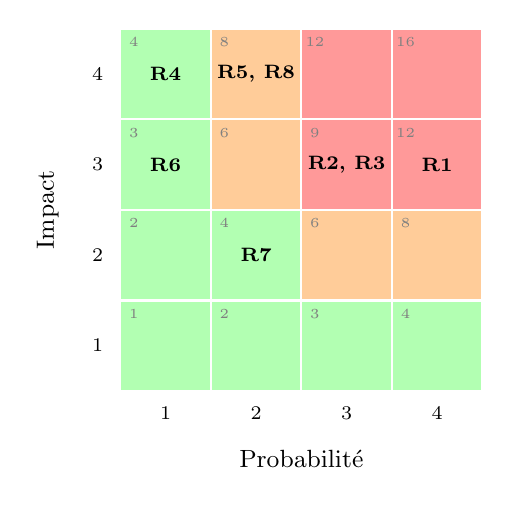
\begin{tikzpicture}[scale=1.15]
\foreach \p in {1,...,4}{
    \foreach \i in {1,...,4}{
        \pgfmathtruncatemacro{\s}{\p*\i}
        \ifnum\s>8 \def\coul{red!40}\else\ifnum\s>4 \def\coul{orange!40}\else\def\coul{green!30}\fi\fi
        \fill[\coul] (\p-1,\i-1) rectangle (\p,\i);
        \draw[white, thick] (\p-1,\i-1) rectangle (\p,\i);
        \node[font=\tiny, color=gray] at (\p-0.85,\i-0.15) {\s};
    }
}
\node[font=\scriptsize\bfseries] at (3.5,2.5) {R1};
\node[font=\scriptsize\bfseries] at (2.5,2.5) {R2, R3};
\node[font=\scriptsize\bfseries] at (1.5,3.5) {R5, R8};
\node[font=\scriptsize\bfseries] at (0.5,3.5) {R4};
\node[font=\scriptsize\bfseries] at (0.5,2.5) {R6};
\node[font=\scriptsize\bfseries] at (1.5,1.5) {R7};
\foreach \k in {1,...,4}{
    \node[font=\scriptsize] at (\k-0.5,-0.25) {\k};
    \node[font=\scriptsize] at (-0.25,\k-0.5) {\k};
}
\node[font=\small] at (2,-0.75) {Probabilité};
\node[font=\small, rotate=90] at (-0.8,2) {Impact};
\end{tikzpicture}
\end{center}
\vspace{-0.4em}
\begin{center}{\small\itshape Figure~3.1. Cartographie des risques
résiduels de LiZbiZ}\end{center}
\end{minipage}

\medskip

La cartographie se lit en trois temps~: les risques en zone rouge sont
traités en priorité~; les risques d'impact 4 restent sous surveillance même
en zone verte, car une erreur sur leur probabilité serait coûteuse~; et
l'écart entre risque inhérent et risque résiduel montre ce que les
contrôles apportent réellement.

\subsection{Traiter un risque}

Quatre options de traitement s'offrent à l'organisation~: \emph{réduire}
(ajouter ou renforcer des contrôles), \emph{transférer} (assurance,
sous-traitance, sans transférer la responsabilité), \emph{éviter} (renoncer
à l'activité) ou \emph{accepter} (dans les limites de l'appétence, par une
décision écrite).

\begin{boxprocedure}
\textbf{Le registre des risques.} Pour qu'un auditeur puisse s'appuyer sur la
cartographie, chaque ligne du registre indique~:
\begin{itemize}
    \item le risque, l'objectif menacé et son propriétaire~;
    \item la cotation inhérente, avec la justification de la probabilité et
          de l'impact~;
    \item les contrôles qui le réduisent, avec la date et le résultat de leur
          dernier test~;
    \item la cotation résiduelle et la décision de traitement~;
    \item pour un risque accepté, la décision écrite de l'instance
          compétente.
\end{itemize}
\end{boxprocedure}

\begin{boxmetier}{Responsable GRC}
\textbf{Tenir une cartographie utile}
\begin{enumerate}
    \item Faire approuver l'échelle de cotation et l'appétence par le
          conseil, avant toute cotation.
    \item Désigner un propriétaire par risque, au niveau de la direction.
    \item Ne réduire le risque résiduel que sur la base de contrôles testés.
    \item Mettre à jour la cartographie au moins une fois par an, et après
          tout incident majeur.
    \item Présenter au comité d'audit les risques en zone rouge et les
          décisions d'acceptation.
\end{enumerate}
\end{boxmetier}

\begin{boxscenario}{Opération SANAGA. Deux registres, deux échelles}
\textbf{Constatation.} La BANQUE SANAGA tient un registre des risques de
crédit et de marché, coté de 1 à 4, et la DSI un registre des risques
informatiques, coté de 1 à 5 avec d'autres critères d'impact.

\medskip
\textbf{Analyse} (confiance élevée). Le conseil ne peut pas comparer un
risque informatique à un risque de crédit, donc ne peut pas arbitrer. La
panne de mars~2026, cotée « 3 sur 5 » par la DSI, n'est jamais apparue
parmi les risques majeurs de la banque. Règle~: le risque informatique est
un risque de l'entreprise, à coter sur l'échelle commune.
\end{boxscenario}

% ============================================================================
\section{Les Risques de l'Audit}
\label{sec:c03-audit}
% ============================================================================

\subsection{Le modèle du risque d'audit}

L'auditeur court lui-même un risque~: conclure qu'une situation est
satisfaisante alors qu'elle ne l'est pas. La profession décompose ce
\termecle{risque d'audit}\index{risque d'audit} en trois éléments, que le
GUID~5100 de l'INTOSAI reprend pour l'audit des SI~\cite{intosai2019guid5100}.

\begin{boxdef}
\termecle{Risque inhérent}~(en audit)~: probabilité qu'une anomalie
significative existe, du fait de la nature même de l'activité ou du système.

\medskip
\termecle{Risque de contrôle}\index{risque de contrôle}~: probabilité que le
contrôle interne ne prévienne pas ou ne détecte pas cette anomalie.

\medskip
\termecle{Risque de détection}\index{risque de détection}~: probabilité que
les travaux de l'auditeur ne la détectent pas.
\end{boxdef}

Le modèle classique relie les trois~:
\[
    \text{RA} = \text{RI} \times \text{RC} \times \text{RD}.
\]
L'auditeur ne choisit ni le risque inhérent ni le risque de contrôle~: il
les évalue. Il choisit en revanche le risque de détection, en dimensionnant
ses tests, pour que le risque d'audit reste au niveau qu'il accepte.

\begin{boxscenario}{Opération LIZBIZ. Dimensionner les tests sur les stocks}
\textbf{Évaluation.} Risque inhérent élevé (stock de forte valeur, écart
déjà constaté), estimé à 0,9~; risque de contrôle élevé (contrôles de stock
inefficaces, Chapitre~\ref{chap:controle-interne}), estimé à 0,8. Risque
d'audit accepté~: 5~\%.

\medskip
\textbf{Calcul.} $\text{RD} = 0{,}05 / (0{,}9 \times 0{,}8) \approx 0{,}07$.

\medskip
\textbf{Analyse.} Le risque de détection doit être très faible~: AUDIX
CONSEIL ne peut pas se contenter de tester les contrôles. Il doit réaliser
des tests directs et étendus sur les données de stock
(Chapitre~\ref{chap:audit-applications}).
\end{boxscenario}

\begin{boiteRemarque}{Des probabilités vraiment mesurables~?}
Rarement. Les valeurs 0,9 ou 0,8 traduisent un jugement, pas une mesure.
Le modèle sert surtout à raisonner~: plus le risque inhérent et le risque de
contrôle sont élevés, plus les tests doivent être étendus. L'auditologie
propose d'aller plus loin en mesurant ce que l'auditeur sait réellement,
par $U$ et $H$, plutôt que de l'estimer (Chapitre~\ref{chap:conclure}).
\end{boiteRemarque}

\subsection{Un audit fondé sur les risques}

La cartographie des risques de l'organisation oriente le plan d'audit~:
on audite d'abord ce qui est le plus risqué et le moins bien connu. Le
Chapitre~\ref{chap:planifier} montrera comment passer de la cartographie au
plan d'audit.

% ============================================================================
\section{Les Référentiels du Risque}
\label{sec:c03-referentiels}
% ============================================================================

\begin{tableaucours}{L{2.8cm}L{4.4cm}L{5.0cm}}{%
    \tableauHeader{Référentiel} &
    \tableauHeader{Portée} &
    \tableauHeader{Apport}
}
ISO~31000:2018 & Tout risque, toute organisation~; non certifiable &
Principes, cadre organisationnel, processus~: contexte, appréciation
(identification, analyse, évaluation), traitement, surveillance,
communication~\cite{iso31000_2018} \\
COSO~ERM (2004, 2017) & Management des risques de l'entreprise & 2004~:
huit éléments, de l'environnement interne au pilotage~; 2017~: cinq
composantes, le risque intégré à la stratégie et à la
performance~\cite{coso2004ermfr,coso2017erm} \\
ISO/IEC~27005 & Risques liés à la sécurité de l'information & Processus
d'appréciation et de traitement, au service du SMSI de
l'ISO/IEC~27001~\cite{iso27005_2018} \\
\end{tableaucours}
\vspace{-0.8em}
\begin{center}{\small\itshape Tableau~3.3. Trois référentiels du
risque}\end{center}

\begin{boxinfo}
\textbf{Édition en vigueur.} Le dossier \texttt{Normes} du cours contient
l'ISO/IEC~27005 dans son édition de 2018. Une édition de 2022 l'a remplacée.
Avant de s'y référer dans un rapport, vérifiez toujours l'édition en
vigueur.
\end{boxinfo}

Ces référentiels convergent sur l'essentiel~: un risque se rattache à un
objectif, se cote sur une échelle commune, se traite selon une appétence
fixée par la gouvernance, et se surveille dans le temps. Les méthodes
d'analyse de risques (EBIOS Risk Manager, MEHARI, FAIR) relèvent de l'UE de
gestion des risques~; le présent cours en retient ce dont l'auditeur a
besoin.

\separateur

\begin{boxresume}
\textbf{Ce qu'il faut retenir de ce chapitre~:}
\begin{itemize}
    \item \textbf{Le risque est l'effet de l'incertitude sur les objectifs}~:
          on le rattache toujours à un objectif.
    \item \textbf{Inhérent, résiduel, appétence}~: le résiduel ne tient
          compte que des contrôles testés~; l'appétence est fixée par la
          gouvernance.
    \item \textbf{Risque et incertitude épistémique} ne se confondent pas~:
          le premier porte sur l'avenir de l'organisation, la seconde sur ce
          que l'on sait aujourd'hui.
    \item \textbf{Une échelle commune} (probabilité × impact) permet de
          comparer et d'arbitrer~; deux échelles rendent l'arbitrage
          impossible.
    \item \textbf{La cartographie} montre les priorités~; le registre en
          garde la justification.
    \item \textbf{Le risque d'audit} = inhérent × contrôle × détection~;
          l'auditeur agit sur le risque de détection en dimensionnant ses
          tests.
\end{itemize}
\end{boxresume}

\bigskip

\begin{boxexo}[title={\ding{45}\quad Exercice~3.1. Menace, vulnérabilité, impact \niveaubase}]
Pour chacun des risques R3, R5 et R8 du registre de LiZbiZ, identifiez la
menace, la vulnérabilité et l'objectif menacé, puis justifiez la cotation
d'impact au regard du Tableau~3.2.
\end{boxexo}

\begin{boxexo}[title={\ding{45}\quad Exercice~3.2. Après les contrôles \niveaumoyen}]
LiZbiZ met en place les contrôles proposés au Chapitre~\ref{chap:controle-interne}
(séparation des tâches, validation des ajustements, revue trimestrielle des
comptes). Les tests montrent qu'ils abaissent de deux niveaux la probabilité
de R1 et de R3, et d'un niveau celle de R2.
\begin{enumerate}[(a)]
    \item Recalculez les scores résiduels de R1, R2 et R3.
    \item Repositionnez ces trois risques dans la cartographie.
    \item Quels risques restent à traiter dans l'année~?
    \item Pourquoi faut-il attendre les tests avant de mettre à jour la
          cartographie~?
\end{enumerate}
\end{boxexo}

\begin{boxexo}[title={\ding{45}\quad Exercice~3.3. Une échelle commune pour la BANQUE SANAGA \niveauexpert}]
\begin{enumerate}[(a)]
    \item Proposez une échelle d'impact commune aux risques bancaires et
          informatiques, exprimée en FCFA et en durée d'interruption.
    \item Cotez sur cette échelle le risque « échec d'une migration du
          système central ».
    \item Évaluez le risque inhérent et le risque de contrôle d'un audit de
          la gestion des changements de la banque, et déduisez-en l'étendue
          des tests.
    \item Expliquez pourquoi une réponse \NEK{} sur l'existence d'un plan de
          retour arrière doit être signalée au conseil.
\end{enumerate}
\end{boxexo}

\bigskip

\begin{boxinfo}
\textbf{Transition.} Parmi les risques de LiZbiZ, trois sont intolérables et
supposent une intention~: ajuster le stock, payer des fournisseurs fictifs,
utiliser le compte d'un agent parti. Le Chapitre~\ref{chap:fraude} est
consacré à la fraude dans et par les systèmes d'information.
\end{boxinfo}

        % ============================================================================
% Fichier  : partie1/P01_C04_fraude.tex
% Titre    : La Fraude dans et par les Systèmes d'Information
% Auteur   : MINKA MI NGUIDJOÏ Thierry Emmanuel
% Version  : 1.0 -- octobre 2026
% ============================================================================
% Sources : COSO et ACFE, Guide de gestion du risque de fraude, synthèse
% (décembre 2016, dossier Normes) ; Cressey (1953) pour le triangle de la
% fraude ; COSO 2013 (principe 8) ; article A0 (axiome 4, interaction
% stratégique) et article A1 (usage stratégique de NEK). L'obligation de
% révélation du commissaire aux comptes (AUSCGIE) est décrite sans numéro
% d'article : à vérifier dans le texte.
% ============================================================================

\chapter{La Fraude dans et par les Systèmes d'Information}
\label{chap:fraude}
\chaptermark{La fraude et les SI}

\epigraph{%
    « L'erreur se cache par hasard.\\
    La fraude se cache exprès~: c'est ce qui la rend auditable. »%
}{Principe de l'auditeur}

\niveauChapitre{Intermédiaire}{%
    Maîtrise des Chapitres~\ref{chap:controle-interne} (séparation des
    tâches) et~\ref{chap:risque} (cartographie des risques)%
}

\begin{boxobjectifs}
\begin{itemize}
    \item Définir la fraude et la distinguer de l'erreur.
    \item Expliquer le triangle de la fraude et le relier à l'interaction
          stratégique entre auditeur et audité.
    \item Classer les schémas de fraude assistés par l'informatique et leurs
          signaux dans les données.
    \item Concevoir un dispositif de gestion du risque de fraude selon le
          guide du COSO et de l'ACFE.
    \item Reconnaître un usage stratégique de la réponse \NEK{}.
    \item Savoir quand l'audit doit s'arrêter et laisser place à
          l'enquête.
\end{itemize}
\end{boxobjectifs}

\bigskip

% ============================================================================
\section*{Question directrice : erreur ou fraude~?}
% ============================================================================

Au Chapitre~\ref{chap:risque}, trois risques intolérables de LiZbiZ
supposaient une intention~: ajuster le stock, payer des fournisseurs
fictifs, utiliser le compte d'un agent parti. Lorsque AUDIX CONSEIL
présente sa cartographie, le responsable informatique proteste~: « Ce sont
des erreurs de saisie, pas des fraudes. Nos agents sont honnêtes. »

Peut-être. Mais l'auditeur ne présume ni l'honnêteté ni la malhonnêteté~: il
cherche des faits. Ce chapitre définit la fraude
(section~\ref{sec:c04-definir}), explique pourquoi elle survient
(section~\ref{sec:c04-triangle}), décrit ses schémas dans les systèmes
d'information (section~\ref{sec:c04-schemas}), présente le dispositif qui la
prévient et la détecte (section~\ref{sec:c04-dispositif}), montre comment
la repérer dans les données et dans les réponses
(sections~\ref{sec:c04-donnees} et~\ref{sec:c04-strategie}), et fixe la
limite entre audit et enquête (section~\ref{sec:c04-enquete}).

\separateur

% ============================================================================
\section{Définir la Fraude}
\label{sec:c04-definir}
% ============================================================================

\begin{boxdef}
\termecle{Fraude}\index{fraude}~: acte \emph{intentionnel}, commis par une ou
plusieurs personnes de l'organisation ou extérieures à elle, qui recourt à
la tromperie pour obtenir un avantage indu ou causer un préjudice.

\medskip
\termecle{Erreur}\index{erreur}~: inexactitude \emph{non intentionnelle}
(faute de saisie, mauvaise interprétation d'une règle, panne).
\end{boxdef}

Ce qui distingue la fraude de l'erreur, c'est l'intention, et donc la
\emph{dissimulation}. Une erreur laisse des traces au hasard~; une fraude
efface les siennes, ou les place là où personne ne regarde. C'est pourquoi
la fraude obéit à des schémas, que l'auditeur peut connaître.

\begin{tableaucours}{L{3.6cm}L{4.4cm}L{4.2cm}}{%
    \tableauHeader{Famille} &
    \tableauHeader{Définition} &
    \tableauHeader{Exemple chez LiZbiZ}
}
Détournement d'actifs & Appropriation de biens ou de fonds de
l'organisation & Vol de marchandises masqué par un ajustement de stock \\
Corruption & Usage de sa fonction pour obtenir un avantage indu, souvent
avec un tiers & Commission versée par un transporteur pour être
retenu \\
Fraude à l'information financière & Présentation trompeuse des états
financiers & Stock surévalué pour améliorer le résultat \\
\end{tableaucours}
\vspace{-0.8em}
\begin{center}{\small\itshape Tableau~4.1. Trois familles de fraude
(classification usuelle de la profession)}\end{center}

% ============================================================================
\section{Pourquoi la Fraude Survient}
\label{sec:c04-triangle}
% ============================================================================

\subsection{Le triangle de la fraude}

Dans les années 1950, le criminologue Donald Cressey étudie des personnes
condamnées pour détournement de fonds~\cite{cressey1953}. Ses travaux ont
donné naissance au \termecle{triangle de la fraude}\index{triangle de la
fraude}~: la fraude survient lorsque trois conditions sont réunies.

\noindent\begin{minipage}{\linewidth}
\begin{center}
\begin{tikzpicture}[
    sommet/.style = {
        draw=CouleurPrimaire, fill=CouleurDef, rounded corners=4pt,
        text width=3.2cm, align=center, minimum height=1.0cm,
        font=\small\bfseries\color{CouleurPrimaire}
    }
]
\coordinate (A) at (0,3.0);
\coordinate (B) at (-3.0,0);
\coordinate (C) at (3.0,0);
\draw[very thick, color=CouleurAccent] (A) -- (B) -- (C) -- cycle;
\node[sommet] at (A) {Pression\\ \mdseries\footnotesize dette, objectifs intenables};
\node[sommet] at (B) {Opportunité\\ \mdseries\footnotesize contrôle faible, droits cumulés};
\node[sommet] at (C) {Rationalisation\\ \mdseries\footnotesize « je le rendrai », « on me doit »};
\node[font=\footnotesize\itshape, color=CouleurSecondaire] at (0,1.0) {Fraude};
\end{tikzpicture}
\end{center}
\vspace{-0.4em}
\begin{center}{\small\itshape Figure~4.1. Le triangle de la fraude, d'après
les travaux de Cressey}\end{center}
\end{minipage}

\medskip

L'auditeur et le contrôleur interne n'ont guère de prise sur la pression ni
sur la rationalisation. Ils agissent sur l'\textbf{opportunité}~: c'est
pourquoi la séparation des tâches et la revue des droits
(Chapitre~\ref{chap:controle-interne}) sont les premières défenses contre la
fraude. Des auteurs ont ajouté un quatrième élément, la \emph{capacité}~: la
position et les compétences qui permettent de passer à l'acte. Dans les
systèmes d'information, cette capacité est souvent technique~: un
administrateur peut faire ce que le contrôle interne interdit aux autres.

\subsection{Un jeu entre l'auditeur et l'audité}

L'auditologie pose que l'auditeur et l'audité poursuivent des intérêts
distincts, et que leurs actions se comprennent comme des coups dans un jeu
à information imparfaite (axiome~4~\cite{minka2026auditologie}). La fraude en
est le cas extrême~: le fraudeur sait ce que l'auditeur ignore, et cherche à
ce qu'il continue de l'ignorer. Deux conséquences pratiques en découlent.

\begin{enumerate}
    \item \textbf{L'audité adapte ses réponses à l'enjeu.} Une même personne
          ne répond pas de la même façon dans une auto-évaluation et dans un
          entretien formel (section~\ref{sec:c04-strategie}).
    \item \textbf{L'auditeur doit être imprévisible.} Un programme de tests
          connu d'avance indique au fraudeur où ne pas laisser de traces~:
          les échantillons, les dates et certains tests doivent rester
          inconnus de l'audité.
\end{enumerate}

% ============================================================================
\section{Les Schémas de Fraude Assistés par l'Informatique}
\label{sec:c04-schemas}
% ============================================================================

\begin{tableaucours}{L{2.9cm}L{3.2cm}L{3.0cm}L{3.1cm}}{%
    \tableauHeader{Schéma} &
    \tableauHeader{Vulnérabilité exploitée} &
    \tableauHeader{Contrôle préventif} &
    \tableauHeader{Signal dans les données}
}
Fournisseur fictif & Cumul création du fournisseur et paiement & Séparation
des tâches, validation des nouveaux fournisseurs & Coordonnées bancaires
partagées avec un salarié, absence d'adresse \\
Modification des coordonnées bancaires & Données de référence modifiables
sans validation & Double validation, journal des modifications &
Changement de RIB suivi d'un paiement dans les jours suivants \\
Fausse réception & Cumul commande et réception & Réception confirmée par
une personne distincte & Réception sans bon de transport, à l'heure de
fermeture \\
Ajustement de stock & Cumul réception et ajustement & Validation au-delà
d'un seuil & Ajustements concentrés en fin de mois, sans pièce \\
Fractionnement & Seuil de validation connu & Contrôle des cumuls par
fournisseur & Paiements juste sous le seuil, répétés \\
Compte dormant & Comptes d'agents partis non désactivés & Revue périodique
des comptes & Connexion après la date de départ \\
Abus d'administrateur & Droits techniques étendus, sans trace & Comptes
nominatifs, journalisation protégée & Opérations de gestion faites par un
compte d'administration \\
\end{tableaucours}
\vspace{-0.8em}
\begin{center}{\small\itshape Tableau~4.2. Schémas de fraude et
signaux}\end{center}

\begin{boxalert}
\textbf{Violation typique.} Laisser le responsable informatique, qui détient
tous les droits, administrer lui-même les journaux qui tracent ses propres
actions.

\smallskip
\textbf{Règle~:} les journaux des comptes d'administration sont conservés
hors de leur portée et examinés par une personne indépendante.
\end{boxalert}

% ============================================================================
\section{Le Dispositif Anti-Fraude}
\label{sec:c04-dispositif}
% ============================================================================

Le principe~8 du COSO~2013 demande de prendre en compte le risque de fraude
(Chapitre~\ref{chap:controle-interne}). Le COSO et l'Association of
Certified Fraud Examiners (\sigle{ACFE}) ont publié en 2016 un guide qui
décline cette exigence en un programme global de gestion du risque de
fraude~\cite{coso2016fraude}. Ses cinq principes sont alignés sur les cinq
composantes du contrôle interne.

\begin{tableaucours}{L{3.6cm}L{8.6cm}}{%
    \tableauHeader{Volet} &
    \tableauHeader{Contenu (reformulé)}
}
Gouvernance & Une politique écrite de gestion du risque de fraude, portée
par l'organe de gouvernance et la direction \\
Évaluation & Une évaluation régulière et complète du risque de fraude,
schéma par schéma \\
Activités de contrôle & Des contrôles préventifs et détectifs choisis pour
les schémas identifiés \\
Investigation et correction & Un dispositif de signalement et une approche
coordonnée des investigations et des mesures correctives \\
Pilotage & Des évaluations qui vérifient que les cinq volets fonctionnent,
et la communication des déficiences \\
\end{tableaucours}
\vspace{-0.8em}
\begin{center}{\small\itshape Tableau~4.3. Les cinq volets de la gestion du
risque de fraude (d'après COSO et ACFE, 2016)}\end{center}

\begin{boxmetier}{Contrôleur interne}
\textbf{Bâtir le programme anti-fraude de LiZbiZ}
\begin{enumerate}
    \item Faire adopter par le conseil une politique anti-fraude~: tolérance
          zéro, obligation de signaler, protection des lanceurs d'alerte.
    \item Dresser, schéma par schéma, la liste des fraudes possibles dans
          l'application intégrée (Tableau~4.2).
    \item Supprimer d'abord les opportunités~: cumuls de droits, comptes
          dormants, seuils connus et non surveillés.
    \item Mettre en place des contrôles détectifs automatiques sur les
          données, revus chaque mois.
    \item Ouvrir un canal de signalement confidentiel, hors de la
          hiérarchie directe.
\end{enumerate}
\end{boxmetier}

% ============================================================================
\section{Repérer la Fraude dans les Données}
\label{sec:c04-donnees}
% ============================================================================

L'informatique facilite la fraude, mais elle en garde la trace. L'auditeur
analyse l'ensemble des opérations, et non un échantillon, à la recherche des
signaux du Tableau~4.2~: doublons, valeurs juste sous un seuil, opérations
hors des heures de travail, coordonnées partagées entre un fournisseur et un
salarié. Le Chapitre~\ref{chap:audit-continu} présentera les outils de ces
analyses.

\begin{boxscenario}{Opération LIZBIZ. Ce que disent les données}
\textbf{Tests réalisés} par AUDIX CONSEIL sur les extractions de l'application
intégrée, pour 2025 et le premier trimestre~2026.

\medskip
\textbf{Constatation 1.} Le fournisseur « TRANSLOG SERVICES », créé en
mars~2025 par Mme~OWONA, a reçu 23~paiements de 4,9~millions FCFA chacun,
soit 112,7~millions FCFA. Le seuil de double validation est de 5~millions.
Ses coordonnées bancaires sont identiques à celles qu'un salarié a déclarées
pour sa paie.

\medskip
\textbf{Constatation 2.} À l'entrepôt de Douala, les ajustements négatifs de
stock saisis par M.~FOUDA s'élèvent à 148~millions FCFA, dont 71~\% le
dernier jour ouvré du mois. Aucun n'est appuyé par un procès-verbal
d'inventaire.

\medskip
\textbf{Constatation 3.} Sur l'écart de stock de 186~millions FCFA, 38~millions
ne peuvent être rattachés à aucune opération~: les extractions des autres
entrepôts sont incomplètes.

\medskip
\textbf{Analyse} (confiance moyenne). Les constatations 1 et 2 réunissent
les signaux de deux schémas~: fournisseur fictif avec fractionnement, et
ajustement de stock. Elles ne prouvent pas une fraude, car l'intention reste
à établir, mais elles imposent d'en informer le commanditaire. La
constatation 3 est cotée \NEK{}~: on ne sait pas, et il faut dire pourquoi.
\end{boxscenario}

% ============================================================================
\section{Repérer la Dissimulation dans les Réponses}
\label{sec:c04-strategie}
% ============================================================================

Le prologue l'a annoncé~: les réponses données en entretien formel ont
différé de celles de l'auto-évaluation. La réponse \NEK{} peut traduire une
ignorance sincère~; elle peut aussi servir à ne pas répondre. L'article
\emph{Modelling Epistemic Uncertainty in IS Audit} propose un indice, le
\termecle{SUI}\index{SUI (indice d'usage stratégique)} (\textit{Strategic Use
Index}), qui compare la distribution des \NEK{} entre questions à fort enjeu
et à faible enjeu, pour distinguer l'ignorance authentique de la
dissimulation~\cite{minka2026nek}. Le Chapitre~\ref{chap:incertitude} en
donnera la définition.

\begin{boxlecture}{Entrepôt de Douala}
Les mêmes dix questions sur la gestion du stock de Douala sont posées aux
mêmes deux responsables, d'abord en auto-évaluation écrite, puis en
entretien formel, après la découverte des ajustements.

\medskip
\begin{tableaucours}{L{3.6cm}ccccc}{%
    \tableauHeader{Contexte} &
    \tableauHeader{\OUI{}} & \tableauHeader{\NON{}} & \tableauHeader{\NEK{}} &
    \tableauHeader{$U$} & \tableauHeader{$H$ (bit)}
}
Auto-évaluation & 17 & 2 & 1 & 0,05 & 0,75 \\
Entretien formel & 9 & 3 & 8 & 0,40 & 1,46 \\
\end{tableaucours}

\medskip
\textbf{Constatation.} Le taux de \NEK{} passe de 5~\% à 40~\% lorsque
l'enjeu augmente, pour les mêmes personnes et les mêmes questions.

\medskip
\textbf{Analyse} (confiance faible à moyenne). Une ignorance sincère ne
devrait pas dépendre du contexte. Ce déplacement est un \emph{signal}
d'usage stratégique de \NEK{}, pas une preuve~: d'autres explications sont
possibles, comme la crainte de se tromper devant un auditeur. Il oriente
les tests vers les questions où \NEK{} a le plus augmenté.

\medskip
\hfill\lecture{0{,}45}{0{,}40}{1{,}46}
\end{boxlecture}

% ============================================================================
\section{De l'Audit à l'Enquête}
\label{sec:c04-enquete}
% ============================================================================

L'auditeur n'est ni un enquêteur ni un juge. Lorsque ses travaux révèlent des
indices sérieux de fraude, il ne poursuit pas seul.

\begin{boxprocedure}
\textbf{Conduite à tenir devant des indices de fraude.} Le papier de travail
de l'auditeur doit permettre d'établir qu'il a~:
\begin{itemize}
    \item conservé les extractions et les journaux utilisés, avec leur
          empreinte numérique, sans les modifier~;
    \item consigné les constatations séparément de leur analyse, sans
          qualification pénale («~fraude~», «~vol~»)~;
    \item informé le commanditaire désigné par la lettre de mission, par
          écrit, et non les personnes mises en cause~;
    \item suspendu les tests susceptibles d'alerter les personnes en cause,
          dans l'attente de la décision du commanditaire.
\end{itemize}
\end{boxprocedure}

La suite relève d'une enquête interne, d'un expert judiciaire ou de la
justice. Elle obéit aux règles de la preuve numérique~: chaîne de
conservation, intégrité, opposabilité. Le Chapitre~\ref{chap:audit-ia}
et le cours de Théorie et Pratique de l'Investigation Numérique y
reviennent.

\begin{boxmetier}{Commissaire aux comptes}
\textbf{Des indices de fraude dans l'audit légal}

Le commissaire aux comptes de LiZbiZ, informé des constatations d'AUDIX
CONSEIL, doit en apprécier l'effet sur les comptes~: stock surévalué,
charges fictives. Le droit OHADA des sociétés commerciales lui impose en
outre de révéler au ministère public les faits délictueux dont il a
connaissance dans l'exercice de sa mission~\cite{ohada2014auscgie}
(l'article est à vérifier dans le texte avant toute citation). Il ne peut
donc pas «~régler l'affaire en interne~».
\end{boxmetier}

\begin{boiteRemarque}{L'auditeur doit-il chercher la fraude~?}
Pas systématiquement~: la lettre de mission d'AUDIX CONSEIL l'exclut
(Chapitre~\ref{chap:audit-auditologie}). Mais il doit tenir compte du risque
de fraude dans la conception de ses tests, rester attentif aux signaux, et
ne jamais ignorer un indice qu'il a rencontré. Ne pas chercher n'est pas
fermer les yeux.
\end{boiteRemarque}

\separateur

\begin{boxresume}
\textbf{Ce qu'il faut retenir de ce chapitre~:}
\begin{itemize}
    \item \textbf{La fraude est intentionnelle et se dissimule}~; c'est ce
          qui la distingue de l'erreur et ce qui lui donne des schémas
          reconnaissables.
    \item \textbf{Le triangle de la fraude}~: pression, opportunité,
          rationalisation~; l'auditeur et le contrôleur agissent surtout sur
          l'opportunité.
    \item \textbf{Les schémas assistés par l'informatique} exploitent des
          cumuls de droits, des données de référence non protégées, des seuils
          connus et des comptes dormants~; chacun laisse un signal dans les
          données.
    \item \textbf{Un programme anti-fraude} a cinq volets~: gouvernance,
          évaluation, contrôles, investigation et correction, pilotage.
    \item \textbf{La réponse \NEK{}} peut être stratégique~: un taux de \NEK{}
          qui dépend de l'enjeu est un signal, pas une preuve.
    \item \textbf{Devant des indices}, l'auditeur conserve les preuves,
          informe le commanditaire et laisse la place à l'enquête.
\end{itemize}
\end{boxresume}

\bigskip

\begin{boxexo}[title={\ding{45}\quad Exercice~4.1. Erreur ou fraude~? \niveaubase}]
Pour chacune des situations suivantes, indiquez s'il s'agit plutôt d'une
erreur ou d'un signal de fraude, et le test qui permettrait de trancher.
\begin{enumerate}[(a)]
    \item Une facture est saisie deux fois, avec deux numéros différents.
    \item Les coordonnées bancaires d'un transporteur sont modifiées, puis
          rétablies trois jours plus tard, après un paiement.
    \item Un ajustement de stock positif compense exactement un ajustement
          négatif de la veille.
    \item Une commande est passée un dimanche par un compte d'administration.
\end{enumerate}
\end{boxexo}

\begin{boxexo}[title={\ding{45}\quad Exercice~4.2. Le triangle de TRANSLOG SERVICES \niveaumoyen}]
Reprenez la constatation 1 de la section~\ref{sec:c04-donnees}.
\begin{enumerate}[(a)]
    \item Identifiez l'élément du triangle de la fraude sur lequel LiZbiZ peut
          agir, et les contrôles correspondants.
    \item Rédigez la constatation de façon factuelle, sans qualification
          pénale.
    \item Proposez deux tests complémentaires qui confirmeraient ou
          infirmeraient le caractère fictif du fournisseur.
\end{enumerate}
\end{boxexo}

\begin{boxexo}[title={\ding{45}\quad Exercice~4.3. Un usage stratégique de NEK~? \niveauexpert}]
Reprenez la lecture de l'entrepôt de Douala (section~\ref{sec:c04-strategie}).
\begin{enumerate}[(a)]
    \item Recalculez $\mu$, $U$ et $H$ pour l'auto-évaluation et pour
          l'entretien formel.
    \item Proposez deux explications du déplacement des réponses, l'une
          sincère, l'autre stratégique.
    \item Concevez un protocole de recueil qui permettrait de départager ces
          deux explications.
    \item Rédigez la note que le chef de mission adresse au commanditaire, en
          respectant la conduite à tenir de la section~\ref{sec:c04-enquete}.
\end{enumerate}
\end{boxexo}

\bigskip

\begin{boxinfo}
\textbf{Transition.} La Partie~\ref{part:fondements} a posé ce que l'auditeur
doit savoir~: ce qu'est un audit, le contrôle interne, le risque et la
fraude. La Partie~\ref{part:methode} enseigne comment conduire la mission.
Le Chapitre~\ref{chap:mission} en présente les principes et le cycle.
\end{boxinfo}


    % ======================================================================
    % PARTIE 2 — MÉTHODE DE LA MISSION D'AUDIT
    % Standards de référence : ISO 19011, normes IIA ; articles A0 (hal-05701007) et A1 (hal-05701270).
    % Niveau : fondamental à intermédiaire
    % ======================================================================
    \part{Méthode de la Mission d'Audit}
    \label{part:methode}

        % ============================================================================
% Fichier  : partie2/P02_C05_mission_principes_cycle.tex
% Titre    : La Mission d'Audit : Principes et Cycle
% Auteur   : MINKA MI NGUIDJOÏ Thierry Emmanuel
% Version  : 1.0 -- octobre 2026
% ============================================================================
% Sources : ISO 19011:2018 (sept principes ; l'édition 2011 du cours Audit_SI
% en comptait six) ; Normes mondiales d'audit interne de l'IIA (2024),
% domaine III (charte, rattachement au conseil) ; boîte à outils O0 à O9 du
% cours Audit_SI de l'auteur, mise en cohérence avec les articles A0 et A1
% (gabarit canonique, OUI/NON/NEK, µ, U, H).
% ============================================================================

\chapter{La Mission d'Audit : Principes et Cycle}
\label{chap:mission}

\epigraph{%
    « Une mission d'audit se gagne avant le terrain\\
    et se perd après le rapport. »%
}{Adage des chefs de mission}

\niveauChapitre{Fondamental}{%
    Maîtrise du Chapitre~\ref{chap:audit-auditologie} (audit, assurance,
    axiomes de l'auditologie)%
}

\begin{boxobjectifs}
\begin{itemize}
    \item Énoncer les sept principes de l'audit selon l'ISO~19011:2018.
    \item Expliquer le rôle de la charte d'audit et de la lettre de mission.
    \item Décrire les cinq phases de la mission, leurs entrées et leurs
          livrables.
    \item Situer les dix outils de la méthode (O0 à O9) dans le cycle.
    \item Organiser le contradictoire et le relier à l'opposabilité des
          conclusions (axiome~6).
    \item Montrer comment le contradictoire réduit l'incertitude de la
          mission.
\end{itemize}
\end{boxobjectifs}

\bigskip

% ============================================================================
\section*{Question directrice : comment ne pas refaire la première mission~?}
% ============================================================================

La première mission de LiZbiZ (Chapitre~\ref{chap:prologue}) a échoué
faute de mandat, de critères et de preuves. Pour la seconde, le cabinet
AUDIX CONSEIL n'improvise rien~: M.~BEYALA ouvre la mission par une réunion
avec le directeur général, remet une lettre de mission, annonce un
calendrier en cinq phases et prévient que chaque constat sera discuté avec
les audités avant d'être écrit.

Ce chapitre présente cette organisation. Il pose les principes qui guident
l'auditeur (section~\ref{sec:c05-principes}), les documents qui fondent sa
mission (section~\ref{sec:c05-charte}), le cycle de la mission
(section~\ref{sec:c05-cycle}), les outils qui l'outillent
(section~\ref{sec:c05-outils}) et le contradictoire qui la rend opposable
(section~\ref{sec:c05-contradictoire}). Les Chapitres~\ref{chap:planifier}
à~\ref{chap:conclure} détaillent ensuite chaque phase.

\separateur

% ============================================================================
\section{Les Principes de l'Audit}
\label{sec:c05-principes}
% ============================================================================

L'ISO~19011 donne des lignes directrices pour l'audit des systèmes de
management. Ses principes valent pour tout audit, et en particulier pour
l'audit des SI~\cite{iso19011_2018}.

\begin{tableaucours}{L{3.4cm}L{4.4cm}L{4.4cm}}{%
    \tableauHeader{Principe} &
    \tableauHeader{Sens (reformulé)} &
    \tableauHeader{Chez LiZbiZ}
}
Intégrité & Honnêteté, diligence, responsabilité & Ne pas taire un constat
qui gêne la direction \\
Présentation impartiale & Rendre compte avec exactitude et fidélité &
Ne pas grossir un risque mineur, ne pas minimiser un risque majeur \\
Conscience professionnelle & Diligence et jugement proportionnés à
l'enjeu & Ne pas lancer un test de charge à l'heure de pointe \\
Confidentialité & Protéger l'information obtenue & Ne pas divulguer les
failles constatées \\
Indépendance & Impartialité, absence de conflit d'intérêts & Ne pas auditer
l'application qu'on a conçue \\
Approche fondée sur la preuve & Des conclusions vérifiables, appuyées sur
un échantillon adapté & Une capture, une extraction, pas un ouï-dire \\
Approche par les risques & Concentrer l'effort sur ce qui compte pour les
objectifs & Commencer par les risques intolérables du registre \\
\end{tableaucours}
\vspace{-0.8em}
\begin{center}{\small\itshape Tableau~5.1. Les sept principes de l'audit
selon l'ISO~19011:2018 (notre reformulation)}\end{center}

\begin{boxinfo}
\textbf{Six ou sept principes~?} L'édition de 2011 de l'ISO~19011 en
comptait six. L'édition de 2018, en vigueur, ajoute l'\emph{approche par
les risques}. Un support qui annonce « six principes » se réfère à
l'ancienne édition.
\end{boxinfo}

Deux de ces principes trouvent un fondement dans l'auditologie. L'approche
fondée sur la preuve découle de l'axiome d'opposabilité~: une conclusion
doit pouvoir être défendue devant un tiers. L'indépendance, on l'a vu au
Chapitre~\ref{chap:audit-auditologie}, se déduit de l'interaction
stratégique et de l'opposabilité~\cite{minka2026auditologie}.

% ============================================================================
\section{Charte d'Audit et Lettre de Mission}
\label{sec:c05-charte}
% ============================================================================

\subsection{La charte d'audit}

\begin{boxdef}
\termecle{Charte d'audit}\index{charte d'audit}~: document approuvé par
l'organe de gouvernance, qui fixe la mission de l'audit, ses pouvoirs (accès
aux personnes, aux documents et aux systèmes), son rattachement, son
indépendance et ses responsabilités.
\end{boxdef}

Les Normes mondiales d'audit interne de l'IIA placent sous la
responsabilité du conseil la supervision de la fonction d'audit, son mandat
et les moyens de son indépendance~\cite{iia2024gias}. La charte en est
l'instrument~: sans elle, l'auditeur dépend du bon vouloir de ceux qu'il
audite.

\subsection{La lettre de mission}

Chaque mission est ensuite fondée sur une \termecle{lettre de
mission}\index{lettre de mission}, ou des termes de référence, qui précise
ce qu'elle doit démontrer. Le Chapitre~\ref{chap:audit-auditologie} en a
donné un exemple pour LiZbiZ~; le Chapitre~\ref{chap:planifier} en détaille
le contenu.

\begin{boxalert}
\textbf{Violation typique.} Le plan d'audit interne d'une entreprise est
approuvé par le directeur général, dont relèvent les directions auditées.

\smallskip
\textbf{Règle~:} le plan d'audit et les moyens de l'audit sont approuvés par
l'organe de gouvernance (conseil, comité d'audit), et non par la direction
auditée.
\end{boxalert}

% ============================================================================
\section{Le Cycle de la Mission}
\label{sec:c05-cycle}
% ============================================================================

\subsection{Cinq phases}

\noindent\begin{minipage}{\linewidth}
\begin{center}
\begin{tikzpicture}[
    phase/.style = {
        draw=CouleurPrimaire, fill=CouleurPrimaire, rounded corners=4pt,
        text width=2.1cm, minimum height=1.1cm, align=center,
        font=\scriptsize\bfseries\color{white}
    },
    livr/.style = {
        draw=CouleurBordDef, fill=CouleurDef, rounded corners=3pt,
        text width=2.0cm, align=center, font=\scriptsize\color{CouleurPrimaire}
    },
    fleche/.style = {-{Stealth[length=5pt]}, thick, color=CouleurSecondaire}
]
\foreach \n/\t/\l [count=\i] in {
    0/Préparation/Termes de référence,
    1/Planification/Plan d'audit,
    2/Exécution/Papiers de travail,
    3/Rapport/Rapport contradictoire,
    4/Suivi/Tableau de suivi} {
    \node[phase] (p\i) at (2.55*\i, 0) {Phase~\n\\ \t};
    \node[livr, below=0.35cm of p\i] {\l};
}
\foreach \i [evaluate=\i as \j using int(\i+1)] in {1,...,4}
    \draw[fleche] (p\i) -- (p\j);
\draw[fleche] (p5.north) to[out=150, in=30] node[above, font=\scriptsize\itshape]
    {mission suivante} (p1.north);
\end{tikzpicture}
\end{center}
\vspace{-0.4em}
\begin{center}{\small\itshape Figure~5.1. Les cinq phases de la mission et
leurs livrables}\end{center}
\end{minipage}

\medskip

\begin{tableaucours}{L{2.6cm}L{4.8cm}L{4.8cm}}{%
    \tableauHeader{Phase} &
    \tableauHeader{Activités principales} &
    \tableauHeader{Chapitre}
}
0. Préparation & Mandat, termes de référence, documents sollicités,
équipe & Chapitre~\ref{chap:planifier} \\
1. Planification & Prise de connaissance, cartographie préliminaire des
risques, décomposition de l'espace d'audit, plan d'audit &
Chapitres~\ref{chap:planifier} et~\ref{chap:decomposition} \\
2. Exécution & Entretiens, tests, cotation \OUI{}~/ \NON{}~/ \NEK{}, papiers
de travail & Chapitre~\ref{chap:preuve} \\
3. Rapport & Calcul de $\mu$, $U$, $H$, observations, contradictoire,
rapport & Chapitre~\ref{chap:conclure} \\
4. Suivi & Suivi des recommandations, préparation du cycle suivant &
Chapitre~\ref{chap:conclure} \\
\end{tableaucours}
\vspace{-0.8em}
\begin{center}{\small\itshape Tableau~5.2. Les phases de la mission}\end{center}

Le cycle ne se referme pas sur lui-même~: le suivi d'une mission prépare la
suivante. C'est la dimension temporelle de l'audit, que l'auditologie pose
en axiome~: le système audité évolue, et son état à la mission suivante
dépend des interventions déclenchées par la précédente (axiome~5,
\emph{individuation temporelle}~\cite{minka2026auditologie}).

\subsection{La mission d'AUDIX CONSEIL chez LiZbiZ}

\begin{boxscenario}{Opération LIZBIZ. Le calendrier de la seconde mission}
\begin{tableaucours}{L{3.0cm}L{2.6cm}L{6.2cm}}{%
    \tableauHeader{Phase} &
    \tableauHeader{Dates (2026)} &
    \tableauHeader{Faits marquants}
}
0. Préparation & 4 -- 8 mai & Lettre de mission signée~; 21 documents
sollicités \\
1. Planification & 11 -- 22 mai & Prise de connaissance des quatre centres
de données~; décomposition du domaine D~; plan d'audit validé par le
directeur général \\
2. Exécution & 25 mai -- 26 juin & Entretiens, extractions, tests sur
quatre agences \\
3. Rapport & 29 juin -- 17 juillet & Réunion de restitution, réponses
écrites des audités, rapport final \\
4. Suivi & À partir de janvier~2027 & Revue de la mise en œuvre des
recommandations \\
\end{tableaucours}

\medskip
\textbf{Analyse} (confiance élevée). Le calendrier réserve trois semaines
au rapport et au contradictoire~: c'est le temps nécessaire pour que les
conclusions soient discutées, et donc opposables.
\end{boxscenario}

% ============================================================================
\section{La Boîte à Outils de la Méthode}
\label{sec:c05-outils}
% ============================================================================

La méthode du cours est outillée~: à chaque phase correspondent un ou
plusieurs instruments, numérotés de O0 à O9. Ils seront construits au fil
des chapitres et rassemblés en annexe.

\begin{tableaucours}{cL{3.6cm}L{2.4cm}L{5.4cm}}{%
    \tableauHeader{Outil} &
    \tableauHeader{Nom} &
    \tableauHeader{Phase} &
    \tableauHeader{Usage}
}
O0 & Aide-mémoire du cycle & Toutes & Entrées, activités et livrables de
chaque phase \\
O1 & Fiche technique de la mission & 0 & Présentation de la mission~:
objectifs, acteurs, référentiels \\
O2 & Termes de référence & 0 & Objectifs, périmètre, équipe, livrables,
calendrier \\
O3 & Liste des documents sollicités & 0 & Documents attendus, priorité,
interlocuteur~; un document essentiel absent est coté \NEK{} \\
O4 & Classeur d'aide à l'audit & 1 à 3 & Décomposition selon le gabarit
canonique, fiches d'assertion, cotation \OUI{}~/ \NON{}~/ \NEK{}, calcul de
$\mu$, $U$ et $H$ par domaine \\
O5 & Guide d'entretien & 2 & Questions issues des fiches d'assertion,
classées par interlocuteur \\
O6 & Plan d'audit & 1 & Contexte, périmètre, risques, programme de
travail, calendrier \\
O7 & Plan de tests & 2 & Tests codifiés, preuves attendues, références des
papiers de travail \\
O8 & Projets d'observation & 3 & Observations en sept éléments, soumises
au contradictoire \\
O9 & Suivi des documents & 2 & Mise à jour, sur le terrain, de la liste O3 \\
\end{tableaucours}
\vspace{-0.8em}
\begin{center}{\small\itshape Tableau~5.3. Les outils O0 à O9}\end{center}

L'outil central est le classeur~O4~: il porte la décomposition de l'espace
d'audit (Chapitre~\ref{chap:decomposition}), la cotation des réponses
(Chapitre~\ref{chap:preuve}) et les trois mesures de chaque domaine
(Chapitre~\ref{chap:conclure}).

\begin{boxmetier}{Auditeur SI}
\textbf{Ouvrir une mission}
\begin{enumerate}
    \item Vérifier que la charte ou la lettre de mission donne l'accès aux
          personnes, aux documents et aux systèmes nécessaires.
    \item Tenir une réunion d'ouverture avec le commanditaire et les
          principaux audités~: objectifs, périmètre, calendrier, règles du
          contradictoire.
    \item Annoncer que la réponse \NEK{} est admise et documentée, et qu'un
          document non remis sera coté comme tel.
    \item Remettre la liste des documents sollicités (O3) avec une date de
          remise.
    \item Consigner la réunion dans un compte rendu, premier papier de
          travail de la mission.
\end{enumerate}
\end{boxmetier}

% ============================================================================
\section{Le Contradictoire}
\label{sec:c05-contradictoire}
% ============================================================================

\subsection{Pourquoi le contradictoire~?}

\begin{boxdef}
\termecle{Contradictoire}\index{contradictoire}~: principe selon lequel
l'audité prend connaissance des constats qui le concernent et peut y
répondre, avant que le rapport ne soit définitif~; ses réponses sont
consignées et, le cas échéant, reproduites dans le rapport.
\end{boxdef}

Le contradictoire n'est pas une politesse. Il remplit trois fonctions~:
\begin{enumerate}
    \item \textbf{Corriger les erreurs} de l'auditeur, qui a pu mal
          comprendre un processus ou manquer une pièce.
    \item \textbf{Rendre les conclusions opposables}~: un constat discuté et
          maintenu est plus difficile à contester qu'un constat découvert
          dans le rapport (axiome~6).
    \item \textbf{Réduire l'incertitude}~: l'audité apporte souvent, au
          moment du contradictoire, l'information qui manquait.
\end{enumerate}

\subsection{Le contradictoire réduit l'incertitude}

\begin{boxlecture}{Domaine B, avant et après la restitution}
Douze questions du domaine~B (gestion des sauvegardes) sont cotées avant la
réunion de restitution, puis après, lorsque le responsable informatique
remet les journaux de sauvegarde qu'il n'avait pas fournis.

\medskip
\begin{tableaucours}{L{3.8cm}ccccc}{%
    \tableauHeader{Moment} &
    \tableauHeader{\OUI{}} & \tableauHeader{\NON{}} & \tableauHeader{\NEK{}} &
    \tableauHeader{$U$} & \tableauHeader{$H$ (bit)}
}
Avant la restitution & 6 & 2 & 4 & 0,33 & 1,46 \\
Après la restitution & 8 & 3 & 1 & 0,08 & 1,19 \\
\end{tableaucours}

\medskip
\textbf{Constatation.} Le taux d'incertitude passe de 0,33 à 0,08~: trois
\NEK{} sont levés, deux en \OUI{}, un en \NON{}.

\medskip
\textbf{Analyse} (confiance élevée). Le contradictoire a surtout réduit
l'ignorance. L'entropie baisse moins, parce que les réponses restent
partagées entre \OUI{} et \NON{}~: le domaine est désormais mieux connu,
et l'on sait où il est défaillant. Sans restitution, le rapport aurait
conclu sur un tiers de réponses inconnues.

\medskip
\hfill\lecture{0{,}67}{0{,}08}{1{,}19}
\end{boxlecture}

\begin{boxprocedure}
\textbf{La trace du contradictoire.} Pour qu'un constat soit opposable, le
dossier de la mission contient~:
\begin{itemize}
    \item le projet d'observation transmis à l'audité, daté~;
    \item la réponse écrite de l'audité, ou le compte rendu de la réunion de
          restitution signé des participants~;
    \item la position finale de l'auditeur~: constat maintenu, modifié ou
          retiré, et pourquoi~;
    \item les pièces nouvelles remises au moment du contradictoire, avec leur
          date de remise.
\end{itemize}
\end{boxprocedure}

\begin{boxalert}
\textbf{Violation typique.} Accepter, au contradictoire, une affirmation de
l'audité («~les sauvegardes sont testées chaque mois~») et changer un
\NON{} en \OUI{} sans pièce.

\smallskip
\textbf{Règle~:} au contradictoire, une affirmation sans pièce peut lever un
malentendu, jamais remplacer une preuve. Elle transforme au mieux un \NON{}
en \NEK{}, en attendant la pièce.
\end{boxalert}

\begin{boxmetier}{RSSI}
\textbf{Se préparer à être audité}
\begin{enumerate}
    \item Remettre les documents sollicités dans les délais~: un document
          non remis sera coté \NEK{}, et signalé comme tel.
    \item Désigner un interlocuteur unique pour l'équipe d'audit.
    \item Répondre par écrit aux projets d'observation, pièce à l'appui.
    \item Proposer, pour chaque recommandation acceptée, un responsable et
          une échéance.
\end{enumerate}
\end{boxmetier}

\separateur

\begin{boxresume}
\textbf{Ce qu'il faut retenir de ce chapitre~:}
\begin{itemize}
    \item \textbf{Sept principes} guident l'auditeur selon l'ISO~19011:2018,
          dont l'approche fondée sur la preuve et l'approche par les risques.
    \item \textbf{La charte d'audit} fonde les pouvoirs et l'indépendance de
          l'audit~; elle est approuvée par l'organe de gouvernance.
    \item \textbf{Cinq phases}~: préparation, planification, exécution,
          rapport, suivi~; le suivi prépare la mission suivante.
    \item \textbf{Dix outils} (O0 à O9) outillent le cycle~; le classeur O4
          porte la décomposition, la cotation et les mesures.
    \item \textbf{Le contradictoire} corrige, rend opposable et réduit
          l'incertitude~; une affirmation sans pièce ne remplace jamais une
          preuve.
\end{itemize}
\end{boxresume}

\bigskip

\begin{boxexo}[title={\ding{45}\quad Exercice~5.1. Quel principe~? \niveaubase}]
Indiquez le principe de l'ISO~19011 que chacune des situations suivantes
méconnaît.
\begin{enumerate}[(a)]
    \item Un auditeur évoque, lors d'un dîner, les failles du système de
          paiement de la BANQUE SANAGA.
    \item Un rapport passe sous silence un constat qui met en cause le
          directeur général.
    \item Un auditeur consacre autant de temps aux imprimantes qu'aux
          comptes à privilèges.
    \item Un constat repose sur ce qu'un agent a « entendu dire ».
\end{enumerate}
\end{boxexo}

\begin{boxexo}[title={\ding{45}\quad Exercice~5.2. La charte d'audit de LiZbiZ \niveaumoyen}]
LiZbiZ veut créer une fonction d'audit interne.
\begin{enumerate}[(a)]
    \item Rédigez les cinq rubriques principales de sa charte d'audit.
    \item À qui la directrice de l'audit doit-elle être rattachée, et
          pourquoi~?
    \item Quels pouvoirs d'accès faut-il prévoir pour auditer l'application
          intégrée et les quatre centres de données~?
\end{enumerate}
\end{boxexo}

\begin{boxexo}[title={\ding{45}\quad Exercice~5.3. Le contradictoire à la BANQUE SANAGA \niveauexpert}]
Mme~EKAMBI présente à la DSI un projet d'observation~: aucun test de retour
arrière n'a été réalisé avant la bascule de mars~2026. La DSI répond que des
tests ont eu lieu, mais que leurs comptes rendus ont été perdus.
\begin{enumerate}[(a)]
    \item Quelle cotation retenir pour ce contrôle, avant et après la
          réponse de la DSI~? Justifiez.
    \item Que doit contenir le dossier pour que le constat final soit
          opposable~?
    \item Rédigez la position finale de l'auditrice.
    \item En quoi cette situation illustre-t-elle la différence entre réduire
          l'incertitude et lever un constat~?
\end{enumerate}
\end{boxexo}

\bigskip

\begin{boxinfo}
\textbf{Transition.} La mission commence avant le terrain. Le
Chapitre~\ref{chap:planifier} détaille la préparation et la planification~:
termes de référence, documents sollicités, prise de connaissance du système
d'information et plan d'audit.
\end{boxinfo}

        % ============================================================================
% Fichier  : partie2/P02_C06_preparer_planifier.tex
% Titre    : Préparer et Planifier la Mission
% Auteur   : MINKA MI NGUIDJOÏ Thierry Emmanuel
% Version  : 1.0 -- octobre 2026
% ============================================================================
% Sources : cours Audit_SI de l'auteur (travaux préparatoires, documents à
% solliciter, strates documentaires, lecture du SI en couches, entretiens par
% niveau décisionnel), mis en cohérence avec les articles A0 et A1 (cotation
% NEK, mesures µ, U, H) ; ordres de grandeur d'échantillonnage repris du
% cours GCI (chapitre 11), indicatifs et non normatifs.
% ============================================================================

\chapter{Préparer et Planifier la Mission}
\label{chap:planifier}

\epigraph{%
    « Le temps passé à préparer\\
    se reprend sur le terrain, au double. »%
}{Adage des chefs de mission}

\niveauChapitre{Fondamental}{%
    Maîtrise des Chapitres~\ref{chap:risque} (cartographie) et~\ref{chap:mission}
    (cycle, outils O0 à O9)%
}

\begin{boxobjectifs}
\begin{itemize}
    \item Distinguer les travaux préparatoires de la planification.
    \item Rédiger les termes de référence d'une mission en répondant à quatre
          questions~: quand, comment, par qui, avec quoi.
    \item Établir la liste des documents sollicités, et coter \NEK{} ou
          \NON{} un document absent selon le cas.
    \item Prendre connaissance d'un système d'information par couches, par
          strates documentaires et par niveaux d'interlocuteurs.
    \item Évaluer a priori le contrôle interne et produire la cartographie
          préliminaire des risques.
    \item Dimensionner les échantillons et rédiger le plan d'audit.
\end{itemize}
\end{boxobjectifs}

\bigskip

% ============================================================================
\section*{Question directrice : que faut-il savoir avant d'auditer~?}
% ============================================================================

AUDIX CONSEIL dispose de huit semaines pour auditer LiZbiZ~: quatre
centres de données, douze agences, une application intégrée, des milliers
de comptes et de mouvements de stock. Impossible de tout voir. M.~BEYALA
consacre donc les deux premières semaines à décider \emph{quoi} auditer,
\emph{où}, \emph{avec qui} et \emph{comment}, avant le moindre test.

Ce chapitre décrit ce travail. Il sépare la préparation de la
planification (section~\ref{sec:c06-deux-phases}), présente les termes de
référence (section~\ref{sec:c06-tdr}) et les documents sollicités
(section~\ref{sec:c06-documents}), puis la prise de connaissance
(section~\ref{sec:c06-connaissance}), l'évaluation a priori et la
cartographie préliminaire (section~\ref{sec:c06-risques}), et enfin le plan
d'audit (section~\ref{sec:c06-plan}).

\separateur

% ============================================================================
\section{Préparer, puis Planifier}
\label{sec:c06-deux-phases}
% ============================================================================

\begin{boxdef}
\termecle{Travaux préparatoires}\index{travaux préparatoires} (phase~0)~:
diligences qui conduisent à la lettre de mission et à la constitution de
l'équipe~: analyse préalable des risques, termes de référence, ressources.

\medskip
\termecle{Planification}\index{planification} (phase~1)~: diligences qui
préparent le terrain à partir de la lettre de mission~: prise de
connaissance, cartographie préliminaire des risques, décomposition de
l'espace d'audit, plan d'audit.
\end{boxdef}

On confond souvent les deux, parce que, du point de vue du contrat, la
mission commence à la signature de la lettre de mission. Du point de vue de
la démarche, la préparation \emph{produit} la lettre de mission~; la
planification l'\emph{exploite}. Les acteurs diffèrent aussi~: la
préparation associe étroitement le commanditaire, la planification
mobilise surtout l'équipe d'audit.

% ============================================================================
\section{Les Termes de Référence}
\label{sec:c06-tdr}
% ============================================================================

\subsection{Quatre questions}

Les termes de référence (outil~O2) répondent à quatre questions, qui
déterminent le coût et la faisabilité de la mission.

\begin{tableaucours}{L{2.4cm}L{5.0cm}L{4.8cm}}{%
    \tableauHeader{Question} &
    \tableauHeader{Contenu} &
    \tableauHeader{Chez LiZbiZ}
}
Quand~? & Période auditée, durée de la mission & Janvier à avril~2026~;
huit semaines \\
Comment~? & Type d'audit, objectifs, périmètre, référentiels, points
d'attention du commanditaire & Audit d'application (stocks) et audit de
sécurité (contrôle d'accès)~; COSO, ISO/IEC~27002 \\
Par qui~? & Profils requis, auditeurs internes ou externes, absence de
conflit d'intérêts & Un chef de mission, un auditeur réseau et sécurité, un
auditeur données (SQL) \\
Avec quoi~? & Moyens matériels, accès, budget & Accès en lecture à la base,
outil d'analyse de données, déplacements à Garoua et Bafoussam \\
\end{tableaucours}
\vspace{-0.8em}
\begin{center}{\small\itshape Tableau~6.1. Les quatre questions des termes
de référence}\end{center}

\subsection{Les livrables de la préparation}

À l'issue de la phase~0, le dossier de la mission contient les termes de
référence, la fiche technique (O1), la lettre de mission signée, et selon
le cas le contrat, l'engagement de confidentialité, la déclaration d'absence
de conflit d'intérêts de chaque auditeur et les autorisations d'accès aux
sites.

% ============================================================================
\section{Les Documents Sollicités}
\label{sec:c06-documents}
% ============================================================================

\subsection{Trois strates de documents}

La liste des documents sollicités (outil~O3) se construit selon le type
d'audit. Les documents n'ont pas tous la même valeur~: on les classe en trois
strates.

\begin{tableaucours}{L{2.4cm}L{3.8cm}L{3.0cm}L{3.0cm}}{%
    \tableauHeader{Strate} &
    \tableauHeader{Exemples} &
    \tableauHeader{Ce qu'ils révèlent} &
    \tableauHeader{Si absents}
}
1. Stratégique & Schéma directeur, politique de sécurité, plan de
continuité, rapports d'audit précédents & L'engagement de la direction &
Gouvernance informelle, recommandations non suivies \\
2. Organisationnelle & Organigramme de la DSI, cartographie des
applications et des interfaces, matrice des droits & Qui fait quoi &
Responsabilités floues, cumuls de fonctions \\
3. Opérationnelle & Journaux d'incidents, de sauvegardes, de traitements~;
inventaires & Ce qui se fait réellement & Impossible de distinguer le
déclaré du réel \\
\end{tableaucours}
\vspace{-0.8em}
\begin{center}{\small\itshape Tableau~6.2. Les strates documentaires}\end{center}

La confrontation des strates est en soi une source de constats~: une
politique de sécurité (strate~1) qui exige une revue trimestrielle des
droits, sans aucune trace de revue dans les journaux (strate~3), révèle
l'écart entre l'affiché et le pratiqué.

\subsection{Un document absent~: \NEK{} ou \NON{}~?}

Chaque document est sollicité avec une priorité (haute ou moyenne), un
interlocuteur et une date de remise. Lorsqu'un document n'est pas remis,
l'auditeur doit qualifier cette absence avec soin.

\begin{tableaucours}{L{4.8cm}cL{5.6cm}}{%
    \tableauHeader{Situation} &
    \tableauHeader{Cote} &
    \tableauHeader{Justification}
}
Le document n'est pas remis malgré une relance, sans qu'on sache s'il
existe & \NEK{} & L'information manque~: on ne peut pas conclure \\
L'audité confirme par écrit que le document n'existe pas, alors que le
critère l'exige & \NON{} & L'absence est établie~: le critère n'est pas
satisfait \\
Le document est remis, mais périmé ou non approuvé & \NON{} & Le critère
(document à jour et approuvé) n'est pas satisfait \\
\end{tableaucours}
\vspace{-0.8em}
\begin{center}{\small\itshape Tableau~6.3. Coter un document
manquant}\end{center}

\begin{boxlecture}{Documents sollicités}
Sur 21 documents sollicités le 5~mai, au 22~mai et après une relance~: 12
sont remis et conformes (\OUI{}), 3 sont remis mais périmés (\NON{}), 6 ne
sont pas remis (\NEK{}), dont le plan de continuité et la politique de
sécurité.

\medskip
\textbf{Constatation.} $\mu \approx 0{,}57$~; $U \approx 0{,}29$~;
$H \approx 1{,}38$~bit.

\medskip
\textbf{Analyse} (confiance moyenne). Avant tout test, plus d'un quart de
l'information de base manque, et deux des documents manquants relèvent de
la strate stratégique. Le plan d'audit doit réserver du temps à les
obtenir, ou à établir qu'ils n'existent pas~: chaque \NEK{} levé avant le
terrain réduit l'incertitude de toute la mission.

\medskip
\hfill\lecture{0{,}57}{0{,}29}{1{,}38}
\end{boxlecture}

\begin{boxalert}
\textbf{Violation typique.} Commencer les tests sans avoir obtenu la matrice
des droits, puis conclure sur la séparation des tâches à partir des seuls
entretiens.

\smallskip
\textbf{Règle~:} un document de priorité haute non remis est relancé par
écrit, et son absence est consignée dans le suivi des documents (O9). On ne
conclut jamais sur un contrôle dont la preuve principale manque~: il reste
\NEK{}.
\end{boxalert}

% ============================================================================
\section{Prendre Connaissance du Système d'Information}
\label{sec:c06-connaissance}
% ============================================================================

\subsection{Une prise de connaissance bornée et hiérarchisée}

\begin{boxdef}
\termecle{Prise de connaissance}\index{prise de connaissance}~: ensemble des
diligences par lesquelles l'auditeur acquiert, avant le terrain, une
compréhension suffisante de l'organisation, de son système d'information,
de ses processus et de ses risques pour définir un programme de travail
pertinent. Elle produit le \emph{dossier de prise de connaissance}, première
pièce du dossier d'audit.
\end{boxdef}

Elle est \emph{bornée} par le périmètre de la lettre de mission~: on ne
documente que ce qui le concerne. Elle est \emph{hiérarchisée}~: on lit les
documents par strates. Elle produit un livrable actionnable~: la
cartographie préliminaire des risques. Dans le vocabulaire de
l'auditologie, elle réduit l'incertitude initiale de l'auditeur jusqu'au
niveau qui permet de formuler des hypothèses de risque~\cite{minka2026auditologie}.

\subsection{Lire le SI en couches}

L'auditeur ne peut pas juger une application sans comprendre ce sur quoi
elle repose. Il lit le système d'information en quatre couches, de bas en
haut~:
\begin{enumerate}
    \item \textbf{Infrastructure}~: matériels, réseaux, hébergement~; ici,
          les quatre centres de données et les liaisons avec les agences.
    \item \textbf{Bases de données et intergiciels}~: la base de
          l'application intégrée, les interfaces.
    \item \textbf{Applications}~: l'application intégrée, ses paramétrages et
          ses contrôles.
    \item \textbf{Données et accès}~: profils, droits, journaux, conservation.
\end{enumerate}

\subsection{Interroger par niveau}

Les documents décrivent ce qui est formalisé~; les entretiens révèlent ce
qui est pratiqué. Les entretiens de prise de connaissance ne recueillent
pas encore de preuves~: ils situent les personnes, les tensions et les
problèmes connus.

\begin{tableaucours}{L{3.0cm}L{4.6cm}L{4.6cm}}{%
    \tableauHeader{Niveau} &
    \tableauHeader{Ce qu'on cherche} &
    \tableauHeader{Signal d'alerte}
}
Direction générale & Les objectifs assignés au SI, la tolérance au risque,
l'instance de pilotage & Le dirigeant ignore le rapport d'audit précédent \\
DSI et responsables informatiques & Organisation, parc applicatif,
prestataires, problèmes connus non résolus & « Tout va bien, nous n'avons
aucun incident » \\
Métiers et utilisateurs & La réalité vécue, les contournements, les
incidents non remontés & Un fichier tableur qui double l'application \\
\end{tableaucours}
\vspace{-0.8em}
\begin{center}{\small\itshape Tableau~6.4. Les entretiens de prise de
connaissance}\end{center}

\begin{boxmetier}{Auditeur SI}
\textbf{Conduire la prise de connaissance de LiZbiZ}
\begin{enumerate}
    \item Lire d'abord les documents de strate~1, puis~2, puis~3, et noter
          chaque écart entre strates.
    \item Rencontrer le directeur général, puis le responsable informatique,
          puis deux chefs d'agence et un magasinier.
    \item Demander à chacun les « problèmes connus non résolus »~: ce sont
          souvent les risques les plus sérieux.
    \item Cartographier les couches du SI, du centre de données au compte
          utilisateur.
    \item Consigner chaque entretien dans un compte rendu daté.
\end{enumerate}
\end{boxmetier}

% ============================================================================
\section{Évaluer a Priori et Cartographier}
\label{sec:c06-risques}
% ============================================================================

\subsection{L'évaluation a priori du contrôle interne}

Avant les tests, l'auditeur forme une première opinion sur le contrôle
interne, à partir des documents et des entretiens~: les contrôles
existent-ils, sont-ils conçus pour traiter les risques
(Chapitre~\ref{chap:controle-interne})~? Cette évaluation ne conclut rien~;
elle oriente. Un contrôle jugé bien conçu sera testé en efficacité~; un
contrôle absent ou mal conçu n'a pas besoin d'être testé~: c'est déjà un
constat, et l'auditeur portera ses tests directement sur les données.

\subsection{La cartographie préliminaire des risques}

L'auditeur part de la cartographie des risques de l'organisation, si elle
existe (Chapitre~\ref{chap:risque}). Sinon, il en établit une à partir de
la prise de connaissance. Il y ajoute ce que l'auditologie invite à
mesurer~: ce que l'on sait de chaque risque. On audite en priorité ce qui
est \emph{le plus risqué} et \emph{le moins bien connu}.

\begin{boxscenario}{Opération LIZBIZ. Choisir les zones d'audit}
\textbf{Constatations.} Le registre de Mme~NKENG classe trois risques comme
intolérables (ajustement du stock, fournisseurs fictifs, comptes d'agents
partis). La liste des documents laisse inconnus le plan de continuité et la
politique de sécurité. Les entretiens signalent un fichier tableur de suivi
des stocks tenu à Garoua en parallèle de l'application.

\medskip
\textbf{Analyse} (confiance moyenne). Le plan d'audit retient trois zones~:
la gestion des stocks (risque élevé, connaissance moyenne), le contrôle
d'accès, domaine~D (risque élevé, connaissance faible), et l'agence de
Garoua (contournement de l'application). La continuité est reportée à une
mission ultérieure, faute de temps, et le rapport le dira.
\end{boxscenario}

% ============================================================================
\section{Dimensionner et Rédiger le Plan d'Audit}
\label{sec:c06-plan}
% ============================================================================

\subsection{Dimensionner les échantillons}

L'étendue des tests dépend de la fréquence du contrôle testé et du risque
(Chapitre~\ref{chap:risque}). Les ordres de grandeur suivants sont
couramment pratiqués~; ce ne sont pas des exigences normatives, et chaque
organisation d'audit fixe sa méthode. Le Chapitre~\ref{chap:preuve} traite
de l'échantillonnage statistique.

\begin{tableaucours}{L{5.0cm}L{4.0cm}}{%
    \tableauHeader{Fréquence du contrôle} &
    \tableauHeader{Taille d'échantillon}
}
Annuelle & 1 \\
Trimestrielle & 2 \\
Mensuelle & 2 à 5 \\
Hebdomadaire & 5 à 15 \\
Quotidienne & 20 à 40 \\
Plusieurs fois par jour & 25 à 60 \\
\end{tableaucours}
\vspace{-0.8em}
\begin{center}{\small\itshape Tableau~6.5. Ordres de grandeur
d'échantillonnage (indicatifs)}\end{center}

On retient le haut de la fourchette lorsque le risque est élevé ou le
contrôle critique, le bas lorsqu'il est faible. Lorsque le risque de
détection doit être très bas, comme pour les stocks de LiZbiZ
(Chapitre~\ref{chap:risque}), on complète l'échantillon par des tests sur
l'ensemble des données.

\subsection{Le plan d'audit}

Le plan d'audit (outil~O6), ou rapport d'orientation, clôt la
planification. Il est la feuille de route du terrain.

\begin{boxprocedure}
\textbf{Le contenu du plan d'audit.} Pour qu'il puisse être approuvé, puis
servir de référence lors de la revue de la mission, le plan d'audit
indique~:
\begin{itemize}
    \item le contexte, les objectifs et le périmètre, rappelés de la lettre
          de mission~;
    \item les référentiels et les critères retenus~;
    \item l'évaluation a priori du contrôle interne et la cartographie
          préliminaire des risques~;
    \item les zones d'audit retenues et celles écartées, avec la raison~;
    \item le programme de travail par zone~: domaines décomposés, tests,
          tailles d'échantillon, preuves attendues~;
    \item le calendrier, l'équipe et l'affectation des tâches~;
    \item la date et la signature de son approbation par le commanditaire.
\end{itemize}
\end{boxprocedure}

\begin{boiteRemarque}{Le plan d'audit peut-il changer en cours de mission~?}
Oui, et il le doit lorsque le terrain révèle un risque imprévu~: les
ajustements de fin de mois à Douala (Chapitre~\ref{chap:fraude}) n'étaient
pas dans le plan initial d'AUDIX CONSEIL. Mais toute modification est
écrite, motivée et approuvée par le commanditaire~; sinon, le périmètre
réellement audité ne correspond plus à celui que le rapport annonce.
\end{boiteRemarque}

\separateur

\begin{boxresume}
\textbf{Ce qu'il faut retenir de ce chapitre~:}
\begin{itemize}
    \item \textbf{La préparation produit la lettre de mission~; la
          planification l'exploite.}
    \item \textbf{Les termes de référence} répondent à quatre questions~:
          quand, comment, par qui, avec quoi.
    \item \textbf{Les documents se lisent par strates}~: stratégique,
          organisationnelle, opérationnelle~; leur confrontation révèle
          l'écart entre l'affiché et le pratiqué.
    \item \textbf{Un document absent} est coté \NEK{} si l'on ne sait pas
          s'il existe, \NON{} si son absence est établie alors que le
          critère l'exige.
    \item \textbf{La prise de connaissance} lit le SI en couches et interroge
          par niveaux~; elle réduit l'incertitude initiale.
    \item \textbf{Le plan d'audit} retient les zones les plus risquées et les
          moins connues, dimensionne les tests et se fait approuver.
\end{itemize}
\end{boxresume}

\bigskip

\begin{boxexo}[title={\ding{45}\quad Exercice~6.1. Classer les documents \niveaubase}]
Classez dans l'une des trois strates les documents suivants, et indiquez ce
que révélerait leur absence~: le schéma directeur, la matrice des droits, le
journal des sauvegardes, le rapport de la dernière mission d'audit,
l'inventaire des licences, la charte d'utilisation du SI.
\end{boxexo}

\begin{boxexo}[title={\ding{45}\quad Exercice~6.2. Coter les absences \niveaumoyen}]
Pour chacune des situations suivantes, indiquez la cote (\OUI{}, \NON{} ou
\NEK{}) du contrôle « un plan de continuité approuvé existe pour le centre
de Garoua », et justifiez.
\begin{enumerate}[(a)]
    \item Le plan est remis~; il date de 2019 et n'a jamais été approuvé.
    \item Le responsable informatique dit qu'il existe, mais ne le remet pas
          malgré deux relances.
    \item Le directeur général écrit qu'aucun plan n'a jamais été rédigé.
    \item Le plan est remis, approuvé en 2025, et couvre Garoua.
\end{enumerate}
\end{boxexo}

\begin{boxexo}[title={\ding{45}\quad Exercice~6.3. Le plan d'audit de l'ANPP \niveauexpert}]
La Chambre des comptes prépare l'audit des systèmes d'information de l'ANPP
(Chapitre~\ref{chap:audit-auditologie}).
\begin{enumerate}[(a)]
    \item Rédigez les termes de référence en répondant aux quatre questions.
    \item Établissez la liste des dix documents à solliciter en priorité,
          classés par strate.
    \item Proposez trois zones d'audit et justifiez-les par le risque et par
          l'état de la connaissance.
    \item Dimensionnez l'échantillon du test de la revue mensuelle des droits
          d'accès au système de paiement.
\end{enumerate}
\end{boxexo}

\bigskip

\begin{boxinfo}
\textbf{Transition.} Le plan d'audit a désigné les zones à auditer. Il faut
maintenant les découper en éléments que l'auditeur peut réellement
vérifier. Le Chapitre~\ref{chap:decomposition} présente le gabarit canonique
de décomposition de l'espace d'audit et la fiche d'assertion.
\end{boxinfo}

        % ============================================================================
% Fichier  : partie2/P02_C07_decomposer_espace_audit.tex
% Titre    : Décomposer l'Espace d'Audit : Gabarit Canonique et Fiche d'Assertion
% Auteur   : MINKA MI NGUIDJOÏ Thierry Emmanuel
% Version  : 1.0 -- octobre 2026
% ============================================================================
% Sources : article A0 « Vers l'auditologie » (HAL hal-05701007),
% proposition de nécessité d'une décomposition hiérarchique et thématique T2
% (gabarit canonique à huit niveaux, conditions de validité) ; article A4
% « Hierarchical Decomposition in Auditology » (en préparation, non cité en
% bibliographie) : contraintes d'exhaustivité, de non-redondance et de borne
% cognitive, conditions de richesse, de cohérence sémantique et
% d'hétérogénéité bornée, adaptations. Règle d'atomicité et attributs de la
% fiche d'assertion : cours Audit_SI de l'auteur, mis en cohérence le
% 30/10/2026 (décision de l'auteur : option (a)).
% ============================================================================

\chapter[Décomposer l'Espace d'Audit]{Décomposer l'Espace d'Audit : Gabarit Canonique et Fiche d'Assertion}
\label{chap:decomposition}
\chaptermark{Décomposer l'espace d'audit}

\epigraph{%
    « Ce qu'on ne peut pas tenir en tête,\\
    on ne peut pas l'auditer~: on le découpe. »%
}{Principe de la méthode}

\niveauChapitre{Intermédiaire}{%
    Maîtrise des Chapitres~\ref{chap:controle-interne} (contrôles)
    et~\ref{chap:planifier} (plan d'audit)%
}

\begin{boxobjectifs}
\begin{itemize}
    \item Justifier la décomposition de l'espace d'audit par les limites de
          la mémoire de travail.
    \item Décomposer un domaine selon le gabarit canonique à huit niveaux~:
          domaine, sous-domaine, processus, activité, contrôle, test, preuve,
          trace.
    \item Rédiger la fiche d'assertion d'un contrôle~: objectif, critère,
          question, risque, conséquence.
    \item Appliquer la règle d'atomicité aux objectifs, aux critères et aux
          questions.
    \item Vérifier qu'une décomposition est exhaustive, non redondante et
          respecte la borne cognitive.
    \item Reconnaître les domaines où le gabarit doit être adapté.
\end{itemize}
\end{boxobjectifs}

\bigskip

% ============================================================================
\section*{Question directrice : pourquoi la grille de 45 questions a-t-elle échoué~?}
% ============================================================================

Le prologue a donné deux raisons à l'échec de la première mission de
LiZbiZ~: une grille binaire qui interdisait de dire « je ne sais pas », et
une grille reprise d'une autre entreprise, sans critères propres. Il y en a
une troisième. Les neuf questions du domaine~D mélangeaient des objets de
niveaux différents~: une question portait sur la politique d'accès, une
autre sur un journal technique, une troisième combinait deux conditions.
Personne ne pouvait dire si le domaine avait été couvert en entier.

La seconde mission a commencé par \emph{décomposer} le domaine~D en
$5 \times 5$ éléments~\cite{minka2026auditologie}. Ce chapitre enseigne
cette opération. Il en donne la raison (section~\ref{sec:c07-pourquoi}), le
gabarit (section~\ref{sec:c07-gabarit}), la fiche d'assertion
(section~\ref{sec:c07-fiche}), les règles de qualité
(section~\ref{sec:c07-regles}), l'application au domaine~D
(section~\ref{sec:c07-lizbiz}) et les limites (section~\ref{sec:c07-limites}).

\separateur

% ============================================================================
\section{Pourquoi Décomposer}
\label{sec:c07-pourquoi}
% ============================================================================

\subsection{La borne de la mémoire de travail}

Un auditeur ne peut pas examiner « le contrôle d'accès » d'un bloc. La
psychologie cognitive établit depuis les travaux de George Miller que la
mémoire de travail ne retient qu'un petit nombre d'éléments à la fois,
de l'ordre de sept, plus ou moins deux. L'auditologie en fait l'un de ses
axiomes (axiome~2, \emph{cognition limitée}) et en déduit une
proposition~: tout instrument qui couvre un espace d'audit non trivial doit
être organisé en une décomposition hiérarchique, dont chaque niveau respecte
cette borne~\cite{minka2026auditologie}.

\begin{boxdef}
\termecle{Espace d'audit}\index{espace d'audit}~: ensemble des objets sur
lesquels porte une mission (processus, contrôles, données, traces), tel que
le délimite la lettre de mission.

\medskip
\termecle{Décomposition}\index{décomposition}~: découpage hiérarchique de
l'espace d'audit en niveaux emboîtés, chaque élément d'un niveau se divisant
en éléments du niveau inférieur.
\end{boxdef}

\subsection{Ce que la décomposition apporte}

\begin{enumerate}
    \item \textbf{La couverture}~: on sait ce qui a été audité, et ce qui ne
          l'a pas été.
    \item \textbf{La traçabilité}~: chaque conclusion remonte jusqu'à une
          trace dans le système, ce qui la rend opposable (axiome~6).
    \item \textbf{La localisation de l'incertitude}~: les réponses \NEK{} se
          situent à un endroit précis de l'arbre, et non dans « le domaine »
          (section~\ref{sec:c07-lizbiz}).
    \item \textbf{La répartition du travail}~: chaque sous-domaine peut être
          confié à un auditeur.
\end{enumerate}

% ============================================================================
\section{Le Gabarit Canonique}
\label{sec:c07-gabarit}
% ============================================================================

\subsection{Huit niveaux}

Le programme de l'auditologie propose un \termecle{gabarit
canonique}\index{gabarit canonique} de décomposition à huit
niveaux~\cite{minka2026auditologie}. Sa justification formelle (borne
cognitive, exhaustivité, non-redondance) fait l'objet d'un article en cours
de formalisation.

\noindent\begin{minipage}{\linewidth}
\begin{center}
\begin{tikzpicture}[
    niv/.style = {
        draw=CouleurBordDef, fill=CouleurDef, rounded corners=3pt,
        minimum width=3.1cm, minimum height=0.62cm, align=center,
        font=\footnotesize\bfseries\color{CouleurPrimaire}
    },
    note/.style = {font=\scriptsize\itshape\color{CouleurSecondaire}, anchor=west, text width=6.4cm},
    fleche/.style = {-{Stealth[length=4pt]}, thick, color=CouleurSecondaire}
]
\foreach \t/\q [count=\i] in {
    1. Domaine/Que soumet-on à l'audit~?,
    2. Sous-domaine/Quels grands ensembles le composent~?,
    3. Processus/Quelles suites d'activités~?,
    4. Activité/Quelles actions élémentaires~?,
    5. Contrôle/Quel dispositif maîtrise l'activité~?,
    6. Test/Comment l'auditeur le vérifie-t-il~?,
    7. Preuve/Quel élément le test produit-il~?,
    8. Trace/Quel enregistrement du système l'atteste~?} {
    \node[niv] (n\i) at (0, -0.85*\i) {\t};
    \node[note] at (1.8, -0.85*\i) {\q};
}
\foreach \i [evaluate=\i as \j using int(\i+1)] in {1,...,7}
    \draw[fleche] (n\i) -- (n\j);
\draw[decorate, decoration={brace, amplitude=5pt, mirror}, thick, color=CouleurAccent]
    (-1.75,-0.55) -- (-1.75,-3.65) node[midway, left=6pt, font=\scriptsize, align=right,
    color=CouleurAccent] {ce qui\\ est audité};
\draw[decorate, decoration={brace, amplitude=5pt, mirror}, thick, color=CouleurAccent]
    (-1.75,-3.95) -- (-1.75,-7.05) node[midway, left=6pt, font=\scriptsize, align=right,
    color=CouleurAccent] {comment on\\ le vérifie};
\end{tikzpicture}
\end{center}
\vspace{-0.4em}
\begin{center}{\small\itshape Figure~7.1. Le gabarit canonique de
décomposition (d'après~\cite{minka2026auditologie})}\end{center}
\end{minipage}

\medskip

Les quatre premiers niveaux décrivent \emph{ce qui est audité}~: ils
découpent le système. Les quatre derniers décrivent \emph{comment on le
vérifie}~: du dispositif de maîtrise jusqu'à l'enregistrement qui en prouve
le fonctionnement. Le contrôle fait la charnière~: c'est l'objet sur lequel
l'auditeur se prononce.

\subsection{Les huit niveaux en détail}

\begin{tableaucours}{L{2.3cm}L{5.0cm}L{4.9cm}}{%
    \tableauHeader{Niveau} &
    \tableauHeader{Définition} &
    \tableauHeader{Exemple (domaine D de LiZbiZ)}
}
Domaine & Champ d'audit défini par la lettre de mission & Contrôle d'accès
à l'application intégrée \\
Sous-domaine & Grand ensemble cohérent du domaine & Cycle de vie des
comptes \\
Processus & Suite d'activités qui produit un résultat & Départ d'un
agent \\
Activité & Action élémentaire du processus & Retrait des accès \\
Contrôle & Dispositif qui maîtrise l'activité & Désactivation du compte
sous 48~heures \\
Test & Procédure par laquelle l'auditeur vérifie le contrôle & Rapprocher
les départs et les comptes actifs \\
Preuve & Élément produit et conservé par le test & Extraction des comptes
actifs, avec son empreinte \\
Trace & Enregistrement du système qui atteste le fonctionnement &
Entrée du journal de désactivation \\
\end{tableaucours}
\vspace{-0.8em}
\begin{center}{\small\itshape Tableau~7.1. Les niveaux du gabarit
canonique}\end{center}

\begin{boxalert}
\textbf{Violation typique.} Placer une politique (« une politique d'accès
approuvée existe ») au niveau du test, et un journal technique au niveau du
sous-domaine, dans la même liste.

\smallskip
\textbf{Règle~:} chaque élément se place à un seul niveau, celui qui
correspond à sa nature. Un mélange de niveaux rend impossible le contrôle de
la couverture.
\end{boxalert}

% ============================================================================
\section{La Fiche d'Assertion}
\label{sec:c07-fiche}
% ============================================================================

\subsection{Cinq attributs par contrôle}

Le gabarit dit \emph{où} se trouve un contrôle. La \termecle{fiche
d'assertion}\index{fiche d'assertion} dit \emph{ce que l'auditeur affirme}
à son sujet, et ce qui arrive si l'affirmation est fausse.

\begin{tableaucours}{L{2.4cm}L{5.0cm}L{4.8cm}}{%
    \tableauHeader{Attribut} &
    \tableauHeader{Rôle} &
    \tableauHeader{Forme}
}
Objectif & Ce que le contrôle doit garantir & À l'infinitif~: « S'assurer
que\ldots » \\
Critère & La condition vérifiable qui définit la conformité & Au présent~:
une condition unique, observable \\
Question & La question posée pour coter le contrôle & Interrogative~;
réponse \OUI{}, \NON{} ou \NEK{} \\
Risque & L'état de non-conformité si la réponse est \NON{} & L'antithèse
du critère \\
Conséquence & L'effet sur l'organisation si le risque se réalise &
Financier, opérationnel, réglementaire \\
\end{tableaucours}
\vspace{-0.8em}
\begin{center}{\small\itshape Tableau~7.2. Les attributs de la fiche
d'assertion}\end{center}

La fiche est complétée par les niveaux inférieurs du gabarit~: le test,
la preuve attendue et la trace. Le prologue en a donné un premier exemple
(contrôle D.2.1)~; en voici un second.

\begin{boxobjet}{D.4.2 · Revue des comptes à privilèges}
\textbf{Position~:} domaine D $\rightarrow$ sous-domaine D.4 (comptes à
privilèges) $\rightarrow$ processus «~gestion des comptes d'administration~»
$\rightarrow$ activité «~revue des comptes~» $\rightarrow$ contrôle D.4.2.

\textbf{Objectif~:} s'assurer que chaque compte d'administration de
l'application correspond à un besoin en cours.

\textbf{Critère~1~:} la liste des comptes d'administration est revue chaque
trimestre par le responsable de la sécurité.

\textbf{Question~1~:} la revue des comptes d'administration a-t-elle été
réalisée pour chaque trimestre de la période~?

\textbf{Critère~2~:} le compte rendu de chaque revue est signé par le
responsable de la sécurité.

\textbf{Question~2~:} le compte rendu de chaque revue trimestrielle est-il
signé par le responsable de la sécurité~?

\textbf{Test~:} demander les comptes rendus des deux trimestres de la
période~; comparer leur liste à l'extraction des comptes d'administration.

\textbf{Preuve et trace~:} comptes rendus signés~; extraction des comptes
d'administration, avec son empreinte~; dates de dernière connexion de ces
comptes dans le journal.

\textbf{Risque~:} un compte d'administration inutile reste actif et sert à
modifier des données ou des droits sans contrôle.

\textbf{Conséquence~:} fraude ou altération non détectée, perte de fiabilité
des états de stock, manquement à l'obligation de sécuriser le système
(loi n°~2010/012, art.~26).
\end{boxobjet}

\subsection{De la fiche à la cotation}

La question de la fiche est celle que l'auditeur cote \OUI{}, \NON{} ou
\NEK{} (Chapitre~\ref{chap:preuve}). Le risque est \emph{activé} lorsque la
réponse est \NON{}~; il reste \emph{indéterminé} lorsque la réponse est
\NEK{}, et c'est précisément ce que mesure le taux d'incertitude~$U$.

Un contrôle peut porter plusieurs critères, comme D.4.2~: une revue
réalisée mais non signée ne satisfait pas le contrôle, et l'auditeur doit
pouvoir dire lequel des deux fait défaut. Chaque critère reçoit sa propre
question et sa propre cote. La cote du contrôle s'en déduit~: un seul
\NON{} suffit pour \NON{}~; à défaut, un seul \NEK{} donne \NEK{}~; le
contrôle n'est coté \OUI{} que si tous ses critères le sont.

% ============================================================================
\section{Les Règles de Qualité}
\label{sec:c07-regles}
% ============================================================================

\subsection{L'atomicité}

\begin{boxinfo}
\textbf{Règle d'atomicité.} L'objectif, le critère et la question ne
contiennent aucun connecteur logique «~et~» ni «~ou~». Toute assertion qui
en contient est scindée en autant d'assertions qu'il y a de conditions
indépendantes.
\end{boxinfo}

L'atomicité garantit qu'une réponse \NON{} désigne un seul défaut. Une
question double, «~les comptes des agents partis sont-ils désactivés
\emph{et} leurs données archivées~?~», n'admet pas de réponse honnête
lorsque les comptes sont désactivés mais les données non archivées~: le
répondant choisit au hasard, ou répond \NEK{} à tort.

\begin{boxalert}
\textbf{Violation typique.} « Les mots de passe sont-ils robustes et
changés régulièrement~? »

\smallskip
\textbf{Règle~:} scinder~: « La politique impose-t-elle au moins douze
caractères~? » et « Les mots de passe des comptes d'administration ont-ils
été changés au cours des 90 derniers jours~? ». Chaque question a son
critère, sa preuve et sa trace.
\end{boxalert}

\subsection{Exhaustivité, non-redondance, borne cognitive}

Une décomposition est de qualité lorsqu'elle respecte trois conditions,
que le programme de recherche formalise (article en préparation).

\begin{tableaucours}{L{3.2cm}L{5.0cm}L{4.0cm}}{%
    \tableauHeader{Condition} &
    \tableauHeader{Sens} &
    \tableauHeader{Défaut si elle manque}
}
Exhaustivité & Les éléments d'un niveau couvrent entièrement leur parent &
Une partie du domaine n'est pas auditée \\
Non-redondance & Deux éléments d'un même niveau ne se recouvrent pas~;
chaque élément dérive d'un seul parent & Double comptage, conclusions
contradictoires \\
Borne cognitive & Aucun élément n'a plus de sept enfants environ & Grille
illisible, éléments oubliés \\
\end{tableaucours}
\vspace{-0.8em}
\begin{center}{\small\itshape Tableau~7.3. Les trois conditions d'une bonne
décomposition}\end{center}

\begin{boxprocedure}
\textbf{La décomposition dans le classeur O4.} Pour que la décomposition
puisse être revue par le chef de mission, le classeur indique, pour chaque
élément~:
\begin{itemize}
    \item son code (par exemple D.4.2), son niveau et son parent~;
    \item pour chaque contrôle, sa fiche d'assertion complète~;
    \item pour chaque test, la preuve attendue et la référence du papier de
          travail où elle sera classée~;
    \item le référentiel d'où provient le critère (procédure interne,
          COBIT, ISO/IEC~27002, loi)~;
    \item la date de la revue de la décomposition et le nom du réviseur.
\end{itemize}
\end{boxprocedure}

\subsection{Relier la décomposition aux référentiels}

Les référentiels de contrôle fournissent des critères~: la
mesure~5.18 de l'ISO/IEC~27002:2022 sur les droits d'accès, les pratiques de
l'objectif DSS05 de COBIT, les principes du COSO
(Chapitre~\ref{chap:referentiels}). Ils ne fournissent pas la
décomposition de \emph{votre} mission~: c'est l'auditeur qui la construit, à
partir de la lettre de mission et de la prise de connaissance, puis va
chercher dans les référentiels les critères de chaque contrôle.

% ============================================================================
\section{Application : le Domaine D de LiZbiZ}
\label{sec:c07-lizbiz}
% ============================================================================

\subsection{Cinq sous-domaines}

\begin{boxscenario}{Opération LIZBIZ. Décomposer le domaine D}
AUDIX CONSEIL décompose le domaine~D (contrôle d'accès à l'application
intégrée) en cinq sous-domaines, eux-mêmes découpés en cinq éléments au
plus, soit $5 \times 5$ éléments.

\medskip
\begin{tableaucours}{cL{3.6cm}L{6.8cm}}{%
    \tableauHeader{Code} &
    \tableauHeader{Sous-domaine} &
    \tableauHeader{Processus}
}
D.1 & Politique et organisation & Politique d'accès~; rôles~; profils
types~; validation des demandes~; communication \\
D.2 & Cycle de vie des comptes & Arrivée~; changement de fonction~; départ~;
comptes génériques~; revue périodique \\
D.3 & Authentification & Mots de passe~; double authentification~;
verrouillage~; sessions~; comptes par défaut \\
D.4 & Comptes à privilèges & Attribution~; revue~; usage tracé~; comptes de
service~; secours \\
D.5 & Journalisation et revue & Journaux d'accès~; protection des
journaux~; revue des anomalies~; conservation~; alertes \\
\end{tableaucours}

\medskip
\textbf{Vérification.} Chaque sous-domaine compte cinq processus, sous la
borne de sept. Les cinq sous-domaines couvrent l'ensemble du contrôle
d'accès décrit dans la lettre de mission. Le compte générique de
l'agence de Garoua (Chapitre~\ref{chap:controle-interne}) relève de D.2 et
non de D.4~: il n'a pas de privilèges d'administration.
\end{boxscenario}

\subsection{Localiser l'incertitude}

\begin{boxlecture}{Domaine D décomposé}
Le prologue a lu le domaine~D d'un bloc~: 20 réponses, $\mu = 0{,}65$,
$U = 0{,}25$, $H \approx 1{,}24$~bit. La décomposition permet de répartir ces
réponses~: une question par sous-domaine, posée aux quatre mêmes
interlocuteurs.

\medskip
\begin{tableaucours}{cL{3.6cm}cccc}{%
    \tableauHeader{Code} &
    \tableauHeader{Sous-domaine} &
    \tableauHeader{\OUI{}/\NON{}/\NEK{}} &
    \tableauHeader{$\mu$} & \tableauHeader{$U$} & \tableauHeader{$H$}
}
D.1 & Politique et organisation & 4 / 0 / 0 & 1,00 & 0,00 & 0,00 \\
D.2 & Cycle de vie des comptes & 1 / 1 / 2 & 0,25 & 0,50 & 1,50 \\
D.3 & Authentification & 4 / 0 / 0 & 1,00 & 0,00 & 0,00 \\
D.4 & Comptes à privilèges & 2 / 0 / 2 & 0,50 & 0,50 & 1,00 \\
D.5 & Journalisation et revue & 2 / 1 / 1 & 0,50 & 0,25 & 1,50 \\
\end{tableaucours}

\medskip
\textbf{Constatation.} Toute l'incertitude du domaine se concentre dans
trois sous-domaines~: D.2, D.4 et D.5. Les sous-domaines D.1 et D.3 sont
connus et conformes.

\medskip
\textbf{Analyse} (confiance moyenne). Lu d'un bloc, le domaine paraissait
uniformément opaque. Décomposé, il montre que la politique et
l'authentification sont maîtrisées, et que l'ignorance porte sur la vie des
comptes, les privilèges et les journaux~: c'est là que les tests doivent
porter. D.1 et D.3, avec une entropie nulle et $U = 0$, sont des
certitudes~; à l'inverse, une entropie nulle avec $U = 1$ serait une
ignorance unanime (Chapitre~\ref{chap:conclure}).

\medskip
\hfill\lecture{0{,}65}{0{,}25}{1{,}24}
\end{boxlecture}

\begin{boxmetier}{Auditeur SI}
\textbf{Construire la décomposition d'un domaine}
\begin{enumerate}
    \item Partir du domaine défini par la lettre de mission, sans
          l'élargir.
    \item Découper en cinq à sept sous-domaines, à partir de la prise de
          connaissance et des référentiels.
    \item Descendre jusqu'aux contrôles, puis rédiger leurs fiches
          d'assertion.
    \item Pour chaque contrôle, définir le test, la preuve attendue et la
          trace à rechercher.
    \item Faire revoir la décomposition par le chef de mission avant le
          terrain, en vérifiant les trois conditions.
\end{enumerate}
\end{boxmetier}

% ============================================================================
\section{Les Limites du Gabarit}
\label{sec:c07-limites}
% ============================================================================

Le gabarit n'est pas une loi universelle. Il suppose trois conditions sur le
domaine audité, dont l'échec appelle une adaptation, et non l'abandon du
gabarit.

\begin{tableaucours}{L{3.6cm}L{4.4cm}L{4.2cm}}{%
    \tableauHeader{Condition} &
    \tableauHeader{Situation où elle manque} &
    \tableauHeader{Adaptation}
}
Richesse suffisante & Un audit de conformité qui vérifie seulement
l'existence de documents & Gabarit tronqué (domaine, sous-domaine,
contrôle, test) \\
Cohérence sémantique & Un domaine nouveau, sans regroupements stables
(audit d'un système d'IA) & Décomposition provisoire, qui converge vers le
gabarit \\
Hétérogénéité bornée & Une mission qui mêle sécurité, finance et risques
opérationnels & Plusieurs arbres, un par domaine \\
\end{tableaucours}
\vspace{-0.8em}
\begin{center}{\small\itshape Tableau~7.4. Conditions de validité et
adaptations du gabarit}\end{center}

\begin{boiteRemarque}{Et la première version de la méthode~?}
Une première version de la méthode du cours décomposait l'assertion
d'audit elle-même en huit niveaux~: domaine, point de contrôle, objectif,
critère, élément requis, question, risque, conséquence. Ces notions sont
conservées, mais à leur place~: les deux premières correspondent aux
niveaux supérieurs du gabarit, l'élément requis devient la preuve, et les
cinq autres forment la fiche d'assertion de chaque contrôle. Le gabarit
découpe le \emph{système}~; la fiche porte l'\emph{affirmation}.
\end{boiteRemarque}

\separateur

\begin{boxresume}
\textbf{Ce qu'il faut retenir de ce chapitre~:}
\begin{itemize}
    \item \textbf{On décompose parce que la mémoire de travail est
          limitée}~: environ sept éléments par niveau.
    \item \textbf{Le gabarit canonique} a huit niveaux~: domaine,
          sous-domaine, processus, activité (ce qui est audité), contrôle,
          test, preuve, trace (comment on le vérifie).
    \item \textbf{La fiche d'assertion} donne à chaque contrôle un objectif,
          un critère, une question, un risque et une conséquence.
    \item \textbf{L'atomicité} interdit «~et~» et «~ou~» dans l'objectif, le
          critère et la question.
    \item \textbf{Une bonne décomposition} est exhaustive, non redondante,
          et respecte la borne cognitive.
    \item \textbf{La décomposition localise l'incertitude}~: elle montre où
          porte l'ignorance, et donc où tester.
\end{itemize}
\end{boxresume}

\bigskip

\begin{boxexo}[title={\ding{45}\quad Exercice~7.1. À quel niveau~? \niveaubase}]
Placez chaque élément dans le niveau du gabarit qui lui correspond.
\begin{enumerate}[(a)]
    \item La revue trimestrielle des droits par le responsable de la
          sécurité.
    \item Une ligne du journal indiquant la désactivation du compte
          « afouda » le 3~mai.
    \item La gestion des sauvegardes.
    \item L'extraction des comptes actifs au 30~avril, avec son empreinte.
    \item Rapprocher la liste des départs et celle des comptes actifs.
    \item Le départ d'un agent.
\end{enumerate}
\end{boxexo}

\begin{boxexo}[title={\ding{45}\quad Exercice~7.2. Rendre atomique \niveaumoyen}]
Réécrivez les assertions suivantes pour qu'elles respectent la règle
d'atomicité, et donnez pour chacune le critère et la preuve attendue.
\begin{enumerate}[(a)]
    \item « Les sauvegardes sont réalisées chaque nuit et testées chaque
          mois. »
    \item « Les comptes génériques sont interdits ou placés sous la
          responsabilité d'un titulaire nommé. »
    \item « S'assurer que les journaux sont conservés et protégés contre la
          modification. »
\end{enumerate}
\end{boxexo}

\begin{boxexo}[title={\ding{45}\quad Exercice~7.3. Décomposer le domaine des stocks \niveauexpert}]
La seconde zone d'audit de LiZbiZ est la gestion des stocks dans
l'application intégrée.
\begin{enumerate}[(a)]
    \item Proposez cinq sous-domaines et, pour l'un d'eux, ses processus et
          ses activités.
    \item Rédigez la fiche d'assertion complète de deux contrôles, dont celui
          qui porte sur la validation des ajustements de stock.
    \item Vérifiez les trois conditions de qualité de votre décomposition.
    \item Expliquez où vous placeriez le fichier tableur de suivi des stocks
          tenu à Garoua.
\end{enumerate}
\end{boxexo}

\bigskip

\begin{boxinfo}
\textbf{Transition.} La décomposition dit quoi vérifier et comment. Il
reste à aller chercher les réponses et les preuves sur le terrain. Le
Chapitre~\ref{chap:preuve} présente l'instrument \OUI{}~/ \NON{}~/ \NEK{},
les entretiens, les tests, l'échantillonnage et les papiers de travail.
\end{boxinfo}

        % ============================================================================
% Fichier  : partie2/P02_C08_collecter_preuve_nek.tex
% Titre    : Collecter la Preuve : l'Instrument OUI/NON/NEK
% Auteur   : MINKA MI NGUIDJOÏ Thierry Emmanuel
% Version  : 1.0 -- octobre 2026
% ============================================================================
% Sources : article A0 (proposition de nécessité d'une modalité d'ignorance) ;
% article A1 (HAL hal-05701270) : espace de réponse {OUI, NON, NEK},
% métriques par item H_q, U_q, mu_q, indice de réduction du biais
% rho_q = mu^B - mu^T ; INTOSAI GUID 5100 (lettre d'extraction) ; types de
% tests et plan de tests de l'outil O7 du cours Audit_SI de l'auteur.
% Tailles d'échantillon : approximation de Poisson, zéro écart attendu.
% ============================================================================

\chapter[Collecter la Preuve]{Collecter la Preuve : l'Instrument OUI/NON/NEK}
\label{chap:preuve}
\chaptermark{Collecter la preuve}

\epigraph{%
    « Ce qui n'est pas dans le dossier\\
    n'a pas été audité. »%
}{Règle des papiers de travail}

\niveauChapitre{Intermédiaire}{%
    Maîtrise du Chapitre~\ref{chap:decomposition} (gabarit canonique, fiche
    d'assertion)%
}

\begin{boxobjectifs}
\begin{itemize}
    \item Justifier l'instrument de réponse \OUI{}~/ \NON{}~/ \NEK{} et le
          distinguer de la réponse « non applicable ».
    \item Mesurer le biais du choix forcé d'une grille binaire.
    \item Classer les preuves selon leur source et leur fiabilité.
    \item Conduire un entretien d'audit à partir des fiches d'assertion.
    \item Concevoir un plan de tests et dimensionner un échantillon.
    \item Garantir l'intégrité des extractions et tenir des papiers de
          travail jusqu'à la trace.
\end{itemize}
\end{boxobjectifs}

\bigskip

% ============================================================================
\section*{Question directrice : comment savoir qu'on sait~?}
% ============================================================================

La décomposition du domaine~D est prête (Chapitre~\ref{chap:decomposition}).
Pour chaque contrôle, une question attend sa réponse. M.~BEYALA pose à son
équipe une règle simple~: une réponse ne vaut que par la preuve qui
l'appuie, et l'on a le droit, et même le devoir, de répondre « je ne sais
pas » quand la preuve manque.

Ce chapitre organise la collecte. Il présente l'instrument de réponse
(sections~\ref{sec:c08-instrument} et~\ref{sec:c08-biais}), les preuves et
leur fiabilité (section~\ref{sec:c08-preuves}), les entretiens
(section~\ref{sec:c08-entretiens}), les tests et l'échantillonnage
(section~\ref{sec:c08-tests}), puis les extractions et les papiers de
travail (section~\ref{sec:c08-papiers}).

\separateur

% ============================================================================
\section{L'Instrument OUI / NON / NEK}
\label{sec:c08-instrument}
% ============================================================================

\subsection{Trois réponses}

L'auditologie établit, à partir de ses axiomes d'observabilité partielle, de
cognition limitée, de mesurabilité et d'interaction stratégique, que tout
instrument de réponse d'audit valide doit comporter une modalité explicite
de connaissance insuffisante~\cite{minka2026auditologie}. L'article A1 en
construit l'instrument et en étudie les propriétés~\cite{minka2026nek}.

\begin{boxdef}
\termecle{Espace de réponse trichotomique}\index{espace de réponse
trichotomique}~: ensemble $\Omega = \{\OUI, \NON, \NEK\}$ des réponses
admises à une question d'audit.
\begin{itemize}
    \item \OUI{}~: le critère est satisfait, et une preuve l'établit.
    \item \NON{}~: le critère n'est pas satisfait, et une preuve l'établit.
    \item \NEK{} (\textit{Not Enough Knowledge})~: l'information disponible
          ne permet pas de conclure, malgré des diligences normales.
\end{itemize}
\end{boxdef}

\subsection{Deux usages}

L'instrument sert à deux moments de la mission.
\begin{enumerate}
    \item \textbf{Auprès des répondants}~: une même question est posée à
          plusieurs interlocuteurs (entretiens, questionnaires). Pour chaque
          question~$q$, on obtient une distribution de réponses, dont l'article
          A1 tire trois mesures~: $\mu_q$, la part des \OUI{}~; $U_q$, la part
          des \NEK{}~; $H_q$, l'entropie~\cite{minka2026nek}.
    \item \textbf{Par l'auditeur}~: après ses tests, l'auditeur cote chaque
          contrôle \OUI{}, \NON{} ou \NEK{}, preuve à l'appui. C'est la cote
          qui entre dans le rapport.
\end{enumerate}

Les deux usages se répondent~: une question où les répondants divergent
(entropie élevée) appelle des tests~; les tests permettent ensuite à
l'auditeur de coter avec preuve.

\subsection{NEK n'est pas « non applicable »}

\begin{boxalert}
\textbf{Violation typique.} Coter \NEK{} un contrôle qui ne s'applique pas au
périmètre (par exemple, la double authentification d'un service qui n'est
pas exposé à Internet).

\smallskip
\textbf{Règle~:} un contrôle sans objet dans le périmètre est \emph{non
applicable}~: il sort de la décomposition, avec la raison écrite. \NEK{} est
réservé à un contrôle applicable dont on ne peut pas établir l'état. Les
confondre fausse le taux d'incertitude~$U$.
\end{boxalert}

% ============================================================================
\section{Le Biais du Choix Forcé}
\label{sec:c08-biais}
% ============================================================================

Une grille binaire force le répondant qui ne sait pas à choisir. Il choisit
le plus souvent la réponse attendue, ou la plus confortable~: le \OUI{}. La
grille binaire \emph{surestime} donc la conformité. L'article A1 mesure cette
surestimation par un indice de réduction du biais~\cite{minka2026nek}~:
\[
    \rho_q = \hat{\mu}_q^{B} - \mu_q^{T},
\]
où $\hat{\mu}_q^{B}$ est la part des \OUI{} obtenue avec l'instrument binaire et
$\mu_q^{T}$ celle obtenue avec l'instrument trichotomique, sur les mêmes
questions.

\begin{boxlecture}{Domaine D, binaire puis trichotomique}
Lors de la première mission, les quatre interlocuteurs avaient répondu aux
cinq questions du domaine~D avec une grille binaire~: 16~\OUI{} sur 20
réponses. Au second passage, avec \NEK{}~: 13~\OUI{}, 2~\NON{}, 5~\NEK{}.

\medskip
\textbf{Constatation.} $\hat{\mu}^{B} = 16/20 = 0{,}80$~; $\mu^{T} = 13/20 =
0{,}65$~; $\rho = 0{,}15$.

\medskip
\textbf{Analyse} (confiance moyenne). La grille binaire surestimait la
conformité du domaine de quinze points~: trois répondants qui ne savaient
pas avaient répondu \OUI{}. C'est ainsi que le premier rapport a pu conclure
à un domaine «~globalement maîtrisé~».

\medskip
\hfill\lecture{0{,}65}{0{,}25}{1{,}24}
\end{boxlecture}

% ============================================================================
\section{Les Preuves et leur Fiabilité}
\label{sec:c08-preuves}
% ============================================================================

\subsection{Suffisante et appropriée}

\begin{boxdef}
\termecle{Preuve d'audit}\index{preuve d'audit}~: information sur laquelle
l'auditeur fonde sa cotation et ses conclusions. Elle doit être
\emph{suffisante} (en quantité, au regard du risque) et \emph{appropriée}
(pertinente pour le critère, et fiable).
\end{boxdef}

\subsection{Une hiérarchie de fiabilité}

\begin{tableaucours}{cL{4.2cm}L{4.4cm}L{2.8cm}}{%
    \tableauHeader{Rang} &
    \tableauHeader{Source} &
    \tableauHeader{Exemple} &
    \tableauHeader{Fiabilité}
}
1 & Trace produite par le système, extraite par l'auditeur & Journal des
désactivations extrait en sa présence & La plus élevée \\
2 & Document externe & Relevé bancaire, attestation d'un prestataire &
Élevée \\
3 & Document interne approuvé & Compte rendu de revue signé & Moyenne \\
4 & Observation directe & L'auditeur voit le magasinier saisir une
réception & Ponctuelle \\
5 & Déclaration orale & « Les comptes sont revus chaque trimestre » & La
plus faible \\
\end{tableaucours}
\vspace{-0.8em}
\begin{center}{\small\itshape Tableau~8.1. Fiabilité des preuves selon leur
source}\end{center}

Une déclaration orale ne suffit jamais à coter \OUI{}~: elle oriente la
recherche de la preuve. Lorsque l'auditeur ne dispose que d'une
déclaration, la cote est \NEK{}, et la question devient «~où est la
preuve~?~».

% ============================================================================
\section{Les Entretiens}
\label{sec:c08-entretiens}
% ============================================================================

Le guide d'entretien (outil~O5) dérive des fiches d'assertion~: chaque
question de fiche devient une question d'entretien, classée par
interlocuteur. L'entretien d'audit n'est pas une conversation~; il obéit à
des règles.

\begin{boxmetier}{Auditeur SI}
\textbf{Conduire un entretien d'audit}
\begin{enumerate}
    \item Annoncer l'objet, la durée, et que la réponse \NEK{} est admise.
    \item Commencer par des questions ouvertes («~Comment se passe le départ
          d'un agent~?~»), puis passer aux questions de la fiche.
    \item Ne pas suggérer la réponse attendue~: «~Les comptes sont-ils
          désactivés sous 48~heures~?~» plutôt que «~Vous désactivez bien
          les comptes, n'est-ce pas~?~».
    \item Demander, pour chaque réponse affirmative, la pièce qui l'établit.
    \item Mener l'entretien à deux, l'un interrogeant, l'autre notant.
    \item Rédiger le compte rendu le jour même et le faire valider par
          l'interlocuteur.
\end{enumerate}
\end{boxmetier}

\begin{boiteRemarque}{Le répondant peut-il se cacher derrière NEK~?}
Oui~: le Chapitre~\ref{chap:fraude} l'a montré, le taux de \NEK{} peut
augmenter avec l'enjeu. C'est pourquoi l'auditeur note le contexte de
chaque réponse (entretien formel, questionnaire, auto-évaluation) et
compare les contextes. Un \NEK{} n'est jamais une fin~: il appelle un test
qui cherche la preuve directement dans le système.
\end{boiteRemarque}

% ============================================================================
\section{Tester et Échantillonner}
\label{sec:c08-tests}
% ============================================================================

\subsection{Les types de tests}

\begin{tableaucours}{cL{3.0cm}L{4.4cm}L{3.6cm}}{%
    \tableauHeader{Code} &
    \tableauHeader{Type} &
    \tableauHeader{Principe} &
    \tableauHeader{Exemple (domaine D)}
}
DOC & Revue documentaire & Lire une procédure, un compte rendu, un contrat
& Lire la procédure de départ \\
ENT & Entretien & Recueillir une déclaration, à confirmer & Interroger le
responsable RH \\
OBS & Observation & Voir le contrôle s'exécuter & Assister à une revue des
comptes \\
TEST & Test technique & Ré-exécuter le contrôle ou analyser les données &
Rapprocher départs et comptes actifs \\
MIX & Combinaison & Plusieurs types sur un même contrôle & Revue, puis
test \\
\end{tableaucours}
\vspace{-0.8em}
\begin{center}{\small\itshape Tableau~8.2. Les types de tests du plan de
tests (outil O7)}\end{center}

Un test peut viser la \emph{conception} d'un contrôle (test de cheminement
sur un cas), son \emph{efficacité} (échantillon sur la période) ou
directement les \emph{données} (tests substantifs, Chapitre~\ref{chap:audit-applications}).

\subsection{Échantillonner}

On ne teste pas toutes les exécutions d'un contrôle~: on en tire un
\termecle{échantillon}\index{échantillon}. Trois méthodes coexistent.

\begin{itemize}
    \item \textbf{Par jugement}~: l'auditeur choisit les cas les plus risqués
          (les plus gros montants, les dernières semaines de la période). Il
          ne peut pas extrapoler, mais il cible.
    \item \textbf{Aléatoire}~: chaque élément a la même chance d'être tiré~;
          l'auditeur conserve la méthode et la graine du tirage pour pouvoir
          le refaire.
    \item \textbf{Statistique par attributs}~: on fixe un niveau de confiance
          et un taux d'écart tolérable, et l'on en déduit la taille de
          l'échantillon.
\end{itemize}

Lorsque l'auditeur s'attend à ne trouver aucun écart, une approximation
courante donne la taille d'échantillon~:
\[
    n \approx \frac{F}{t},
\]
où $t$ est le taux d'écart tolérable et $F$ un facteur qui dépend du niveau
de confiance ($F \approx 2{,}3$ à 90~\%, $F \approx 3{,}0$ à 95~\%).

\begin{tableaucours}{L{4.0cm}cc}{%
    \tableauHeader{Taux d'écart tolérable} &
    \tableauHeader{Confiance 90~\%} &
    \tableauHeader{Confiance 95~\%}
}
10~\% & 23 & 30 \\
5~\% & 46 & 60 \\
\end{tableaucours}
\vspace{-0.8em}
\begin{center}{\small\itshape Tableau~8.3. Tailles d'échantillon, aucun écart
attendu (approximation)}\end{center}

Si l'échantillon révèle un seul écart, la conclusion ne tient plus~:
l'auditeur doit élargir l'échantillon ou conclure que le contrôle n'est pas
efficace. Lorsque les données sont extractibles, il vaut souvent mieux
tester l'ensemble de la population, ce qui supprime le risque
d'échantillonnage (Chapitre~\ref{chap:audit-continu}).

\begin{boxscenario}{Opération LIZBIZ. Tester D.2.1}
\textbf{Contrôle.} Désactivation des comptes des agents partis sous
48~heures (fiche du prologue).

\medskip
\textbf{Choix.} Les départs sont peu nombreux (31 sur la période)~: AUDIX
CONSEIL teste la population entière plutôt qu'un échantillon, par un
rapprochement entre la liste des départs des ressources humaines et le
journal des désactivations.

\medskip
\textbf{Constatation.} 31~départs~; 19 comptes désactivés sous 48~heures,
7 désactivés plus tard, 5 encore actifs.

\medskip
\textbf{Cotation.} \NON{}~: le critère n'est pas satisfait, et la preuve est
établie sur la population entière.
\end{boxscenario}

% ============================================================================
\section{Extractions et Papiers de Travail}
\label{sec:c08-papiers}
% ============================================================================

\subsection{Garantir l'intégrité des extractions}

Une extraction de données remise par l'audité n'est une preuve que si l'on
peut établir d'où elle vient et qu'elle n'a pas été modifiée. Le GUID~5100
de l'INTOSAI recommande qu'elle soit accompagnée d'une lettre qui en
précise la source, l'horodatage, l'empreinte numérique, les paramètres
d'extraction et l'environnement d'origine~\cite{intosai2019guid5100}.

\begin{boxoutils}{Calculer et vérifier une empreinte}
\textbf{Calculer l'empreinte d'une extraction} (Linux, ou terminal du
NDAP SUKULU)~:

\texttt{sha256sum comptes\_actifs\_2026-04-30.csv > comptes.sha256}

\medskip
\textbf{Vérifier plus tard qu'elle n'a pas changé}~:

\texttt{sha256sum -c comptes.sha256}

\medskip
Résultat attendu~: \texttt{comptes\_actifs\_2026-04-30.csv: OK}. Toute
modification du fichier, même d'un caractère, change l'empreinte.
\end{boxoutils}

\begin{boxscenario}{Opération MEFOU. La lettre d'extraction}
\textbf{Faits.} La Chambre des comptes reçoit de l'ANPP l'extraction des
comptes du système de paiement.

\medskip
\textbf{Contenu de la lettre} signée par la cheffe de la division
informatique~: base de production, requête utilisée, date et heure
d'extraction, nombre de lignes, empreinte SHA-256 du fichier.

\medskip
\textbf{Analyse} (confiance élevée). Le magistrat peut prouver que les écarts
qu'il relèvera proviennent bien des données de l'agence, et non d'un fichier
retouché~: la constatation devient opposable.
\end{boxscenario}

\subsection{Les papiers de travail}

\begin{boxdef}
\termecle{Papiers de travail}\index{papiers de travail}~: ensemble des
documents établis ou recueillis par l'auditeur, qui retracent ses
travaux, ses preuves et le raisonnement qui conduit à ses conclusions.
\end{boxdef}

\begin{boxprocedure}
\textbf{Le papier de travail d'un test.} Pour qu'un tiers puisse refaire le
test et aboutir à la même cotation, chaque papier de travail indique~:
\begin{itemize}
    \item sa référence, et celle du contrôle dans la décomposition (par
          exemple PT-14, contrôle D.2.1)~;
    \item l'objectif du test, le critère et la population ou l'échantillon,
          avec sa méthode de sélection~;
    \item les preuves examinées, avec leur source et leur empreinte, et les
          traces correspondantes~;
    \item les résultats, les écarts relevés et la cotation \OUI{}, \NON{} ou
          \NEK{}, justifiée~;
    \item le nom de l'auditeur, la date, et le visa du réviseur.
\end{itemize}
\end{boxprocedure}

\begin{boxmetier}{Commissaire aux comptes}
\textbf{S'appuyer sur les travaux de l'auditeur SI}

Le commissaire aux comptes de LiZbiZ peut utiliser les travaux d'AUDIX
CONSEIL sur le contrôle d'accès pour fonder sa propre opinion sur les
comptes. Il ne le fera que si les papiers de travail lui permettent
d'apprécier la qualité des preuves~: méthode d'échantillonnage, intégrité des
extractions, cotations justifiées. Un \NEK{} documenté lui est plus utile
qu'un \OUI{} sans preuve.
\end{boxmetier}

\separateur

\begin{boxresume}
\textbf{Ce qu'il faut retenir de ce chapitre~:}
\begin{itemize}
    \item \textbf{Trois réponses}~: \OUI{} et \NON{} s'appuient sur une
          preuve~; \NEK{} déclare une connaissance insuffisante~; « non
          applicable » sort du périmètre et n'est pas \NEK{}.
    \item \textbf{Le choix forcé surestime la conformité}~: l'indice
          $\rho = \hat{\mu}^{B} - \mu^{T}$ mesure ce biais.
    \item \textbf{Les preuves n'ont pas la même fiabilité}~: la trace extraite
          par l'auditeur l'emporte sur la déclaration orale, qui ne suffit
          jamais à coter \OUI{}.
    \item \textbf{L'entretien} suit les fiches d'assertion, sans suggérer la
          réponse, et demande la pièce.
    \item \textbf{Échantillonner} se fait par jugement, au hasard ou par
          attributs~; quand c'est possible, on teste la population entière.
    \item \textbf{L'intégrité des extractions} se prouve par leur empreinte~;
          les papiers de travail permettent à un tiers de refaire chaque test.
\end{itemize}
\end{boxresume}

\bigskip

\begin{boxexo}[title={\ding{45}\quad Exercice~8.1. OUI, NON, NEK ou non applicable~? \niveaubase}]
Cotez chaque situation et justifiez.
\begin{enumerate}[(a)]
    \item Le responsable informatique affirme que les journaux sont revus
          chaque semaine, sans pouvoir le montrer.
    \item Le journal des désactivations montre que tous les départs du
          trimestre ont été traités sous 48~heures.
    \item Le contrôle de la double authentification à distance, alors
          qu'aucun accès à distance n'existe.
    \item Le journal de revue des anomalies existe, mais il est vide pour
          les trois derniers mois, alors que la procédure exige une revue
          hebdomadaire.
\end{enumerate}
\end{boxexo}

\begin{boxexo}[title={\ding{45}\quad Exercice~8.2. Dimensionner et mesurer \niveaumoyen}]
\begin{enumerate}[(a)]
    \item Quelle taille d'échantillon retenir pour tester, avec une confiance
          de 95~\% et un taux d'écart tolérable de 5~\%, la validation des
          ajustements de stock de LiZbiZ~?
    \item Le test révèle un écart. Que doit faire l'auditeur~?
    \item Sur une question posée à dix répondants, la grille binaire donnait
          8~\OUI{}~; la grille trichotomique donne 5~\OUI{}, 1~\NON{},
          4~\NEK{}. Calculez $\rho$, $U$ et $H$, et interprétez.
\end{enumerate}
\end{boxexo}

\begin{boxexo}[title={\ding{45}\quad Exercice~8.3. Le plan de tests du sous-domaine D.4 \niveauexpert}]
\begin{enumerate}[(a)]
    \item À partir de la fiche d'assertion D.4.2 (Chapitre~\ref{chap:decomposition}),
          rédigez trois tests de types différents.
    \item Pour chacun, précisez la preuve attendue, sa fiabilité et la trace
          recherchée.
    \item Rédigez trois questions du guide d'entretien destinées au
          responsable de la sécurité.
    \item Rédigez la lettre d'extraction que vous demanderez pour la liste
          des comptes d'administration.
\end{enumerate}
\end{boxexo}

\bigskip

\begin{boxinfo}
\textbf{Transition.} Les réponses et les preuves sont collectées. Il faut
maintenant conclure~: calculer les mesures de chaque domaine, décider ce
qu'elles permettent d'affirmer, et rédiger les observations. C'est l'objet du
Chapitre~\ref{chap:conclure}.
\end{boxinfo}

        % ============================================================================
% Fichier  : partie2/P02_C09_conclure_observation.tex
% Titre    : Conclure : Conformité, Incertitude et Observation
% Auteur   : MINKA MI NGUIDJOÏ Thierry Emmanuel
% Version  : 1.0 -- octobre 2026
% ============================================================================
% Sources : article A1 (HAL hal-05701270) : métriques H_q, U_q, mu_q,
% divergence de Kullback-Leibler entre cycles, quadrant diagnostique
% conformité x incertitude (quatre régions) et cas limites (ignorance
% unanime : H = 0, U = 1) ; article A0 : non-conformité connue et inconnue.
% Seuils du quadrant (mu 0,5 ; U 0,20) et conversion en niveaux de maturité :
% conventions pédagogiques du cours, déclarées comme telles. Observation en
% sept éléments : cours Audit_SI de l'auteur ; constat en cinq éléments :
% cours GCI (chapitre 11).
% ============================================================================

\chapter[Conclure]{Conclure : Conformité, Incertitude et Observation}
\label{chap:conclure}
\chaptermark{Conclure et rédiger}

\epigraph{%
    « Conclure, ce n'est pas compter les \emph{oui}.\\
    C'est savoir ce qu'ils valent. »%
}{Principe de la méthode}

\niveauChapitre{Intermédiaire}{%
    Maîtrise du Chapitre~\ref{chap:preuve} (instrument \OUI{}~/ \NON{}~/
    \NEK{}, preuves, papiers de travail)%
}

\begin{boxobjectifs}
\begin{itemize}
    \item Calculer, pour une question et pour un domaine, le taux de
          conformité~$\mu$, le taux d'incertitude~$U$ et l'entropie~$H$.
    \item Situer un domaine dans le quadrant conformité × incertitude et en
          déduire l'action appropriée.
    \item Appliquer la règle de décision du cours, qui combine toujours
          $\mu$, $U$ et $H$.
    \item Comparer deux cycles d'audit par la divergence de Kullback-Leibler.
    \item Convertir un taux de conformité en niveau de maturité, et le
          distinguer de la capacité COBIT.
    \item Rédiger une observation en sept éléments, construire le rapport et
          suivre les recommandations.
\end{itemize}
\end{boxobjectifs}

\bigskip

% ============================================================================
\section*{Question directrice : que peut-on affirmer~?}
% ============================================================================

Le terrain est terminé. AUDIX CONSEIL dispose, pour les cinq domaines de sa
mission chez LiZbiZ, de centaines de réponses et de dizaines de tests. Le
directeur général attend une phrase~: « Mes contrôles fonctionnent-ils~? »
M.~BEYALA sait qu'il doit répondre domaine par domaine, en disant à la fois
ce qui va mal et ce que l'on ne sait pas.

Ce chapitre apprend à conclure. Il définit les trois mesures
(section~\ref{sec:c09-mesures}), les lit dans un quadrant
(section~\ref{sec:c09-quadrant}), en tire une règle de décision
(section~\ref{sec:c09-regle}), compare deux cycles
(section~\ref{sec:c09-cycles}), traite de la maturité
(section~\ref{sec:c09-maturite}), puis de l'observation, du rapport et du
suivi (sections~\ref{sec:c09-observation} et~\ref{sec:c09-rapport}).

\separateur

% ============================================================================
\section{Trois Mesures}
\label{sec:c09-mesures}
% ============================================================================

\subsection{Pour une question}

Pour une question~$q$ à laquelle plusieurs répondants ont répondu, on note
$p_q(\OUI)$, $p_q(\NON)$ et $p_q(\NEK)$ les parts de chaque réponse. L'article
A1 définit trois mesures~\cite{minka2026nek}.

\begin{boxdef}
\termecle{Taux de conformité}\index{taux de conformité}~: $\mu_q =
p_q(\OUI)$, la part des réponses \OUI{}.

\medskip
\termecle{Taux d'incertitude}\index{taux d'incertitude}~: $U_q = p_q(\NEK)$,
la part des réponses \NEK{}.

\medskip
\termecle{Entropie}\index{entropie}~: dispersion des réponses, en bits,
\[
    H_q = -\sum_{m \in \{\OUI, \NON, \NEK\}} p_q(m) \log_2 p_q(m),
    \qquad 0 \leq H_q \leq \log_2 3 \approx 1{,}585,
\]
avec la convention $0 \log_2 0 = 0$.
\end{boxdef}

\subsection{Pour un domaine}

Au niveau d'un domaine ou d'un sous-domaine, le cours agrège les réponses de
toutes ses questions avant de calculer les trois mesures. C'est ce qui a été
fait pour le domaine~D au prologue (20 réponses) et au
Chapitre~\ref{chap:decomposition} (sous-domaine par sous-domaine).

\subsection{Quatre cas limites}

\begin{tableaucours}{L{4.6cm}cccL{3.4cm}}{%
    \tableauHeader{Situation} &
    \tableauHeader{$\mu$} & \tableauHeader{$U$} & \tableauHeader{$H$} &
    \tableauHeader{Lecture}
}
Tous répondent \OUI{} & 1 & 0 & 0 & Conformité certaine \\
Tous répondent \NON{} & 0 & 0 & 0 & Non-conformité certaine \\
Tous répondent \NEK{} & 0 & 1 & 0 & \textbf{Ignorance unanime} \\
Réponses également réparties & $1/3$ & $1/3$ & 1,585 & Dispersion maximale \\
\end{tableaucours}
\vspace{-0.8em}
\begin{center}{\small\itshape Tableau~9.1. Les cas limites des trois mesures
(d'après~\cite{minka2026nek})}\end{center}

\begin{boxalert}
\textbf{Violation typique.} Conclure «~certitude~» parce que l'entropie est
nulle.

\smallskip
\textbf{Règle~:} une entropie nulle signifie seulement que tous les
répondants ont donné la même réponse. Si cette réponse est \NEK{}, personne
ne sait rien~: $H = 0$ et $U = 1$. On ne lit jamais $H$ sans $U$ ni $\mu$.
\end{boxalert}

% ============================================================================
\section{Le Quadrant Conformité × Incertitude}
\label{sec:c09-quadrant}
% ============================================================================

L'article A1 propose de lire ensemble la conformité et l'incertitude dans un
quadrant à quatre régions, chacune appelant une action
différente~\cite{minka2026nek}. Le cours retient, par convention, un seuil de
0,5 pour $\mu$ et de 0,20 pour $U$~; chaque mission peut fixer les siens, à
condition de les écrire dans le plan d'audit.

\noindent\begin{minipage}{\linewidth}
\begin{center}
\begin{tikzpicture}[scale=1.0]
\fill[green!18] (3,0) rectangle (6,2);
\fill[red!15] (0,0) rectangle (3,2);
\fill[orange!25] (3,2) rectangle (6,5);
\fill[orange!15] (0,2) rectangle (3,5);
\draw[thick, color=CouleurPrimaire] (0,0) rectangle (6,5);
\draw[dashed, color=CouleurPrimaire] (3,0) -- (3,5);
\draw[dashed, color=CouleurPrimaire] (0,2) -- (6,2);
\node[align=center, font=\footnotesize\bfseries] at (1.5,1.0) {Non-conformité\\ claire};
\node[align=center, font=\footnotesize\bfseries] at (4.5,1.0) {Conformité\\ claire};
\node[align=center, font=\footnotesize\bfseries] at (1.5,3.5) {Non-conformité\\ opaque};
\node[align=center, font=\footnotesize\bfseries] at (4.5,3.5) {Conformité\\ opaque};
\node[font=\scriptsize] at (3,-0.3) {0,5};
\node[font=\scriptsize] at (-0.35,2) {0,20};
\node[font=\small] at (3,-0.8) {Taux de conformité $\mu$};
\node[font=\small, rotate=90] at (-0.9,2.5) {Taux d'incertitude $U$};
\end{tikzpicture}
\end{center}
\vspace{-0.4em}
\begin{center}{\small\itshape Figure~9.1. Le quadrant diagnostique
(d'après~\cite{minka2026nek}~; seuils du cours)}\end{center}
\end{minipage}

\medskip

\begin{tableaucours}{L{3.4cm}L{4.0cm}L{4.8cm}}{%
    \tableauHeader{Région} &
    \tableauHeader{Situation} &
    \tableauHeader{Action}
}
Conformité claire & On s'accorde, avec assurance, sur la conformité &
Validation courante \\
Non-conformité claire & On s'accorde, avec assurance, sur la
non-conformité & Correctifs \\
\textbf{Conformité opaque} & Des \OUI{} nombreux, mais une part importante
de \NEK{} & \textbf{Alerte prioritaire}~: rechercher la preuve avant tout
correctif \\
Non-conformité opaque & Des \NON{} nombreux et une part importante de
\NEK{} & Rechercher la preuve et engager des premiers correctifs \\
\end{tableaucours}
\vspace{-0.8em}
\begin{center}{\small\itshape Tableau~9.2. Les quatre régions et leurs
actions (d'après~\cite{minka2026nek})}\end{center}

La conformité opaque est la région la plus dangereuse~: une grille binaire
la confond avec la conformité claire, alors qu'elle peut cacher une
ignorance répandue. C'est exactement l'erreur du premier rapport de LiZbiZ.

\begin{boxinfo}
\textbf{Deux vocabulaires, une même idée.} L'article \emph{Vers
l'auditologie} distingue la \emph{non-conformité connue}, qui appelle des
correctifs, de la \emph{non-conformité inconnue}, qui appelle d'abord des
investigations~\cite{minka2026auditologie}. La première correspond à la
non-conformité claire~; la seconde aux deux régions opaques du quadrant.
\end{boxinfo}

% ============================================================================
\section{La Règle de Décision du Cours}
\label{sec:c09-regle}
% ============================================================================

\begin{boxprocedure}
\textbf{Conclure sur un domaine.} L'auditeur ne conclut qu'après avoir
consigné, dans le classeur O4, pour chaque domaine~:
\begin{enumerate}
    \item \textbf{$U$ d'abord.} Si $U \geq 0{,}20$, le domaine est opaque~:
          aucune conclusion de conformité n'est possible. L'auditeur
          recherche la preuve, ou conclut \emph{sur l'opacité elle-même}.
    \item \textbf{$\mu$ ensuite.} Si $U < 0{,}20$, le domaine est clair~:
          conforme si $\mu \geq 0{,}5$, non conforme sinon.
    \item \textbf{$H$ pour contrôler.} Une entropie élevée avec $U$ faible
          signale un désaccord entre \OUI{} et \NON{}~: le domaine n'est pas
          homogène (un site conforme, un autre non). On le décompose avant de
          conclure (Chapitre~\ref{chap:decomposition}).
    \item \textbf{Les cotes de l'auditeur prévalent.} Les mesures des
          répondants orientent~; la conclusion repose sur les contrôles cotés
          par l'auditeur, preuve à l'appui (Chapitre~\ref{chap:preuve}).
\end{enumerate}
\end{boxprocedure}

\begin{boxlecture}{Les cinq domaines de LiZbiZ}
\begin{tableaucours}{L{4.0cm}cccL{3.2cm}}{%
    \tableauHeader{Domaine} &
    \tableauHeader{$\mu$} & \tableauHeader{$U$} & \tableauHeader{$H$} &
    \tableauHeader{Région}
}
A. Gouvernance du SI & 0,80 & 0,05 & 0,88 & Conformité claire \\
B. Sauvegardes & 0,67 & 0,08 & 1,19 & Conformité claire, $H$ élevé \\
C. Gestion des stocks & 0,08 & 0,08 & 0,82 & Non-conformité claire \\
D. Contrôle d'accès & 0,65 & 0,25 & 1,24 & \textbf{Conformité opaque} \\
E. Exploitation & 0,40 & 0,30 & 1,57 & Non-conformité opaque \\
\end{tableaucours}

\medskip
\textbf{Analyse} (confiance moyenne).
\begin{itemize}
    \item \emph{A}~: conclusion de conformité.
    \item \emph{B}~: conforme, mais l'entropie signale un désaccord~; la
          décomposition par site montre que l'agence de Garoua ne teste pas
          ses restaurations.
    \item \emph{C}~: non-conformité établie~: correctifs immédiats
          (Chapitre~\ref{chap:controle-interne}).
    \item \emph{D}~: alerte prioritaire~: une conformité apparente cache un
          quart de réponses inconnues~; preuves à rechercher avant toute
          conclusion.
    \item \emph{E}~: investigations et premiers correctifs.
\end{itemize}
\end{boxlecture}

% ============================================================================
\section{Comparer Deux Cycles}
\label{sec:c09-cycles}
% ============================================================================

Un audit ne s'arrête pas au rapport~: le système évolue, et la mission
suivante doit dire s'il s'est amélioré. Le taux de conformité seul ne suffit
pas~: il peut rester stable alors que l'état de connaissance change. L'article
A1 propose la \termecle{divergence de Kullback-Leibler}\index{divergence de
Kullback-Leibler} entre deux cycles~\cite{minka2026nek}~:
\[
    D_{\mathrm{KL}}\!\left(p^{(t+1)} \,\middle\|\, p^{(t)}\right) =
    \sum_{m} p^{(t+1)}(m) \log_2 \frac{p^{(t+1)}(m)}{p^{(t)}(m)}.
\]
Une divergence nulle signifie que la distribution des réponses n'a pas
changé~; une divergence élevée signale un changement qualitatif.

\begin{boxscenario}{Opération LIZBIZ. Le domaine D six mois plus tard}
\textbf{Faits.} En mai~2026, le domaine~D donnait 13~\OUI{}, 2~\NON{},
5~\NEK{}. En novembre~2026, après les corrections, les mêmes questions donnent
18~\OUI{}, 1~\NON{}, 1~\NEK{}.

\medskip
\textbf{Calcul.} $H$ passe d'environ 1,24 à 0,57~bit, ce qui rejoint la valeur
d'environ 0,6~bit que rapporte l'article A0. La divergence entre les deux
cycles vaut
\[
    0{,}90\log_2\frac{0{,}90}{0{,}65} + 0{,}05\log_2\frac{0{,}05}{0{,}10} +
    0{,}05\log_2\frac{0{,}05}{0{,}25} \approx 0{,}26~\text{bit}.
\]

\textbf{Analyse} (confiance moyenne). Le domaine a changé de région~: de la
conformité opaque à la conformité claire. La divergence le confirme.
\end{boxscenario}

\begin{boiteRemarque}{Et si la conformité ne bouge pas~?}
Supposons une question dont la conformité reste à 0,60 sur deux cycles,
mais dont les \NEK{} passent de 0,30 à 0,05 au profit des \NON{}. Le taux de
conformité ne voit rien~; la divergence, elle, vaut environ 0,50~bit.
L'organisation sait désormais ce qu'elle ignorait~: c'est un progrès réel,
même s'il révèle des non-conformités. L'étude de ces trajectoires sur
plusieurs cycles fait l'objet de travaux en préparation.
\end{boiteRemarque}

% ============================================================================
\section{Maturité et Capacité}
\label{sec:c09-maturite}
% ============================================================================

Les directions aiment résumer un domaine par un niveau de 1 à 5. Le cours
propose une conversion du taux de conformité en niveau de maturité, sur
l'échelle à cinq niveaux du modèle CMMI. C'est une \textbf{règle
pédagogique déclarée}, et non une norme.

\begin{tableaucours}{L{2.8cm}cL{3.0cm}L{4.6cm}}{%
    \tableauHeader{$\mu$} &
    \tableauHeader{Niveau} &
    \tableauHeader{Désignation} &
    \tableauHeader{Descripteur}
}
0,90 et plus & 5 & Optimisé & Amélioration continue systématique \\
0,75 à 0,90 & 4 & Quantitatif & Processus mesurés par des indicateurs \\
0,55 à 0,75 & 3 & Défini & Processus standardisés et diffusés \\
0,35 à 0,55 & 2 & Géré & Pratiques documentées et répétables \\
Moins de 0,35 & 1 & Initial & Pratiques ponctuelles, dépendant des
personnes \\
\end{tableaucours}
\vspace{-0.8em}
\begin{center}{\small\itshape Tableau~9.3. Conversion du taux de conformité
en niveau de maturité (convention du cours)}\end{center}

Deux règles encadrent cette conversion~:
\begin{itemize}
    \item \textbf{Pas de niveau pour un domaine opaque.} Si $U \geq 0{,}20$, le
          niveau est \emph{indéterminé}~: un niveau calculé sur des réponses
          inconnues serait trompeur. Chez LiZbiZ, les domaines D et E n'ont
          pas de niveau~; A est au niveau~4, B au niveau~3, C au niveau~1.
    \item \textbf{Ce n'est pas la capacité COBIT.} Le cours GCI
          (MSN-2S3-MSI03) évalue la \emph{capacité} d'un processus COBIT par
          niveaux d'activités, avec l'échelle F/L/P/N et la règle de
          l'ISO/IEC~33000. Le niveau de maturité de ce cours mesure la
          conformité constatée d'un domaine. Les deux échelles répondent à des
          questions différentes et ne se convertissent pas l'une dans l'autre.
\end{itemize}

% ============================================================================
\section{L'Observation en Sept Éléments}
\label{sec:c09-observation}
% ============================================================================

\subsection{Sept éléments}

Chaque non-conformité significative donne lieu à une observation (outil~O8),
de structure invariante.

\begin{tableaucours}{cL{3.0cm}L{8.4cm}}{%
    \tableauHeader{N°} &
    \tableauHeader{Élément} &
    \tableauHeader{Contenu}
}
1 & Norme & Le critère, et le texte ou le référentiel d'où il vient \\
2 & Constatation & Le fait établi, chiffré, avec sa preuve et sa cote \\
3 & Risques & Ce qui peut arriver~: le risque de la fiche d'assertion et sa
conséquence \\
4 & Contradictoire & La réponse de l'audité, datée \\
5 & Analyse & La cause de l'écart et l'interprétation, avec un niveau de
confiance \\
6 & Conclusion & La position finale de l'auditeur \\
7 & Recommandations & Ce qu'il faut faire, en traitant la cause \\
\end{tableaucours}
\vspace{-0.8em}
\begin{center}{\small\itshape Tableau~9.4. Les sept éléments de
l'observation}\end{center}

\subsection{Sept éléments ou cinq~?}

Le cours MSN-2S3-MSI03 présente le constat d'audit en cinq éléments~:
constatation, critère, cause, conséquence, recommandation. Les sept
éléments les développent, sans les contredire.

\begin{tableaucours}{L{5.0cm}L{6.0cm}}{%
    \tableauHeader{Constat en cinq éléments} &
    \tableauHeader{Observation en sept éléments}
}
Critère & 1. Norme \\
Constatation & 2. Constatation \\
Conséquence & 3. Risques \\
· & 4. Contradictoire \\
Cause & 5. Analyse \\
· & 6. Conclusion \\
Recommandation & 7. Recommandations \\
\end{tableaucours}
\vspace{-0.8em}
\begin{center}{\small\itshape Tableau~9.5. Correspondance entre le constat
et l'observation}\end{center}

L'observation ajoute deux éléments que la méthode juge indispensables~: la
trace du contradictoire, qui rend l'observation opposable
(Chapitre~\ref{chap:mission}), et une conclusion explicite, qui sépare la
position de l'auditeur de son analyse.

\begin{boxobjet}{D.2.1 · Observation}
\textbf{1. Norme~:} procédure interne de gestion des accès~: désactivation
du compte d'un agent parti sous 48~heures~; loi n°~2010/012, art.~26.

\textbf{2. Constatation~:} sur 31~départs entre janvier et avril~2026, 19
comptes ont été désactivés sous 48~heures, 7 plus tard, 5 sont encore
actifs (rapprochement exhaustif, papier de travail PT-14). Cote \NON{}.

\textbf{3. Risques~:} usage du compte d'un agent parti pour consulter ou
modifier des données de stock~; manquement à l'obligation de sécuriser le
système.

\textbf{4. Contradictoire~:} le responsable informatique indique, le
2~juillet, que les départs ne lui sont pas notifiés par les ressources
humaines.

\textbf{5. Analyse} (confiance élevée)~: la cause est l'absence de
notification des départs, non la négligence de l'informatique.

\textbf{6. Conclusion~:} le contrôle D.2.1 n'est pas efficace.

\textbf{7. Recommandations~:} notification automatique des départs par les
ressources humaines~; désactivation immédiate des cinq comptes~; revue
trimestrielle des comptes actifs.
\end{boxobjet}

% ============================================================================
\section{Le Rapport et le Suivi}
\label{sec:c09-rapport}
% ============================================================================

\subsection{Le rapport}

Le rapport présente, dans l'ordre~: une synthèse d'une page pour le
commanditaire~; le rappel de la lettre de mission (objectifs, périmètre,
limites)~; la lecture des domaines ($\mu$, $U$, $H$ et région du
quadrant)~; les observations en sept éléments~; la liste hiérarchisée des
recommandations~; en annexe, les réponses écrites des audités.

\begin{boxalert}
\textbf{Violation typique.} Taire, dans la synthèse, les domaines opaques,
pour ne présenter que les non-conformités établies.

\smallskip
\textbf{Règle~:} ce que l'auditeur ne sait pas fait partie de sa conclusion.
Un domaine opaque est signalé comme tel, avec ce qu'il faudrait pour lever
l'incertitude.
\end{boxalert}

\subsection{Le suivi des recommandations}

Une recommandation non suivie est une assurance perdue. Le tableau de suivi
indique, pour chaque recommandation, sa priorité, son responsable, son
échéance, son état (non commencée, en cours, mise en œuvre, vérifiée) et la
pièce qui prouve sa mise en œuvre. La vérification de la mise en œuvre
ouvre le cycle suivant (Chapitre~\ref{chap:mission}).

\begin{boxmetier}{Responsable GRC}
\textbf{Intégrer les conclusions de l'audit}
\begin{enumerate}
    \item Reporter les non-conformités claires dans le registre des risques,
          comme risques dont les contrôles sont inefficaces.
    \item Traiter les domaines opaques comme un risque en soi~: on ne gère
          pas ce que l'on ne connaît pas.
    \item Suivre les recommandations dans le tableau de suivi, et présenter
          leur état au comité d'audit chaque trimestre.
\end{enumerate}
\end{boxmetier}

\separateur

\begin{boxresume}
\textbf{Ce qu'il faut retenir de ce chapitre~:}
\begin{itemize}
    \item \textbf{Trois mesures}~: $\mu$ (part des \OUI{}), $U$ (part des
          \NEK{}), $H$ (dispersion)~; on agrège les réponses pour un domaine.
    \item \textbf{Le quadrant} conformité × incertitude distingue
          conformité et non-conformité, claires ou opaques~; la conformité
          opaque est l'alerte prioritaire.
    \item \textbf{La règle de décision}~: $U$ d'abord, $\mu$ ensuite, $H$ pour
          contrôler~; jamais $H$ seul, car une ignorance unanime donne
          $H = 0$.
    \item \textbf{La divergence de Kullback-Leibler} compare deux cycles et
          voit ce que le taux de conformité ne voit pas.
    \item \textbf{Le niveau de maturité} est une convention déclarée,
          indéterminée pour un domaine opaque, et distincte de la capacité
          COBIT.
    \item \textbf{L'observation en sept éléments} développe le constat en
          cinq~; le rapport dit aussi ce que l'auditeur ne sait pas.
\end{itemize}
\end{boxresume}

\bigskip

\begin{boxexo}[title={\ding{45}\quad Exercice~9.1. Calculer et situer \niveaubase}]
Pour chacune des distributions suivantes (20 réponses), calculez $\mu$, $U$
et $H$, puis situez le domaine dans le quadrant.
\begin{enumerate}[(a)]
    \item 15 \OUI{}, 4 \NON{}, 1 \NEK{}.
    \item 6 \OUI{}, 4 \NON{}, 10 \NEK{}.
    \item 0 \OUI{}, 0 \NON{}, 20 \NEK{}.
    \item 3 \OUI{}, 16 \NON{}, 1 \NEK{}.
\end{enumerate}
\end{boxexo}

\begin{boxexo}[title={\ding{45}\quad Exercice~9.2. Deux cycles à la BANQUE SANAGA \niveaumoyen}]
Sur le domaine « gestion des changements », l'audit interne de la BANQUE
SANAGA obtient 8~\OUI{}, 4~\NON{}, 8~\NEK{} en 2026, puis 12~\OUI{},
6~\NON{}, 2~\NEK{} en 2027.
\begin{enumerate}[(a)]
    \item Calculez $\mu$, $U$ et $H$ pour les deux cycles, et situez le
          domaine dans le quadrant à chaque cycle.
    \item Calculez la divergence de Kullback-Leibler entre les deux cycles.
    \item Le domaine s'est-il amélioré~? Argumentez sans vous limiter au
          taux de conformité.
    \item Quel niveau de maturité attribuer en 2026 et en 2027~?
\end{enumerate}
\end{boxexo}

\begin{boxexo}[title={\ding{45}\quad Exercice~9.3. Le rapport d'AUDIX CONSEIL \niveauexpert}]
À partir de la lecture des cinq domaines de LiZbiZ
(section~\ref{sec:c09-regle}) et des chapitres précédents~:
\begin{enumerate}[(a)]
    \item Rédigez la synthèse d'une page du rapport, en signalant les
          domaines opaques.
    \item Rédigez l'observation en sept éléments relative aux ajustements de
          stock de l'entrepôt de Douala (Chapitre~\ref{chap:fraude}).
    \item Hiérarchisez cinq recommandations en vous appuyant sur le quadrant.
    \item Construisez le tableau de suivi de ces recommandations.
\end{enumerate}
\end{boxexo}

\bigskip

\begin{boxinfo}
\textbf{Transition.} La Partie~\ref{part:methode} a donné la méthode, de la
préparation au suivi. La Partie~\ref{part:normatif} en présente le cadre~:
les normes professionnelles qui l'encadrent, les référentiels qui lui
fournissent ses critères, et le droit camerounais et africain. Le
Chapitre~\ref{chap:normes} ouvre cette partie.
\end{boxinfo}


    % ======================================================================
    % PARTIE 3 — CADRE NORMATIF, JURIDIQUE ET DÉONTOLOGIQUE
    % Standards de référence : IIA, ITAF, ISO 19011, ISO/IEC 27006 et 27007, ISA 315, ISAE 3402, INTOSAI ; loi n° 2010/012, COBAC, OHADA.
    % Niveau : fondamental
    % ======================================================================
    \part{Cadre Normatif, Juridique et Déontologique}
    \label{part:normatif}

        % ============================================================================
% Fichier  : partie3/P03_C10_normes_professionnelles.tex
% Titre    : Les Normes Professionnelles de l'Audit
% Auteur   : MINKA MI NGUIDJOÏ Thierry Emmanuel
% Version  : 1.0 -- octobre 2026
% ============================================================================
% Sources : IIA, CRIPP 2017 (édition française, dossier Normes) et Normes
% mondiales d'audit interne (2024 ; 5 domaines, 15 principes, 52 normes ;
% applicables depuis le 9 janvier 2025) ; ISACA, ITAF 4e édition (2020),
% numérotation des normes 1000/1200/1400 ; ISO 19011:2018 (voir C05) ;
% ISO/IEC 27007:2020 ; ISO/IEC 27006 : le dossier Normes contient une
% édition scannée (2015) ; la norme est désormais publiée en plusieurs
% parties (27006-1:2024), à vérifier au catalogue ISO ; IAASB, ISA 315
% révisée (2019) et ISAE 3402 (2011) ; INTOSAI, ISSAI 100, 400, 4000 et
% GUID 5100 (2019) ; IDI, manuel d'audit de conformité (2021), dont la
% relation tripartite (ISSAI 400.35) et la règle de référence (ISSAI
% 4000.14). Indépendance déduite des axiomes 4 et 6 d'A0.
% ============================================================================

\chapter{Les Normes Professionnelles de l'Audit}
\label{chap:normes}

\epigraph{%
    « Dire selon quelle norme on a travaillé,\\
    c'est dire au lecteur comment vous contester. »%
}{Adage des réviseurs}

\niveauChapitre{Fondamental}{%
    Maîtrise du Chapitre~\ref{chap:mission} (principes, charte, cycle de
    la mission)%
}

\begin{boxobjectifs}
\begin{itemize}
    \item Situer les cinq familles de normes qui encadrent l'audit des SI,
          et dire laquelle s'applique à une mission donnée.
    \item Présenter les Normes mondiales d'audit interne de l'IIA (2024) et
          leur filiation avec le CRIPP de 2017.
    \item Présenter ITAF (ISACA), puis l'ISO~19011 et les ISO/IEC~27007 et
          27006 pour l'audit des systèmes de management.
    \item Situer les normes de l'audit légal (ISA~315 révisée, ISAE~3402)
          et celles de l'audit public (ISSAI, GUID~5100).
    \item Analyser une situation de conflit d'intérêts, et montrer que
          l'indépendance découle des axiomes~4 et~6 de l'auditologie.
\end{itemize}
\end{boxobjectifs}

\bigskip

% ============================================================================
\section*{Question directrice : selon quelle norme travaille-t-on~?}
% ============================================================================

À Douala, le comité d'audit de la BANQUE SANAGA a trois demandes. Il veut
que Mme~EKAMBI, directrice de l'audit interne, audite la gestion des
changements après la panne de mars~2026. Le commissaire aux comptes, lui,
veut savoir s'il peut s'appuyer sur le rapport que l'intégrateur DIGICORE
AFRIQUE a remis sur ses propres contrôles. Enfin, la COBAC attend une
évaluation du contrôle interne. Trois travaux, trois lecteurs, et autant
de normes.

À Yaoundé, la Chambre des comptes ouvre au même moment un audit de
conformité de l'ANPP. Le magistrat vérificateur, M.~NJOYA, ne suit ni les
normes de l'IIA ni celles du commissaire aux comptes~: il applique les
normes de l'INTOSAI.

Ce chapitre dresse la carte de ces normes (section~\ref{sec:c10-carte}),
puis présente celles de l'audit interne (section~\ref{sec:c10-iia}), de
l'audit des SI (section~\ref{sec:c10-itaf}), des systèmes de management
(section~\ref{sec:c10-iso}), de l'audit légal (section~\ref{sec:c10-legal})
et de l'audit public (section~\ref{sec:c10-public}). Il se termine par la
déontologie, et par ce que l'auditologie dit de l'indépendance
(section~\ref{sec:c10-deontologie}).

\separateur

% ============================================================================
\section{La Carte des Normes}
\label{sec:c10-carte}
% ============================================================================

\subsection{Pourquoi des normes~?}

Une norme professionnelle dit ce que l'auditeur doit faire pour que son
travail soit reconnu par ses pairs. Elle a une fonction moins visible~:
elle fixe la règle selon laquelle une conclusion pourra être contestée.
Un rapport qui déclare « nous avons conduit nos travaux conformément
à… » donne au lecteur le moyen de vérifier que l'auditeur a fait ce qu'il
devait. C'est l'axiome d'opposabilité (axiome~6) traduit en pratique
professionnelle~\cite{minka2026auditologie}.

\begin{boxdef}
\termecle{Norme professionnelle d'audit}\index{norme professionnelle
d'audit}~: ensemble d'exigences, émis par une organisation professionnelle
ou normative, qui encadre la conduite d'un audit, la compétence et
l'éthique de l'auditeur, ainsi que la forme de ses conclusions. Elle se
distingue du \emph{référentiel de contrôle} (COSO, COBIT, ISO/IEC~27002),
qui dit \emph{par rapport à quoi} on audite (Chapitre~\ref{chap:referentiels}),
et de la \emph{loi}, qui dit \emph{qui} doit être audité
(Chapitre~\ref{chap:droit}).
\end{boxdef}

\subsection{Cinq familles}

\begin{tableaucours}{L{2.4cm}L{2.3cm}L{3.4cm}L{4.0cm}}{%
    \tableauHeader{Famille} &
    \tableauHeader{Émetteur} &
    \tableauHeader{Textes principaux} &
    \tableauHeader{Dans nos cas}
}
Audit interne & IIA & Normes mondiales (2024)~; CRIPP (2017) & Mme~EKAMBI,
BANQUE SANAGA \\
Audit des SI & ISACA & ITAF (2020)~; Code de déontologie & AUDIX CONSEIL
chez LiZbiZ \\
Systèmes de management & ISO, ISO/IEC & ISO~19011~; ISO/IEC~27007 et
27006 & Audit interne d'un SMSI~; certification \\
Audit légal & IAASB (IFAC) & Normes ISA~; norme ISAE~3402 & Commissaire
aux comptes de la BANQUE SANAGA \\
Audit public & INTOSAI & ISSAI~100, 400, 4000~; GUID~5100 & Chambre des
comptes, audit de l'ANPP \\
\end{tableaucours}
\vspace{-0.8em}
\begin{center}{\small\itshape Tableau~10.1. Les cinq familles de normes de
l'audit des SI}\end{center}

Ces familles ne s'excluent pas. Un auditeur SI certifié par l'ISACA, qui
travaille dans une direction d'audit interne, applique les Normes mondiales
de l'IIA et s'appuie sur ITAF pour les questions techniques. Le choix se
fait d'après le \emph{commanditaire} et le \emph{lecteur} du rapport~: qui
a mandaté la mission, et qui va s'appuyer sur ses conclusions.

% ============================================================================
\section{L'Audit Interne : les Normes Mondiales de l'IIA}
\label{sec:c10-iia}
% ============================================================================

\subsection{Du CRIPP de 2017 aux Normes mondiales de 2024}

Jusqu'en 2024, l'audit interne se référait au \emph{Cadre de référence
international des pratiques professionnelles} (\sigle{CRIPP}), dans son
édition de 2017~\cite{iia2017cripp}. Il comprenait notamment une mission,
des principes fondamentaux, une définition de l'audit interne, un Code de
déontologie en quatre principes et des normes réparties entre normes de
qualification (série~1000) et normes de fonctionnement (série~2000).

En janvier~2024, l'IIA a publié les \textbf{Normes mondiales d'audit
interne} (\textit{Global Internal Audit Standards}), applicables depuis
le 9~janvier~2025~\cite{iia2024gias}. Elles fusionnent dans un seul texte
ce que le CRIPP dispersait, et s'organisent en cinq domaines, quinze
principes et cinquante-deux normes. Chaque norme comporte des exigences,
des considérations de mise en œuvre et des exemples de preuves de
conformité.

\begin{tableaucours}{cL{3.6cm}cL{6.2cm}}{%
    \tableauHeader{Dom.} &
    \tableauHeader{Intitulé} &
    \tableauHeader{Princ.} &
    \tableauHeader{Contenu (notre résumé)}
}
I & Raison d'être de l'audit interne & -- & Ce que l'audit interne apporte
à l'organisation \\
II & Éthique et professionnalisme & 1 à 5 & Intégrité, objectivité,
compétence, conscience professionnelle, confidentialité \\
III & Gouvernance de la fonction d'audit interne & 6 à 8 & Mandat donné
par le conseil, positionnement indépendant, supervision par le conseil \\
IV & Management de la fonction d'audit interne & 9 à 12 & Stratégie,
ressources, communication, qualité \\
V & Réalisation des missions & 13 à 15 & Planification, conduite,
communication des conclusions et suivi des plans d'action \\
\end{tableaucours}
\vspace{-0.8em}
\begin{center}{\small\itshape Tableau~10.2. Les cinq domaines des Normes
mondiales d'audit interne (2024, notre traduction)}\end{center}

\subsection{Ce qui change pour l'auditeur des SI}

\begin{tableaucours}{L{4.6cm}L{7.6cm}}{%
    \tableauHeader{CRIPP 2017} &
    \tableauHeader{Normes mondiales 2024}
}
Code de déontologie, quatre principes & Domaine~II, cinq principes~: la
conscience professionnelle, qui était une norme de qualification, devient
un principe éthique \\
Charte et indépendance (normes 1000 et 1100) & Domaine~III~: le conseil
approuve le mandat, la charte, le plan et les moyens de la fonction \\
Programme d'assurance et d'amélioration de la qualité (normes 1300) &
Principe~12~: évaluation interne continue, évaluation externe au moins
tous les cinq ans \\
Normes de fonctionnement (séries 2000 à 2600) & Domaines~IV et~V,
réorganisés autour de la stratégie de la fonction et du cycle de la
mission \\
\end{tableaucours}
\vspace{-0.8em}
\begin{center}{\small\itshape Tableau~10.3. Filiation entre le CRIPP et les
Normes mondiales (notre lecture)}\end{center}

Les Normes mondiales s'accompagnent d'\emph{exigences thématiques}, qui
précisent ce qu'un auditeur doit couvrir lorsqu'il traite un sujet donné.
La première publiée porte sur la cybersécurité~: l'auditeur des SI d'une
fonction d'audit interne doit s'y reporter.

\begin{boxalert}
\textbf{Violation typique.} La charte d'audit interne de la BANQUE SANAGA,
datée de 2015, renvoie aux « normes de l'IIA » sans préciser l'édition, et
le plan d'audit est approuvé par le directeur général.

\smallskip
\textbf{Règle~:} la charte se réfère aux Normes mondiales de 2024~; le
conseil, ou le comité d'audit qui agit pour lui, approuve la charte, le
plan et les moyens de la fonction (Chapitre~\ref{chap:mission}).
\end{boxalert}

% ============================================================================
\section{L'Audit des SI : ITAF}
\label{sec:c10-itaf}
% ============================================================================

L'ISACA, qui délivre la certification CISA, publie ITAF (\textit{IT Audit
Framework}), cadre de pratiques professionnelles pour l'audit et
l'assurance des SI, dont la quatrième édition date de
2020~\cite{isaca2020itaf}. Ses normes se répartissent en trois séries.

\begin{tableaucours}{L{2.6cm}L{5.0cm}L{4.6cm}}{%
    \tableauHeader{Série} &
    \tableauHeader{Normes (intitulés traduits)} &
    \tableauHeader{Dans ce cours}
}
1000, normes générales & Charte d'audit~; indépendance
organisationnelle~; objectivité~; attente raisonnable~; diligence
professionnelle~; compétence~; assertions~; critères & Chapitre~\ref{chap:mission}~;
fiche d'assertion et critère (Chapitre~\ref{chap:decomposition}) \\
1200, normes de réalisation & Évaluation des risques~; programmation~;
planification de la mission~; réalisation et supervision~; preuves~;
recours aux travaux d'experts~; irrégularités et actes illégaux &
Chapitres~\ref{chap:planifier}, \ref{chap:preuve} et~\ref{chap:fraude} \\
1400, normes de rapport & Rapport~; suivi & Chapitre~\ref{chap:conclure} \\
\end{tableaucours}
\vspace{-0.8em}
\begin{center}{\small\itshape Tableau~10.4. Les trois séries de normes
d'ITAF (4\textsuperscript{e} édition, notre traduction)}\end{center}

Deux normes générales intéressent directement la méthode du cours. La
norme sur les \emph{assertions} demande à l'auditeur d'identifier ce qu'il
vérifie, et la norme sur les \emph{critères} de choisir des critères
pertinents, objectifs et accessibles au lecteur. La fiche d'assertion du
Chapitre~\ref{chap:decomposition} y répond~: chaque contrôle y reçoit un
critère explicite et une question atomique.

\begin{boxinfo}
\textbf{ITAF et l'audit interne.} ITAF ne remplace pas les Normes
mondiales de l'IIA. Un auditeur SI qui travaille dans une direction
d'audit interne applique les Normes mondiales pour l'organisation de la
fonction et le cycle de la mission, et ITAF pour les aspects propres aux
SI~: preuves numériques, recours à des experts techniques, tests sur les
systèmes.
\end{boxinfo}

% ============================================================================
\section{L'Audit des Systèmes de Management}
\label{sec:c10-iso}
% ============================================================================

\subsection{Trois parties, trois audits}

L'ISO~19011:2018, dont le Chapitre~\ref{chap:mission} a présenté les sept
principes, distingue trois situations d'audit selon la relation entre
l'auditeur et l'audité~\cite{iso19011_2018}.

\begin{tableaucours}{L{2.8cm}L{4.6cm}L{4.8cm}}{%
    \tableauHeader{Audit} &
    \tableauHeader{Qui audite qui~?} &
    \tableauHeader{Exemple}
}
Première partie & L'organisation s'audite elle-même (audit interne) &
L'audit interne du SMSI exigé par l'ISO/IEC~27001 (§~9.2) \\
Seconde partie & Un client audite son fournisseur & La BANQUE SANAGA audite
DIGICORE AFRIQUE, en vertu de son contrat \\
Tierce partie & Un organisme indépendant, accrédité, audite pour certifier
& La certification ISO/IEC~27001 d'un centre de données \\
\end{tableaucours}
\vspace{-0.8em}
\begin{center}{\small\itshape Tableau~10.5. Les trois parties de l'audit
des systèmes de management}\end{center}

\subsection{ISO/IEC 27007 et ISO/IEC 27006}

L'\textbf{ISO/IEC~27007:2020} donne des lignes directrices pour auditer un
système de management de la sécurité de l'information (\sigle{SMSI})~:
elle reprend la structure de l'ISO~19011 et ajoute, clause par clause, ce
qui est propre à la sécurité~\cite{iso27007_2020}. Elle s'applique aux
audits de première et de seconde partie, et guide les auditeurs de
certification.

L'\textbf{ISO/IEC~27006} fixe les exigences applicables aux organismes qui
auditent et certifient des SMSI~; elle complète l'ISO/IEC~17021-1, commune
à toutes les certifications de systèmes de management. Elle ne s'adresse
pas à l'auditeur interne, mais elle lui dit ce qu'un certificat garantit, et
ce qu'il ne garantit pas.

\begin{boxinfo}
\textbf{Édition à vérifier.} Le dossier \texttt{Normes} contient une
édition scannée de l'ISO/IEC~27006. La norme est désormais publiée en
plusieurs parties~; avant de la citer dans un rapport, vérifiez l'édition en
vigueur au catalogue de l'ISO, comme pour l'ISO/IEC~27005
(Chapitre~\ref{chap:risque}).
\end{boxinfo}

\begin{boiteRemarque}{Un certificat ISO/IEC 27001 suffit-il~?}
Non. Un certificat atteste qu'un organisme accrédité a jugé le SMSI
conforme, sur un \emph{périmètre} donné, à la date de l'audit. L'auditeur
lit d'abord la déclaration de périmètre et la déclaration d'applicabilité~:
un centre de données certifié peut exclure l'application qui intéresse la
mission. Hors du périmètre, le contrôle reste à coter, et sans autre
preuve, il est \NEK{}.
\end{boiteRemarque}

% ============================================================================
\section{L'Audit Légal : ISA 315 et ISAE 3402}
\label{sec:c10-legal}
% ============================================================================

\subsection{Le commissaire aux comptes et les SI}

Le commissaire aux comptes certifie les états financiers. Ses normes
d'exercice dépendent de l'ordre professionnel national~; les normes
internationales d'audit (\sigle{ISA}) de l'IAASB en sont la référence
mondiale. Son mandat, dans l'espace OHADA, est fixé par
l'AUSCGIE~\cite{ohada2014auscgie} (Chapitre~\ref{chap:droit}).

La norme \textbf{ISA~315}, révisée en 2019, porte sur l'identification et
l'évaluation des risques d'anomalies significatives~\cite{iaasb2019isa315}.
La révision a renforcé ce qu'elle demande sur l'informatique~: l'auditeur
financier doit comprendre l'environnement informatique de l'entité,
identifier les risques qui découlent de l'usage de l'informatique et les
\termecle{contrôles généraux informatiques}\index{contrôles généraux
informatiques} qui y répondent (accès, changements, exploitation). C'est
là que l'auditeur des SI intervient dans la mission légale.

\subsection{Le rapport ISAE 3402}

Lorsqu'une entité confie une partie de ses traitements à un prestataire,
son auditeur ne peut pas toujours aller tester les contrôles chez ce
prestataire. La norme \textbf{ISAE~3402} organise alors un rapport
d'assurance délivré par l'auditeur du prestataire, sur les contrôles de
celui-ci~\cite{iaasb2011isae3402}.

\begin{boxdef}
\termecle{Rapport ISAE~3402}\index{rapport ISAE 3402}~: rapport d'assurance
sur les contrôles d'une société de services, destiné à ses clients et à
leurs auditeurs.
\begin{itemize}
    \item \textbf{Type~1}~: la description du système et la \emph{conception}
          des contrôles, à une date donnée.
    \item \textbf{Type~2}~: la même chose, plus l'\emph{efficacité} des
          contrôles sur une période, avec les tests réalisés et leurs
          résultats.
\end{itemize}
\end{boxdef}

Le rapport énumère aussi les \emph{contrôles complémentaires} que le client
doit mettre en place de son côté~: si le prestataire suppose que le client
revoit chaque trimestre les accès qu'il a demandés, cette revue reste à
tester chez le client.

\begin{boxlecture}{Le rapport de DIGICORE AFRIQUE}
DIGICORE AFRIQUE remet à la BANQUE SANAGA un rapport de type~1, daté du
31~décembre~2025, sur douze contrôles de son service de maintenance du
système central. Le commissaire aux comptes veut conclure sur
l'exercice~2026.

\medskip
\textbf{Constatation.} Le rapport établit la conception des douze contrôles
à une date~; il ne dit rien de leur fonctionnement en 2026.

\medskip
\textbf{Analyse} (confiance élevée). Pour l'efficacité en 2026, les douze
contrôles sont \NEK{}~: le rapport n'est pas faux, il est muet. Le
commissaire aux comptes demande un rapport de type~2 sur la période, ou
réalise ses propres tests. Les trois contrôles complémentaires attendus de
la banque sont à tester chez elle.

\medskip
\hfill\lecture{0{,}00}{1{,}00}{0{,}00}
\end{boxlecture}

Cette lecture rappelle le cas limite du Chapitre~\ref{chap:conclure}~:
une ignorance unanime donne $H = 0$ et $U = 1$. Une entropie nulle n'est
pas une certitude.

\begin{boxmetier}{Commissaire aux comptes}
\textbf{S'appuyer sur le rapport d'un prestataire}
\begin{enumerate}
    \item Vérifier le type du rapport, la période couverte et le périmètre~:
          les traitements de l'entité y figurent-ils~?
    \item Lire l'opinion de l'auditeur du prestataire et les écarts relevés
          lors de ses tests.
    \item Couvrir la période qui sépare la fin du rapport de la clôture,
          par une lettre de confirmation ou par des tests.
    \item Tester chez l'entité les contrôles complémentaires énumérés dans
          le rapport.
    \item Documenter la conclusion~: ce que le rapport couvre, ce qu'il
          laisse \NEK{}.
\end{enumerate}
\end{boxmetier}

% ============================================================================
\section{L'Audit Public : INTOSAI}
\label{sec:c10-public}
% ============================================================================

\subsection{Le cadre des normes de l'INTOSAI}

Les institutions supérieures de contrôle des finances publiques
(\sigle{ISC}), comme la Chambre des comptes au Cameroun, appliquent le cadre
des prises de position professionnelles de l'INTOSAI. Il comprend trois
niveaux~:
\begin{itemize}
    \item les \textbf{principes} (INTOSAI-P), dont la Déclaration de Lima
          sur les principes du contrôle des finances publiques~;
    \item les \textbf{normes} (\sigle{ISSAI})~: l'ISSAI~100 pose les
          principes fondamentaux et reconnaît trois types d'audit, financier,
          de conformité et de performance~; l'ISSAI~400 énonce les principes
          de l'audit de conformité, et l'ISSAI~4000 en est la norme~;
    \item les \textbf{lignes directrices} (GUID), dont le GUID~5100 sur la
          vérification des systèmes d'information~\cite{intosai2019guid5100}.
\end{itemize}

\subsection{L'audit de conformité}

\begin{boxdef}
\termecle{Audit de conformité}\index{audit de conformité} (ISSAI~400)~:
audit qui évalue si les activités, les transactions et les informations
d'une entité publique sont conformes, dans tous leurs aspects
significatifs, aux autorités qui la régissent (lois, règlements,
décisions, politiques et conditions convenues). Il repose sur une relation
à trois parties~: l'auditeur, la \emph{partie responsable} du sujet et les
\emph{utilisateurs prévus} du rapport~\cite{idi2021conformite}.
\end{boxdef}

Le manuel de l'IDI distingue deux types de missions. Dans une \emph{mission
d'attestation}, l'auditeur se prononce sur une information produite par la
partie responsable. Dans une \emph{mission d'information directe}, il
mesure lui-même le sujet par rapport aux critères. L'assurance donnée peut
être \emph{raisonnable} ou \emph{limitée}~\cite{idi2021conformite}. Les
critères, pertinents, complets, fiables, neutres et compréhensibles, doivent
figurer dans le rapport ou y être référencés~: sans eux, une conclusion
reste ouverte à l'interprétation de chacun.

\begin{boxscenario}{Opération MEFOU. La lettre de la Chambre des comptes}
\textbf{Faits.} M.~NJOYA ouvre un audit de conformité des paiements de
l'ANPP. La partie responsable est le directeur général, M.~ESSOMBA~;
l'utilisateur prévu, le Parlement, destinataire du rapport public. Les
critères sont le régime financier de l'État et les procédures de dépense
de l'agence~\cite{minfi2023regimefinancier}.

\medskip
\textbf{Question de méthode.} Le système de paiement est informatisé. Le
GUID~5100 conduit M.~NJOYA à vérifier d'abord les contrôles généraux
informatiques~: si les comptes des agents partis restent actifs, les
paiements tirés du système ne peuvent être réputés réguliers sans tests
complémentaires. Le Chapitre~\ref{chap:droit} et le ACSI-LAB-06 reprennent ce
cas.
\end{boxscenario}

\begin{boxalert}
\textbf{Violation typique.} Écrire dans un rapport « conformément aux
ISSAI » alors que certaines exigences n'ont pas été suivies.

\smallskip
\textbf{Règle~:} l'ISSAI~4000 interdit de se référer à la norme sans
signaler les exigences non suivies et leurs conséquences~; la même règle
vaut pour toute norme dont on se réclame~\cite{idi2021conformite}.
\end{boxalert}

% ============================================================================
\section{Déontologie et Indépendance}
\label{sec:c10-deontologie}
% ============================================================================

\subsection{Ce que les codes demandent}

Les codes de l'IIA, de l'ISACA et de l'INTOSAI convergent~: intégrité,
objectivité, compétence, conscience professionnelle et confidentialité.
Le Chapitre~\ref{chap:mission} les a présentés à travers les principes de
l'ISO~19011. Le point le plus délicat en pratique est l'indépendance, et
l'atteinte la plus fréquente, le conflit d'intérêts.

\begin{tableaucours}{L{4.4cm}L{3.0cm}L{4.8cm}}{%
    \tableauHeader{Situation} &
    \tableauHeader{Menace} &
    \tableauHeader{Réponse}
}
L'auditrice audite une procédure qu'elle a elle-même conçue & Autorévision
& Déclarer au comité d'audit~; faire évaluer la conception par un tiers \\
L'auditeur est rémunéré au succès de la mission & Intérêt personnel &
Refuser~: les honoraires ne dépendent pas des conclusions \\
L'auditeur audite depuis huit ans le même DSI & Familiarité & Rotation de
l'équipe ou revue par un pair \\
Le directeur général menace de réduire le budget de l'audit & Intimidation
& Saisir le comité d'audit, à qui la fonction rend compte \\
L'auditeur défend publiquement le projet qu'il doit auditer & Défense
d'intérêts & Se retirer de la mission \\
\end{tableaucours}
\vspace{-0.8em}
\begin{center}{\small\itshape Tableau~10.6. Cinq menaces sur
l'indépendance, et la réponse attendue}\end{center}

\subsection{Pourquoi l'indépendance~? La lecture auditologique}

Les normes posent l'indépendance comme une exigence. L'article A0 montre
qu'elle n'est pas une convention~: elle se déduit de deux
axiomes~\cite{minka2026auditologie}.

\begin{boiteTheoreme}{Indépendance (lecture du cours, d'après A0)}
\textbf{Axiome~4 (Interaction stratégique).} L'auditeur et l'audité
poursuivent des intérêts distincts~; l'audité peut retenir l'information,
ou répondre \NEK{} de manière stratégique.

\smallskip
\textbf{Axiome~6 (Opposabilité).} Toute conclusion doit pouvoir être
défendue devant un tiers qui a autorité pour la contester.

\smallskip
\textbf{Conséquence.} Si l'auditeur partage les intérêts de l'audité, le
jeu de l'axiome~4 disparaît~: personne ne conteste l'information retenue.
Le tiers de l'axiome~6 n'a plus alors qu'à montrer cet intérêt commun pour
rendre la conclusion inopposable. L'indépendance est donc une condition
nécessaire de l'opposabilité.
\end{boiteTheoreme}

Cette lecture a une conséquence pratique, qui se mesure. Un \OUI{} donné
par un auditeur en situation de conflit n'est pas opposable~: il ne vaut
pas mieux qu'une réponse inconnue, et se cote \NEK{} jusqu'à ce qu'un tiers
l'ait confirmé.

\begin{boxlecture}{Gestion des changements, SANAGA}
Mme~EKAMBI cote douze contrôles de la gestion des changements~: 9~\OUI{},
1~\NON{}, 2~\NEK{}. Cinq des neuf \OUI{} portent sur la conception de la
procédure qu'elle a rédigée en 2025. Elle le déclare au comité d'audit.

\medskip
\begin{tableaucours}{L{4.4cm}cccccc}{%
    \tableauHeader{Moment} &
    \tableauHeader{\OUI{}} & \tableauHeader{\NON{}} & \tableauHeader{\NEK{}} &
    \tableauHeader{$\mu$} & \tableauHeader{$U$} & \tableauHeader{$H$}
}
Cotation de l'auditrice & 9 & 1 & 2 & 0,75 & 0,17 & 1,04 \\
Cinq \OUI{} non opposables & 4 & 1 & 7 & 0,33 & 0,58 & 1,28 \\
Après revue par un tiers & 7 & 3 & 2 & 0,58 & 0,17 & 1,38 \\
\end{tableaucours}

\medskip
\textbf{Constatation.} La déclaration fait passer le domaine de la
conformité claire à la non-conformité opaque. La revue par un auditeur
externe confirme trois des cinq contrôles et en infirme deux.

\medskip
\textbf{Analyse} (confiance moyenne). La première cotation surestimait la
conformité de 0,17. Le conflit d'intérêts n'est pas une faute morale à
taire~: c'est une source d'incertitude à mesurer, puis à lever.

\medskip
\hfill\lecture{0{,}58}{0{,}17}{1{,}38}
\end{boxlecture}

\begin{boxmetier}{Auditeur SI}
\textbf{Déclarer ses normes et ses limites}
\begin{enumerate}
    \item Indiquer dans la lettre de mission, puis dans le rapport, les
          normes appliquées et leur édition.
    \item Signaler toute exigence non suivie, et sa conséquence sur les
          conclusions.
    \item Déclarer par écrit, avant la mission, toute situation de conflit
          d'intérêts, et la mesure retenue.
    \item Coter \NEK{} un contrôle que l'on ne peut pas évaluer en toute
          indépendance, jusqu'à la revue par un tiers.
    \item Conserver au dossier la déclaration et la revue~: elles font
          partie de la preuve.
\end{enumerate}
\end{boxmetier}

% ============================================================================

\separateur

\begin{boxresume}
\textbf{Ce qu'il faut retenir de ce chapitre~:}
\begin{itemize}
    \item \textbf{Cinq familles de normes}~: audit interne (IIA), audit des
          SI (ISACA), systèmes de management (ISO), audit légal (IAASB),
          audit public (INTOSAI)~; le commanditaire et le lecteur du
          rapport décident de celle qui s'applique.
    \item \textbf{Les Normes mondiales de l'IIA (2024)} remplacent le CRIPP
          de 2017~: cinq domaines, quinze principes, cinquante-deux normes.
    \item \textbf{ITAF} encadre l'audit des SI en trois séries~; ses normes
          sur les assertions et les critères fondent la fiche d'assertion.
    \item \textbf{L'ISO/IEC~27007} guide l'audit d'un SMSI~; l'ISO/IEC~27006
          encadre les organismes de certification~; un certificat ne vaut
          que sur son périmètre.
    \item \textbf{Un rapport ISAE~3402} de type~1 ne dit rien de
          l'efficacité~; seul le type~2 couvre une période.
    \item \textbf{L'audit de conformité public} repose sur trois parties et
          des critères explicites (ISSAI~400 et 4000).
    \item \textbf{L'indépendance} se déduit des axiomes~4 et~6~: un \OUI{}
          donné en situation de conflit se cote \NEK{} jusqu'à la revue par
          un tiers.
\end{itemize}
\end{boxresume}

\bigskip

\begin{boxexo}[title={\ding{45}\quad Exercice~10.1. Quelle norme~? \niveaubase}]
Pour chaque mission, indiquez la famille de normes applicable et le texte
principal.
\begin{enumerate}[(a)]
    \item La Chambre des comptes vérifie la régularité des paiements de
          l'ANPP.
    \item L'audit interne de la BANQUE SANAGA audite le plan de continuité.
    \item Un organisme accrédité certifie le SMSI d'un centre de données de
          LiZbiZ.
    \item Le commissaire aux comptes de LiZbiZ évalue les contrôles généraux
          informatiques de l'application intégrée.
    \item LiZbiZ audite les contrôles de son hébergeur, en vertu du contrat.
\end{enumerate}
\end{boxexo}

\begin{boxexo}[title={\ding{45}\quad Exercice~10.2. Lire un rapport ISAE 3402 \niveaumoyen}]
DIGICORE AFRIQUE remet en juin~2026 un rapport de type~2 couvrant la
période du 1\textsuperscript{er}~janvier au 31~mars~2026. Sur douze
contrôles, l'auditeur du prestataire relève un écart sur le contrôle des
changements d'urgence. Le rapport attend de la banque trois contrôles
complémentaires.
\begin{enumerate}[(a)]
    \item Quelle partie de l'exercice~2026 le rapport couvre-t-il~?
    \item Comment le commissaire aux comptes couvre-t-il le reste de
          l'exercice~?
    \item Quelle cotation retenir pour le contrôle des changements
          d'urgence, et pour les trois contrôles complémentaires avant tout
          test à la banque~?
    \item Le contrôle des changements d'urgence est au cœur de la panne de
          mars~2026. Quelle conséquence en tirez-vous pour la mission de
          Mme~EKAMBI~?
\end{enumerate}
\end{boxexo}

\begin{boxexo}[title={\ding{45}\quad Exercice~10.3. L'indépendance à l'épreuve \niveauexpert}]
LiZbiZ envisage de confier à AUDIX CONSEIL, qui vient d'auditer son
contrôle d'accès, la refonte de ses profils de droits, puis l'audit de
suivi l'année suivante.
\begin{enumerate}[(a)]
    \item Quelles menaces sur l'indépendance cette double mission
          fait-elle naître~?
    \item À l'aide des axiomes~4 et~6, montrez pourquoi les conclusions de
          l'audit de suivi seraient contestables.
    \item Proposez une organisation qui permette à LiZbiZ de bénéficier de
          la connaissance d'AUDIX CONSEIL sans perdre l'opposabilité du
          suivi.
    \item Comment coteriez-vous, dans l'audit de suivi, les contrôles de
          conception des profils si la mission était malgré tout confiée à
          AUDIX CONSEIL~?
\end{enumerate}
\end{boxexo}

\bigskip

\begin{boxinfo}
\textbf{Transition.} Les normes disent comment auditer~; il reste à dire
par rapport à quoi. Le Chapitre~\ref{chap:referentiels} présente les
référentiels de contrôle (COSO, COBIT, ISO/IEC~27002, NIST) et la manière
de les choisir pour une mission.
\end{boxinfo}

        % ============================================================================
% Fichier  : partie3/P03_C11_referentiels_controle.tex
% Titre    : Les Référentiels de Contrôle
% Auteur   : MINKA MI NGUIDJOÏ Thierry Emmanuel
% Version  : 1.0 -- octobre 2026
% ============================================================================
% Sources : COSO 2013 (évaluation : composantes et principes « présents et
% fonctionnels », déficience majeure) ; COBIT 2019 (40 objectifs, 5
% domaines ; copie de l'auteur, paraphrasée) et COBIT 4.1 (édition
% française, dossier Normes : 34 processus, 4 domaines) ; ISO/IEC
% 27001:2022 et 27002:2022 (93 mesures, 4 thèmes ; le dossier Normes
% contient l'édition 2013) ; NIST SP 800-53 rév. 5 (20 familles) et SP
% 800-53A rév. 5 (examiner, interroger, tester) ; guide d'audit des SI du
% CHAI (2014, neuf thèmes). Conformité à une norme = choix de fonction
% objectif (A0).
% ============================================================================

\chapter{Les Référentiels de Contrôle}
\label{chap:referentiels}

\epigraph{%
    « Le référentiel donne le critère.\\
    Il ne donne ni la preuve, ni la conclusion. »%
}{Adage des auditeurs}

\niveauChapitre{Fondamental}{%
    Maîtrise du Chapitre~\ref{chap:controle-interne} (COSO) et du
    Chapitre~\ref{chap:normes} (normes professionnelles)%
}

\begin{boxobjectifs}
\begin{itemize}
    \item Utiliser le COSO~2013 comme cadre d'évaluation d'un dispositif de
          contrôle interne.
    \item Utiliser COBIT~2019, et COBIT~4.1 encore cité dans de nombreux
          dossiers, comme catalogue d'objectifs de contrôle.
    \item Utiliser l'annexe~A de l'ISO/IEC~27001 et l'ISO/IEC~27002 comme
          catalogue de mesures de sécurité.
    \item Situer NIST SP~800-53 et le guide d'audit des SI du CHAI.
    \item Choisir les référentiels d'une mission, en sachant que la
          conformité à une norme est un choix d'objectif, pas un axiome.
\end{itemize}
\end{boxobjectifs}

\bigskip

% ============================================================================
\section*{Question directrice : par rapport à quoi juge-t-on~?}
% ============================================================================

Au Chapitre~\ref{chap:decomposition}, AUDIX CONSEIL a décomposé le domaine~D
de LiZbiZ en cinq sous-domaines et vingt-cinq processus. Chaque contrôle a
reçu une fiche d'assertion, avec un critère. Mais d'où vient ce critère~?
Faut-il exiger des mots de passe de huit caractères, comme la politique
interne, ou de douze, comme le propose le chef de mission~? Revoir les
comptes à privilèges chaque mois, ou chaque trimestre~?

Le Chapitre~\ref{chap:normes} a dit \emph{comment} auditer. Ce chapitre dit
\emph{par rapport à quoi}. Il présente quatre familles de référentiels~:
le COSO pour évaluer le contrôle interne (section~\ref{sec:c11-coso}), COBIT
pour la gouvernance et la gestion des SI (section~\ref{sec:c11-cobit}),
l'ISO/IEC~27002 pour la sécurité (section~\ref{sec:c11-iso}), puis le NIST
et le guide du CHAI (section~\ref{sec:c11-autres}). Il montre enfin comment
les choisir, et ce que ce choix change aux mesures
(section~\ref{sec:c11-choisir}).

\separateur

% ============================================================================
\section{Évaluer le Contrôle Interne avec le COSO}
\label{sec:c11-coso}
% ============================================================================

\subsection{Présent, fonctionnel, intégré}

Le Chapitre~\ref{chap:controle-interne} a présenté les cinq composantes et
les dix-sept principes du COSO~2013. Le cadre sert aussi à \emph{évaluer}
un dispositif~\cite{coso2013ic}. Pour conclure qu'un contrôle interne est
efficace, trois conditions doivent être réunies~:
\begin{itemize}
    \item chaque composante et chaque principe pertinent est
          \textbf{présent}, c'est-à-dire conçu et mis en place~;
    \item chaque composante et chaque principe pertinent est
          \textbf{fonctionnel}, c'est-à-dire qu'il opère comme prévu~;
    \item les cinq composantes \textbf{agissent ensemble}, de manière
          intégrée.
\end{itemize}

\begin{boxdef}
\termecle{Déficience majeure}\index{déficience majeure} (COSO~2013)~:
déficience, ou combinaison de déficiences, qui réduit fortement la
probabilité que l'entité atteigne ses objectifs. Elle existe notamment
lorsqu'un principe pertinent n'est pas présent et fonctionnel. En présence
d'une déficience majeure, la direction ne peut pas conclure que son
contrôle interne est efficace.
\end{boxdef}

La règle est stricte~: dix-sept principes sur dix-sept. Elle ne se résume
pas à un taux de conformité, comme le montre l'évaluation de la BANQUE
SANAGA.

\begin{boxlecture}{Les 17 principes, SANAGA}
Pour l'évaluation exigée par la COBAC, Mme~EKAMBI cote chacun des dix-sept
principes « présent et fonctionnel »~: 12~\OUI{}, 3~\NON{}, 2~\NEK{}. Les
\NON{} portent sur le principe~9 (les changements significatifs, dont la
bascule de mars~2026, n'ont pas été analysés), le principe~11 (contrôles
généraux sur les changements) et le principe~14. Les \NEK{} portent sur les
principes~16 et~17~: aucune pièce n'établit que les évaluations ont eu lieu.

\medskip
\textbf{Constatation.} $\mu \approx 0{,}71$~; $U \approx 0{,}12$~;
$H \approx 1{,}16$~bit. Selon le quadrant du cours, le domaine est en
conformité claire.

\medskip
\textbf{Analyse} (confiance élevée). Selon le COSO, le dispositif n'est
pas efficace~: trois principes ne sont pas présents et fonctionnels, ce
sont trois déficiences majeures, et deux autres principes ne peuvent pas
être établis. Le référentiel impose sa propre règle de décision, plus
exigeante que le seuil de $\mu = 0{,}5$. L'auditeur applique les deux et
les rapporte toutes deux~: les mesures disent \emph{où} l'on en est, la
règle du COSO dit \emph{si} l'on peut conclure.

\medskip
\hfill\lecture{0{,}71}{0{,}12}{1{,}16}
\end{boxlecture}

\begin{boxmetier}{Contrôleur interne}
\textbf{Préparer l'évaluation COSO d'un dispositif}
\begin{enumerate}
    \item Pour chaque principe, lister les contrôles qui le mettent en
          œuvre, et le responsable de chacun.
    \item Pour chaque principe, rassembler la preuve qu'il est présent
          (procédure, organigramme, charte) et la preuve qu'il fonctionne
          (traces de l'année).
    \item Coter chaque principe \OUI{}, \NON{} ou \NEK{}~; un principe sans
          preuve de fonctionnement est \NEK{}, pas \OUI{}.
    \item Qualifier chaque déficience et dire si elle est majeure.
    \item Conclure selon la règle du COSO, puis rapporter $\mu$, $U$ et $H$
          pour situer l'écart.
\end{enumerate}
\end{boxmetier}

% ============================================================================
\section{COBIT : un Catalogue d'Objectifs de Contrôle}
\label{sec:c11-cobit}
% ============================================================================

\subsection{COBIT 2019}

Le cours GCI (MSN-2S3-MSI03) présente COBIT~2019 comme référentiel de
gouvernance. L'auditeur l'utilise autrement~: comme un catalogue de
pratiques, où il puise des critères. COBIT~2019 compte quarante objectifs
de gouvernance et de gestion, répartis en cinq
domaines~\cite{isaca2018cobitintro,isaca2018cobitobjectifs}.

\begin{tableaucours}{cL{4.4cm}cL{5.4cm}}{%
    \tableauHeader{Code} &
    \tableauHeader{Domaine} &
    \tableauHeader{Obj.} &
    \tableauHeader{Exemples utiles à l'auditeur}
}
EDM & Évaluer, diriger et surveiller & 5 & EDM03, optimisation des risques \\
APO & Aligner, planifier et organiser & 14 & APO12, risques~; APO13,
sécurité \\
BAI & Bâtir, acquérir et implémenter & 11 & BAI06, changements \\
DSS & Délivrer, servir et soutenir & 6 & DSS04, continuité~; DSS05,
services de sécurité \\
MEA & Surveiller, évaluer et apprécier & 4 & MEA02, contrôle interne~;
MEA03, conformité~; MEA04, assurance \\
\end{tableaucours}
\vspace{-0.8em}
\begin{center}{\small\itshape Tableau~11.1. Les cinq domaines de COBIT~2019
(intitulés traduits)}\end{center}

Chaque objectif se décline en pratiques de gestion, elles-mêmes détaillées
en activités. La pratique est le bon niveau pour un critère d'audit~: par
exemple, la pratique DSS05.04 traite de la gestion des identités et des
accès logiques, et fournit les critères des sous-domaines D.2 et D.4 de
LiZbiZ.

\begin{boxinfo}
\textbf{Maturité ou capacité~?} COBIT~2019 évalue la \emph{capacité} des
processus sur une échelle de 0 à~5, activité par activité. Le
Chapitre~\ref{chap:conclure} a rappelé que le niveau de maturité du cours,
tiré de $\mu$, est une convention distincte~: les deux échelles ne se
convertissent pas l'une dans l'autre.
\end{boxinfo}

\subsection{COBIT 4.1, encore très cité}

De nombreux dossiers d'audit, et l'ancien cours de l'auteur, se réfèrent à
COBIT~4.1, publié en 2007 et disponible en français~\cite{itgi2007cobit41}.
Il comptait trente-quatre processus en quatre domaines (PO, AI, DS, ME),
chacun décliné en objectifs de contrôle, et proposait des modèles de
maturité de 0 à~5. Il faut savoir passer de l'un à l'autre.

\begin{tableaucours}{L{4.6cm}L{3.6cm}L{4.0cm}}{%
    \tableauHeader{Sujet} &
    \tableauHeader{COBIT 4.1} &
    \tableauHeader{COBIT 2019}
}
Sécurité des systèmes & DS5 & APO13, DSS05 \\
Gestion des changements & AI6 & BAI06 \\
Continuité du service & DS4 & DSS04 \\
Surveillance du contrôle interne & ME2 & MEA02 \\
Conformité aux exigences externes & ME3 & MEA03 \\
\end{tableaucours}
\vspace{-0.8em}
\begin{center}{\small\itshape Tableau~11.2. Quelques correspondances entre
COBIT~4.1 et COBIT~2019}\end{center}

% ============================================================================
\section{ISO/IEC 27001 et 27002 : les Mesures de Sécurité}
\label{sec:c11-iso}
% ============================================================================

L'ISO/IEC~27001 fixe les exigences d'un SMSI~; son annexe~A énumère des
mesures de sécurité, que l'ISO/IEC~27002 détaille et
explique~\cite{iso27001_2022,iso27002_2022}. Depuis l'édition de 2022,
l'annexe compte 93~mesures en quatre thèmes~: organisationnelles~(37),
humaines~(8), physiques~(14) et technologiques~(34). L'édition de 2013, que
contient le dossier \texttt{Normes}, en comptait 114 en quatorze domaines~:
un critère tiré de l'ancienne numérotation doit être converti.

Chaque mesure de l'édition 2022 porte des \emph{attributs}~: type de mesure
(préventive, détective, corrective), propriétés de sécurité, concepts de
cybersécurité, capacités opérationnelles, domaines de sécurité. Ils
permettent à l'auditeur de filtrer le catalogue~: par exemple, ne retenir
que les mesures détectives d'un domaine.

\begin{boiteRemarque}{L'annexe A est-elle une grille d'audit~?}
Non. Recopier les 93~mesures en autant de questions donne une grille qui
viole la borne cognitive (Chapitre~\ref{chap:decomposition}) et pose des
questions sans objet. L'entité choisit ses mesures dans sa \emph{déclaration
d'applicabilité}, en justifiant chaque exclusion. L'auditeur part de sa
décomposition, puis va chercher dans l'annexe le critère de chaque contrôle,
et vérifie au passage que les exclusions déclarées sont justifiées.
\end{boiteRemarque}

% ============================================================================
\section{NIST SP 800-53 et le Guide du CHAI}
\label{sec:c11-autres}
% ============================================================================

\subsection{NIST SP 800-53}

La publication spéciale SP~800-53 du NIST (révision~5, 2020) est un
catalogue de mesures de sécurité et de protection de la vie privée,
réparties en vingt familles (contrôle d'accès AC, journalisation AU,
gestion de configuration CM, continuité CP, identification et
authentification IA, sécurité du personnel PS, etc.)~\cite{nist2020sp80053}.
Elle s'impose aux systèmes fédéraux américains, et sert ailleurs de
catalogue de référence, souvent plus précis que l'ISO/IEC~27002.

Son intérêt pour l'auditeur tient surtout à la publication compagne
SP~800-53A, qui donne pour chaque mesure des procédures d'évaluation selon
trois méthodes~: \emph{examiner}, \emph{interroger}, \emph{tester}~\cite{nist2022sp80053a}.
Elles correspondent aux tests DOC, ENT et TEST du
Chapitre~\ref{chap:preuve}.

\subsection{Le guide d'audit des SI du CHAI}

Le guide du Comité d'harmonisation de l'audit interne (CHAI), élaboré en
2014 par un groupe de travail interministériel français, est un guide
pratique, en français, organisé par thèmes d'audit~\cite{chai2014guide}~:
missions généralistes, pilotage des SI, sécurité, production, applications
en service, support et parc, fonction « études », projets, marchés
informatiques. Il ne prétend pas être le seul référentiel~: il propose,
pour chaque thème, des points de contrôle. La Partie~\ref{part:pratique}
suit largement ce découpage.

% ============================================================================
\section{Choisir les Référentiels d'une Mission}
\label{sec:c11-choisir}
% ============================================================================

\subsection{Un même contrôle, quatre critères}

Les référentiels se recouvrent. Pour un même contrôle, l'auditeur trouve
plusieurs critères possibles~; il en retient un, et le cite dans la fiche
d'assertion.

\begin{tableaucours}{L{4.0cm}L{1.8cm}L{1.8cm}L{1.8cm}L{2.2cm}}{%
    \tableauHeader{Contrôle} &
    \tableauHeader{COSO} &
    \tableauHeader{COBIT 2019} &
    \tableauHeader{ISO/IEC 27002} &
    \tableauHeader{NIST 800-53}
}
D.2.1 Désactivation des comptes des partants & Principe~11 & DSS05.04 &
5.18 & AC-2, PS-4 \\
D.4.2 Revue des comptes à privilèges & Principe~11 & DSS05.04 & 8.2 &
AC-2, AC-6 \\
B Sauvegardes & Principe~11 & DSS04 & 8.13 & CP-9 \\
Gestion des changements (SANAGA) & Principes~9 et~11 & BAI06 & 8.32 &
CM-3 \\
\end{tableaucours}
\vspace{-0.8em}
\begin{center}{\small\itshape Tableau~11.3. Correspondances entre
référentiels pour quatre contrôles (à vérifier dans l'édition en vigueur)}\end{center}

\subsection{Les critères de choix}

\begin{boxprocedure}
\textbf{Choisir les référentiels.} Dans l'ordre~:
\begin{enumerate}
    \item \textbf{Ce qui s'impose}~: loi, règlement, exigence du régulateur
          (COBAC pour la BANQUE SANAGA, régime financier de l'État pour
          l'ANPP, Chapitre~\ref{chap:droit}).
    \item \textbf{Ce que l'entité s'est engagée à respecter}~: ses propres
          politiques, un contrat, une certification revendiquée.
    \item \textbf{Ce que le commanditaire demande}~: une comparaison avec un
          référentiel international, pour se situer.
    \item \textbf{Ce que l'auditeur juge nécessaire}, en le justifiant~:
          un critère plus exigeant que la politique interne, lorsque le
          risque le demande.
\end{enumerate}
Le choix est écrit dans la lettre de mission ou dans le plan d'audit,
discuté avec le commanditaire, et repris dans le rapport.
\end{boxprocedure}

\subsection{Le référentiel, une fonction objectif}

L'article A0 tire de ce choix une conséquence théorique~: la conformité à
un référentiel n'est pas un fondement de l'audit, c'est le choix d'une
\emph{fonction objectif}~\cite{minka2026auditologie}. Changer de référentiel
change ce que l'on appelle « conforme »~; cela ne change pas ce que l'on
sait. La lecture suivante le montre.

\begin{boxlecture}{Domaine D.3, deux critères}
Au Chapitre~\ref{chap:decomposition}, la question du sous-domaine D.3
(authentification), posée aux quatre interlocuteurs, est cotée d'après la
politique interne de LiZbiZ~: 4~\OUI{} sur 4~réponses. Le chef de mission
propose de retenir des critères plus exigeants, tirés de la mesure~8.5 de
l'ISO/IEC~27002~: mots de passe de douze caractères, et double
authentification pour \emph{tout} accès distant, et non pour les seuls
administrateurs. Les quatre réponses sont cotées de nouveau sur les mêmes
preuves.

\medskip
\begin{tableaucours}{L{4.6cm}cccccc}{%
    \tableauHeader{Critère} &
    \tableauHeader{\OUI{}} & \tableauHeader{\NON{}} & \tableauHeader{\NEK{}} &
    \tableauHeader{$\mu$} & \tableauHeader{$U$} & \tableauHeader{$H$}
}
Politique interne de LiZbiZ & 4 & 0 & 0 & 1,00 & 0,00 & 0,00 \\
Critères tirés de l'ISO/IEC~27002 & 2 & 2 & 0 & 0,50 & 0,00 & 1,00 \\
\end{tableaucours}

\medskip
\textbf{Constatation.} Le taux de conformité passe de 1,00 à 0,50~; le
taux d'incertitude reste nul.

\medskip
\textbf{Analyse} (confiance élevée). Le référentiel a déplacé $\mu$, pas
$U$~: l'état de connaissance de l'auditeur n'a pas changé, seule la cible a
changé. C'est pourquoi le rapport doit nommer le critère de chaque
conclusion~; et c'est pourquoi l'auditeur ne change pas de référentiel en
cours de mission sans l'accord écrit du commanditaire.

\medskip
\hfill\lecture{0{,}50}{0{,}00}{1{,}00}
\end{boxlecture}

\begin{boxalert}
\textbf{Violation typique.} Annoncer dans le rapport « conformité à
l'ISO/IEC~27001 à 62~\% » à partir d'une grille construite sur la politique
interne de l'entité.

\smallskip
\textbf{Règle~:} un taux de conformité n'a de sens que rapporté au critère
qui l'a produit. On écrit « 62~\% des contrôles conformes à la politique
interne, évalués selon les critères du plan d'audit », et l'on ne parle de
conformité à une norme que si les critères en sont tirés.
\end{boxalert}

\begin{boxmetier}{Responsable GRC}
\textbf{Tenir une table de correspondance}
\begin{enumerate}
    \item Recenser les référentiels qui s'imposent à l'entité, et ceux
          qu'elle a choisis.
    \item Définir des \emph{contrôles communs}, chacun relié aux exigences
          de plusieurs référentiels (COSO, COBIT, ISO/IEC~27002, COBAC).
    \item Tester chaque contrôle commun une seule fois, et réutiliser la
          preuve pour chaque référentiel.
    \item Mettre à jour la table à chaque nouvelle édition d'un
          référentiel, en signalant les numéros qui changent.
    \item Remettre la table à l'auditeur dès la préparation de la mission.
\end{enumerate}
\end{boxmetier}

% ============================================================================

\separateur

\begin{boxresume}
\textbf{Ce qu'il faut retenir de ce chapitre~:}
\begin{itemize}
    \item \textbf{Le COSO} évalue un dispositif~: chaque principe présent et
          fonctionnel, les composantes intégrées~; un seul principe
          défaillant est une déficience majeure.
    \item \textbf{COBIT~2019} (40 objectifs, 5 domaines) est un catalogue de
          pratiques~; COBIT~4.1 (34 processus) reste très cité, et se
          convertit.
    \item \textbf{L'ISO/IEC~27002:2022} détaille 93~mesures en quatre
          thèmes~; l'annexe~A n'est pas une grille d'audit.
    \item \textbf{NIST SP~800-53} est un catalogue détaillé~; la SP~800-53A
          donne des procédures d'évaluation (examiner, interroger, tester).
    \item \textbf{Le guide du CHAI} propose des points de contrôle par thème
          d'audit.
    \item \textbf{Le choix du référentiel} est celui d'une fonction
          objectif~: il déplace $\mu$, pas $U$, et doit être écrit, discuté
          et cité.
\end{itemize}
\end{boxresume}

\bigskip

\begin{boxexo}[title={\ding{45}\quad Exercice~11.1. Trouver le critère \niveaubase}]
Pour chaque contrôle, indiquez l'objectif COBIT~2019 et la mesure de
l'ISO/IEC~27002:2022 où chercher le critère.
\begin{enumerate}[(a)]
    \item Les sauvegardes du centre de Douala sont testées chaque trimestre.
    \item Toute modification de l'application intégrée est approuvée avant
          sa mise en production.
    \item Les comptes des agents partis sont désactivés sous 48~heures.
    \item Les droits d'administration sont revus chaque mois.
\end{enumerate}
\end{boxexo}

\begin{boxexo}[title={\ding{45}\quad Exercice~11.2. Conclure selon le COSO \niveaumoyen}]
Reprenez la lecture « Les 17 principes, SANAGA ».
\begin{enumerate}[(a)]
    \item Pourquoi un taux de conformité de 0,71 ne permet-il pas de
          conclure à l'efficacité du dispositif~?
    \item Quelles pièces lèveraient les deux \NEK{} des principes~16 et~17~?
    \item Si ces deux \NEK{} étaient levés en \OUI{}, la conclusion
          changerait-elle~? Justifiez.
    \item Rédigez la conclusion de l'évaluation destinée à la COBAC.
\end{enumerate}
\end{boxexo}

\begin{boxexo}[title={\ding{45}\quad Exercice~11.3. Choisir les référentiels de l'ANPP \niveauexpert}]
La Chambre des comptes prépare l'audit des paiements de l'ANPP, dont les
comptes d'agents partis encore actifs.
\begin{enumerate}[(a)]
    \item Quels référentiels s'imposent, et lesquels sont choisis~?
          Classez-les selon la procédure du chapitre.
    \item Pour le contrôle « les comptes des agents partis sont désactivés
          sous 48~heures », l'ANPP n'a aucune procédure écrite. Quel critère
          retenir, et comment le justifier~?
    \item Montrez, à l'aide de la lecture du domaine D.3, pourquoi le rapport
          doit nommer le critère de chaque conclusion.
    \item En quoi le choix d'un référentiel est-il, au sens de l'article A0,
          un choix de fonction objectif~?
\end{enumerate}
\end{boxexo}

\bigskip

\begin{boxinfo}
\textbf{Transition.} Les référentiels se choisissent~; la loi s'impose. Le
Chapitre~\ref{chap:droit} présente le cadre juridique camerounais et
africain de l'audit et du contrôle des SI~: loi n°~2010/012, règlement
COBAC, AUSCGIE et contrôle des finances publiques.
\end{boxinfo}

        % ============================================================================
% Fichier  : partie3/P03_C12_cadre_juridique.tex
% Titre    : Le Cadre Juridique Camerounais et Africain
% Auteur   : MINKA MI NGUIDJOÏ Thierry Emmanuel
% Version  : 1.0 -- octobre 2026
% ============================================================================
% Sources et degré de vérification :
%  - Loi n° 2010/012 : texte français consulté (Expertises/.../loi_2010-012_
%    cybersecurite_cybercriminalite.pdf) ; art. 4 (9), 7 (2), 13, 14, 26,
%    29, 32 et 61 cités textuellement.
%  - Règlement COBAC R-2016/04 : art. 1 et 2 repris du cours GCI (relevés
%    sur une base en ligne, à collationner avec la version du SG-COBAC).
%  - AUSCGIE révisé (2014) : missions du commissaire aux comptes et comité
%    d'audit décrits sans citation ; numéros d'articles à vérifier.
%  - Acte uniforme relatif au droit comptable et à l'information financière
%    (2017) : exigences sur la comptabilité informatisée et l'archivage
%    présentées comme A VERIFIER dans le texte.
%  - Loi n° 2018/012 (régime financier) : d'après la présentation du MINFI.
%  - Chambre des comptes, Contrôle Supérieur de l'État, CDBF : rôles
%    généraux ; textes organiques à vérifier.
%  - Loi n° 2024/017 (données personnelles) : d'après le cours GCI, à
%    vérifier au JO.
% ============================================================================

\chapter{Le Cadre Juridique Camerounais et Africain}
\label{chap:droit}
\chaptermark{Cadre juridique}

\epigraph{%
    « L'auditeur constate un écart au critère.\\
    Le juge, seul, qualifie l'infraction. »%
}{Règle de prudence}

\niveauChapitre{Fondamental}{%
    Maîtrise du Chapitre~\ref{chap:normes} (normes professionnelles) et du
    Chapitre~\ref{chap:referentiels} (choix des critères)%
}

\begin{boxobjectifs}
\begin{itemize}
    \item Identifier les obligations d'audit et de contrôle du droit
          camerounais et africain~: loi n°~2010/012, règlement COBAC
          R-2016/04, droit OHADA des sociétés.
    \item Situer les exigences du droit comptable OHADA sur la comptabilité
          informatisée et l'archivage, en distinguant ce qui est vérifié de
          ce qui reste à vérifier.
    \item Situer le contrôle des finances publiques~: régime financier de
          l'État, Chambre des comptes, Contrôle Supérieur de l'État.
    \item Analyser la responsabilité de l'auditeur, son secret
          professionnel et la limite entre constat d'audit et qualification
          juridique.
\end{itemize}
\end{boxobjectifs}

\bigskip

% ============================================================================
\section*{Question directrice : que doit l'auditeur à la loi~?}
% ============================================================================

Trois scènes, la même semaine. Chez LiZbiZ, le directeur général demande à
AUDIX CONSEIL de « ne pas ébruiter » les ajustements de stock suspects
du Chapitre~\ref{chap:fraude}, et de remettre le rapport au seul conseil.
À la BANQUE SANAGA, l'ANTIC annonce son audit de sécurité annuel, et le RSSI
se demande ce qu'il doit remettre. À l'ANPP, la Chambre des comptes relève
des paiements sans pièce justificative, et M.~NJOYA se demande s'il doit
écrire « paiements irréguliers » ou « paiements illégaux ».

La loi fixe \emph{qui} doit être audité, \emph{par qui}, et ce que l'auditeur
doit taire ou révéler. Ce chapitre présente le panorama des textes
(section~\ref{sec:c12-panorama}), la loi sur la cybersécurité
(section~\ref{sec:c12-2010}), la réglementation bancaire
(section~\ref{sec:c12-cobac}), le droit OHADA
(section~\ref{sec:c12-ohada}), le contrôle des finances publiques
(section~\ref{sec:c12-public}), puis la responsabilité et le secret de
l'auditeur (section~\ref{sec:c12-responsabilite}).

\begin{boxalert}
\textbf{Règle du chapitre.} Un texte de loi n'est cité entre guillemets
que s'il a été lu dans sa version officielle. Les autres dispositions sont
présentées sans citation, avec la mention «~à vérifier~». Un auditeur
applique la même règle dans ses rapports.
\end{boxalert}

\separateur

% ============================================================================
\section{Panorama des Textes}
\label{sec:c12-panorama}
% ============================================================================

\begin{tableaucours}{L{3.0cm}L{2.8cm}L{4.0cm}L{2.2cm}}{%
    \tableauHeader{Texte} &
    \tableauHeader{Assujettis} &
    \tableauHeader{Ce qu'il impose à l'audit} &
    \tableauHeader{Vérification}
}
Loi n°~2010/012 (cybersécurité) & Opérateurs, exploitants de SI, autorités
de certification & Audit de sécurité obligatoire~; secret des
auditeurs~; sanction de l'obstruction & Texte officiel lu \\
Règlement COBAC R-2016/04 & Établissements de crédit de la CEMAC &
Dispositif de contrôle interne, dont le risque informatique & Art.~1 et~2
relevés \\
AUSCGIE révisé (2014) & Sociétés commerciales & Commissaire aux comptes~;
comité d'audit des sociétés cotées & Présenté, à vérifier \\
Acte uniforme sur le droit comptable (2017) & Entités qui tiennent une
comptabilité OHADA & Organisation comptable, comptabilité informatisée,
conservation & Présenté, à vérifier \\
Loi n°~2018/012 (régime financier) & État et entités publiques & Contrôle
interne, responsables de programme & D'après le MINFI \\
Loi n°~2024/017 (données personnelles) & Responsables de traitement &
Traitement des données lors de l'audit & À vérifier au JO \\
\end{tableaucours}
\vspace{-0.8em}
\begin{center}{\small\itshape Tableau~12.1. Les textes qui encadrent l'audit
des SI au Cameroun, et leur degré de vérification dans ce cours}\end{center}

% ============================================================================
\section{La Loi sur la Cybersécurité}
\label{sec:c12-2010}
% ============================================================================

\subsection{L'audit de sécurité obligatoire}

La loi n°~2010/012 relative à la cybersécurité et à la cybercriminalité
définit l'audit de sécurité et le rend obligatoire pour certaines
organisations~\cite{loi2010012}.

\begin{boxjuris}
\textbf{\loicam{n°~2010/012}, article~4, point~9}~: \textit{« Audit de
sécurité~: examen méthodique des composantes et des acteurs de la sécurité,
de la politique, des mesures, des solutions, des procédures et des moyens
mis en oeuvre par une organisation, pour sécuriser son environnement,
effectuer des contrôles de conformité, des contrôles d'évaluation de
l'adéquation des moyens (organisationnels, techniques, humains,
financiers) investis au regard des risques encourus, d'optimisation, de
rationalité et de performance. »}

\medskip
\textbf{Article~13, alinéa~1}~: \textit{« Sont soumis à un audit de sécurité
obligatoire, les réseaux de communications électroniques et les systèmes
d'information, des opérateurs, des autorités de certification et des
fournisseurs de services de communications électroniques. »}

\medskip
\textbf{Article~32}~: \textit{« (1) Les réseaux de communications
électroniques et les systèmes d'information sont soumis à un régime
d'audit de sécurité obligatoire et périodique de leurs systèmes de
sécurité par l'Agence. (2) L'audit de sécurité et les mesures d'impact de
gravité sont effectués chaque année ou lorsque les circonstances
l'exigent. (3) Les rapports d'audit sont confidentiels et adressés au
Ministre chargé des Télécommunications. »}

\medskip
\textbf{Analyse.} La définition légale couvre à la fois la conformité et
l'adéquation des moyens aux risques~: elle rejoint l'audit de conformité
\emph{et} l'audit d'efficacité du Chapitre~\ref{chap:audit-auditologie}.
L'audit est annuel ou déclenché par les circonstances, et son rapport est
confidentiel. Les conditions et modalités sont renvoyées à des textes
réglementaires (art.~13, al.~2), que l'auditeur doit consulter.
\end{boxjuris}

L'ANTIC, régulateur de la sécurité électronique, a notamment pour mission,
selon l'article~7, alinéa~2, \textit{« de s'assurer de la régularité, de
l'effectivité des audits de sécurité des systèmes d'information suivant
les normes en la matière, des organismes publics et des autorités de
certification »}. La loi renvoie donc aux normes~: un audit de sécurité
légal se conduit selon les normes du Chapitre~\ref{chap:normes} et les
référentiels du Chapitre~\ref{chap:referentiels}.

\subsection{Les obligations qui fournissent des critères}

Plusieurs articles imposent aux \emph{exploitants des systèmes
d'information} des obligations qui deviennent, pour l'auditeur, des
critères opposables.

\begin{tableaucours}{L{1.6cm}L{6.4cm}L{4.2cm}}{%
    \tableauHeader{Art.} &
    \tableauHeader{Obligation (texte officiel, résumé)} &
    \tableauHeader{Critère d'audit}
}
26 (1) & Prendre les mesures techniques et administratives de sécurité~;
se doter de systèmes normalisés pour identifier, évaluer, traiter et gérer
continûment les risques & Un processus de gestion des risques de sécurité
existe et fonctionne \\
26 (2) et (3) & Mettre en place des mécanismes contre les atteintes à la
disponibilité, l'intégrité, l'authentification, la non-répudiation, la
confidentialité et la sécurité physique, approuvés et visés par l'Agence &
Les mécanismes existent~; le visa de l'Agence est au dossier \\
29 (1) & Conserver les données de connexion et de trafic pendant dix ans &
La politique de conservation couvre dix ans \\
29 (2) & Installer des mécanismes de surveillance du contrôle d'accès aux
données & Les accès aux données sont journalisés et surveillés \\
30 (1) & Évaluer et réviser les systèmes de sécurité selon l'évolution des
technologies & Une revue périodique est tracée \\
\end{tableaucours}
\vspace{-0.8em}
\begin{center}{\small\itshape Tableau~12.2. Obligations de la loi
n°~2010/012 et critères d'audit correspondants}\end{center}

\begin{boxlecture}{Article 29, LiZbiZ}
AUDIX CONSEIL ajoute au domaine~D quatre contrôles tirés de la loi~: visa de
l'Agence sur les mécanismes de sécurité (art.~26, al.~3), conservation des
journaux de connexion pendant dix ans (art.~29, al.~1), surveillance des
accès aux données (art.~29, al.~2), revue périodique des systèmes de
sécurité (art.~30). Cotation~: 1~\OUI{} (surveillance des accès), 2~\NON{}
(les journaux sont conservés douze mois~; aucune revue n'est tracée),
1~\NEK{} (le DSI affirme avoir obtenu le visa, sans pièce).

\medskip
\textbf{Constatation.} $\mu = 0{,}25$~; $U = 0{,}25$~; $H = 1{,}50$~bit.

\medskip
\textbf{Analyse} (confiance moyenne). Non-conformité opaque sur un petit
ensemble. Les deux \NON{} sont des constats légaux~: le rapport cite
l'article, et la recommandation sur la conservation pèse sur le budget de
stockage des quatre centres de données. Le \NEK{} se lève par une simple
demande de la pièce à l'Agence ou au DSI.

\medskip
\hfill\lecture{0{,}25}{0{,}25}{1{,}50}
\end{boxlecture}

\begin{boxmetier}{RSSI}
\textbf{Préparer l'audit de sécurité légal}
\begin{enumerate}
    \item Établir si l'organisation est assujettie~: opérateur, autorité de
          certification, fournisseur de services, exploitant de SI.
    \item Rassembler les pièces des articles~26, 29 et~30~: analyse des
          risques, mécanismes de sécurité et visa de l'Agence, politique de
          conservation, revues de sécurité.
    \item Consulter les textes réglementaires d'application (art.~13,
          al.~2, et art.~32, al.~4) en vigueur à la date de l'audit.
    \item Désigner l'interlocuteur des auditeurs et répondre aux demandes
          dans les délais~: l'obstruction est une infraction (art.~61,
          al.~3).
    \item Suivre les recommandations jusqu'à l'audit suivant, qui est
          annuel.
\end{enumerate}
\end{boxmetier}

% ============================================================================
\section{La Réglementation Bancaire de la CEMAC}
\label{sec:c12-cobac}
% ============================================================================

Les établissements de crédit de la CEMAC sont soumis au règlement COBAC
R-2016/04 relatif au contrôle interne~\cite{cobac2016r04}. Le cours GCI en a
relevé les deux premiers articles.

\begin{boxjuris}
\textbf{Règlement COBAC R-2016/04, articles~1 et~2} (texte relevé sur une
base réglementaire en ligne, à collationner avec la version du
SG-COBAC)~:

\medskip
Article~1~: \textit{« Le présent règlement fixe les exigences minimales
relatives au système de contrôle interne que les établissements assujettis
doivent mettre en œuvre. »}

\medskip
Article~2, risque opérationnel~: \textit{« risque de pertes résultant de
l'inadéquation ou de la défaillance des processus internes, des personnes
et des systèmes, ou d'évènements externes. »}

\medskip
\textbf{Analyse.} Une défaillance informatique est un risque opérationnel
au sens du règlement. L'évaluation du contrôle interne de la BANQUE SANAGA
(Chapitre~\ref{chap:referentiels}) répond donc à une exigence
réglementaire, et la panne de mars~2026 en est un incident à documenter.
\end{boxjuris}

Pour l'auditeur, le règlement fournit le cadre~; le COSO fournit la
méthode d'évaluation, et COBIT ou l'ISO/IEC~27002 les critères
informatiques. Le rapport à la COBAC dit, pour chaque déficience, quel
risque opérationnel elle laisse sans maîtrise.

% ============================================================================
\section{Le Droit OHADA}
\label{sec:c12-ohada}
% ============================================================================

\subsection{Le commissaire aux comptes et le comité d'audit}

L'Acte uniforme relatif au droit des sociétés commerciales et du
groupement d'intérêt économique (\sigle{AUSCGIE}), révisé le 30~janvier
2014, organise la mission du commissaire aux
comptes~\cite{ohada2014auscgie}. Selon la doctrine, cette mission
comprend notamment~:
\begin{itemize}
    \item la certification de la régularité, de la sincérité et de l'image
          fidèle des états financiers~;
    \item la vérification permanente des valeurs et des documents
          comptables, sans immixtion dans la gestion~;
    \item le signalement à l'assemblée des irrégularités et des
          inexactitudes relevées~;
    \item la révélation au ministère public des faits délictueux dont il a
          eu connaissance dans l'exercice de sa mission.
\end{itemize}
L'Acte révisé rend en outre obligatoire, dans les sociétés cotées, un
comité d'audit chargé notamment du suivi de l'efficacité des systèmes de
contrôle interne et de gestion des risques. Les numéros d'articles sont à
vérifier dans le texte avant toute citation.

\begin{boxmetier}{Commissaire aux comptes}
\textbf{Les indices de fraude de LiZbiZ}
\begin{enumerate}
    \item Apprécier l'effet des ajustements de stock suspects sur les états
          financiers~: stock surévalué, résultat faussé.
    \item Signaler les irrégularités relevées à l'organe compétent, puis à
          l'assemblée.
    \item Si les faits paraissent délictueux, les révéler au ministère
          public~: la demande du directeur général de « ne pas ébruiter »
          ne le délie pas de cette obligation.
    \item Documenter dans son dossier les éléments qui fondent cette
          appréciation, dont les travaux d'AUDIX CONSEIL.
\end{enumerate}
\end{boxmetier}

AUDIX CONSEIL, auditeur contractuel, n'a pas cette obligation de
révélation~: il remet son rapport à son commanditaire, selon la lettre de
mission. Mais il ne peut pas retirer de son rapport un constat qu'il a
établi (Chapitre~\ref{chap:mission}), et le rapport sera lu par le
commissaire aux comptes.

\subsection{La comptabilité informatisée et l'archivage}

L'Acte uniforme relatif au droit comptable et à l'information financière,
adopté en 2017, fixe l'organisation comptable des entités de l'espace
OHADA. Les exigences suivantes intéressent directement l'auditeur des SI~;
elles sont présentées d'après le plan du cours et \emph{restent à vérifier
dans le texte} avant toute citation~:
\begin{itemize}
    \item une organisation comptable documentée, qui décrit aussi les
          traitements informatisés~;
    \item des écritures qui, une fois validées, ne peuvent plus être
          modifiées ni supprimées, les corrections passant par de nouvelles
          écritures~;
    \item la possibilité de remonter de chaque montant des états financiers
          à la pièce justificative, et inversement (piste d'audit)~;
    \item la conservation des documents comptables et des pièces
          justificatives pendant une durée minimale fixée par le texte.
\end{itemize}

\begin{boiteRemarque}{Pourquoi signaler « à vérifier »~?}
Parce qu'un critère juridique mal cité rend le constat contestable
(axiome~6). L'auditeur qui écrit « l'Acte uniforme impose
l'irréversibilité des écritures, article~X » doit avoir lu l'article~X.
S'il ne l'a pas lu, il écrit son constat sur un critère qu'il maîtrise,
par exemple la procédure comptable de l'entité, et signale la question
juridique à vérifier.
\end{boiteRemarque}

% ============================================================================
\section{Le Contrôle des Finances Publiques}
\label{sec:c12-public}
% ============================================================================

\subsection{Le régime financier de l'État}

La loi n°~2018/012 du 11~juillet~2018 portant régime financier de l'État et
des autres entités publiques organise le budget par programmes. Selon la
présentation du ministère des Finances, elle institue des responsables de
programme, qui veillent au respect des dispositifs de contrôle interne et
de contrôle de gestion~\cite{minfi2023regimefinancier}. La dépense publique
reste soumise à la distinction classique entre l'ordonnateur, qui engage et
ordonne la dépense, et le comptable public, qui la paie après contrôle~;
dans un système de paiement informatisé, cette séparation se vérifie dans
la matrice des droits, comme au Chapitre~\ref{chap:controle-interne}.

\subsection{Les organes de contrôle}

\begin{tableaucours}{L{3.4cm}L{3.6cm}L{5.2cm}}{%
    \tableauHeader{Organe} &
    \tableauHeader{Nature du contrôle} &
    \tableauHeader{Ce qui intéresse l'auditeur des SI}
}
Chambre des comptes de la Cour suprême & Juridictionnel, sur les comptes
publics & Audits de conformité et de performance~; normes ISSAI
(Chapitre~\ref{chap:normes}) \\
Contrôle Supérieur de l'État & Administratif, rattaché à la Présidence de
la République & Missions de vérification des services et organismes
publics \\
Conseil de discipline budgétaire et financière & Sanction des fautes de
gestion des agents publics & Suites possibles des constats d'audit \\
Contrôleurs financiers et inspections ministérielles & Contrôle interne de
la dépense & Premier niveau de contrôle des paiements \\
\end{tableaucours}
\vspace{-0.8em}
\begin{center}{\small\itshape Tableau~12.3. Les organes de contrôle des
finances publiques (rôles généraux~; textes organiques à vérifier)}\end{center}

\begin{boxlecture}{Paiements de l'ANPP}
M.~NJOYA examine un échantillon aléatoire de 40~paiements de l'ANPP au
regard de quatre critères~: pièce justificative au dossier, bénéficiaire
en activité, ordonnateur distinct du comptable, visa du contrôle
financier. Un paiement est \OUI{} s'il satisfait les quatre.

\medskip
Résultat~: 29~\OUI{}~; 6~\NON{}, dont 4~paiements à des agents partis
dont les comptes restaient actifs~; 5~\NEK{}, dont la pièce n'est pas au
dossier communiqué, l'agence affirmant qu'elle se trouve aux archives.

\medskip
\textbf{Constatation.} $\mu \approx 0{,}73$~; $U \approx 0{,}13$~;
$H \approx 1{,}12$~bit.

\medskip
\textbf{Analyse} (confiance moyenne). Les cinq \NEK{} ne sont pas des
\NON{}~: tant que l'agence peut produire les pièces, on ne peut pas
conclure à leur absence. Le magistrat fixe un délai écrit~; une pièce non
produite à l'échéance, avec confirmation écrite de son absence, devient
\NON{}. Les quatre paiements à des agents partis relient le contrôle des
paiements au contrôle d'accès~: c'est le même défaut, vu de deux côtés. Le
ACSI-LAB-06 reprend ce cas.

\medskip
\hfill\lecture{0{,}73}{0{,}13}{1{,}12}
\end{boxlecture}

% ============================================================================
\section{Responsabilité et Secret de l'Auditeur}
\label{sec:c12-responsabilite}
% ============================================================================

\subsection{Une obligation de moyens}

L'auditeur contractuel s'engage, dans sa lettre de mission, à conduire ses
travaux selon les normes qu'il déclare. Il n'est pas garant de l'absence
d'anomalie~: son engagement est, en règle générale, une obligation de
moyens. Sa responsabilité peut être recherchée s'il n'a pas appliqué ces
normes~: d'où l'importance des papiers de travail
(Chapitre~\ref{chap:preuve}), qui montrent ce qu'il a fait, et des \NEK{}
documentés, qui montrent ce qu'il n'a pas pu établir.

\subsection{Le secret professionnel}

\begin{boxjuris}
\textbf{\loicam{n°~2010/012}, article~14}~: \textit{« Le personnel de
l'Agence et les experts commis en vue d'accomplir des opérations d'audit
sont astreints au secret professionnel. »}

\medskip
\textbf{Article~61, alinéa~1}~: \textit{« Sont punis d'un emprisonnement de
trois (03) mois à trois (03) ans et d'une amende de 20.000 (vingt mille) à
100.000 (cent mille) F CFA, les personnels de l'Agence et les experts des
personnes morales chargés des audits qui révèlent sans autorisation, des
informations confidentielles dont ils ont eu connaissance à l'occasion
d'un audit de sécurité. »}

\medskip
\textbf{Article~61, alinéa~3}~: est puni d'un emprisonnement d'un à cinq
ans et d'une amende, ou de l'une de ces deux peines, celui qui fait
obstacle aux audits de sécurité ou refuse de fournir les informations ou
documents y afférents.

\medskip
\textbf{Analyse.} La loi protège l'audit dans les deux sens~: elle punit
l'auditeur qui divulgue, et l'audité qui fait obstruction. Pour un audit
de sécurité légal, un refus de remettre un document n'est donc pas
seulement un \NEK{}~: c'est aussi un fait que l'auditeur doit consigner.
\end{boxjuris}

Le secret couvre les failles constatées, les données consultées et le
rapport lui-même. Il ne fait pas obstacle aux obligations de révélation
que la loi impose à certains auditeurs, comme le commissaire aux comptes.
Lorsque l'auditeur extrait des données personnelles (fichiers du
personnel, bénéficiaires de paiements), il ne prélève que ce que le test
exige, les protège et les détruit à la fin de la conservation du dossier,
dans le respect de la loi n°~2024/017 sur la protection des données
personnelles (texte à vérifier au Journal officiel).

\subsection{Constater n'est pas qualifier}

\begin{boxalert}
\textbf{Violation typique.} Écrire dans un rapport d'audit « M.~FOUDA a
commis une fraude » ou « ces paiements sont illégaux ».

\smallskip
\textbf{Règle~:} l'auditeur constate un écart à un critère, preuve à
l'appui~: « 148~millions FCFA d'ajustements de stock, dont 71~\% en fin
de mois, enregistrés sous le compte de M.~FOUDA ». La qualification pénale
(fraude, détournement) appartient au juge. M.~NJOYA écrit « paiements non
conformes au régime financier », et la juridiction compétente en tire les
conséquences.
\end{boxalert}

\begin{boxmetier}{Auditeur SI}
\textbf{Protéger la mission et les personnes}
\begin{enumerate}
    \item Vérifier si la mission relève d'un régime légal (audit de
          sécurité de la loi n°~2010/012, contrôle de la COBAC, contrôle
          public) et en tirer les obligations de forme et de destinataire.
    \item Inscrire dans la lettre de mission la confidentialité, l'accès
          aux documents et le sort des données extraites.
    \item Rédiger les constats en termes d'écart au critère, sans
          qualification juridique.
    \item Signaler au commanditaire, par écrit, tout fait qui pourrait
          appeler une révélation par un tiers tenu de la faire.
    \item Consigner tout refus de communication, avec sa date et son
          auteur.
\end{enumerate}
\end{boxmetier}

% ============================================================================

\separateur

\begin{boxresume}
\textbf{Ce qu'il faut retenir de ce chapitre~:}
\begin{itemize}
    \item \textbf{La loi n°~2010/012} définit l'audit de sécurité, le rend
          obligatoire et annuel pour les assujettis (art.~13 et~32), et
          fournit des critères opposables (art.~26, 29 et~30).
    \item \textbf{Elle protège l'audit}~: secret des auditeurs (art.~14),
          sanctions de la divulgation et de l'obstruction (art.~61).
    \item \textbf{Le règlement COBAC R-2016/04} fait de la défaillance
          informatique un risque opérationnel, couvert par le contrôle
          interne exigé des banques.
    \item \textbf{Le droit OHADA} organise le commissaire aux comptes, tenu
          de révéler les faits délictueux, et le comité d'audit~; ses
          exigences sur la comptabilité informatisée sont à vérifier dans
          le texte.
    \item \textbf{Le contrôle public} relève de la Chambre des comptes, du
          Contrôle Supérieur de l'État et du CDBF~; un \NEK{} sur une pièce
          justificative se lève dans un délai écrit.
    \item \textbf{L'auditeur constate}, le juge qualifie~; on ne cite un
          texte que si on l'a lu.
\end{itemize}
\end{boxresume}

\bigskip

\begin{boxexo}[title={\ding{45}\quad Exercice~12.1. Assujetti ou non~? \niveaubase}]
Indiquez, pour chaque organisation, si elle relève de l'audit de sécurité
obligatoire de la loi n°~2010/012, et des autres textes du chapitre.
\begin{enumerate}[(a)]
    \item Un opérateur de téléphonie mobile.
    \item La BANQUE SANAGA.
    \item LiZbiZ, société de distribution qui exploite quatre centres de
          données.
    \item L'ANPP.
\end{enumerate}
\end{boxexo}

\begin{boxexo}[title={\ding{45}\quad Exercice~12.2. Rédiger un constat légal \niveaumoyen}]
Reprenez la lecture « Article 29, LiZbiZ ».
\begin{enumerate}[(a)]
    \item Rédigez l'observation relative à la conservation des journaux, en
          sept éléments (Chapitre~\ref{chap:conclure}).
    \item Quelle pièce lèverait le \NEK{} sur le visa de l'Agence~?
    \item Si le DSI refuse de la produire, quelle conséquence juridique
          cela a-t-il dans le cadre d'un audit de sécurité légal~?
    \item Proposez une recommandation réaliste sur la conservation, en
          tenant compte de la loi sur les données personnelles.
\end{enumerate}
\end{boxexo}

\begin{boxexo}[title={\ding{45}\quad Exercice~12.3. Taire ou révéler~? \niveauexpert}]
Le directeur général de LiZbiZ demande à AUDIX CONSEIL de retirer du rapport
les constats sur les ajustements de stock de M.~FOUDA, et de les traiter
oralement.
\begin{enumerate}[(a)]
    \item AUDIX CONSEIL peut-il accepter~? Fondez votre réponse sur les
          normes (Chapitre~\ref{chap:normes}) et sur l'axiome~6.
    \item Quelle est la position du commissaire aux comptes de LiZbiZ s'il
          a connaissance de ces faits~?
    \item Rédigez le constat sans qualification juridique.
    \item Le secret professionnel d'AUDIX CONSEIL l'empêche-t-il
          d'informer le commissaire aux comptes~? Discutez.
\end{enumerate}
\end{boxexo}

\bigskip

\begin{boxinfo}
\textbf{Transition.} La Partie~\ref{part:normatif} a fixé les normes, les
critères et le droit. La Partie~\ref{part:pratique} les met en œuvre,
domaine par domaine. Le Chapitre~\ref{chap:audit-gouvernance} commence par
l'audit de la gouvernance et de la fonction informatique.
\end{boxinfo}


    % ======================================================================
    % PARTIE 4 — PRATIQUE DE L'AUDIT DES SYSTÈMES D'INFORMATION
    % Standards de référence : Guide d'audit du CHAI, ISO/IEC 27001 et 27002, ISO 22301.
    % Niveau : intermédiaire à expert
    % ======================================================================
    \part{Pratique de l'Audit des Systèmes d'Information}
    \label{part:pratique}

        % ============================================================================
% Fichier  : partie4/P04_C13_audit_gouvernance_dsi.tex
% Titre    : Auditer la Gouvernance et la Fonction Informatique
% Auteur   : MINKA MI NGUIDJOÏ Thierry Emmanuel
% Version  : 1.0 -- octobre 2026
% ============================================================================
% Sources : guide d'audit des SI du CHAI (2014), fiche 3.1 « Audit du
% pilotage des systèmes d'information » (six axes : rôle et positionnement,
% planification stratégique, budgets et coûts, mesure de la performance,
% organisation de la DSI, cadre légal ; distinction contenant / contenu),
% paraphrasée ; COBIT 2019 (EDM01, APO01, APO02, APO05, APO06, APO07, APO09,
% MEA01) comme source de critères ; décomposition du domaine A de LiZbiZ
% cohérente avec le chapitre 9 (16 / 3 / 1). La gouvernance elle-même est
% traitée dans les UE MSN-2S3-MSI01 et MSN-2S3-MSI03 (GCI).
% ============================================================================

\chapter{Auditer la Gouvernance et la Fonction Informatique}
\label{chap:audit-gouvernance}
\chaptermark{Auditer la gouvernance}

\epigraph{%
    « L'auditeur ne juge pas la stratégie.\\
    Il juge la manière dont on l'a décidée, suivie et corrigée. »%
}{Règle de l'audit de gouvernance}

\niveauChapitre{Intermédiaire}{%
    Maîtrise du Chapitre~\ref{chap:conclure} (mesures et observation) et du
    Chapitre~\ref{chap:referentiels} (critères tirés de COBIT)%
}

\begin{boxobjectifs}
\begin{itemize}
    \item Décomposer l'audit de la fonction informatique en sous-domaines~:
          rôle et organes, planification stratégique, budgets, performance,
          organisation et compétences.
    \item Distinguer, pour chaque document de gouvernance, le contrôle du
          \emph{contenant} (processus d'élaboration et de validation) et
          celui du \emph{contenu} (pertinence, cohérence).
    \item Évaluer les organes de gouvernance des SI à partir de la trace de
          leurs décisions.
    \item Auditer un indicateur de pilotage~: définition, source, calcul,
          reproduction.
\end{itemize}
\end{boxobjectifs}

\bigskip

% ============================================================================
\section*{Question directrice : l'informatique de LiZbiZ est-elle bien gouvernée~?}
% ============================================================================

Au Chapitre~\ref{chap:conclure}, le domaine~A de LiZbiZ, la gouvernance du
SI, sortait en conformité claire~: 16~\OUI{}, 3~\NON{}, 1~\NEK{}. Le conseil
d'administration s'en félicite et demande à AUDIX CONSEIL s'il peut
« passer à autre chose ». M.~BEYALA répond par une question~: qu'y a-t-il
derrière ces vingt réponses~?

Ce chapitre ouvre la Partie~\ref{part:pratique}. Il montre comment
décomposer l'audit de la fonction informatique
(section~\ref{sec:c13-decomposer}), comment auditer chacun de ses
sous-domaines (sections~\ref{sec:c13-organes} à~\ref{sec:c13-organisation}),
et comment auditer un indicateur (section~\ref{sec:c13-indicateurs}). La
gouvernance des SI elle-même, ses principes et ses référentiels sont
enseignés dans les UE MSN-2S3-MSI01 et MSN-2S3-MSI03~; on ne les reprend
pas ici.

\separateur

% ============================================================================
\section{Décomposer l'Audit de la Fonction Informatique}
\label{sec:c13-decomposer}
% ============================================================================

\subsection{Ce que l'on audite, et ce que l'on n'audite pas}

L'audit de la gouvernance porte sur des décisions~: qui décide, selon
quelle procédure, avec quelle information, et comment la décision est
suivie. L'auditeur n'a pas à dire si LiZbiZ aurait dû choisir tel
progiciel ou ouvrir tel centre de données~: ce choix appartient aux
dirigeants. Il vérifie que le choix a été préparé, décidé par l'organe
compétent, tracé, et suivi.

Le guide du CHAI formule cette distinction pour les documents de
pilotage~: on analyse d'abord le \emph{contenant}, c'est-à-dire le
processus d'élaboration et de validation, puis le \emph{contenu}, sa
pertinence et son alignement~\cite{chai2014guide}.

\begin{boxdef}
\termecle{Contenant et contenu}\index{contenant et contenu}~: pour un
document de gouvernance (schéma directeur, budget, tableau de bord), le
\emph{contenant} est la manière dont il a été élaboré, validé et mis à
jour~; le \emph{contenu} est ce qu'il dit, et sa cohérence avec les
objectifs de l'organisation. Le contenant se teste par des preuves
(procès-verbaux, versions, signatures)~; le contenu se juge par
rapprochement avec d'autres documents.
\end{boxdef}

\subsection{Cinq sous-domaines}

En reprenant les axes du guide du CHAI et les objectifs de COBIT~2019,
AUDIX CONSEIL décompose le domaine~A en cinq sous-domaines de quatre
contrôles chacun. Le cadre légal, sixième axe du CHAI, est traité dans les
domaines où chaque obligation s'applique (Chapitre~\ref{chap:droit}).

\begin{tableaucours}{cL{3.4cm}L{5.4cm}L{2.4cm}}{%
    \tableauHeader{Code} &
    \tableauHeader{Sous-domaine} &
    \tableauHeader{Contrôles} &
    \tableauHeader{Critères COBIT}
}
A.1 & Rôle, positionnement et organes & Rattachement de la DSI à la
direction générale~; mission écrite~; comité de pilotage du SI actif~;
rôle des métiers dans les projets & EDM01, APO01 \\
A.2 & Planification stratégique & Schéma directeur approuvé~; revue
annuelle~; projets rattachés au schéma~; ressources adaptées & APO02,
APO05 \\
A.3 & Budgets et coûts & Processus budgétaire écrit~; budget exhaustif~;
suivi des écarts~; bilan économique des projets & APO06 \\
A.4 & Performance et indicateurs & Objectifs assignés à la DSI~; tableau
de bord~; engagements de service~; satisfaction des utilisateurs &
MEA01, APO09 \\
A.5 & Organisation et compétences & Organigramme et fiches de poste~;
séparation études et exploitation~; dépendance aux personnes~; plan de
formation & APO07 \\
\end{tableaucours}
\vspace{-0.8em}
\begin{center}{\small\itshape Tableau~13.1. Décomposition du domaine~A,
gouvernance et fonction informatique}\end{center}

\begin{boxlecture}{Domaine A décomposé}
Les vingt contrôles du domaine~A, lus par sous-domaine~:

\medskip
\begin{tableaucours}{L{4.2cm}cccccc}{%
    \tableauHeader{Sous-domaine} &
    \tableauHeader{\OUI{}} & \tableauHeader{\NON{}} & \tableauHeader{\NEK{}} &
    \tableauHeader{$\mu$} & \tableauHeader{$U$} & \tableauHeader{$H$}
}
A.1 Rôle et organes & 4 & 0 & 0 & 1,00 & 0,00 & 0,00 \\
A.2 Planification & 3 & 1 & 0 & 0,75 & 0,00 & 0,81 \\
A.3 Budgets et coûts & 3 & 0 & 1 & 0,75 & 0,25 & 0,81 \\
A.4 Performance & 3 & 1 & 0 & 0,75 & 0,00 & 0,81 \\
A.5 Organisation & 3 & 1 & 0 & 0,75 & 0,00 & 0,81 \\
Domaine A & 16 & 3 & 1 & 0,80 & 0,05 & 0,88 \\
\end{tableaucours}

\medskip
\textbf{Constatation.} Les trois \NON{} portent sur la revue annuelle du
schéma directeur (A.2), les engagements de service (A.4) et la dépendance
à une seule personne (A.5). Le \NEK{} porte sur le bilan économique des
projets (A.3).

\medskip
\textbf{Analyse} (confiance moyenne). Le domaine est en conformité claire,
mais le sous-domaine A.3 est opaque~: $U = 0{,}25$. Agréger le domaine
dilue une incertitude locale, comme au Chapitre~\ref{chap:decomposition}.
Et le \NON{} de A.5 rejoint un constat d'un autre domaine~: le responsable
informatique, M.~KOUNOU, détient tous les droits de l'application
(Chapitre~\ref{chap:controle-interne}). Une bonne gouvernance sur le
papier n'empêche pas la concentration du pouvoir sur une personne.

\medskip
\hfill\lecture{0{,}80}{0{,}05}{0{,}88}
\end{boxlecture}

% ============================================================================
\section{Rôle, Positionnement et Organes de Gouvernance}
\label{sec:c13-organes}
% ============================================================================

\subsection{Le positionnement de la DSI}

Le guide du CHAI ouvre sa fiche de pilotage par le positionnement de
l'informatique~: la DSI est-elle rattachée à la direction générale et
présente au comité de direction~? Un document définit-il son rôle et son
périmètre~? Les métiers jouent-ils leur rôle de maîtrise d'ouvrage
(besoins, priorités, recette), ou laissent-ils la DSI décider à leur
place~?

Un signal revient souvent dans les organisations camerounaises~: la DSI
pilote seule des projets métier, parce que les directions métier ne
désignent pas de responsable. Le risque n'est pas technique~: c'est un
système conforme au cahier des charges et inutile aux utilisateurs.

\subsection{Évaluer un organe par la trace de ses décisions}

Un comité de pilotage du SI, un comité des risques, un comité d'audit
existent souvent sur le papier. L'auditeur ne s'arrête pas à leur
existence~: il évalue ce qu'ils décident.

\begin{boxprocedure}
\textbf{Évaluer un organe de gouvernance des SI.}
\begin{enumerate}
    \item \textbf{Mandat}~: un texte fixe sa composition, ses attributions et
          sa fréquence de réunion. (Preuve~: charte du comité, décision
          de création.)
    \item \textbf{Fonctionnement}~: il s'est réuni à la fréquence prévue,
          avec le quorum. (Preuve~: procès-verbaux de la période.)
    \item \textbf{Information}~: il a reçu les éléments utiles pour décider~:
          risques, avancement des projets, incidents majeurs. (Preuve~:
          dossiers de séance.)
    \item \textbf{Décision}~: ses procès-verbaux contiennent des décisions,
          avec un responsable et une échéance, et non de simples «~points
          d'information~».
    \item \textbf{Suivi}~: les décisions sont reprises à la séance
          suivante, et leur exécution est vérifiable.
\end{enumerate}
\end{boxprocedure}

\begin{boxscenario}{Opération SANAGA. Le comité des risques et la bascule}
\textbf{Faits.} Mme~EKAMBI lit les procès-verbaux du comité des risques de
la BANQUE SANAGA pour 2025 et le premier trimestre 2026. Le comité s'est
réuni quatre fois, conformément à sa charte. Aucun dossier de séance ne
mentionne la bascule du système central, ni le risque de panne coté
« 3 sur 5 » par la DSI (Chapitre~\ref{chap:risque}).

\medskip
\textbf{Cotation.} Mandat~: \OUI{}. Fonctionnement~: \OUI{}.
Information~: \NON{}. Décision et suivi sur le risque informatique~: sans
objet faute d'information, donc \NON{} au regard du critère « le comité
statue sur les risques majeurs, y compris informatiques ».

\medskip
\textbf{Analyse} (confiance élevée). L'organe existe et fonctionne, mais
il n'a jamais été saisi du risque qui s'est réalisé. La défaillance n'est
pas dans le comité~: elle est dans le circuit qui aurait dû l'informer.
La recommandation porte sur l'échelle commune de cotation et sur la
remontée des risques informatiques, pas sur le comité lui-même.
\end{boxscenario}

% ============================================================================
\section{Planification Stratégique et Budgets}
\label{sec:c13-planification}
% ============================================================================

\subsection{Le schéma directeur}

Le schéma directeur, ou plan stratégique du SI, est le premier document de
strate~1 (Chapitre~\ref{chap:planifier}). Il s'audite en deux temps.

\begin{tableaucours}{L{2.4cm}L{5.0cm}L{4.8cm}}{%
    \tableauHeader{Angle} &
    \tableauHeader{Questions} &
    \tableauHeader{Preuves}
}
Contenant & Qui l'a élaboré~? Qui l'a approuvé~? Est-il revu au moins une
fois par an~? & Versions datées, procès-verbal d'approbation, comptes
rendus de revue \\
Contenu & Les projets en cours y figurent-ils~? Les priorités
correspondent-elles à la stratégie de l'organisation~? Les ressources
suffisent-elles~? & Rapprochement avec le portefeuille de projets, le
plan stratégique de l'entreprise, le budget \\
\end{tableaucours}
\vspace{-0.8em}
\begin{center}{\small\itshape Tableau~13.2. Auditer un schéma directeur}\end{center}

Un test simple donne beaucoup d'information~: prendre la liste des projets
informatiques en cours et chercher chacun dans le schéma directeur. Un
projet absent du schéma a été décidé hors du circuit~; un projet du
schéma qui n'a jamais démarré signale un plan déconnecté des moyens.

\begin{boxinfo}
\textbf{Le contrôle A.2.2 de LiZbiZ.} Le schéma directeur 2025-2028 est
approuvé par le conseil (\OUI{} pour A.2.1). Mais aucune revue n'a eu
lieu depuis son approbation, alors que l'ouverture du centre de données de
Bafoussam en a modifié les priorités~: \NON{} pour A.2.2, revue annuelle.
\end{boxinfo}

\subsection{Les budgets et les coûts}

L'auditeur examine le processus budgétaire (qui propose, qui arbitre, qui
approuve), le périmètre du budget (tous les sites, charges et
investissements, dépenses informatiques engagées hors DSI), et le suivi
des écarts. Le guide du CHAI recommande de manier les ratios de coûts et
les comparaisons avec d'autres organisations avec précaution~: un ratio
n'est fiable que si les périmètres sont comparables~\cite{chai2014guide}.

Le bilan économique d'un projet compare les coûts et les bénéfices
constatés à ceux de l'étude préalable. Chez LiZbiZ, le DAF affirme qu'un
bilan de l'application intégrée a été présenté au conseil en 2025, mais
ne le retrouve pas~: \NEK{} pour A.3.4, en attendant le procès-verbal.

% ============================================================================
\section{Organisation et Compétences}
\label{sec:c13-organisation}
% ============================================================================

L'organisation de la DSI s'audite avec les outils du
Chapitre~\ref{chap:controle-interne}~: organigramme, fiches de poste,
séparation des tâches. Trois points méritent l'attention de l'auditeur
des SI.

\begin{itemize}
    \item \textbf{La séparation entre études et exploitation}~: ceux qui
          développent ne doivent pas accéder aux données ni aux programmes
          de production. Le Chapitre~\ref{chap:audit-continuite} y revient.
    \item \textbf{La dépendance aux personnes}~: une application connue
          d'une seule personne, un compte d'administration détenu par une
          seule personne, sont des risques de continuité et de fraude. Le
          guide du CHAI invite à apprécier cette dépendance au regard de
          l'âge des applications, de la taille des équipes et de la
          documentation.
    \item \textbf{Les compétences}~: un plan de formation nominatif, et un
          effort de formation suivi sur plusieurs années.
\end{itemize}

\begin{boxalert}
\textbf{Violation typique.} Conclure que la fonction informatique est bien
organisée parce que l'organigramme est à jour et les fiches de poste
signées.

\smallskip
\textbf{Règle~:} on confronte l'organigramme à la matrice des droits. Chez
LiZbiZ, l'organigramme sépare l'administration des droits et la gestion~;
la matrice donne tout à M.~KOUNOU. C'est la matrice qui dit ce qui se
passe (Chapitre~\ref{chap:planifier}, strates documentaires).
\end{boxalert}

% ============================================================================
\section{Auditer un Indicateur de Pilotage}
\label{sec:c13-indicateurs}
% ============================================================================

\subsection{Un indicateur est une affirmation}

Un tableau de bord présente des chiffres~: taux de disponibilité, délai de
résolution des incidents, avancement des projets. Pour l'auditeur, chacun
est une \emph{affirmation} de la direction, à vérifier comme toute autre.
Un indicateur faux est pire que l'absence d'indicateur~: il rassure à tort
le comité qui le lit.

\begin{boxprocedure}
\textbf{Auditer un indicateur.}
\begin{enumerate}
    \item \textbf{Définition}~: une fiche décrit l'indicateur, sa formule,
          sa source, sa fréquence, son responsable et sa cible.
    \item \textbf{Source}~: les données d'entrée viennent d'un système, et
          non d'une saisie manuelle invérifiable.
    \item \textbf{Reproduction}~: l'auditeur extrait les données sources
          (Chapitre~\ref{chap:preuve}) et recalcule l'indicateur selon la
          formule.
    \item \textbf{Écart}~: il explique tout écart entre la valeur publiée et
          la valeur recalculée.
    \item \textbf{Usage}~: l'indicateur est lu par l'organe compétent, et un
          dépassement de cible déclenche une action tracée.
\end{enumerate}
\end{boxprocedure}

\begin{boxlecture}{Disponibilité affichée}
Le tableau de bord de la DSI de LiZbiZ affiche, pour avril~2026, une
disponibilité de l'application intégrée de 99,6~\%, au-dessus de la cible
de 99,5~\%. Avril compte 720~heures. AUDIX CONSEIL extrait le journal des
incidents~: 7,9~heures d'indisponibilité, dont 5,0~heures classées
« maintenance planifiée » et exclues du calcul. Aucune de ces
maintenances n'a été annoncée aux utilisateurs.

\medskip
\textbf{Calcul.} Valeur publiée~: $(720 - 2{,}9) / 720 \approx 99{,}6~\%$.
Valeur recalculée selon la définition (seules les maintenances annoncées
sont exclues)~: $(720 - 7{,}9) / 720 \approx 98{,}9~\%$, sous la cible.

\medskip
\textbf{Analyse} (confiance élevée). L'indicateur n'est pas faux par erreur
de calcul~: il est faussé par un classement. Le contrôle A.4.2
(« le tableau de bord est fiable ») passe de \OUI{} à \NON{}. Le
domaine~A devient 15~\OUI{}, 4~\NON{}, 1~\NEK{}~: il reste en conformité
claire, mais l'écart se concentre désormais dans le pilotage.

\medskip
\hfill\lecture{0{,}75}{0{,}05}{0{,}99}
\end{boxlecture}

\begin{boxmetier}{Auditeur SI}
\textbf{Recalculer un indicateur}
\begin{enumerate}
    \item Demander la fiche de l'indicateur~; à défaut, faire écrire la
          définition par son responsable avant tout calcul.
    \item Extraire les données sources avec une lettre d'extraction et une
          empreinte (Chapitre~\ref{chap:preuve}).
    \item Recalculer, dans un classeur conservé au dossier, chaque étape de
          la formule.
    \item Lister les exclusions et vérifier que chacune est prévue par la
          définition.
    \item Présenter l'écart au responsable avant de conclure~: c'est le
          contradictoire (Chapitre~\ref{chap:mission}).
\end{enumerate}
\end{boxmetier}

\begin{boxmetier}{Responsable GRC}
\textbf{Faire remonter le risque informatique}
\begin{enumerate}
    \item Coter les risques informatiques sur l'échelle commune de
          l'entreprise (Chapitre~\ref{chap:risque}).
    \item Inscrire au dossier du comité des risques tout risque informatique
          au-dessus du seuil d'appétence, et tout projet qui modifie un
          système critique.
    \item Vérifier, à chaque séance, que les décisions sur ces risques ont
          un responsable et une échéance.
    \item Rapprocher chaque trimestre le registre de la DSI et le registre
          de l'entreprise~: un risque présent dans le premier et absent du
          second est un écart.
\end{enumerate}
\end{boxmetier}

% ============================================================================

\separateur

\begin{boxresume}
\textbf{Ce qu'il faut retenir de ce chapitre~:}
\begin{itemize}
    \item \textbf{L'audit de la gouvernance} porte sur les décisions~: qui
          décide, comment, avec quelle information, avec quel suivi~; il ne
          juge pas l'opportunité des choix stratégiques.
    \item \textbf{Cinq sous-domaines}~: rôle et organes, planification,
          budgets, performance, organisation~; le cadre légal se traite
          dans chaque domaine concerné.
    \item \textbf{Contenant, puis contenu}~: la manière dont un document a
          été élaboré et approuvé, puis sa pertinence.
    \item \textbf{Un organe s'évalue} par la trace de ses décisions~:
          mandat, fonctionnement, information, décision, suivi.
    \item \textbf{Un indicateur est une affirmation}~: on le recalcule à
          partir des données sources, et on explique chaque écart.
    \item \textbf{Agréger un domaine} peut masquer une opacité locale~:
          lire aussi les sous-domaines.
\end{itemize}
\end{boxresume}

\bigskip

\begin{boxexo}[title={\ding{45}\quad Exercice~13.1. Classer les points de contrôle \niveaubase}]
Rattachez chaque point de contrôle à un sous-domaine (A.1 à A.5) et dites
s'il porte sur le contenant ou sur le contenu.
\begin{enumerate}[(a)]
    \item Le schéma directeur a été approuvé par le conseil en 2025.
    \item Le budget informatique inclut les dépenses informatiques des
          agences.
    \item Le comité de pilotage du SI s'est réuni quatre fois en 2025.
    \item Les projets en cours figurent tous au schéma directeur.
    \item Chaque informaticien a un plan de formation nominatif.
\end{enumerate}
\end{boxexo}

\begin{boxexo}[title={\ding{45}\quad Exercice~13.2. Recalculer un délai de résolution \niveaumoyen}]
Le tableau de bord de la DSI de LiZbiZ annonce que 92~\% des incidents de
mai~2026 ont été résolus en moins de 8~heures. Le journal compte
150~incidents~: 126 résolus en moins de 8~heures, 11 résolus en plus de
8~heures, et 13 incidents « reclassés en demande de service » après
24~heures, exclus du calcul.
\begin{enumerate}[(a)]
    \item Retrouvez la valeur publiée.
    \item Recalculez l'indicateur en réintégrant les incidents reclassés.
    \item Que faut-il demander pour savoir si le reclassement est justifié~?
          Quelle cotation retenir en attendant~?
    \item Rédigez la constatation et l'analyse de l'observation.
\end{enumerate}
\end{boxexo}

\begin{boxexo}[title={\ding{45}\quad Exercice~13.3. Le comité des risques de la BANQUE SANAGA \niveauexpert}]
Reprenez le scénario « Le comité des risques et la bascule ».
\begin{enumerate}[(a)]
    \item Rédigez l'observation en sept éléments (Chapitre~\ref{chap:conclure}).
    \item Pourquoi la recommandation ne vise-t-elle pas le comité
          lui-même~?
    \item Quels contrôles ajouteriez-vous au sous-domaine A.1 de la banque
          pour couvrir ce défaut à l'avenir~? Rédigez la fiche d'assertion
          de l'un d'eux.
    \item Quel indicateur proposeriez-vous au comité d'audit pour suivre la
          remontée des risques informatiques~?
\end{enumerate}
\end{boxexo}

\bigskip

\begin{boxinfo}
\textbf{Transition.} La gouvernance décide~; les applications exécutent.
Le Chapitre~\ref{chap:audit-applications} audite une application en
service~: entrées, traitements, sorties, interfaces, et les tests sur les
données.
\end{boxinfo}

        % ============================================================================
% Fichier  : partie4/P04_C14_audit_application.tex
% Titre    : Auditer une Application en Service
% Auteur   : MINKA MI NGUIDJOÏ Thierry Emmanuel
% Version  : 1.0 -- octobre 2026
% ============================================================================
% Sources : guide d'audit des SI du CHAI (2014), fiche 3.4 « Audit des
% applications informatiques en service » (deux visées : fiabilité et
% sécurité / efficacité et performance ; points de contrôle sur les
% entrées, rejets, traitements, sorties, interfaces, données sensibles,
% piste d'audit), paraphrasée ; TP « application » du cours Audit_SI de
% l'auteur (tests SQL : doublons, équilibre des journaux, seuil de
% validation), repris et mis en cohérence (OUI/NON/NEK, observation en
% sept éléments). Faits TRANSLOG SERVICES repris du chapitre 4.
% ============================================================================

\chapter{Auditer une Application en Service}
\label{chap:audit-applications}
\chaptermark{Auditer une application}

\epigraph{%
    « Le contrôle programmé dit ce que l'application devrait faire.\\
    Les données disent ce qu'elle a fait. »%
}{Adage des auditeurs de données}

\niveauChapitre{Intermédiaire}{%
    Maîtrise du Chapitre~\ref{chap:controle-interne} (contrôles
    d'application), du Chapitre~\ref{chap:preuve} (preuves et extractions)
    et du Chapitre~\ref{chap:conclure} (observation)%
}

\begin{boxobjectifs}
\begin{itemize}
    \item Distinguer l'audit de fiabilité et l'audit d'efficacité d'une
          application.
    \item Décomposer l'audit d'une application selon le modèle
          entrées-traitements-sorties, complété des interfaces et des
          données permanentes.
    \item Tester un contrôle d'application, après avoir vérifié les
          contrôles généraux qui le protègent.
    \item Réaliser des tests substantifs sur les données~: doublons,
          équilibre des journaux, seuils, séquences, rapprochements.
    \item Rédiger l'observation d'un audit d'application.
\end{itemize}
\end{boxobjectifs}

\bigskip

% ============================================================================
\section*{Question directrice : l'application fait-elle ce qu'on croit~?}
% ============================================================================

L'application intégrée de LiZbiZ gère les expéditions, l'entreposage, la
facturation et la comptabilité. Le DAF, Mme~MBALLA, assure que « le
système bloque tout »~: les doublons, les montants au-dessus de
5~millions FCFA sans double validation, les factures sans expédition. Le
Chapitre~\ref{chap:fraude} a pourtant montré 23~paiements de
4,9~millions FCFA à un même fournisseur.

AUDIX CONSEIL est chargé d'auditer le cycle achats-paiements de
l'application. Ce chapitre montre comment le décomposer
(section~\ref{sec:c14-decomposer}), tester ses contrôles
(section~\ref{sec:c14-controles}), interroger ses données
(section~\ref{sec:c14-donnees}) et rédiger les observations
(section~\ref{sec:c14-observations}).

\separateur

% ============================================================================
\section{Décomposer l'Audit d'une Application}
\label{sec:c14-decomposer}
% ============================================================================

\subsection{Deux visées}

Le guide du CHAI distingue deux visées~\cite{chai2014guide}~:
\begin{itemize}
    \item l'audit de \textbf{fiabilité et de sécurité}, qui apprécie le
          contrôle interne de l'application et la validité des données
          qu'elle traite et restitue~;
    \item l'audit d'\textbf{efficacité et de performance}, qui apprécie son
          adéquation aux besoins, sa contribution à la valeur, sa
          rentabilité et sa pérennité.
\end{itemize}
Ce chapitre traite surtout de la première. La seconde rejoint l'audit des
projets (Chapitre~\ref{chap:audit-projets}). Un signal les relie
cependant~: lorsque les utilisateurs tiennent des tableurs en parallèle de
l'application, c'est souvent qu'elle ne répond pas à leurs besoins, et ces
tableurs échappent à tous ses contrôles.

\subsection{Entrées, traitements, sorties, interfaces, paramètres}

Une application reçoit des données, les traite et produit des résultats.
Chaque étape porte ses risques et ses contrôles. Deux éléments complètent
ce modèle classique~: les \emph{interfaces}, par où les données passent
d'un module ou d'une application à l'autre, et les \emph{données
permanentes et paramètres} (fiches fournisseurs, barèmes, seuils), dont
une seule modification change le traitement de milliers d'opérations.

\begin{tableaucours}{cL{2.8cm}L{4.4cm}L{4.0cm}}{%
    \tableauHeader{Code} &
    \tableauHeader{Sous-domaine} &
    \tableauHeader{Risques} &
    \tableauHeader{Contrôles attendus}
}
AP.1 & Entrées & Saisie erronée, incomplète, en double, non autorisée &
Contrôles de format et de vraisemblance~; détection des doublons~;
autorisation~; rejets conservés et recyclés \\
AP.2 & Traitements & Calcul faux, traitement incomplet, écriture
déséquilibrée & Équilibre automatique des écritures~; totaux de contrôle
de fin de journée~; comptes rendus des traitements par lots \\
AP.3 & Sorties & État incomplet, diffusé à la mauvaise personne & Séquence
des documents~; validation et diffusion contrôlées des états \\
AP.4 & Interfaces & Données perdues ou altérées entre modules &
Rapprochement des volumes et des montants entre modules~; mêmes contrôles
pour les fichiers que pour la saisie \\
AP.5 & Données permanentes et paramètres & Fournisseur fictif, seuil
modifié & Création des tiers sous double contrôle~; piste d'audit des
paramètres (auteur, date, valeur avant et après) \\
\end{tableaucours}
\vspace{-0.8em}
\begin{center}{\small\itshape Tableau~14.1. Décomposition de l'audit du
cycle achats-paiements (d'après la fiche 3.4 du guide du CHAI)}\end{center}

Les habilitations, sixième volet du guide du CHAI pour une application,
relèvent du domaine~D (Chapitre~\ref{chap:decomposition}) et de la matrice
des droits (Chapitre~\ref{chap:controle-interne}, ACSI-LAB-02)~: on ne les
recompte pas ici, mais on en tire les conséquences.

% ============================================================================
\section{Tester les Contrôles d'Application}
\label{sec:c14-controles}
% ============================================================================

\subsection{Les contrôles généraux d'abord}

Le Chapitre~\ref{chap:controle-interne} l'a établi~: un contrôle
d'application ne vaut que si les contrôles généraux qui le protègent sont
efficaces. Avant de tester le blocage des paiements de plus de 5~millions,
l'auditeur vérifie qui peut modifier ce seuil, et si la modification
laisse une trace. Chez LiZbiZ, le seuil est stocké dans une table de
paramètres que M.~KOUNOU peut modifier directement, et cette table n'a
aucune piste d'audit.

\subsection{Trois façons de tester un contrôle programmé}

\begin{tableaucours}{L{2.8cm}L{5.2cm}L{4.2cm}}{%
    \tableauHeader{Test} &
    \tableauHeader{Principe} &
    \tableauHeader{Exemple chez LiZbiZ}
}
Inspection du paramétrage (DOC) & Lire la configuration du contrôle dans
l'application & Le seuil de double validation vaut 5~000~000 FCFA \\
Ré-exécution (TEST) & Saisir une transaction d'essai, en environnement de
recette, qui doit être rejetée & Un paiement de 5,1~millions est bloqué
sans seconde signature \\
Test sur les données (TEST) & Chercher dans la production les opérations
que le contrôle aurait dû empêcher & Paiements validés par une seule
personne au-dessus du seuil~; paiements juste sous le seuil \\
\end{tableaucours}
\vspace{-0.8em}
\begin{center}{\small\itshape Tableau~14.2. Tester un contrôle programmé}\end{center}

Les deux premiers tests établissent que le contrôle est \emph{conçu} et
\emph{en place} aujourd'hui. Seul le troisième dit s'il a \emph{fonctionné}
sur la période, puisqu'un paramètre a pu être modifié puis rétabli. C'est
pourquoi le test sur les données est le plus probant.

\begin{boxalert}
\textbf{Violation typique.} Ré-exécuter un contrôle en production, avec une
vraie transaction, « pour voir ».

\smallskip
\textbf{Règle~:} la ré-exécution se fait en environnement de recette, sur
autorisation écrite, avec une configuration identique à la production
(vérifiée). En production, l'auditeur lit et extrait~; il ne saisit pas.
\end{boxalert}

% ============================================================================
\section{Interroger les Données}
\label{sec:c14-donnees}
% ============================================================================

\subsection{Les techniques d'audit assistées par ordinateur}

Les tests substantifs sur les données portent sur la population entière,
et non sur un échantillon~: ils suppriment le risque d'échantillonnage
(Chapitre~\ref{chap:preuve}). Ils reposent sur une extraction tracée, avec
lettre et empreinte. Le Chapitre~\ref{chap:audit-continu} présentera les
outils~; voici les cinq tests de base, en SQL, sur les tables
\texttt{PAIEMENT}, \texttt{ECRITURE} et \texttt{EXPEDITION} d'une copie de
la base.

\paragraph{Doublons.} Un même fournisseur, un même montant, une même
facture, payés deux fois.
\begin{lstlisting}[language=SQL]
SELECT id_fournisseur, montant, ref_facture, COUNT(*) AS nb
FROM PAIEMENT
GROUP BY id_fournisseur, montant, ref_facture
HAVING COUNT(*) > 1;
\end{lstlisting}

Le contrôle de l'application compare souvent la référence exacte. Une
variante («~FA-102~» puis «~FA102~») passe~: l'auditeur normalise donc les
références (majuscules, sans espaces ni tirets) avant de grouper.

\paragraph{Équilibre des journaux.} Total des débits égal au total des
crédits, par pièce et par journal.
\begin{lstlisting}[language=SQL]
SELECT code_journal, num_piece, SUM(debit) AS d, SUM(credit) AS c
FROM ECRITURE
GROUP BY code_journal, num_piece
HAVING SUM(debit) <> SUM(credit);
\end{lstlisting}

\paragraph{Seuils.} Opérations au-dessus du seuil validées par une seule
personne, et opérations concentrées juste sous le seuil.
\begin{lstlisting}[language=SQL]
SELECT id_fournisseur, COUNT(*) AS nb, SUM(montant) AS total
FROM PAIEMENT
WHERE montant >= 4500000 AND montant < 5000000
GROUP BY id_fournisseur
ORDER BY nb DESC;
\end{lstlisting}

\paragraph{Séquences.} Numéros de factures manquants ou en double dans la
séquence.

\paragraph{Rapprochements entre modules.} Chaque expédition livrée a-t-elle
une facture~? C'est le test de l'interface entre l'expédition et la
facturation.
\begin{lstlisting}[language=SQL]
SELECT e.num_expedition, e.date_livraison
FROM EXPEDITION e
LEFT JOIN FACTURE f ON f.num_expedition = e.num_expedition
WHERE e.statut = 'LIVREE' AND f.num_facture IS NULL;
\end{lstlisting}

\subsection{Ce que disent les données de LiZbiZ}

\begin{boxscenario}{Opération LIZBIZ. Les cinq tests de 2025}
\textbf{Population.} 4~812~paiements fournisseurs, 61~240~lignes
d'écritures, 18~340~expéditions livrées (extraction du 15~mai~2026, empreinte
au papier de travail PT-21).

\medskip
\textbf{Résultats.}
\begin{itemize}
    \item \emph{Doublons}~: 6~paiements payés deux fois, pour 31,4~millions
          FCFA, tous avec une référence de facture écrite de deux façons.
    \item \emph{Équilibre}~: aucune pièce déséquilibrée.
    \item \emph{Seuils}~: 41~paiements entre 4,5 et 5~millions, dont 23 au
          seul fournisseur TRANSLOG SERVICES (Chapitre~\ref{chap:fraude})~;
          aucun paiement au-dessus du seuil sans seconde signature.
    \item \emph{Séquences}~: la numérotation des factures est continue.
    \item \emph{Rapprochement}~: 14~expéditions livrées sans facture, pour un
          chiffre d'affaires estimé à 9,8~millions FCFA.
\end{itemize}

\medskip
\textbf{Analyse} (confiance élevée sur les faits, moyenne sur les causes).
Le contrôle du seuil a fonctionné au sens strict~: aucun paiement ne l'a
dépassé sans seconde signature. Il a été contourné par fractionnement.
Le contrôle des doublons existe, mais il est trop étroit. L'interface
expéditions-facturation perd des opérations.
\end{boxscenario}

\subsection{Les tests lèvent l'incertitude}

\begin{boxlecture}{Cycle achats-paiements}
Avant les tests sur les données, AUDIX CONSEIL a coté les vingt contrôles
du cycle (AP.1 à AP.5) par inspection et entretiens~: 12~\OUI{}, 3~\NON{},
5~\NEK{}. Les cinq \NEK{} portaient sur ce que seules les données pouvaient
établir~: la détection effective des doublons, l'équilibre des écritures,
la continuité des séquences, l'exhaustivité de l'interface
expéditions-facturation et la piste d'audit des paramètres.

\medskip
\begin{tableaucours}{L{4.0cm}cccccc}{%
    \tableauHeader{Moment} &
    \tableauHeader{\OUI{}} & \tableauHeader{\NON{}} & \tableauHeader{\NEK{}} &
    \tableauHeader{$\mu$} & \tableauHeader{$U$} & \tableauHeader{$H$}
}
Inspection et entretiens & 12 & 3 & 5 & 0,60 & 0,25 & 1,35 \\
Après les tests sur données & 14 & 6 & 0 & 0,70 & 0,00 & 0,88 \\
\end{tableaucours}

\medskip
\textbf{Constatation.} Deux \NEK{} sont levés en \OUI{} (équilibre,
séquences) et trois en \NON{} (doublons, interface, piste d'audit des
paramètres).

\medskip
\textbf{Analyse} (confiance élevée). Les tests sur données ont fait passer
le cycle d'une conformité opaque à une conformité claire, avec six
non-conformités connues. Le taux de conformité a augmenté \emph{et} le
nombre de \NON{} a doublé~: c'est ce que produit la levée de
l'incertitude.

\medskip
\hfill\lecture{0{,}70}{0{,}00}{0{,}88}
\end{boxlecture}

% ============================================================================
\section{Rédiger les Observations}
\label{sec:c14-observations}
% ============================================================================

Une observation d'audit d'application relie un fait tiré des données à un
contrôle défaillant, et la recommandation porte sur le contrôle, non sur
les seules opérations découvertes. Récupérer les 31,4~millions ne suffit
pas~: il faut que le prochain doublon soit bloqué.

\begin{boxobjet}{AP.1.3 · Observation}
\textbf{1. Norme~:} procédure des paiements fournisseurs de LiZbiZ~:
« une facture ne peut être payée qu'une fois »~; contrôle programmé de
détection des doublons.

\textbf{2. Constatation~:} sur 4~812~paiements de 2025, 6 factures ont été
payées deux fois, pour 31,4~millions FCFA. Dans les six cas, la référence
de la facture est saisie de deux façons («~FA-102~» et «~FA102~»).
Test sur la population entière, papier de travail PT-22. Cote \NON{}.

\textbf{3. Risques~:} paiement indu~; perte financière~; usage du défaut
pour détourner des fonds.

\textbf{4. Contradictoire~:} le DAF indique, le 3~juin~2026, que quatre des
six doublons ont été récupérés par avoir en 2025~; pièces remises.

\textbf{5. Analyse} (confiance élevée)~: le contrôle compare la référence
exacte. Il ne normalise pas la saisie et ne compare pas le fournisseur, le
montant et la date. La récupération de quatre doublons montre que le
défaut était connu de la comptabilité, sans être remonté.

\textbf{6. Conclusion~:} le contrôle de détection des doublons n'est pas
efficace. Deux paiements, 10,6~millions FCFA, restent à récupérer.

\textbf{7. Recommandations~:} normaliser les références avant comparaison
et bloquer tout paiement de même fournisseur et même montant dans un
délai de 60~jours sans validation spécifique~; revue mensuelle des
doublons potentiels par le contrôle interne~; récupération des deux
paiements restants.
\end{boxobjet}

\begin{boxmetier}{Contrôleur interne}
\textbf{Installer les tests sur données dans le contrôle permanent}
\begin{enumerate}
    \item Obtenir un accès en lecture seule à une copie de la base, mise à
          jour chaque mois.
    \item Programmer les cinq tests de base~: doublons, équilibre, seuils,
          séquences, rapprochements.
    \item Fixer pour chaque test un seuil d'alerte et un destinataire.
    \item Documenter chaque anomalie~: explication, correction, ou
          escalade.
    \item Remettre les résultats à l'auditeur~: ils deviennent des preuves
          de fonctionnement du contrôle permanent.
\end{enumerate}
\end{boxmetier}

\begin{boxmetier}{Commissaire aux comptes}
\textbf{Tirer parti des tests de l'auditeur SI}
\begin{enumerate}
    \item Vérifier l'extraction~: source, date, empreinte, exhaustivité
          rapprochée des totaux comptables.
    \item Reprendre les doublons non récupérés et les expéditions non
          facturées dans l'évaluation des anomalies.
    \item Apprécier si le fractionnement des paiements de TRANSLOG SERVICES
          appelle les diligences du Chapitre~\ref{chap:droit}.
\end{enumerate}
\end{boxmetier}

% ============================================================================

\separateur

\begin{boxresume}
\textbf{Ce qu'il faut retenir de ce chapitre~:}
\begin{itemize}
    \item \textbf{Deux visées}~: fiabilité et sécurité, efficacité et
          performance~; un tableur parallèle est un signal pour les deux.
    \item \textbf{Cinq sous-domaines}~: entrées, traitements, sorties,
          interfaces, données permanentes et paramètres~; les habilitations
          relèvent du domaine~D.
    \item \textbf{Les contrôles généraux d'abord}~: un seuil modifiable sans
          trace ne protège rien.
    \item \textbf{Inspection et ré-exécution} montrent qu'un contrôle est en
          place~; seul le test sur les données dit qu'il a fonctionné.
    \item \textbf{Cinq tests de base}~: doublons, équilibre, seuils,
          séquences, rapprochements entre modules.
    \item \textbf{Les tests sur données lèvent l'incertitude}~: le taux de
          conformité peut monter alors que les \NON{} augmentent.
\end{itemize}
\end{boxresume}

\bigskip

\begin{boxexo}[title={\ding{45}\quad Exercice~14.1. Rattacher les contrôles \niveaubase}]
Rattachez chaque contrôle à un sous-domaine (AP.1 à AP.5).
\begin{enumerate}[(a)]
    \item Les factures rejetées sont conservées et recyclées sous cinq jours.
    \item Toute création de fournisseur est validée par une seconde personne.
    \item Les totaux de fin de journée sont rapprochés du journal.
    \item Les états de paiement ne sont transmis qu'à la trésorerie.
    \item Le nombre de factures transmises par le module de facturation est
          rapproché du nombre reçu par la comptabilité.
\end{enumerate}
\end{boxexo}

\begin{boxexo}[title={\ding{45}\quad Exercice~14.2. Écrire les requêtes \niveaumoyen}]
Sur les tables \texttt{PAIEMENT} et \texttt{FOURNISSEUR} de LiZbiZ~:
\begin{enumerate}[(a)]
    \item Écrivez la requête qui trouve les paiements au-dessus de
          5~millions validés par la même personne que celle qui les a
          saisis.
    \item Écrivez la requête qui trouve les fournisseurs dont les
          coordonnées bancaires sont identiques à celles d'un salarié.
    \item Pourquoi faut-il normaliser les références de facture avant de
          chercher les doublons~?
    \item Quelle cotation retenir pour le contrôle des doublons si
          l'extraction ne couvre que neuf mois de l'exercice~?
\end{enumerate}
\end{boxexo}

\begin{boxexo}[title={\ding{45}\quad Exercice~14.3. L'interface expéditions-facturation \niveauexpert}]
Reprenez le résultat~: 14~expéditions livrées sans facture, 9,8~millions
FCFA.
\begin{enumerate}[(a)]
    \item Rédigez l'observation en sept éléments.
    \item Quelles hypothèses sur la cause faut-il vérifier (défaut technique,
          expéditions gratuites non documentées, fraude), et avec quelles
          preuves~?
    \item Proposez un contrôle permanent de l'interface, et sa fiche
          d'assertion.
    \item Quel indicateur suivrait l'efficacité de ce contrôle~?
\end{enumerate}
\end{boxexo}

\bigskip

\begin{boxinfo}
\textbf{Transition.} Une application en service a d'abord été un projet.
Le Chapitre~\ref{chap:audit-projets} audite les projets informatiques~:
enjeux, pilotage, tests, mise en production, et les signaux d'un projet en
dérive.
\end{boxinfo}

        % ============================================================================
% Fichier  : partie4/P04_C15_audit_projets.tex
% Titre    : Auditer les Projets Informatiques
% Auteur   : MINKA MI NGUIDJOÏ Thierry Emmanuel
% Version  : 1.0 -- octobre 2026
% ============================================================================
% Sources : guide d'audit des SI du CHAI (2014), fiches 3.6 « fonction
% étude », 3.7 « projets » (objectifs et enjeux, opportunité et besoins,
% planification, instances de pilotage, méthodes, plan d'assurance qualité,
% tests et recette, gestion des évolutions, mise en production) et 3.8
% « marchés » (risques des marchés informatiques), paraphrasées et
% transposées hors du droit français ; COBIT 2019 (APO05, BAI01, BAI03,
% BAI07, BAI11) comme critères. Faits HORIZON (BANQUE SANAGA) et ANPP repris
% du cours GCI. Méthode de la valeur acquise : technique classique de
% gestion de projet, présentée sans référence normative.
% ============================================================================

\chapter{Auditer les Projets Informatiques}
\label{chap:audit-projets}

\epigraph{%
    « Un projet ne dérape pas le jour de la bascule.\\
    Il dérape le jour où l'on cesse de le regarder. »%
}{Adage des chefs de projet}

\niveauChapitre{Intermédiaire}{%
    Maîtrise du Chapitre~\ref{chap:audit-gouvernance} (gouvernance,
    organes, indicateurs) et du Chapitre~\ref{chap:audit-applications}
    (contrôles d'application)%
}

\begin{boxobjectifs}
\begin{itemize}
    \item Distinguer l'audit d'un projet, l'audit de la fonction « études »
          et l'audit d'une application en service.
    \item Décomposer l'audit d'un projet, des enjeux à la mise en
          production.
    \item Auditer la décision de mise en production~: critères, organe,
          retour arrière.
    \item Identifier les signaux d'un projet en dérive, et les mesurer par
          la valeur acquise.
    \item Situer les points de contrôle de la fonction « études » et des
          marchés informatiques.
\end{itemize}
\end{boxobjectifs}

\bigskip

% ============================================================================
\section*{Question directrice : quand fallait-il regarder~?}
% ============================================================================

À la BANQUE SANAGA, le projet HORIZON a remplacé le système bancaire
central pour 3,2~milliards FCFA. La bascule du 7~mars~2026 a privé les
agences de service pendant trois jours (cours MSN-2S3-MSI03). Le comité
d'audit demande à Mme~EKAMBI~: « Qu'aurait vu un audit du projet, et
quand~? »

À l'ANPP, le schéma directeur de 2023 prévoyait neuf projets pour
14~milliards FCFA. À mi-parcours, trois projets ont consommé 71~\% du
budget sans être achevés. La Chambre des comptes veut savoir s'il est
encore temps d'agir.

Ce chapitre montre comment décomposer l'audit d'un projet
(section~\ref{sec:c15-decomposer}), auditer la mise en production
(section~\ref{sec:c15-production}), repérer et mesurer la dérive
(section~\ref{sec:c15-derive}), puis auditer la fonction « études » et les
marchés (section~\ref{sec:c15-etudes}).

\separateur

% ============================================================================
\section{Décomposer l'Audit d'un Projet}
\label{sec:c15-decomposer}
% ============================================================================

\subsection{Projet, fonction « études », application}

Le guide du CHAI insiste sur une distinction~: l'audit d'un \emph{projet}
porte sur une organisation temporaire et sur mesure, créée pour atteindre
un objectif dans un délai~; l'audit de la \emph{fonction « études »} porte
sur l'organisation permanente qui développe et maintient les
applications~\cite{chai2014guide}. L'audit d'une \emph{application en
service} (Chapitre~\ref{chap:audit-applications}) commence quand le projet
s'achève.

Un projet peut être audité à deux moments~:
\begin{itemize}
    \item \textbf{en cours}, aux jalons~: l'audit peut encore changer le
          cours du projet~;
    \item \textbf{a posteriori}~: il établit ce qui s'est passé, et en tire
          des leçons pour les projets suivants.
\end{itemize}

\subsection{Cinq sous-domaines}

\begin{tableaucours}{cL{3.0cm}L{5.8cm}L{2.0cm}}{%
    \tableauHeader{Code} &
    \tableauHeader{Sous-domaine} &
    \tableauHeader{Contrôles (d'après le guide du CHAI)} &
    \tableauHeader{COBIT}
}
PR.1 & Enjeux et besoins & Étude d'opportunité et de valeur~; scénarios
comparés, y compris celui de ne rien faire~; cahier des charges rédigé par
la maîtrise d'ouvrage & APO05, BAI03 \\
PR.2 & Planification et pilotage & Plan de projet révisé~; analyse des
risques du projet~; comité de pilotage, comité de projet, comité des
utilisateurs actifs, avec leurs délégations & BAI01, BAI11 \\
PR.3 & Qualité et méthode & Méthode appliquée~; plan d'assurance qualité~;
groupe qualité indépendant de l'équipe~; évolutions du périmètre
formalisées et chiffrées & BAI11 \\
PR.4 & Tests et recette & Plan de tests~; recette par la maîtrise
d'ouvrage~; procès-verbal~; reprise des données testée~; tests de
pré-exploitation & BAI07 \\
PR.5 & Mise en production & Critères de passage écrits~; décision par
l'organe compétent~; retour arrière préparé et testé~; transfert de
responsabilité à la production & BAI07 \\
\end{tableaucours}
\vspace{-0.8em}
\begin{center}{\small\itshape Tableau~15.1. Décomposition de l'audit d'un
projet}\end{center}

Pour chaque contrôle, le guide du CHAI énumère les documents à récupérer~:
étude de valeur, plan de projet, comptes rendus des comités, plan
d'assurance qualité, plans et comptes rendus de tests et de recette,
dossier de reprise des données, procédure de mise en production. Leur
absence est déjà une information~: un comité sans compte rendu est, pour
l'auditeur, un comité qui n'a rien décidé.

% ============================================================================
\section{Auditer la Mise en Production}
\label{sec:c15-production}
% ============================================================================

\subsection{Une décision, pas une date}

La mise en production est le moment où le risque du projet devient le
risque de l'organisation. Elle doit résulter d'une décision, prise par
l'organe compétent, sur des critères écrits à l'avance~: taux de scénarios
recettés, anomalies bloquantes résolues, reprise des données validée,
retour arrière testé, équipes de production formées.

\begin{boxprocedure}
\textbf{Auditer une décision de mise en production.}
\begin{enumerate}
    \item \textbf{Critères}~: une grille de passage existe, approuvée avant
          la date de décision.
    \item \textbf{Mesure}~: chaque critère est mesuré, pièce à l'appui
          (procès-verbal de recette, rapport de reprise, test de retour
          arrière).
    \item \textbf{Organe}~: la décision est prise par le comité de pilotage,
          et non par une personne seule.
    \item \textbf{Écarts}~: un critère non atteint est accepté par écrit,
          avec le risque nommé et la mesure de compensation.
    \item \textbf{Retour arrière}~: un point de non-retour est défini, et la
          procédure de retour a été testée avant ce point.
\end{enumerate}
\end{boxprocedure}

\begin{boxlecture}{Projet HORIZON, a posteriori}
Mme~EKAMBI cote a posteriori les vingt contrôles du projet HORIZON, d'après
la chronologie du cours GCI~: recette à 63~\% des scénarios le
20~février~; dernière réunion du comité de pilotage en novembre~2025~;
bascule fixée par le directeur général pour coïncider avec un lancement
commercial~; note de report de la DSI restée sans réponse écrite~;
écarts de solde sur 11~\% des comptes, sans retour arrière possible.

\medskip
\begin{tableaucours}{L{4.2cm}ccc}{%
    \tableauHeader{Sous-domaine} &
    \tableauHeader{\OUI{}} & \tableauHeader{\NON{}} & \tableauHeader{\NEK{}}
}
PR.1 Enjeux et besoins & 3 & 1 & 0 \\
PR.2 Planification et pilotage & 1 & 3 & 0 \\
PR.3 Qualité et méthode & 2 & 1 & 1 \\
PR.4 Tests et recette & 1 & 2 & 1 \\
PR.5 Mise en production & 0 & 4 & 0 \\
Projet HORIZON & 7 & 11 & 2 \\
\end{tableaucours}

\medskip
\textbf{Constatation.} $\mu = 0{,}35$~; $U = 0{,}10$~; $H \approx 1{,}34$~bit.
Les quatre contrôles de PR.5 sont \NON{}. Les deux \NEK{} portent sur
l'indépendance du contrôle qualité et sur les tests de reprise des
données, dont les comptes rendus n'ont pas été retrouvés.

\medskip
\textbf{Analyse} (confiance élevée). Non-conformité claire, concentrée dans
le pilotage et la mise en production. Le projet n'a pas manqué de
méthode~: il a manqué d'un organe qui décide. Un audit au jalon de février
aurait relevé un comité de pilotage inactif depuis trois mois et une
recette incomplète~: deux faits suffisants pour demander une décision
écrite du comité.

\medskip
\hfill\lecture{0{,}35}{0{,}10}{1{,}34}
\end{boxlecture}

\begin{boxobjet}{PR.5.2 · Observation}
\textbf{1. Norme~:} procédure projets de la banque~: « la mise en
production est décidée par le comité de pilotage, sur la grille de
passage »~; COBIT BAI07.

\textbf{2. Constatation~:} la date de bascule a été fixée en janvier~2026
par courriel du directeur général. Le comité de pilotage ne s'est pas
réuni après novembre~2025. Aucune grille de passage n'a été produite.
Cote \NON{}.

\textbf{3. Risques~:} mise en production d'un système non prêt~; perte de
service~; atteinte à l'intégrité des soldes.

\textbf{4. Contradictoire~:} la direction générale indique, le 14~avril,
que la date était «~imposée par le marché~».

\textbf{5. Analyse} (confiance élevée)~: la contrainte commerciale a
remplacé la décision collégiale~; la note de report de la DSI n'a reçu
aucune réponse écrite.

\textbf{6. Conclusion~:} le contrôle de la décision de mise en production
n'a pas fonctionné.

\textbf{7. Recommandations~:} grille de passage obligatoire, approuvée par
le comité de pilotage~; toute dérogation acceptée par écrit avec le risque
nommé~; information du comité d'audit avant toute bascule d'un système
critique.
\end{boxobjet}

\begin{boxalert}
\textbf{Violation typique.} L'auditeur, présent au comité de pilotage,
déclare que « le projet peut basculer ».

\smallskip
\textbf{Règle~:} l'auditeur dit si la décision est prise selon les règles
et sur des critères mesurés~; il ne prend pas la décision. Sinon, il
auditera plus tard sa propre décision~: c'est une menace
d'autorévision (Chapitre~\ref{chap:normes}).
\end{boxalert}

% ============================================================================
\section{Repérer et Mesurer la Dérive}
\label{sec:c15-derive}
% ============================================================================

\subsection{Les signaux}

\begin{tableaucours}{L{4.6cm}L{4.0cm}L{3.6cm}}{%
    \tableauHeader{Signal} &
    \tableauHeader{Preuve} &
    \tableauHeader{Dans nos cas}
}
Le comité de pilotage ne se réunit plus & Calendrier et comptes rendus &
HORIZON~: rien après novembre~2025 \\
La date est fixée par un événement extérieur au projet & Courriels,
annonces & HORIZON~: lancement commercial \\
La recette est réduite pour tenir la date & Plan de tests, procès-verbal &
HORIZON~: 63~\% \\
Une alerte écrite reste sans réponse & Notes internes & HORIZON~: note de
la DSI \\
Le budget consommé dépasse l'avancement & Suivi financier, avancement &
ANPP~: 71~\% du budget pour trois projets \\
Le périmètre change sans réestimation & Demandes d'évolution & À vérifier
à l'ANPP \\
Le chef de projet change plusieurs fois & Organigrammes du projet & À
vérifier à l'ANPP \\
\end{tableaucours}
\vspace{-0.8em}
\begin{center}{\small\itshape Tableau~15.2. Signaux d'un projet en
dérive}\end{center}

\subsection{La valeur acquise}

Le signal financier se mesure. La méthode de la valeur acquise, classique
en gestion de projet, compare trois grandeurs~: le budget prévu à
l'achèvement (\emph{BAC}), le coût réel déjà consommé (\emph{CR}) et la
\emph{valeur acquise} (\emph{VA}), c'est-à-dire la part du budget qui
correspond au travail réellement accompli~:
\[
    VA = \text{avancement} \times BAC, \qquad
    IPC = \frac{VA}{CR}, \qquad
    EAC = \frac{BAC}{IPC}.
\]
Un indice de performance des coûts (\emph{IPC}) inférieur à 1 signifie
que chaque franc dépensé produit moins d'un franc de travail prévu~;
\emph{EAC} estime le coût final si cette performance se maintient.

\begin{boxscenario}{Opération MEFOU. Trois projets de l'ANPP}
\textbf{Faits} (suivi financier et rapports d'avancement validés par la
maîtrise d'ouvrage, montants en milliards FCFA).

\medskip
\begin{tableaucours}{L{3.6cm}cccccc}{%
    \tableauHeader{Projet} &
    \tableauHeader{BAC} & \tableauHeader{Avanc.} & \tableauHeader{VA} &
    \tableauHeader{CR} & \tableauHeader{IPC} & \tableauHeader{EAC}
}
Paie et pensions & 3,50 & 60~\% & 2,10 & 3,90 & 0,54 & 6,50 \\
Dématérialisation & 2,60 & 45~\% & 1,17 & 2,84 & 0,41 & 6,31 \\
Réseau et hébergement & 3,20 & 70~\% & 2,24 & 3,20 & 0,70 & 4,57 \\
Total & 9,30 & -- & 5,51 & 9,94 & 0,55 & 17,38 \\
\end{tableaucours}

\medskip
\textbf{Constatation.} Les trois projets ont consommé 9,94~milliards,
soit 71~\% des 14~milliards du schéma directeur, pour une valeur acquise
de 5,51~milliards. À performance constante, ils coûteraient environ
17,4~milliards, près du double de leur budget.

\medskip
\textbf{Analyse} (confiance moyenne~: les taux d'avancement sont déclarés
par la maîtrise d'ouvrage et doivent être vérifiés sur les livrables). Le
schéma directeur ne peut plus être tenu dans son enveloppe~: les six
autres projets ne disposent plus que de 4,06~milliards. La décision
d'arbitrer appartient au conseil d'administration~; l'auditeur doit la
lui rendre possible, chiffres à l'appui.
\end{boxscenario}

\begin{boxinfo}
\textbf{L'avancement est une affirmation.} La valeur acquise repose sur un
taux d'avancement déclaré. Comme tout indicateur
(Chapitre~\ref{chap:audit-gouvernance}), il se vérifie~: un avancement
non adossé à des livrables recettés se cote \NEK{}, et l'auditeur présente
alors une fourchette plutôt qu'un chiffre.
\end{boxinfo}

% ============================================================================
\section{La Fonction « Études » et les Marchés}
\label{sec:c15-etudes}
% ============================================================================

\subsection{La fonction « études »}

La fonction « études » développe et maintient les applications. Le guide
du CHAI en propose un audit de la capacité à maintenir le patrimoine
applicatif et à conduire les évolutions du schéma
directeur~\cite{chai2014guide}. Les points essentiels pour l'auditeur des
SI sont les suivants~:
\begin{itemize}
    \item une ligne de partage écrite entre études et production, et des
          environnements de développement, de test et de production
          séparés~;
    \item une procédure de maintenance~: demande validée par le
          propriétaire de l'application, estimation, priorisation, recette~;
    \item des évolutions regroupées en versions, plutôt qu'au fil de
          l'eau, pour limiter le risque de régression~;
    \item des corrections urgentes tracées et revues après coup~;
    \item une gestion des versions du code, qui permet de savoir qui a
          modifié quoi.
\end{itemize}

\subsection{Les marchés informatiques}

Les projets sont souvent réalisés par un prestataire, dans le cadre d'un
marché public ou d'un contrat. Le guide du CHAI relève des risques propres
à ces marchés~: responsabilités floues entre maîtrise d'ouvrage,
maîtrise d'œuvre et assistance, obligations de moyens là où l'on attendait
des résultats, périmètre imprécis qui enferme l'acheteur dans une
dépendance. Au Cameroun, le cadre est le Code des marchés publics (texte
en vigueur à vérifier au Journal officiel)~; les points de contrôle
contractuels restent les mêmes.

\begin{tableaucours}{L{4.4cm}L{7.8cm}}{%
    \tableauHeader{Point de contrôle} &
    \tableauHeader{Ce que l'auditeur vérifie}
}
Objet et responsabilités & Les rôles de l'acheteur et du titulaire sont
écrits et connus des équipes \\
Livrables et jalons & Le marché exige des résultats mesurables, et non un
nombre de jours de présence \\
Réception & Chaque livrable est réceptionné par procès-verbal, avec les
réserves \\
Évolutions & Toute modification du périmètre fait l'objet d'un avenant
chiffré \\
Réversibilité & Le contrat prévoit la restitution des données, de la
documentation et, pour un développement spécifique, des sources ou leur
dépôt chez un tiers \\
Garantie et pénalités & Les pénalités sont prévues et, en cas de retard,
effectivement appliquées \\
\end{tableaucours}
\vspace{-0.8em}
\begin{center}{\small\itshape Tableau~15.3. Points de contrôle d'un marché
informatique (d'après le guide du CHAI)}\end{center}

\begin{boxmetier}{Auditeur SI}
\textbf{Auditer un projet à un jalon}
\begin{enumerate}
    \item Demander le plan de projet en vigueur, les trois derniers comptes
          rendus du comité de pilotage et le tableau de bord du projet.
    \item Vérifier que chaque comité prévu s'est réuni, et que ses comptes
          rendus contiennent des décisions.
    \item Recalculer la valeur acquise à partir des livrables recettés, et
          non des taux déclarés.
    \item Lire la grille de passage du jalon suivant~; s'il n'y en a pas,
          le signaler avant la date.
    \item Rendre un avis écrit sur le processus de décision, sans prendre
          la décision.
\end{enumerate}
\end{boxmetier}

\begin{boxmetier}{Responsable GRC}
\textbf{Suivre un portefeuille de projets}
\begin{enumerate}
    \item Tenir pour chaque projet le budget, le coût réel et la valeur
          acquise, mis à jour chaque trimestre.
    \item Fixer un seuil d'alerte, par exemple un IPC inférieur à 0,8.
    \item Porter tout projet en alerte au registre des risques de
          l'organisation, coté sur l'échelle commune.
    \item Soumettre au conseil, en cas d'alerte, les options~: poursuivre,
          réduire le périmètre, suspendre.
\end{enumerate}
\end{boxmetier}

% ============================================================================

\separateur

\begin{boxresume}
\textbf{Ce qu'il faut retenir de ce chapitre~:}
\begin{itemize}
    \item \textbf{Projet, études, application}~: trois objets d'audit~; le
          projet est une organisation temporaire, auditée en cours ou a
          posteriori.
    \item \textbf{Cinq sous-domaines}~: enjeux et besoins, planification et
          pilotage, qualité et méthode, tests et recette, mise en
          production.
    \item \textbf{La mise en production est une décision}~: critères écrits,
          organe compétent, écarts acceptés par écrit, retour arrière testé.
    \item \textbf{L'auditeur ne décide pas} de la bascule~: il dit si la
          décision est prise selon les règles.
    \item \textbf{La dérive se repère} (comités muets, recette réduite,
          alertes sans réponse) \textbf{et se mesure} par la valeur acquise.
    \item \textbf{Les marchés} se contrôlent par les livrables, la réception,
          les avenants, la réversibilité et les pénalités.
\end{itemize}
\end{boxresume}

\bigskip

\begin{boxexo}[title={\ding{45}\quad Exercice~15.1. Rattacher les contrôles \niveaubase}]
Rattachez chaque contrôle à un sous-domaine (PR.1 à PR.5).
\begin{enumerate}[(a)]
    \item Le scénario « ne rien faire » a été chiffré.
    \item La reprise des données a été testée sur une copie complète.
    \item Le comité des utilisateurs valide les dossiers de conception.
    \item Le retour arrière a été répété avant le point de non-retour.
    \item Le groupe qualité ne rend pas compte au chef de projet.
\end{enumerate}
\end{boxexo}

\begin{boxexo}[title={\ding{45}\quad Exercice~15.2. Calculer la valeur acquise \niveaumoyen}]
Un projet de LiZbiZ a un budget de 800~millions FCFA. Au 30~juin, il a
consommé 520~millions~; la maîtrise d'ouvrage déclare 50~\% d'avancement,
mais seuls 40~\% des livrables sont recettés.
\begin{enumerate}[(a)]
    \item Calculez VA, IPC et EAC avec l'avancement déclaré.
    \item Recommencez avec l'avancement adossé aux livrables recettés.
    \item Quel chiffre présentez-vous au conseil, et sous quelle forme~?
    \item Quelle cotation retenir pour le contrôle « le suivi financier du
          projet est fiable »~?
\end{enumerate}
\end{boxexo}

\begin{boxexo}[title={\ding{45}\quad Exercice~15.3. L'audit de jalon d'HORIZON \niveauexpert}]
Placez-vous le 21~février~2026, au lendemain de la note de la DSI.
\begin{enumerate}[(a)]
    \item Quels faits un audit de jalon aurait-il établis, et avec quelles
          pièces~?
    \item Rédigez l'avis écrit de l'auditrice au comité d'audit, sans
          prendre la décision de bascule.
    \item Quelles cotations du Tableau de la lecture « Projet HORIZON »
          auraient pu changer si cet avis avait été suivi~?
    \item En quoi cet avis aurait-il réduit l'incertitude de la direction
          générale au moment de décider~?
\end{enumerate}
\end{boxexo}

\bigskip

\begin{boxinfo}
\textbf{Transition.} Une fois en production, une application repose sur une
infrastructure et sur des mesures de sécurité. Le
Chapitre~\ref{chap:audit-securite} audite la sécurité et l'infrastructure,
dont l'audit de sécurité légal et l'audit d'un SMSI.
\end{boxinfo}

        % ============================================================================
% Fichier  : partie4/P04_C16_audit_securite_infrastructure.tex
% Titre    : Auditer la Sécurité et l'Infrastructure
% Auteur   : MINKA MI NGUIDJOÏ Thierry Emmanuel
% Version  : 1.0 -- octobre 2026
% ============================================================================
% Sources : loi n° 2010/012 (texte français consulté) : art. 13 et 32 (audit
% légal, rappel du chapitre 12), art. 69 (accès sans droit) et 70 (attaque
% par saturation) cités pour l'encadrement des tests ; ISO/IEC 27001:2022
% (clauses 4 à 10, § 9.2 audit interne, déclaration d'applicabilité),
% ISO/IEC 27007:2020 ; ISO/IEC 27002:2022 (numéros 8.8, 8.9, 8.15, 8.20,
% 8.22, 8.24 à vérifier dans l'édition en vigueur) ; guide du CHAI, fiche
% 3.2 « audit de sécurité » ; TP « infrastructure » du cours Audit_SI de
% l'auteur (VLAN, matrice de flux, comptes par défaut, protocoles en clair),
% mis en cohérence. Aucun scan réel : les exports du ACSI-LAB-08 sont figés.
% ============================================================================

\chapter{Auditer la Sécurité et l'Infrastructure}
\label{chap:audit-securite}
\chaptermark{Auditer la sécurité}

\epigraph{%
    « Une politique de sécurité dit ce qui devrait être fermé.\\
    Une configuration dit ce qui l'est. »%
}{Adage des auditeurs techniques}

\niveauChapitre{Intermédiaire}{%
    Maîtrise du Chapitre~\ref{chap:referentiels} (ISO/IEC~27001 et 27002)
    et du Chapitre~\ref{chap:droit} (loi n°~2010/012)%
}

\begin{boxobjectifs}
\begin{itemize}
    \item Distinguer trois audits de sécurité~: l'audit légal, l'audit d'un
          SMSI et l'audit technique.
    \item Auditer un SMSI selon l'ISO/IEC~27007, de l'appréciation des
          risques à la preuve de fonctionnement des mesures.
    \item Décomposer l'audit d'une infrastructure~: segmentation,
          durcissement, protocoles, vulnérabilités, journalisation.
    \item Comparer les flux autorisés et les flux observés.
    \item Encadrer un test technique~: autorisation écrite, périmètre,
          méthodes, preuves.
\end{itemize}
\end{boxobjectifs}

\bigskip

% ============================================================================
\section*{Question directrice : ce qui est écrit est-il configuré~?}
% ============================================================================

LiZbiZ exploite quatre centres de données, à Douala, Yaoundé, Garoua et
Bafoussam. Sa politique de sécurité interdit les protocoles
d'administration en clair, impose le changement des mots de passe par
défaut et sépare les postes des utilisateurs des serveurs de base de
données. Le domaine~D a montré que les accès étaient mal tenus
(Chapitre~\ref{chap:decomposition}). AUDIX CONSEIL doit maintenant dire si
l'infrastructure est configurée comme la politique l'écrit.

À Douala, la BANQUE SANAGA prépare à la fois l'audit de sécurité annuel de
l'ANTIC et la certification ISO/IEC~27001 de son centre de données.

Ce chapitre distingue les trois audits de sécurité
(section~\ref{sec:c16-trois}), présente l'audit d'un SMSI
(section~\ref{sec:c16-smsi}), décompose l'audit de l'infrastructure
(section~\ref{sec:c16-infra}) et encadre les tests techniques
(section~\ref{sec:c16-tests}). Le ACSI-LAB-08 applique la méthode aux exports
figés des quatre centres de LiZbiZ.

\separateur

% ============================================================================
\section{Trois Audits de Sécurité}
\label{sec:c16-trois}
% ============================================================================

\begin{tableaucours}{L{2.4cm}L{3.2cm}L{3.4cm}L{3.2cm}}{%
    \tableauHeader{Audit} &
    \tableauHeader{Fondement} &
    \tableauHeader{Objet} &
    \tableauHeader{Destinataire}
}
Audit de sécurité légal & Loi n°~2010/012, art.~13 et~32 & Politique,
mesures, procédures et moyens, au regard des risques & Ministre chargé des
Télécommunications~; rapport confidentiel \\
Audit d'un SMSI & ISO/IEC~27001 (§~9.2) et 27007~; certification par un
organisme accrédité & Le système de management~: risques, mesures,
amélioration & Direction~; organisme de certification \\
Audit technique & Lettre de mission et note d'autorisation & Configurations,
vulnérabilités, flux, comptes & RSSI, DSI \\
\end{tableaucours}
\vspace{-0.8em}
\begin{center}{\small\itshape Tableau~16.1. Trois audits de sécurité}\end{center}

Les trois se complètent. L'audit d'un SMSI vérifie que l'organisation
\emph{gère} sa sécurité~; l'audit technique vérifie que les mesures sont
\emph{effectivement en place}~; l'audit légal, défini largement par
l'article~4 de la loi (Chapitre~\ref{chap:droit}), couvre les deux. Le
guide du CHAI rappelle en outre que le dispositif de sécurité doit être
justifié par les actifs qu'il protège~: l'auditeur examine aussi
l'inventaire des actifs et l'appréciation des risques qui l'ont fondé.

% ============================================================================
\section{Auditer un SMSI}
\label{sec:c16-smsi}
% ============================================================================

\subsection{La chaîne du SMSI}

L'ISO/IEC~27001 organise ses exigences en clauses, de la clause~4
(contexte) à la clause~10 (amélioration)~: contexte et périmètre,
leadership, planification (appréciation et traitement des risques),
support, fonctionnement, évaluation des performances (dont l'audit
interne et la revue de direction), amélioration~\cite{iso27001_2022}.
L'ISO/IEC~27007 guide l'auditeur clause par clause~\cite{iso27007_2020}.

Pour l'auditeur, le SMSI est une chaîne, et chaque maillon laisse une
pièce.

\begin{tableaucours}{L{3.6cm}L{4.4cm}L{4.2cm}}{%
    \tableauHeader{Maillon} &
    \tableauHeader{Pièce} &
    \tableauHeader{Question d'audit}
}
Périmètre & Déclaration de périmètre & Les systèmes critiques y
figurent-ils~? \\
Appréciation des risques & Registre des risques de sécurité & Est-elle
datée, revue, cohérente avec les actifs~? \\
Traitement & Plan de traitement, déclaration d'applicabilité & Chaque
exclusion de mesure est-elle justifiée~? \\
Mesures & Procédures, configurations, journaux & Chaque mesure retenue
fonctionne-t-elle~? \\
Évaluation & Rapports d'audit interne, revue de direction & Les écarts
sont-ils suivis jusqu'à leur clôture~? \\
\end{tableaucours}
\vspace{-0.8em}
\begin{center}{\small\itshape Tableau~16.2. La chaîne du SMSI et ses
preuves}\end{center}

\begin{boxinfo}
\textbf{Une mesure déclarée n'est pas une mesure en place.} La déclaration
d'applicabilité dit qu'une mesure est retenue~; elle ne dit pas qu'elle
fonctionne. Sans preuve de fonctionnement, l'auditeur cote \NEK{}, et le
taux d'incertitude du SMSI mesure la distance entre le papier et la
réalité.
\end{boxinfo}

% ============================================================================
\section{Auditer l'Infrastructure}
\label{sec:c16-infra}
% ============================================================================

\subsection{Cinq sous-domaines}

\begin{tableaucours}{cL{3.0cm}L{5.6cm}L{2.2cm}}{%
    \tableauHeader{Code} &
    \tableauHeader{Sous-domaine} &
    \tableauHeader{Contrôle clé} &
    \tableauHeader{ISO/IEC 27002}
}
IN.1 & Architecture et segmentation & Seuls les flux autorisés par la
matrice de flux traversent les zones & 8.20, 8.22 \\
IN.2 & Durcissement & Aucun compte par défaut actif avec son mot de passe
d'origine & 8.9 \\
IN.3 & Protocoles & Aucun protocole d'administration ou de transfert en
clair & 8.20, 8.24 \\
IN.4 & Vulnérabilités et correctifs & Les correctifs critiques sont
appliqués dans le délai de la politique & 8.8 \\
IN.5 & Journalisation et surveillance & Les équipements envoient leurs
journaux à un point central surveillé & 8.15 \\
\end{tableaucours}
\vspace{-0.8em}
\begin{center}{\small\itshape Tableau~16.3. Décomposition de l'audit de
l'infrastructure (numéros de l'édition 2022, à vérifier)}\end{center}

IN.5 rejoint l'article~29 de la loi n°~2010/012 (surveillance des accès,
conservation des journaux, Chapitre~\ref{chap:droit}) et le sous-domaine
D.5 du contrôle d'accès~: l'auditeur réutilise les mêmes preuves.

\subsection{Flux autorisés, flux observés}

La segmentation se vérifie en comparant deux matrices~: celle des flux que
la politique autorise entre zones, et celle des flux que les règles des
pare-feu laissent réellement passer. L'écart entre les deux est le
constat.

\begin{tableaucours}{L{3.0cm}cccc}{%
    \tableauHeader{De \textbackslash{} vers} &
    \tableauHeader{DMZ} & \tableauHeader{Applicatif} &
    \tableauHeader{Utilisateurs} & \tableauHeader{Administration}
}
Internet & 443 & -- & -- & -- \\
DMZ & -- & 8443 & \textbf{445 (observé)} & -- \\
Utilisateurs & 443 & 8443 \textbf{+ 1433 (observé)} & -- & -- \\
Administration & 22 & 22 & 22 & -- \\
\end{tableaucours}
\vspace{-0.8em}
\begin{center}{\small\itshape Tableau~16.4. Matrice de flux d'un centre de
données~: ports autorisés, et en gras les flux observés non
autorisés}\end{center}

Dans cet exemple, deux flux non autorisés sont ouverts~: de la DMZ vers les
postes (un serveur web compromis pourrait atteindre les utilisateurs), et
des postes vers la base de données (port~1433~: un utilisateur peut
contourner l'application et attaquer la base).

\subsection{Quatre centres, une même politique}

\begin{boxlecture}{Les quatre centres de LiZbiZ}
AUDIX CONSEIL cote, pour chaque centre, le contrôle clé de chacun des cinq
sous-domaines, d'après les exports de configuration remis par la DSI.

\medskip
\begin{tableaucours}{L{2.6cm}cccccc}{%
    \tableauHeader{Centre} &
    \tableauHeader{IN.1} & \tableauHeader{IN.2} & \tableauHeader{IN.3} &
    \tableauHeader{IN.4} & \tableauHeader{IN.5} & \tableauHeader{O/N/K}
}
Douala & \NON{} & \OUI{} & \OUI{} & \OUI{} & \OUI{} & 4 / 1 / 0 \\
Yaoundé & \OUI{} & \NON{} & \OUI{} & \OUI{} & \OUI{} & 4 / 1 / 0 \\
Garoua & \NON{} & \NON{} & \NON{} & \NEK{} & \NON{} & 0 / 4 / 1 \\
Bafoussam & \NON{} & \NON{} & \NON{} & \NEK{} & \NEK{} & 0 / 3 / 2 \\
Ensemble & & & & & & 8 / 9 / 3 \\
\end{tableaucours}

\medskip
\textbf{Constatation.} Ensemble~: $\mu = 0{,}40$~; $U = 0{,}15$~;
$H \approx 1{,}46$~bit. Douala et Yaoundé ont chacun un écart~; Garoua et
Bafoussam n'appliquent pratiquement pas la politique. Pour ces deux
centres, l'état des correctifs n'a pas pu être établi~: aucun export n'a
été produit.

\medskip
\textbf{Analyse} (confiance moyenne). Non-conformité claire pour
l'ensemble, mais la cause est localisée~: selon la DSI, les centres de
Garoua et de Bafoussam ont été installés par un prestataire, sans
reprendre la configuration de référence (à confirmer par les dossiers
d'installation).
Une moyenne des quatre centres serait trompeuse~; la recommandation
porte sur une configuration de référence imposée à chaque nouveau site,
et vérifiée avant sa mise en service.

\medskip
\hfill\lecture{0{,}40}{0{,}15}{1{,}46}
\end{boxlecture}

% ============================================================================
\section{Encadrer les Tests Techniques}
\label{sec:c16-tests}
% ============================================================================

\subsection{Pourquoi une autorisation écrite}

Un auditeur qui scanne un réseau ou tente une connexion accomplit
matériellement des actes que la loi réprime lorsqu'ils sont faits sans
droit.

\begin{boxjuris}
\textbf{\loicam{n°~2010/012}, article~69}~: \textit{« Est puni d'un
emprisonnement de cinq (05) à dix (10) ans et d'une amende de 10.000.000
(dix millions) à 100.000.000 (cent millions) F CFA ou de l'une de ces deux
peines seulement, celui qui accède sans droit, et en violation des mesures
de sécurité, à l'ensemble ou à une partie d'un réseau de communications
électroniques, d'un système d'information ou d'un équipement terminal,
afin d'obtenir des informations ou des données, en relation avec un
système d'information connecté à un autre système d'information. »}

\medskip
\textbf{Article~70} (résumé)~: est puni d'amende celui qui provoque par
saturation l'attaque d'une ressource de réseau ou d'un système
d'information, dans le but d'empêcher la réalisation des services
attendus.

\medskip
\textbf{Analyse.} L'autorisation écrite du responsable du système est ce
qui donne à l'auditeur le droit d'accéder. Sans elle, le test technique
peut tomber sous l'article~69. Un test de charge non encadré peut
produire l'effet visé par l'article~70~: les tests de déni de service
sont exclus, sauf autorisation expresse et environnement dédié.
\end{boxjuris}

\subsection{La note d'autorisation}

\begin{boxprocedure}
\textbf{Contenu de la note d'autorisation d'un test technique.}
\begin{enumerate}
    \item \textbf{Signataire}~: une personne habilitée à engager
          l'organisation sur les systèmes visés, et, pour un système
          hébergé, l'accord écrit de l'hébergeur.
    \item \textbf{Périmètre}~: adresses, systèmes et applications inclus~;
          systèmes explicitement exclus.
    \item \textbf{Méthodes}~: lecture de configuration, scan de ports, scan
          de vulnérabilités, test d'intrusion~; ce qui est interdit (déni
          de service, modification de données).
    \item \textbf{Fenêtres}~: dates et heures autorisées, hors des périodes
          critiques.
    \item \textbf{Contacts}~: un interlocuteur joignable pendant les tests,
          et une procédure d'arrêt immédiat.
    \item \textbf{Résultats}~: confidentialité, conservation, destruction
          à la fin de la mission (art.~14 et~61, Chapitre~\ref{chap:droit}).
\end{enumerate}
\end{boxprocedure}

\subsection{Des tests qui produisent des preuves}

Un test technique produit des sorties d'outils~: listes de ports, résultats
de scan, exports de règles. Pour être opposables, elles sont conservées
brutes, horodatées et accompagnées d'une empreinte, comme toute extraction
(Chapitre~\ref{chap:preuve}). L'interprétation (gravité, exploitabilité)
vient ensuite, dans le papier de travail.

\begin{boxalert}
\textbf{Violation typique.} Lancer un scan « rapide » du réseau de Garoua
depuis le portable de l'auditeur, la veille de la signature de la note
d'autorisation, « pour gagner du temps ».

\smallskip
\textbf{Règle~:} aucun test avant la signature, aucun test hors du
périmètre ni de la fenêtre. Un constat obtenu sans droit n'est pas
opposable, et il expose l'auditeur.
\end{boxalert}

\begin{boxmetier}{RSSI}
\textbf{Préparer un audit technique}
\begin{enumerate}
    \item Fournir la matrice de flux autorisés et la configuration de
          référence de chaque type d'équipement.
    \item Faire signer la note d'autorisation par la personne habilitée,
          avec l'accord des hébergeurs.
    \item Prévenir les équipes de surveillance, pour qu'un scan autorisé ne
          déclenche pas une réponse à incident.
    \item Produire les exports demandés, avec leur date et leur empreinte.
    \item Traiter les constats par ordre de gravité, et documenter chaque
          correction pour l'audit de suivi.
\end{enumerate}
\end{boxmetier}

\begin{boxmetier}{Auditeur SI}
\textbf{Lire un export de configuration}
\begin{enumerate}
    \item Vérifier la date, l'équipement et l'empreinte de l'export.
    \item Lister les services exposés et les comparer à la configuration de
          référence.
    \item Chercher les comptes par défaut et les protocoles en clair
          (Telnet, FTP, HTTP d'administration).
    \item Reconstituer les flux autorisés par les règles, et les comparer à
          la matrice de flux.
    \item Coter chaque contrôle par centre, avant toute agrégation.
\end{enumerate}
\end{boxmetier}

% ============================================================================

\separateur

\begin{boxresume}
\textbf{Ce qu'il faut retenir de ce chapitre~:}
\begin{itemize}
    \item \textbf{Trois audits de sécurité}~: légal (loi n°~2010/012),
          d'un SMSI (ISO/IEC~27001 et 27007), technique~; ils se
          complètent.
    \item \textbf{Le SMSI est une chaîne}~: périmètre, risques, traitement,
          mesures, évaluation~; une mesure déclarée sans preuve de
          fonctionnement est \NEK{}.
    \item \textbf{Cinq sous-domaines d'infrastructure}~: segmentation,
          durcissement, protocoles, vulnérabilités, journalisation.
    \item \textbf{La segmentation se prouve} en comparant flux autorisés et
          flux observés.
    \item \textbf{Coter par site avant d'agréger}~: une moyenne peut cacher
          deux centres hors politique.
    \item \textbf{Aucun test sans autorisation écrite}~: périmètre, méthodes,
          fenêtres, contacts, sort des résultats (art.~69 et~70).
\end{itemize}
\end{boxresume}

\bigskip

\begin{boxexo}[title={\ding{45}\quad Exercice~16.1. Quel audit~? \niveaubase}]
Pour chaque demande, indiquez l'audit de sécurité correspondant.
\begin{enumerate}[(a)]
    \item L'ANTIC annonce son passage annuel à la BANQUE SANAGA.
    \item Le RSSI veut savoir si les règles des pare-feu de Garoua
          correspondent à la matrice de flux.
    \item La BANQUE SANAGA veut un certificat pour son centre de données.
    \item Le comité d'audit demande si les écarts du dernier audit interne
          du SMSI ont été clos.
\end{enumerate}
\end{boxexo}

\begin{boxexo}[title={\ding{45}\quad Exercice~16.2. Matrice de flux \niveaumoyen}]
La politique de LiZbiZ autorise~: Internet vers DMZ en 443~; DMZ vers
applicatif en 8443~; utilisateurs vers applicatif en 8443~; administration
vers toutes les zones en 22. L'export du pare-feu de Bafoussam montre en
outre~: utilisateurs vers applicatif en 1433 et en 3389~; Internet vers
administration en 23.
\begin{enumerate}[(a)]
    \item Dressez la matrice des flux autorisés et observés.
    \item Classez les écarts par gravité, en justifiant.
    \item Quelle cote retenir pour IN.1 et pour IN.3 à Bafoussam~?
    \item Rédigez la constatation de l'observation la plus grave.
\end{enumerate}
\end{boxexo}

\begin{boxexo}[title={\ding{45}\quad Exercice~16.3. La note d'autorisation \niveauexpert}]
AUDIX CONSEIL doit réaliser un scan de vulnérabilités des quatre centres de
LiZbiZ. Le centre de Garoua est hébergé par un prestataire local.
\begin{enumerate}[(a)]
    \item Rédigez la note d'autorisation.
    \item Qui doit la signer pour Garoua, et pourquoi~?
    \item Le DSI propose d'ajouter un « test de charge » de l'application.
          Que répondez-vous, au regard de l'article~70~?
    \item Comment les résultats du scan deviennent-ils des preuves
          opposables~?
\end{enumerate}
\end{boxexo}

\bigskip

\begin{boxinfo}
\textbf{Transition.} Une infrastructure sûre doit aussi durer. Le
Chapitre~\ref{chap:audit-continuite} audite la production, la continuité
et les tiers~: exploitation, sauvegardes, restaurations, plans de
continuité et prestataires.
\end{boxinfo}

        % ============================================================================
% Fichier  : partie4/P04_C17_audit_production_continuite_tiers.tex
% Titre    : Auditer la Production, la Continuité et les Tiers
% Auteur   : MINKA MI NGUIDJOÏ Thierry Emmanuel
% Version  : 1.0 -- octobre 2026
% ============================================================================
% Sources : guide d'audit des SI du CHAI (2014), fiches 3.3 « production »
% (sauvegarde, restauration, livraisons, maintenance) et 3.5 « support et
% parc », paraphrasées ; COBIT 2019 (DSS01, DSS02, DSS04, BAI09) ; ISO
% 22301:2019 ; objectifs de reprise du système central de la BANQUE SANAGA
% (DMIA 8 h, RTO 4 h, RPO 15 min) et plan de continuité de 2022 jamais
% testé, repris du cours GCI (chapitre 15) ; panne du 9 mars 7 h 30 au
% 12 mars 8 h (72,5 h) repris du prologue de GCI. Rapport ISAE 3402 :
% chapitre 10. Données du journal de sauvegarde : base du ACSI-LAB-09.
% ============================================================================

\chapter{Auditer la Production, la Continuité et les Tiers}
\label{chap:audit-continuite}
\chaptermark{Production, continuité, tiers}

\epigraph{%
    « Une sauvegarde qu'on n'a jamais restaurée\\
    est une hypothèse, pas une sauvegarde. »%
}{Adage des exploitants}

\niveauChapitre{Intermédiaire}{%
    Maîtrise du Chapitre~\ref{chap:audit-securite} (infrastructure) et du
    Chapitre~\ref{chap:normes} (rapports ISAE~3402)%
}

\begin{boxobjectifs}
\begin{itemize}
    \item Décomposer l'audit de la production~: exploitation, sauvegardes et
          restaurations, support, parc, maintenance.
    \item Auditer des sauvegardes par leurs restaurations, et non par leurs
          journaux.
    \item Auditer un plan de continuité~: analyse d'impact, objectifs de
          reprise, tests, écart entre le visé et le constaté.
    \item Auditer un prestataire et un service en nuage~: clauses, droit
          d'audit, rapports d'assurance, dépendance.
\end{itemize}
\end{boxobjectifs}

\bigskip

% ============================================================================
\section*{Question directrice : la banque pouvait-elle reprendre en quatre heures~?}
% ============================================================================

Le plan de continuité de la BANQUE SANAGA, approuvé en 2022, fixe pour le
système central une durée maximale d'interruption admissible de 8~heures,
un objectif de reprise (RTO) de 4~heures et une perte de données maximale
(RPO) de 15~minutes (cours MSN-2S3-MSI03). Le 9~mars~2026, les agences
ouvrent sans système à 7~h~30~; le service revient le 12~mars à 8~h.
Personne n'a ouvert le plan.

La COBAC demande à Mme~EKAMBI si le dispositif de continuité était
capable, avant la panne, de tenir ses objectifs. Ce chapitre décompose
l'audit de la production (section~\ref{sec:c17-production}), audite les
sauvegardes (section~\ref{sec:c17-sauvegardes}) et la continuité
(section~\ref{sec:c17-continuite}), puis les prestataires
(section~\ref{sec:c17-tiers}). Le ACSI-LAB-09 applique la méthode aux journaux
de la banque.

\separateur

% ============================================================================
\section{Décomposer l'Audit de la Production}
\label{sec:c17-production}
% ============================================================================

La production, ou exploitation, fait fonctionner chaque jour les systèmes
que les projets ont livrés. Le guide du CHAI en propose deux fiches, l'une
pour la production, l'autre pour le support et le parc~\cite{chai2014guide}.

\begin{tableaucours}{cL{3.0cm}L{5.6cm}L{2.2cm}}{%
    \tableauHeader{Code} &
    \tableauHeader{Sous-domaine} &
    \tableauHeader{Contrôles (d'après le guide du CHAI)} &
    \tableauHeader{COBIT}
}
PX.1 & Exploitation & Traitements planifiés et suivis~; alertes remontées
en temps réel~; livraisons en production contrôlées par la production~;
guides d'exploitation à jour & DSS01 \\
PX.2 & Sauvegardes et restaurations & Sauvegardes conformes aux besoins~;
comptes rendus contrôlés~; supports externalisés~; restaurations testées
selon un planning & DSS04 \\
PX.3 & Support & Centre de services~; tickets qualifiés et escaladés~;
délais de clôture suivis~; satisfaction mesurée & DSS02 \\
PX.4 & Parc & Inventaire du matériel et des logiciels~; licences~;
installation à partir d'une configuration standard & BAI09 \\
PX.5 & Maintenance & Contrats de maintenance des matériels critiques et des
logiciels de base~; obsolescence suivie & DSS01, BAI09 \\
\end{tableaucours}
\vspace{-0.8em}
\begin{center}{\small\itshape Tableau~17.1. Décomposition de l'audit de la
production}\end{center}

Chez LiZbiZ, les domaines~B (sauvegardes) et~E (exploitation) du
Chapitre~\ref{chap:conclure} relèvent de cette décomposition~: le
domaine~E, en non-conformité opaque ($U = 0{,}30$), appelle d'abord la
recherche des preuves manquantes, notamment les comptes rendus des
traitements de nuit.

% ============================================================================
\section{Auditer les Sauvegardes}
\label{sec:c17-sauvegardes}
% ============================================================================

\subsection{Le journal ne suffit pas}

Un journal de sauvegarde dit qu'une copie a été écrite. Il ne dit pas
qu'elle est complète, lisible, ni qu'on saura la remonter dans le délai
voulu. Le guide du CHAI demande donc à l'auditeur de croiser les
sauvegardes avec les besoins, de vérifier le suivi des comptes rendus et
des supports, puis de « se focaliser » sur la restauration~: procédures
écrites, planning de tests, comptes rendus et actions qui en découlent.

\begin{tableaucours}{L{3.6cm}L{4.4cm}L{4.2cm}}{%
    \tableauHeader{Question} &
    \tableauHeader{Preuve} &
    \tableauHeader{Test}
}
Toutes les sauvegardes prévues ont-elles eu lieu~? & Journal de
sauvegarde, plan de sauvegarde & Rapprocher jour par jour le planifié et
l'exécuté \\
Les échecs sont-ils traités~? & Tickets, comptes rendus & Pour chaque échec,
retrouver l'action et sa date \\
Les supports sont-ils externalisés~? & Bordereaux de sortie & Rapprocher
les dates d'externalisation \\
Sait-on restaurer, et en combien de temps~? & Comptes rendus de
restauration & Comparer la durée constatée au RTO \\
\end{tableaucours}
\vspace{-0.8em}
\begin{center}{\small\itshape Tableau~17.2. Auditer les sauvegardes}\end{center}

\begin{boxalert}
\textbf{Violation typique.} Conclure que les sauvegardes sont efficaces
parce que le journal affiche « succès » chaque nuit.

\smallskip
\textbf{Règle~:} une sauvegarde est efficace quand une restauration
récente, documentée, a réussi dans le délai visé. Sans test de
restauration, le contrôle « on sait restaurer » est \NEK{}, quel que soit
le journal.
\end{boxalert}

% ============================================================================
\section{Auditer la Continuité}
\label{sec:c17-continuite}
% ============================================================================

\subsection{De l'analyse d'impact aux tests}

Le cours GCI présente la démarche de continuité~: analyse d'impact sur
l'activité, durée maximale d'interruption admissible (DMIA), objectifs de
reprise (RTO, RPO), plan, tests. L'ISO~22301 en formule les exigences pour
un système de management de la continuité~\cite{iso22301_2019}. L'auditeur
suit la même chaîne, et cherche à chaque maillon la pièce qui le prouve.

\begin{boxprocedure}
\textbf{Auditer un plan de continuité.}
\begin{enumerate}
    \item \textbf{Analyse d'impact}~: datée, revue après chaque changement
          majeur, approuvée par les métiers.
    \item \textbf{Objectifs}~: DMIA, RTO et RPO fixés pour chaque service
          critique, et cohérents (RTO inférieur à la DMIA).
    \item \textbf{Plan}~: il décrit le système \emph{actuel}, les
          personnes à joindre, les procédures de bascule et de retour.
    \item \textbf{Moyens}~: le site de secours héberge la version en
          production, et les données y sont répliquées au rythme du RPO.
    \item \textbf{Tests}~: au moins une fois par an pour chaque service
          critique, avec un compte rendu, la durée constatée et les actions.
    \item \textbf{Écart}~: la durée de reprise constatée, en test ou lors
          d'un incident réel, est comparée au RTO.
\end{enumerate}
\end{boxprocedure}

\subsection{Le dispositif de la BANQUE SANAGA}

\begin{boxlecture}{Continuité, système central}
Mme~EKAMBI cote dix contrôles de continuité du système central, à partir
du plan de 2022, des journaux de sauvegarde du premier trimestre~2026, des
comptes rendus de restauration de 2025 et de la chronologie de la panne.

\medskip
\begin{tableaucours}{L{7.0cm}c}{%
    \tableauHeader{Contrôle} &
    \tableauHeader{Cote}
}
Analyse d'impact revue depuis 2022 & \NON{} \\
RTO et RPO fixés et approuvés & \OUI{} \\
Plan à jour du système central actuel & \NON{} \\
Site de secours à la version de production & \NON{} \\
Plan testé dans l'année & \NON{} \\
RTO tenu lors du dernier incident & \NON{} \\
Sauvegardes quotidiennes réussies (seuil~: 98~\%) & \NON{} \\
Supports de sauvegarde externalisés & \OUI{} \\
Restauration testée chaque trimestre & \NON{} \\
Revue après la reprise formalisée & \NEK{} \\
\end{tableaucours}

\medskip
\textbf{Constatation.} $\mu = 0{,}20$~; $U = 0{,}10$~; $H \approx 1{,}16$~bit.
Le service a été indisponible 72,5~heures pour un RTO de 4~heures. Sur les
90~jours du premier trimestre, 84~sauvegardes ont réussi (93~\%). En 2025,
deux des quatre tests de restauration prévus ont eu lieu, dont un a
dépassé le RTO.

\medskip
\textbf{Analyse} (confiance élevée). Non-conformité claire~: la banque ne
pouvait pas tenir ses objectifs. Les objectifs existaient, les moyens ne
suivaient plus le système~: le plan et le site de secours décrivaient
l'ancien système central. Le seul \NEK{} porte sur la revue après
reprise~: le rapport à la COBAC existe, mais aucune revue interne
formalisée n'a été retrouvée.

\medskip
\hfill\lecture{0{,}20}{0{,}10}{1{,}16}
\end{boxlecture}

\begin{boxmetier}{Auditeur SI}
\textbf{Assister à un test de restauration}
\begin{enumerate}
    \item Choisir soi-même la sauvegarde à restaurer, et la date, dans la
          période auditée.
    \item Noter l'heure de début, les incidents, l'heure à laquelle le
          service est utilisable.
    \item Faire vérifier par un utilisateur métier que les données
          restaurées sont complètes (quelques opérations connues).
    \item Comparer la durée au RTO, et la date des dernières données
          restaurées au RPO.
    \item Conserver le compte rendu, signé, au dossier.
\end{enumerate}
\end{boxmetier}

% ============================================================================
\section{Auditer les Prestataires et le Nuage}
\label{sec:c17-tiers}
% ============================================================================

\subsection{On externalise une activité, pas sa responsabilité}

Infogérance, hébergement, service en nuage, maintenance applicative~: une
partie du SI est souvent exploitée par un tiers. Le risque reste à
l'organisation, et l'auditeur doit pouvoir l'apprécier. Trois sources de
preuve se complètent~: le contrat, les rapports d'assurance du prestataire
(un rapport ISAE~3402 de type~2, Chapitre~\ref{chap:normes}), et le droit
d'aller voir.

\begin{tableaucours}{L{4.0cm}L{8.2cm}}{%
    \tableauHeader{Clause} &
    \tableauHeader{Ce que l'auditeur vérifie}
}
Niveaux de service & Disponibilité, délais, RTO et RPO alignés sur ceux de
l'organisation~; pénalités appliquées \\
Droit d'audit & L'organisation, son auditeur et son régulateur peuvent
auditer le prestataire, ou obtiennent un rapport d'assurance équivalent \\
Sécurité et incidents & Mesures exigées~; notification des incidents dans
un délai fixé \\
Localisation des données & Lieu de stockage connu, compatible avec la loi
sur les données personnelles (Chapitre~\ref{chap:droit}) \\
Sous-traitance ultérieure & Recours à d'autres prestataires soumis à
accord \\
Réversibilité & Restitution des données dans un format exploitable, et
assistance à la sortie \\
Continuité du prestataire & Plan de continuité testé, dont les résultats
sont communiqués \\
\end{tableaucours}
\vspace{-0.8em}
\begin{center}{\small\itshape Tableau~17.3. Clauses à auditer dans un contrat
de prestation ou de service en nuage}\end{center}

\subsection{Le service en nuage}

Dans un service en nuage, les responsabilités sont \emph{partagées}~: le
fournisseur répond de l'infrastructure qu'il exploite, le client de ce
qu'il y configure (comptes, droits, données, paramètres de sécurité).
L'auditeur établit, pour chaque contrôle, qui en est responsable~; un
contrôle que chacun croit à la charge de l'autre n'est assuré par
personne. Les contrôles complémentaires énumérés dans un rapport ISAE~3402
jouent le même rôle~: ils restent à tester chez le client.

\begin{boxscenario}{Opération SANAGA. Le contrat de DIGICORE AFRIQUE}
\textbf{Faits.} Mme~EKAMBI lit le contrat de maintenance du système central
conclu avec DIGICORE AFRIQUE. Il prévoit des niveaux de service et des
pénalités, une clause de confidentialité et la localisation des données à
Douala. Il ne prévoit ni droit d'audit, ni réversibilité, ni encadrement de
la sous-traitance ultérieure. L'annexe sur la notification des incidents,
citée par le contrat, n'a pas été remise.

\medskip
\textbf{Cotation} des huit clauses~: 4~\OUI{}, 3~\NON{}, 1~\NEK{}.

\medskip
\textbf{Analyse} (confiance élevée). Sans droit d'audit, la banque dépend du
rapport que le prestataire choisit de produire~: un type~1, au
Chapitre~\ref{chap:normes}. Sans réversibilité, elle ne peut pas changer de
prestataire sans risque. La recommandation porte sur un avenant, à
négocier avant le renouvellement.
\end{boxscenario}

\begin{boxmetier}{Responsable GRC}
\textbf{Tenir le registre des prestataires critiques}
\begin{enumerate}
    \item Recenser les prestataires dont dépend un service critique, et
          le service concerné.
    \item Pour chacun, noter les clauses présentes, le dernier rapport
          d'assurance reçu, son type et sa période.
    \item Évaluer la dépendance~: existe-t-il une solution de remplacement,
          en combien de temps~?
    \item Porter au registre des risques tout prestataire critique sans
          droit d'audit ni réversibilité.
    \item Revoir le registre chaque année, et avant chaque renouvellement
          de contrat.
\end{enumerate}
\end{boxmetier}

% ============================================================================

\separateur

\begin{boxresume}
\textbf{Ce qu'il faut retenir de ce chapitre~:}
\begin{itemize}
    \item \textbf{Cinq sous-domaines de production}~: exploitation,
          sauvegardes et restaurations, support, parc, maintenance.
    \item \textbf{Une sauvegarde s'audite par sa restauration}~: sans test
          récent et documenté, « on sait restaurer » est \NEK{}.
    \item \textbf{La continuité est une chaîne}~: analyse d'impact,
          objectifs, plan, moyens, tests, écart entre le RTO et le
          constaté.
    \item \textbf{Un plan qui décrit l'ancien système} ne protège pas le
          nouveau~: il se met à jour à chaque changement majeur.
    \item \textbf{On externalise une activité, pas sa responsabilité}~:
          contrat, rapport d'assurance de type~2 et droit d'audit.
    \item \textbf{Dans le nuage}, chaque contrôle a un responsable
          désigné, fournisseur ou client.
\end{itemize}
\end{boxresume}

\bigskip

\begin{boxexo}[title={\ding{45}\quad Exercice~17.1. Rattacher les contrôles \niveaubase}]
Rattachez chaque contrôle à un sous-domaine (PX.1 à PX.5).
\begin{enumerate}[(a)]
    \item Les licences installées sont rapprochées des licences acquises.
    \item Les traitements de nuit ont un compte rendu contrôlé chaque matin.
    \item Le serveur de base de données est couvert par un contrat de
          maintenance avec intervention en quatre heures.
    \item Les tickets de priorité 1 sont escaladés en moins de 30~minutes.
    \item Un test de restauration est mené chaque trimestre.
\end{enumerate}
\end{boxexo}

\begin{boxexo}[title={\ding{45}\quad Exercice~17.2. RTO et RPO \niveaumoyen}]
Lors d'un test de restauration du système central de la BANQUE SANAGA, la
restauration commence à 9~h~00 et le service est utilisable à 14~h~10. La
dernière opération présente dans les données restaurées date de la veille
à 23~h~50~; la sauvegarde testée avait été lancée à 23~h~30.
\begin{enumerate}[(a)]
    \item Le RTO de 4~heures est-il tenu~? Calculez l'écart.
    \item Pourquoi ce test ne permet-il pas de juger le RPO de
          15~minutes~?
    \item Quel dispositif le RPO de 15~minutes suppose-t-il, et comment
          l'auditer~?
    \item Cotez le contrôle « RTO tenu en test » et rédigez la
          constatation.
\end{enumerate}
\end{boxexo}

\begin{boxexo}[title={\ding{45}\quad Exercice~17.3. Un service en nuage pour l'ANPP \niveauexpert}]
L'ANPP envisage d'héberger le portail de consultation des bulletins de
paie chez un fournisseur de service en nuage.
\begin{enumerate}[(a)]
    \item Dressez la liste des contrôles et, pour chacun, dites s'il
          relève du fournisseur ou de l'ANPP.
    \item Quelles clauses le contrat doit-il contenir~? Lesquelles sont
          liées au droit camerounais (Chapitre~\ref{chap:droit})~?
    \item Le fournisseur propose un rapport ISAE~3402 de type~1. Que
          demandez-vous, et pourquoi~?
    \item Comment la Chambre des comptes pourra-t-elle auditer ce service~?
\end{enumerate}
\end{boxexo}

\bigskip

\begin{boxinfo}
\textbf{Transition.} La Partie~\ref{part:pratique} a audité le SI domaine
par domaine. Le Chapitre~\ref{chap:cas-integrateurs} réunit les trois cas
du cours dans des missions complètes, de la lettre de mission au suivi.
\end{boxinfo}

        % ============================================================================
% Fichier  : partie4/P04_C18_cas_integrateurs.tex
% Titre    : Études de Cas Intégratrices
% Auteur   : MINKA MI NGUIDJOÏ Thierry Emmanuel
% Version  : 1.0 -- octobre 2026
% ============================================================================
% Chapitre-cas. Aucune notion nouvelle. Reprend les chiffres établis dans
% les chapitres 9 à 17 (LiZbiZ : domaines A à E de mai 2026, cycle
% achats-paiements, infrastructure ; SANAGA : conflit d'intérêts, COSO,
% HORIZON, continuité, contrat DIGICORE ; ANPP : paiements, portefeuille).
% Second cycle de LiZbiZ (novembre 2026) : domaine D repris du chapitre 9
% (18/1/1) ; domaines A, B, C et E construits pour ce chapitre. Structure
% inspirée du chapitre-cas du cours GCI (brief, investigation, révélations,
% synthèse, grille d'erreurs, simulation d'examen).
% ============================================================================

\chapter{Études de Cas Intégratrices}
\label{chap:cas-integrateurs}

\epigraph{%
    « Un audit ne se juge pas à la longueur du rapport,\\
    mais à ce que l'organisation sait de plus le lendemain. »%
}{Adage des comités d'audit}

\niveauChapitre{Expert}{%
    Maîtrise des Chapitres~\ref{chap:audit-gouvernance}
    à~\ref{chap:audit-continuite}, et de la méthode des
    Chapitres~\ref{chap:mission} à~\ref{chap:conclure}%
}

\begin{boxobjectifs}
\begin{itemize}
    \item Conduire trois missions complètes~: LiZbiZ, la BANQUE SANAGA et
          l'ANPP.
    \item Positionner chaque domaine selon $\mu$, $U$ et $H$, et en déduire
          le type de recommandation.
    \item Lire une mission dans le temps~: second cycle, divergence entre
          cycles, risque de régression.
    \item Reconnaître les erreurs d'audit les plus fréquentes, et préparer
          l'examen.
\end{itemize}
\end{boxobjectifs}

\bigskip

% ============================================================================
\section*{Mode d'emploi du chapitre}
% ============================================================================

Ce chapitre ne présente aucune notion nouvelle. Il réunit les constats
établis domaine par domaine dans la Partie~\ref{part:pratique}, et pose
pour chaque organisation la question du commanditaire~: \emph{que
sait-on, que ne sait-on pas, et que faut-il faire d'abord~?}

Chaque cas suit quatre temps. Le \textbf{brief} donne la demande.
L'\textbf{investigation guidée} renvoie aux chapitres utiles. Les
\textbf{révélations} apportent des faits nouveaux qui obligent à réviser le
premier jugement. La \textbf{synthèse} donne une réponse de référence.
Travaillez chaque cas avant de lire sa synthèse. Le ACSI-LAB-10 de NDAP SUKULU
reprend la démarche sur les trois dossiers.

\separateur

% ============================================================================
\section{La Méthode Commune}
\label{sec:c18-methode}
% ============================================================================

\subsection{Du quadrant à la recommandation}

La région d'un domaine dans le quadrant du Chapitre~\ref{chap:conclure}
dit quel \emph{type} de recommandation il appelle. L'auditeur ne
recommande pas la même chose devant une non-conformité connue et devant
une ignorance.

\begin{tableaucours}{L{3.2cm}L{4.2cm}L{4.8cm}}{%
    \tableauHeader{Région} &
    \tableauHeader{Type de recommandation} &
    \tableauHeader{Exemple}
}
Conformité claire & Maintenir, surveiller~; traiter les quelques \NON{} &
LiZbiZ, domaine~A \\
Non-conformité claire & Corriger~: plan d'action, responsables,
échéances & SANAGA, continuité du système central \\
Conformité opaque & Établir la preuve avant de conclure~; alerte
prioritaire, car la grille binaire y aurait vu une conformité & LiZbiZ,
domaine~D en mai~2026 \\
Non-conformité opaque & Établir la preuve \emph{et} prendre des mesures
conservatoires sur ce qui est déjà connu & LiZbiZ, domaine~E \\
\end{tableaucours}
\vspace{-0.8em}
\begin{center}{\small\itshape Tableau~18.1. Région du quadrant et type de
recommandation}\end{center}

Deux règles complètent ce tableau. Une entropie élevée avec un $U$ faible
signale un désaccord entre \OUI{} et \NON{}~: on cherche alors le
sous-domaine ou le site qui s'écarte, avant de recommander pour tout le
domaine. Et une recommandation traite la cause, établie dans l'analyse de
l'observation, jamais le seul symptôme.

\subsection{Prioriser}

\begin{boxprocedure}
\textbf{Prioriser les recommandations d'une mission.}
\begin{enumerate}
    \item Classer les domaines par région du quadrant.
    \item Dans chaque région, classer par gravité du risque (registre du
          Chapitre~\ref{chap:risque}).
    \item Placer en tête les non-conformités claires sur des risques
          intolérables~: elles sont connues, et leurs effets sont
          certains.
    \item Placer juste après les domaines opaques à fort enjeu~: chaque
          \NEK{} levé peut révéler un risque intolérable.
    \item Pour chaque recommandation, nommer un responsable, une échéance
          et la preuve qui en établira l'exécution.
\end{enumerate}
\end{boxprocedure}

% ============================================================================
\section{Cas 1 : LiZbiZ, Deux Cycles d'Audit}
\label{sec:c18-lizbiz}
% ============================================================================

\subsection{Brief initial}

\begin{boxscenario}{Opération LIZBIZ. Le conseil de juin 2026}
Le conseil d'administration de LiZbiZ reçoit le rapport d'AUDIX CONSEIL. Il
demande trois choses~: une vue d'ensemble en une page, la liste des cinq
actions prioritaires, et le calendrier de l'audit de suivi.
\end{boxscenario}

\subsection{Investigation guidée}

\begin{enumerate}[(a)]
    \item Rassemblez les mesures des cinq domaines
          (Chapitre~\ref{chap:conclure}) et situez-les dans le quadrant.
    \item Ajoutez les deux audits de la Partie~\ref{part:pratique}~: le
          cycle achats-paiements (Chapitre~\ref{chap:audit-applications})
          et l'infrastructure (Chapitre~\ref{chap:audit-securite}).
    \item Pour chaque ensemble, déduisez le type de recommandation.
    \item Reliez les constats qui ont une cause commune.
\end{enumerate}

\begin{boxlecture}{LiZbiZ, mai 2026}
\begin{tableaucours}{L{4.6cm}cccL{3.2cm}}{%
    \tableauHeader{Ensemble} &
    \tableauHeader{$\mu$} & \tableauHeader{$U$} & \tableauHeader{$H$} &
    \tableauHeader{Région}
}
A. Gouvernance du SI & 0,80 & 0,05 & 0,88 & Conformité claire \\
B. Sauvegardes & 0,67 & 0,08 & 1,19 & Conformité claire, $H$ élevé \\
C. Stocks & 0,08 & 0,08 & 0,82 & Non-conformité claire \\
D. Contrôle d'accès & 0,65 & 0,25 & 1,24 & Conformité opaque \\
E. Exploitation & 0,40 & 0,30 & 1,57 & Non-conformité opaque \\
Achats-paiements (après tests) & 0,70 & 0,00 & 0,88 & Conformité claire \\
Infrastructure (4 centres) & 0,40 & 0,15 & 1,46 & Non-conformité claire \\
\end{tableaucours}

\medskip
\textbf{Analyse} (confiance moyenne). Trois constats ont une cause
commune~: un seul agent, M.~KOUNOU, détient tous les droits de
l'application (Chapitre~\ref{chap:controle-interne}), la gouvernance dépend
de lui (sous-domaine A.5), et les centres de Garoua et de Bafoussam
échappent à la configuration de référence. Le domaine~C est connu et
défaillant~; les domaines~D et~E sont d'abord mal connus.

\medskip
\hfill\lecture{0{,}65}{0{,}25}{1{,}24}
\end{boxlecture}

\subsection{Révélations progressives}

\begin{boxscenario}{Opération LIZBIZ. Première révélation}
Le directeur général demande de retirer du rapport les ajustements de
stock de M.~FOUDA et le fractionnement de TRANSLOG SERVICES. Le
Chapitre~\ref{chap:droit} répond~: AUDIX CONSEIL ne retire pas un constat
établi, et le commissaire aux comptes, s'il en a connaissance, reste tenu
de ses obligations.
\end{boxscenario}

\begin{boxscenario}{Opération LIZBIZ. Deuxième révélation}
En novembre~2026, six mois plus tard, AUDIX CONSEIL repasse les mêmes
questions. Le
responsable informatique a perdu ses droits de gestion~; un nouveau
prestataire exploite les centres de Garoua et de Bafoussam depuis
septembre.

\medskip
\begin{tableaucours}{L{2.6cm}ccccc}{%
    \tableauHeader{Domaine} &
    \tableauHeader{Mai} & \tableauHeader{Nov.} &
    \tableauHeader{$\mu$ nov.} & \tableauHeader{$U$ nov.} &
    \tableauHeader{$H$ nov.}
}
A (20) & 16/3/1 & 17/2/1 & 0,85 & 0,05 & 0,75 \\
B (12) & 8/3/1 & 9/2/1 & 0,75 & 0,08 & 1,04 \\
C (12) & 1/10/1 & 7/3/2 & 0,58 & 0,17 & 1,38 \\
D (20) & 13/2/5 & 18/1/1 & 0,90 & 0,05 & 0,57 \\
E (20) & 8/6/6 & 8/4/8 & 0,40 & 0,40 & 1,52 \\
\end{tableaucours}
\end{boxscenario}

\begin{boxlecture}{Le second cycle}
\textbf{Constatation.} Les domaines A à D progressent~; le domaine~D passe
de la conformité opaque à la conformité claire, et la divergence entre
cycles y vaut environ 0,26~bit (Chapitre~\ref{chap:conclure}). Le
domaine~C change profondément~: la divergence y atteint environ 1,37~bit.
Le domaine~E, lui, reste à $\mu = 0{,}40$, mais $U$ passe de 0,30 à 0,40~:
deux \NON{} sont devenus des \NEK{}, et la divergence ne vaut qu'environ
0,05~bit.

\medskip
\textbf{Analyse} (confiance moyenne). La faible divergence du domaine~E
masque une \emph{régression de la connaissance}~: le nouveau prestataire ne
remet pas les comptes rendus d'exploitation, et ce que l'on savait
défaillant n'est plus observable. La divergence ne dit pas dans quel sens
l'état change~; il faut lire $U$ avec elle. Le risque de régression est
réel~: un défaut que l'on ne voit plus n'est pas un défaut corrigé.

\medskip
\hfill\lecture{0{,}40}{0{,}40}{1{,}52}
\end{boxlecture}

\subsection{Synthèse et rapport}

\begin{boxscenario}{Opération LIZBIZ. Cinq priorités}
\begin{enumerate}
    \item \textbf{Stocks (C, non-conformité claire)}~: inventaire
          contradictoire des quatre entrepôts~; séparation de la réception
          et de l'ajustement~; suivi des 38~millions non rattachés.
    \item \textbf{Droits (D, conformité opaque)}~: retrait des droits de
          gestion du responsable informatique~; revue complète des comptes
          avec les pièces des ressources humaines.
    \item \textbf{Exploitation (E, non-conformité opaque)}~: obtenir les
          comptes rendus des traitements de nuit avant de conclure~;
          mesures conservatoires sur les traitements de fin de mois.
    \item \textbf{Infrastructure}~: configuration de référence imposée à
          Garoua et Bafoussam, vérifiée avant toute nouvelle mise en
          service.
    \item \textbf{Achats-paiements}~: contrôle des doublons élargi,
          surveillance de la zone sous le seuil de 5~millions.
\end{enumerate}
\textbf{Audit de suivi}~: novembre~2026, mêmes questions, mêmes critères,
pour que la divergence entre cycles soit interprétable.
\end{boxscenario}

% ============================================================================
\section{Cas 2 : la BANQUE SANAGA devant la COBAC}
\label{sec:c18-sanaga}
% ============================================================================

\subsection{Brief initial}

\begin{boxscenario}{Opération SANAGA. Le rapport à la COBAC}
Le comité d'audit doit transmettre à la COBAC l'évaluation du contrôle
interne et l'analyse de la panne. Il demande à Mme~EKAMBI une synthèse de
ses travaux, et une réponse claire~: le dispositif était-il capable
d'éviter la panne, ou d'en limiter les effets~?
\end{boxscenario}

\subsection{Investigation guidée}

\begin{enumerate}[(a)]
    \item L'auditrice est-elle indépendante sur tous les sujets~?
          (Chapitre~\ref{chap:normes})
    \item Le contrôle interne est-il efficace au sens du COSO~?
          (Chapitre~\ref{chap:referentiels})
    \item Les organes ont-ils été informés~? (Chapitre~\ref{chap:audit-gouvernance})
    \item La mise en production a-t-elle été décidée selon les règles~?
          (Chapitre~\ref{chap:audit-projets})
    \item La continuité pouvait-elle tenir ses objectifs~? Le prestataire
          est-il auditable~? (Chapitre~\ref{chap:audit-continuite})
\end{enumerate}

\begin{boxlecture}{BANQUE SANAGA, avril 2026}
\begin{tableaucours}{L{4.6cm}cccL{3.2cm}}{%
    \tableauHeader{Ensemble} &
    \tableauHeader{$\mu$} & \tableauHeader{$U$} & \tableauHeader{$H$} &
    \tableauHeader{Région}
}
Changements (après revue par un tiers) & 0,58 & 0,17 & 1,38 & Conformité
claire \\
COSO, 17 principes & 0,71 & 0,12 & 1,16 & Conformité claire, mais non
efficace (COSO) \\
Projet HORIZON & 0,35 & 0,10 & 1,34 & Non-conformité claire \\
Continuité du système central & 0,20 & 0,10 & 1,16 & Non-conformité
claire \\
Contrat DIGICORE (8 clauses) & 0,50 & 0,13 & 1,41 & Conformité claire, à
la limite \\
\end{tableaucours}

\medskip
\textbf{Analyse} (confiance élevée). Les mesures ne racontent pas toute
l'histoire. Le COSO conclut à l'inefficacité malgré $\mu = 0{,}71$, parce
que trois principes sont défaillants (9, 11 et~14), dont deux portent
directement sur les changements. La panne relie trois défaillances~:
une décision de bascule prise hors du comité de pilotage, une recette
incomplète, une continuité incapable de reprendre. Aucune n'est technique
au premier chef.

\medskip
\hfill\lecture{0{,}20}{0{,}10}{1{,}16}
\end{boxlecture}

\subsection{Révélations progressives}

\begin{boxscenario}{Opération SANAGA. Première révélation}
Le commissaire aux comptes indique que le rapport ISAE~3402 de DIGICORE
AFRIQUE est de type~1. Pour 2026, les contrôles du prestataire sont donc
\NEK{} (Chapitre~\ref{chap:normes})~; sans droit d'audit au contrat, la
banque ne peut pas lever cette incertitude seule.
\end{boxscenario}

\begin{boxscenario}{Opération SANAGA. Deuxième révélation}
La note de report de la DSI du 20~février a été transmise au directeur
général, mais jamais au comité des risques. Le circuit de remontée, et
non le comité, est en défaut (Chapitre~\ref{chap:audit-gouvernance}).
\end{boxscenario}

\subsection{Synthèse et rapport}

\begin{boxscenario}{Opération SANAGA. Réponse au comité d'audit}
\textbf{Réponse.} Non~: le dispositif ne pouvait ni éviter la panne, ni en
limiter les effets. La décision de bascule a échappé à l'organe
compétent~; la continuité décrivait l'ancien système.

\medskip
\textbf{Priorités.}
\begin{enumerate}
    \item Grille de passage obligatoire et information du comité d'audit
          avant toute bascule d'un système critique.
    \item Mise à jour du plan de continuité et du site de secours,
          puis test réel avant la fin de l'année.
    \item Avenant au contrat de DIGICORE AFRIQUE~: droit d'audit,
          réversibilité, rapport de type~2.
    \item Échelle commune de cotation des risques, et remontée des risques
          informatiques au comité des risques.
\end{enumerate}
\textbf{Indépendance.} La revue des contrôles de conception de la
procédure des changements reste confiée à un tiers.
\end{boxscenario}

% ============================================================================
\section{Cas 3 : l'ANPP devant la Chambre des Comptes}
\label{sec:c18-anpp}
% ============================================================================

\subsection{Brief initial}

\begin{boxscenario}{Opération MEFOU. Le rapport provisoire}
M.~NJOYA doit rédiger le rapport provisoire de la Chambre des comptes sur
l'ANPP, et le soumettre à la contradiction du directeur général,
M.~ESSOMBA. Deux sujets dominent~: la régularité des paiements, et la
dérive du schéma directeur.
\end{boxscenario}

\subsection{Investigation guidée}

\begin{enumerate}[(a)]
    \item Quels critères fondent l'audit de conformité~? (Chapitres~\ref{chap:normes}
          et~\ref{chap:droit})
    \item Que montre l'échantillon de 40~paiements, avant et après le délai
          accordé~? (Chapitre~\ref{chap:droit}, ACSI-LAB-06)
    \item Que dit la valeur acquise des trois projets~?
          (Chapitre~\ref{chap:audit-projets})
    \item Quel lien entre les paiements à des agents partis et le contrôle
          d'accès~? (Chapitre~\ref{chap:preuve})
\end{enumerate}

\begin{boxlecture}{ANPP, paiements}
\begin{tableaucours}{L{4.6cm}cccc}{%
    \tableauHeader{Moment} &
    \tableauHeader{O/N/K} & \tableauHeader{$\mu$} & \tableauHeader{$U$} &
    \tableauHeader{$H$}
}
Avant le délai & 29/6/5 & 0,73 & 0,13 & 1,12 \\
Après le délai & 32/8/0 & 0,80 & 0,00 & 0,72 \\
\end{tableaucours}

\medskip
\textbf{Analyse} (confiance élevée). Le délai a levé l'incertitude~: trois
pièces produites, deux absences confirmées. Le taux de conformité monte,
et les non-conformités passent de six à huit, comme au
Chapitre~\ref{chap:audit-applications}. Quatre paiements à des agents
partis relient la régularité de la dépense au contrôle d'accès~: c'est le
même défaut vu de deux côtés.

\medskip
\hfill\lecture{0{,}80}{0{,}00}{0{,}72}
\end{boxlecture}

\subsection{Révélations progressives}

\begin{boxscenario}{Opération MEFOU. Première révélation}
Les taux d'avancement des trois projets sont déclarés par la maîtrise
d'ouvrage, sans livrables recettés. L'IPC de 0,55 est donc lui-même une
affirmation~: le rapport présente une fourchette, et cote \NEK{}
l'avancement non prouvé (Chapitre~\ref{chap:audit-projets}).
\end{boxscenario}

\begin{boxscenario}{Opération MEFOU. Deuxième révélation}
En réponse, le directeur général conteste le mot « irréguliers » et
demande qu'on écrive « en cours de régularisation ». Le magistrat
maintient le constat d'écart au critère, cite la réponse dans le rapport,
et laisse à la juridiction les suites éventuelles
(Chapitre~\ref{chap:droit}).
\end{boxscenario}

\subsection{Synthèse et rapport}

\begin{boxscenario}{Opération MEFOU. Observations retenues}
\begin{enumerate}
    \item \textbf{Paiements}~: huit paiements non conformes sur quarante,
          dont quatre à des agents partis pour 1~424~000~FCFA~;
          rapprochement mensuel du fichier de paie et du fichier du
          personnel.
    \item \textbf{Comptes}~: désactivation des comptes des agents partis
          dès la notification du départ.
    \item \textbf{Schéma directeur}~: trois projets à IPC inférieur à 1,
          coût final estimé à environ 17,4~milliards~; arbitrage du
          conseil d'administration sur les six autres projets.
\end{enumerate}
\end{boxscenario}

% ============================================================================
\section{Grille des Erreurs d'Audit}
\label{sec:c18-erreurs}
% ============================================================================

\begin{tableaucours}{L{5.0cm}L{2.2cm}L{5.0cm}}{%
    \tableauHeader{Erreur} &
    \tableauHeader{Chapitre} &
    \tableauHeader{Antidote}
}
Conclure sur le seul taux de conformité & \ref{chap:conclure} & $U$
d'abord, $\mu$ ensuite, $H$ pour contrôler \\
Confondre \NEK{}, \NON{} et non applicable & \ref{chap:preuve} & Absence
confirmée~: \NON{}~; inconnu~: \NEK{}~; sans objet~: écarté \\
Coter \OUI{} sur une déclaration orale & \ref{chap:preuve} & Pas de pièce,
pas de \OUI{} \\
Agréger sans lire les sous-domaines ni les sites & \ref{chap:decomposition},
\ref{chap:audit-securite} & Coter par sous-domaine et par site avant
d'agréger \\
Juger une sauvegarde sur son journal & \ref{chap:audit-continuite} & Exiger
une restauration récente \\
Reprendre un indicateur sans le recalculer & \ref{chap:audit-gouvernance}
& Reproduire à partir des données sources \\
Auditer son propre travail & \ref{chap:normes} & Déclarer, faire revoir
par un tiers, coter \NEK{} entre-temps \\
Citer un texte de loi non lu & \ref{chap:droit} & Citer seulement ce qui
est lu, signaler le reste \\
Qualifier pénalement un constat & \ref{chap:droit} & Constater l'écart au
critère \\
Changer de référentiel en cours de mission & \ref{chap:referentiels} &
Accord écrit du commanditaire \\
Tester un système sans autorisation & \ref{chap:audit-securite} & Note
d'autorisation signée avant tout test \\
Recommander sur le symptôme & \ref{chap:conclure} & Traiter la cause
établie dans l'analyse \\
\end{tableaucours}
\vspace{-0.8em}
\begin{center}{\small\itshape Tableau~18.2. Douze erreurs d'audit et leur
antidote}\end{center}

% ============================================================================
\section{Simulation d'Examen}
\label{sec:c18-examen}
% ============================================================================

\begin{boxinfo}
\textbf{Sujet type.} \emph{Durée~: 3~heures. Documents autorisés~: aucun.
Calculatrice autorisée.}

\medskip
\textbf{Cas} \textit{(fictif, construit pour l'examen)}. La COOPÉRATIVE
CAFÉIÈRE DE L'OUEST, à Dschang, achète le café de 4~000~planteurs et le
paie par virement. Son application de collecte et de paiement est
maintenue par un prestataire. Un auditeur a coté le domaine « paiements
aux planteurs » (20~contrôles)~: 9~\OUI{}, 3~\NON{}, 8~\NEK{}. Les \NEK{}
portent sur des pièces que le prestataire n'a pas remises. Le directeur
financier, qui a conçu la procédure de paiement, a lui-même rempli la
grille d'auto-évaluation~: 19~\OUI{}, 1~\NON{}.

\medskip
\begin{enumerate}
    \item \textbf{(4~points)} Calculez $\mu$, $U$ et $H$ du domaine selon la
          cotation de l'auditeur, et situez-le dans le quadrant. Calculez
          l'indice $\rho$ entre l'auto-évaluation et la cotation de
          l'auditeur, et interprétez-le.
    \item \textbf{(4~points)} Que vous inspire l'auto-évaluation, au regard
          de l'indépendance et de l'axiome~4~?
    \item \textbf{(4~points)} Décomposez le domaine en sous-domaines selon le
          modèle entrées-traitements-sorties, et rédigez la fiche
          d'assertion du contrôle « aucun planteur n'est payé deux fois
          pour la même livraison ».
    \item \textbf{(4~points)} Proposez trois tests sur les données, avec la
          requête ou la formule de chacun.
    \item \textbf{(4~points)} Rédigez une observation en sept éléments sur
          l'absence de droit d'audit chez le prestataire, et une
          recommandation priorisée.
\end{enumerate}
\end{boxinfo}

\begin{boxalert}
\textbf{Ce que le correcteur attend.} Des calculs justes et commentés~; un
quadrant lu avec $U$ d'abord~; la distinction entre conformité affichée et
connaissance établie~; des fiches d'assertion atomiques~; des constats
séparés des analyses~; des recommandations qui traitent la cause. Une
copie qui conclut « le domaine est conforme à 45~\% » sans parler des huit
\NEK{} n'obtient pas la moyenne.
\end{boxalert}

% ============================================================================

\separateur

\begin{boxresume}
\textbf{Ce qu'il faut retenir de ce chapitre~:}
\begin{itemize}
    \item \textbf{La région du quadrant} dicte le type de recommandation~:
          maintenir, corriger, établir la preuve, ou les deux.
    \item \textbf{Prioriser}~: d'abord les non-conformités claires sur des
          risques intolérables, puis les domaines opaques à fort enjeu.
    \item \textbf{Lire dans le temps}~: la divergence entre cycles dit qu'un
          domaine a changé, $U$ dit si l'on en sait plus ou moins~; un
          défaut que l'on ne voit plus n'est pas un défaut corrigé.
    \item \textbf{Les mesures ne remplacent pas les règles des
          référentiels}~: le COSO peut conclure à l'inefficacité d'un
          domaine en conformité claire.
    \item \textbf{Douze erreurs} reviennent d'un cas à l'autre~; chacune a
          son antidote dans le cours.
\end{itemize}
\end{boxresume}

\bigskip

\begin{boxinfo}
\textbf{Transition.} La Partie~\ref{part:pratique} a mis la méthode à
l'épreuve des trois cas. La Partie~\ref{part:avance} aborde deux défis~:
l'audit continu et l'analyse de données à grande échelle
(Chapitre~\ref{chap:audit-continu}), puis l'audit des systèmes
d'intelligence artificielle (Chapitre~\ref{chap:audit-ia}).
\end{boxinfo}


    % ======================================================================
    % PARTIE 5 — DÉFIS AVANCÉS
    % Standards de référence : Techniques d'audit assistées par ordinateur, NIST AI RMF.
    % Niveau : expert
    % ======================================================================
    \part{Défis Avancés}
    \label{part:avance}

        % ============================================================================
% Fichier  : partie5/P05_C19_audit_continu_outils.tex
% Titre    : Audit Continu, Analyse de Données et Outils
% Auteur   : MINKA MI NGUIDJOÏ Thierry Emmanuel
% Version  : 1.0 -- octobre 2026
% ============================================================================
% Sources : annexe « outils d'automatisation et d'assistance à l'audit »
% du cours Audit_SI de l'auteur (six critères de choix, familles d'outils,
% arbre de décision), reprise et allégée des noms commerciaux (offres et
% éditeurs à vérifier au moment du choix) ; GUID 5100 de l'INTOSAI ;
% article A0 (hal-05701007), thématique T5 « instrumentation adaptative »
% et statut de l'IA générative ; ARKAN : article en préparation, non cité
% en bibliographie. Loi de Benford : résultat classique, présenté comme
% test de détection, sans valeur de preuve.
% ============================================================================

\chapter{Audit Continu, Analyse de Données et Outils}
\label{chap:audit-continu}
\chaptermark{Audit continu et outils}

\epigraph{%
    « L'outil élargit ce que l'auditeur peut regarder.\\
    Il ne lui dit pas ce qu'il faut voir. »%
}{Adage des analystes de données}

\niveauChapitre{Expert}{%
    Maîtrise du Chapitre~\ref{chap:audit-applications} (tests sur les
    données) et du Chapitre~\ref{chap:preuve} (extractions et preuves)%
}

\begin{boxobjectifs}
\begin{itemize}
    \item Appliquer les techniques d'audit assistées par ordinateur, de
          façon reproductible.
    \item Choisir un outil selon six critères, dont l'adaptation au
          contexte africain.
    \item Distinguer contrôle continu et audit continu, et concevoir un
          dispositif pour LiZbiZ.
    \item Présenter les grilles d'audit adaptatives de la thématique T5 de
          l'auditologie.
\end{itemize}
\end{boxobjectifs}

\bigskip

% ============================================================================
\section*{Question directrice : faut-il attendre la prochaine mission~?}
% ============================================================================

Au Chapitre~\ref{chap:audit-applications}, AUDIX CONSEIL a découvert, sur
les données de 2025, six doublons, un fractionnement et quatorze
expéditions non facturées. Le conseil de LiZbiZ pose une question
légitime~: « Pourquoi l'apprendre une fois par an~? Ne peut-on pas le voir
chaque mois~? »

Ce chapitre présente les techniques qui permettent de travailler sur des
populations entières (section~\ref{sec:c19-taao}), le choix d'un outil
(section~\ref{sec:c19-outils}), le passage de la mission ponctuelle au
dispositif continu (section~\ref{sec:c19-continu}), puis les grilles
adaptatives (section~\ref{sec:c19-adaptatif}).

\separateur

% ============================================================================
\section{Les Techniques d'Audit Assistées par Ordinateur}
\label{sec:c19-taao}
% ============================================================================

\subsection{Une population entière, une procédure reproductible}

Les techniques d'audit assistées par ordinateur (\sigle{TAAO}, en anglais
\textit{CAATs}) appliquent des tests à des fichiers de données~: tri,
filtre, jointure, regroupement, recherche de doublons, de trous de
séquence, d'écarts entre fichiers. Le GUID~5100 de l'INTOSAI (§~6.10) en
énumère les usages (analyse des journaux, rapports d'exception,
comparaison de fichiers, stratification, échantillonnage, doublons,
écarts) et trois avantages~: l'analyse de grands volumes, la répétabilité
des tests, et la documentation horodatée des tests et de leurs
résultats~\cite{intosai2019guid5100}.

\begin{tableaucours}{L{3.6cm}L{4.6cm}L{4.0cm}}{%
    \tableauHeader{Test} &
    \tableauHeader{Ce qu'il cherche} &
    \tableauHeader{Dans ce cours}
}
Doublons & Une même opération enregistrée deux fois & Paiements de
LiZbiZ (Chapitre~\ref{chap:audit-applications}, ACSI-LAB-07) \\
Trous et séquences & Numéros manquants ou répétés & Factures, pièces
comptables \\
Rapprochement de fichiers & Un élément présent dans un fichier, absent de
l'autre & Départs et comptes actifs (D.2.1)~; paie et personnel (ACSI-LAB-06) \\
Zones sous un seuil & Concentration juste sous une limite de validation &
TRANSLOG SERVICES (Chapitre~\ref{chap:fraude}) \\
Stratification & Répartition des montants par tranches & Choix d'un
échantillon ciblé \\
Premier chiffre & Écart à la distribution attendue des premiers chiffres &
Montants saisis à la main \\
\end{tableaucours}
\vspace{-0.8em}
\begin{center}{\small\itshape Tableau~19.1. Tests de base des TAAO}\end{center}

\subsection{Le test du premier chiffre}

Dans beaucoup d'ensembles de montants naturels, qui couvrent plusieurs
ordres de grandeur, le premier chiffre significatif $d$ n'est pas
uniforme~: il suit approximativement la loi de Benford,
\[
    P(d) = \log_{10}\!\left(1 + \frac{1}{d}\right),
    \qquad P(1) \approx 30{,}1~\%, \quad P(9) \approx 4{,}6~\%.
\]
Un excès marqué de montants commençant par 4, comme les 4,9~millions de
TRANSLOG SERVICES, attire l'attention. Le test oriente la recherche~; il
ne prouve rien. Il ne s'applique pas aux montants fixés par une règle
(salaires d'une grille, tarifs), ni aux petits ensembles.

\subsection{Rendre une analyse reproductible}

Une analyse de données n'est une preuve que si un tiers peut la refaire et
retrouver le même résultat (axiome~6). L'auditeur conserve donc la chaîne
complète~: l'extraction et son empreinte (Chapitre~\ref{chap:preuve}), le
script ou la suite d'étapes, la version de l'outil, et le résultat.

\begin{boxmetier}{Auditeur SI}
\textbf{Rendre une analyse de données reproductible}
\begin{enumerate}
    \item Ne jamais travailler sur l'extraction d'origine~: en faire une
          copie, et vérifier son empreinte avant chaque séance.
    \item Écrire les traitements dans un script, ou les consigner étape
          par étape, plutôt que de modifier les données à la main.
    \item Noter la version de l'outil, et les paramètres de chaque test
          (seuils, clés de rapprochement, normalisations).
    \item Conserver le résultat avec son empreinte et la date d'exécution.
    \item Faire refaire un test par un collègue avant de rédiger
          l'observation.
\end{enumerate}
\end{boxmetier}

% ============================================================================
\section{Choisir un Outil}
\label{sec:c19-outils}
% ============================================================================

\subsection{Six critères}

\begin{tableaucours}{L{3.4cm}L{8.8cm}}{%
    \tableauHeader{Critère} &
    \tableauHeader{Questions}
}
1. Périmètre & Analyse de données, gestion de la mission et papiers de
travail, gouvernance et risques, contrôle continu, extraction de formats
difficiles~: lesquels faut-il couvrir~? \\
2. Référentiels & L'outil intègre-t-il les cadres utilisés (COSO, COBIT,
ISO/IEC~27001), ou faut-il les paramétrer~? \\
3. Apprentissage & L'équipe sera-t-elle autonome rapidement~? Outil
individuel ou plateforme institutionnelle~? \\
4. Coût & Licences, formation, maintenance~; existe-t-il une offre
académique ou publique~? \\
5. Capacités TAAO & Formats importés, tests disponibles, et surtout
journal des traitements pour la reproductibilité \\
6. Contexte africain & Fonctionnement hors ligne, lecture des exports des
progiciels locaux (par exemple les systèmes de paie publics), coût par
poste soutenable pour une institution publique \\
\end{tableaucours}
\vspace{-0.8em}
\begin{center}{\small\itshape Tableau~19.2. Six critères de choix d'un
outil d'audit}\end{center}

\subsection{Trois familles}

\begin{itemize}
    \item \textbf{Les logiciels d'analyse de données pour auditeurs}, comme
          ACL ou IDEA~: interface sans programmation, journal des
          traitements, tests intégrés~; coût par poste élevé.
    \item \textbf{Les outils libres}~: SQL, tableur, Python avec ses
          bibliothèques d'analyse~; coût nul, grande souplesse, mais
          compétences de programmation et discipline de documentation.
    \item \textbf{Les plateformes de gouvernance, risques et conformité}~:
          cartographie des risques, auto-évaluations, suivi des
          recommandations~; elles servent à piloter, moins à analyser.
\end{itemize}
Les éditeurs et les offres évoluent vite~: les noms cités ici sont des
exemples, à vérifier au moment du choix.

\begin{boxinfo}
\textbf{Un choix raisonné pour une institution publique africaine.} Pour
une équipe sans budget de licences, la combinaison d'un tableur, de SQL et
d'un langage de script couvre les tests du Tableau~19.1, fonctionne hors
ligne et lit les exports en texte. Le ACSI-LAB-07 l'a montré sur
4~812~paiements avec un simple tableur. L'investissement porte alors sur la
formation et sur la discipline de reproductibilité, non sur les licences.
\end{boxinfo}

% ============================================================================
\section{Du Contrôle Continu à l'Audit Continu}
\label{sec:c19-continu}
% ============================================================================

\subsection{Deux dispositifs, deux responsables}

\begin{tableaucours}{L{2.8cm}L{4.6cm}L{4.8cm}}{%
    \tableauHeader{} &
    \tableauHeader{Contrôle continu} &
    \tableauHeader{Audit continu}
}
Qui & Le management, le contrôle interne (première et deuxième lignes) &
L'audit interne (troisième ligne) \\
Objet & Détecter et corriger les anomalies des opérations & Donner une
assurance sur le fonctionnement des contrôles, en continu \\
Exemple & Chaque mois, la comptabilité examine les doublons potentiels &
Chaque mois, l'audit vérifie que l'examen des doublons a eu lieu, et le
refait sur un échantillon \\
\end{tableaucours}
\vspace{-0.8em}
\begin{center}{\small\itshape Tableau~19.3. Contrôle continu et audit
continu}\end{center}

L'audit continu ne remplace pas le contrôle continu~: si l'audit est seul
à surveiller les opérations, il devient lui-même un contrôle, et perd son
indépendance (Chapitre~\ref{chap:normes}).

\subsection{Le dispositif de LiZbiZ}

\begin{boxscenario}{Opération LIZBIZ. Le tableau de bord mensuel}
\textbf{Proposition d'AUDIX CONSEIL}, à partir des tests de la mission~:
\begin{itemize}
    \item \emph{Doublons potentiels} (fournisseur, montant, référence
          normalisée)~: contrôle interne, chaque mois~; alerte dès un cas.
    \item \emph{Paiements entre 4,5 et 5~millions}~: trésorerie et contrôle
          interne, chaque mois~; alerte au-delà de trois pour un même
          fournisseur.
    \item \emph{Expéditions livrées sans facture}~: direction commerciale,
          chaque semaine~; alerte dès un cas de plus de sept jours.
    \item \emph{Comptes actifs d'agents partis}~: DSI et ressources humaines,
          chaque semaine~; alerte dès un cas.
\end{itemize}
\textbf{Rôle de l'audit interne}~: chaque trimestre, vérifier que chaque
alerte a reçu une suite tracée, et refaire un test sur un mois tiré au
sort.
\end{boxscenario}

\begin{boxmetier}{Contrôleur interne}
\textbf{Tenir un indicateur de contrôle continu}
\begin{enumerate}
    \item Écrire la règle de l'indicateur~: données, test, seuil d'alerte,
          fréquence.
    \item Exécuter le test à la date prévue, même quand rien n'est attendu.
    \item Traiter chaque alerte~: explication, correction ou escalade, avec
          sa date.
    \item Conserver l'historique des exécutions et des suites données~:
          c'est la preuve que l'auditeur demandera.
\end{enumerate}
\end{boxmetier}

% ============================================================================
\section{Les Grilles d'Audit Adaptatives}
\label{sec:c19-adaptatif}
% ============================================================================

\subsection{La thématique T5 de l'auditologie}

L'article A0 décrit six thématiques de recherche. La cinquième,
l'\emph{instrumentation adaptative}, vise un outil qui produit des grilles
d'audit adaptées au profil de l'organisation, intègre les mesures du
cours ($\mu$, $U$, $H$, divergence entre cycles) et s'interface avec les
référentiels~\cite{minka2026auditologie}. Sa question de recherche est
directe~: comment concevoir un audit qui s'adapte aux réponses qu'il
reçoit~? Un outil, ARKAN, est en cours de formalisation dans un article
en préparation~; le cours n'en présente que le principe.

\begin{boxdef}
\termecle{Grille adaptative}\index{grille adaptative}~: grille dont les
questions suivantes dépendent des réponses déjà obtenues~: l'effort
d'audit se déplace vers les sous-domaines où l'incertitude reste la plus
forte, au lieu de se répartir également.
\end{boxdef}

\subsection{Une illustration}

\begin{boxlecture}{Domaine D, grille adaptée}
Au Chapitre~\ref{chap:decomposition}, les vingt questions du domaine~D se
répartissaient également~: quatre par sous-domaine. Pour le cycle
suivant, AUDIX CONSEIL applique une règle simple, à titre
d'illustration~: deux questions au moins par sous-domaine, et les dix
restantes réparties selon le taux d'incertitude constaté.

\medskip
\begin{tableaucours}{L{3.6cm}cccc}{%
    \tableauHeader{Sous-domaine} &
    \tableauHeader{O/N/K} & \tableauHeader{$U$} & \tableauHeader{$H$} &
    \tableauHeader{Questions}
}
D.1 Politique & 4/0/0 & 0,00 & 0,00 & 2 \\
D.2 Cycle de vie & 1/1/2 & 0,50 & 1,50 & 2 + 4 = 6 \\
D.3 Authentification & 4/0/0 & 0,00 & 0,00 & 2 \\
D.4 Privilèges & 2/0/2 & 0,50 & 1,00 & 2 + 4 = 6 \\
D.5 Journalisation & 2/1/1 & 0,25 & 1,50 & 2 + 2 = 4 \\
Total & & & & 20 \\
\end{tableaucours}

\medskip
\textbf{Analyse} (confiance moyenne). À effort constant, la grille interroge
trois fois plus D.2 et D.4 que D.1 et D.3, où rien ne restait incertain.
Le minimum de deux questions par sous-domaine évite qu'un domaine stable
ne cesse d'être observé~: c'est le risque de régression du
Chapitre~\ref{chap:cas-integrateurs}. La règle elle-même est une
hypothèse à tester~: l'auditologie demande de vérifier, sur plusieurs
cycles, qu'elle réduit l'incertitude plus vite qu'une grille fixe.

\medskip
\hfill\lecture{0{,}65}{0{,}25}{1{,}24}
\end{boxlecture}

\begin{boxalert}
\textbf{Violation typique.} Laisser un outil choisir seul les questions
d'une mission, sans que l'auditeur puisse expliquer pourquoi un
sous-domaine a été délaissé.

\smallskip
\textbf{Règle~:} la règle d'adaptation est écrite dans le plan d'audit,
discutée avec le commanditaire, et chaque sous-domaine garde un minimum
d'observation. Une grille que l'auditeur ne sait pas expliquer n'est pas
opposable.
\end{boxalert}

% ============================================================================

\separateur

\begin{boxresume}
\textbf{Ce qu'il faut retenir de ce chapitre~:}
\begin{itemize}
    \item \textbf{Les TAAO} travaillent sur des populations entières~:
          doublons, séquences, rapprochements, seuils, stratification,
          premier chiffre.
    \item \textbf{Une analyse n'est une preuve que reproductible}~:
          extraction et empreinte, script, version, résultat.
    \item \textbf{Six critères} guident le choix d'un outil~; les outils
          libres couvrent les tests de base, à condition de rigueur.
    \item \textbf{Le contrôle continu} appartient au management~;
          \textbf{l'audit continu} vérifie qu'il fonctionne, sans s'y
          substituer.
    \item \textbf{Une grille adaptative} déplace l'effort vers
          l'incertitude~; sa règle est écrite, expliquée, et garde un
          minimum d'observation partout.
\end{itemize}
\end{boxresume}

\bigskip

\begin{boxexo}[title={\ding{45}\quad Exercice~19.1. Quel test~? \niveaubase}]
Indiquez le test du Tableau~19.1 adapté à chaque question.
\begin{enumerate}[(a)]
    \item Des factures de vente ont-elles été supprimées~?
    \item Des agents partis sont-ils encore payés~?
    \item Un fournisseur reçoit-il de nombreux paiements juste sous le seuil
          de double validation~?
    \item Les montants des notes de frais saisies à la main paraissent-ils
          naturels~?
\end{enumerate}
\end{boxexo}

\begin{boxexo}[title={\ding{45}\quad Exercice~19.2. Choisir un outil pour l'ANPP \niveaumoyen}]
La Chambre des comptes veut équiper trois magistrats pour auditer les
fichiers de paie de l'ANPP, exportés en texte, dans des locaux où la
connexion est intermittente.
\begin{enumerate}[(a)]
    \item Appliquez les six critères et proposez une solution.
    \item Quelles règles de reproductibilité imposez-vous aux magistrats~?
    \item Quel test de l'outil retenu reprend le ACSI-LAB-06~?
\end{enumerate}
\end{boxexo}

\begin{boxexo}[title={\ding{45}\quad Exercice~19.3. Une grille adaptative pour le domaine E \niveauexpert}]
Le domaine~E de LiZbiZ (exploitation) compte quatre sous-domaines de cinq
questions, cotés en novembre~2026~: E.1 5/0/0~; E.2 1/2/2~; E.3 1/1/3~;
E.4 1/1/3.
\begin{enumerate}[(a)]
    \item Calculez $U$ et $H$ de chaque sous-domaine.
    \item Répartissez vingt questions pour le cycle suivant, avec la règle
          de la lecture « Domaine D, grille adaptée ».
    \item Proposez une autre règle, fondée sur $H$, et comparez.
    \item Comment vérifieriez-vous, sur plusieurs cycles, qu'une règle est
          meilleure que l'autre~?
\end{enumerate}
\end{boxexo}

\bigskip

\begin{boxinfo}
\textbf{Transition.} Les outils d'analyse s'enrichissent aujourd'hui de
modèles d'intelligence artificielle, et les organisations en déploient
dans leurs propres processus. Le Chapitre~\ref{chap:audit-ia} traite des
deux faces de la question~: auditer l'IA, et auditer avec elle.
\end{boxinfo}

        % ============================================================================
% Fichier  : partie5/P05_C20_auditer_ia.tex
% Titre    : Auditer l'Intelligence Artificielle, Auditer avec Elle
% Auteur   : MINKA MI NGUIDJOÏ Thierry Emmanuel
% Version  : 1.0 -- octobre 2026
% ============================================================================
% Sources : cours GCI (MSN-2S3-MSI03), chapitre 19 (gouvernance de l'IA,
% six risques, ratio d'impact et seuil de 0,8 présenté comme signal sans
% valeur juridique au Cameroun) ; ISO/IEC 42001:2023 ; NIST AI RMF 1.0
% (quatre fonctions) ; Recommandation de l'UNESCO (2021) ; article A0
% (hal-05701007), section « Le défi de l'IA générative » : outil transversal
% d'opérationnalisation des piliers, non sixième pilier, position
% révisable ; ISO/IEC 27037:2012 et cours TPIN (chaîne de conservation,
% loi n° 2010/012, art. 52 à 59). Modèle de notation des microcrédits de la
% BANQUE SANAGA : construit pour ce chapitre.
% ============================================================================

\chapter{Auditer l'Intelligence Artificielle, Auditer avec Elle}
\label{chap:audit-ia}
\chaptermark{Auditer l'IA}

\epigraph{%
    « Un modèle qui décide doit pouvoir être audité.\\
    Un modèle qui aide l'auditeur ne décide de rien. »%
}{Règle du cours}

\niveauChapitre{Expert}{%
    Maîtrise du Chapitre~\ref{chap:audit-continu} (analyse de données) et
    du Chapitre~\ref{chap:audit-projets} (changements, mise en production)%
}

\begin{boxobjectifs}
\begin{itemize}
    \item Identifier, du point de vue de l'auditeur, les risques d'un
          système d'IA~: biais, explicabilité, dérive.
    \item Construire le programme d'audit d'un modèle, et mesurer un biais.
    \item Évaluer l'apport et les limites de l'IA générative dans la
          mission, et fixer ses règles d'usage.
    \item Passer d'un constat d'audit à une preuve utilisable en justice~:
          la chaîne de conservation.
\end{itemize}
\end{boxobjectifs}

\bigskip

% ============================================================================
\section*{Question directrice : qui audite la machine, et avec quoi~?}
% ============================================================================

Depuis 2025, les agences de la BANQUE SANAGA accordent les microcrédits à
l'aide d'un modèle de notation fourni par un prestataire. Le comité
d'audit s'inquiète~: les refus semblent plus fréquents dans certaines
régions, et le taux de défaut augmente. Il demande à Mme~EKAMBI d'auditer
le modèle.

Chez LiZbiZ, un auditeur junior d'AUDIX CONSEIL a résumé les quarante
procédures de l'entreprise avec un assistant d'IA générative. Et les
constats sur les ajustements de stock de M.~FOUDA, transmis par le
commissaire aux comptes, intéressent désormais le ministère public.

Ce chapitre audite un système d'IA (sections~\ref{sec:c20-risques}
et~\ref{sec:c20-programme}), encadre l'usage de l'IA générative par
l'auditeur (section~\ref{sec:c20-avec}), puis montre comment un constat
devient une preuve (section~\ref{sec:c20-preuve}).

\separateur

% ============================================================================
\section{Ce que l'IA Change pour l'Auditeur}
\label{sec:c20-risques}
% ============================================================================

Le cours GCI (MSN-2S3-MSI03, chapitre~19) présente la gouvernance de
l'IA~: ses trois traits (un système qui apprend des données, s'explique
mal et évolue), ses six risques et ses cadres de référence. L'auditeur en
retient trois conséquences.

\begin{itemize}
    \item \textbf{Les règles ne sont pas écrites}~: dans une application
          classique, le critère est dans le code (un seuil, un calcul). Dans
          un modèle, il est appris. L'auditeur ne lit pas la règle~; il
          observe les décisions.
    \item \textbf{Le contrôle se déplace vers les données et la
          surveillance}~: provenance et représentativité des données
          d'entraînement, mesure des écarts entre groupes, suivi de la
          performance en production.
    \item \textbf{Chaque réentraînement est un changement}~: un modèle
          réentraîné est un nouveau modèle, qui relève de la gestion des
          changements et d'une nouvelle validation
          (Chapitre~\ref{chap:audit-projets}).
\end{itemize}

\begin{tableaucours}{L{3.6cm}L{2.0cm}L{6.6cm}}{%
    \tableauHeader{Référence} &
    \tableauHeader{Nature} &
    \tableauHeader{Usage pour l'auditeur}
}
ISO/IEC 42001 (2023) & Norme certifiable & Exigences d'un système de
management de l'IA~: critères pour un audit de type SMSI
(Chapitre~\ref{chap:audit-securite})~\cite{iso42001_2023} \\
NIST AI RMF 1.0 (2023) & Cadre & Quatre fonctions~: gouverner,
cartographier, mesurer, gérer~; trame de décomposition~\cite{nist2023airmf} \\
UNESCO (2021) & Recommandation & Principes~: équité, transparence et
explicabilité, responsabilité, surveillance humaine~\cite{unesco2021ethique} \\
\end{tableaucours}
\vspace{-0.8em}
\begin{center}{\small\itshape Tableau~20.1. Trois références pour auditer
un système d'IA}\end{center}

% ============================================================================
\section{Le Programme d'Audit d'un Modèle}
\label{sec:c20-programme}
% ============================================================================

\subsection{Cinq sous-domaines}

\begin{tableaucours}{cL{2.8cm}L{5.6cm}L{2.6cm}}{%
    \tableauHeader{Code} &
    \tableauHeader{Sous-domaine} &
    \tableauHeader{Contrôles} &
    \tableauHeader{AI RMF}
}
IA.1 & Gouvernance & Inventaire des modèles~; propriétaire métier
désigné~; approbation avant usage & Gouverner \\
IA.2 & Données & Provenance et représentativité documentées~; licéité
du traitement (loi n°~2024/017, Chapitre~\ref{chap:droit}) &
Cartographier \\
IA.3 & Conception et validation & Validation par une équipe indépendante
du concepteur~; motifs de décision communicables à la personne concernée
& Mesurer \\
IA.4 & Biais et équité & Mesure périodique des écarts entre groupes~;
revue des variables corrélées à un groupe protégé & Mesurer \\
IA.5 & Exploitation et dérive & Performance suivie en production~;
réentraînement soumis à la gestion des changements~; recours humain &
Gérer \\
\end{tableaucours}
\vspace{-0.8em}
\begin{center}{\small\itshape Tableau~20.2. Décomposition de l'audit d'un
système d'IA}\end{center}

\subsection{Mesurer un biais, mesurer une dérive}

Le cours GCI définit le \emph{ratio d'impact}~: taux de décisions
favorables du groupe le moins favorisé, divisé par celui du groupe le plus
favorisé. Une pratique issue du droit américain du travail tient pour
suspect un ratio inférieur à~0,8~; ce seuil n'a pas de valeur juridique au
Cameroun, il sert de signal d'alerte. La dérive se mesure en comparant la
performance prévue lors de la validation à la performance constatée en
production.

\begin{boxscenario}{Opération SANAGA. Le modèle de notation}
\textbf{Tests de l'auditrice} sur les 6~240~demandes de microcrédit du
premier semestre~2026 (extraction tracée, Chapitre~\ref{chap:preuve}).

\medskip
\textbf{Biais.} Taux d'acceptation de 42~\% dans les agences du Nord,
contre 70~\% dans celles du Littoral~: ratio d'impact
$= 0{,}42 / 0{,}70 = 0{,}60$, sous le seuil d'alerte. Parmi les variables
du modèle figure l'agence de dépôt, corrélée à la région.

\medskip
\textbf{Dérive.} Le dossier de validation prévoyait un taux de défaut de
6~\%~; il atteint 11~\% sur les crédits accordés depuis janvier. Le modèle
a été réentraîné en décembre~2025 par le prestataire, sans passer par la
gestion des changements de la banque.

\medskip
\textbf{Analyse} (confiance moyenne). L'écart entre régions peut refléter
en partie des différences réelles de risque~; seule une analyse à risque
égal, sans la variable «~agence~», permettra de conclure. La dérive, elle,
est établie, et coïncide avec un réentraînement non contrôlé.
\end{boxscenario}

\begin{boxlecture}{Modèle de notation, SANAGA}
Dix contrôles, deux par sous-domaine~:

\medskip
\begin{tableaucours}{L{7.0cm}c}{%
    \tableauHeader{Contrôle} &
    \tableauHeader{Cote}
}
IA.1 Modèle inscrit à l'inventaire & \OUI{} \\
IA.1 Propriétaire métier désigné & \NON{} \\
IA.2 Provenance des données documentée & \OUI{} \\
IA.2 Licéité du traitement analysée & \NEK{} \\
IA.3 Validation indépendante du concepteur & \NON{} \\
IA.3 Motifs de refus communiqués au client & \NON{} \\
IA.4 Écarts entre régions mesurés périodiquement & \NON{} \\
IA.4 Variables corrélées revues & \NEK{} \\
IA.5 Taux de défaut suivi chaque mois & \OUI{} \\
IA.5 Réentraînement soumis aux changements & \NON{} \\
\end{tableaucours}

\medskip
\textbf{Constatation.} $\mu = 0{,}30$~; $U = 0{,}20$~; $H \approx 1{,}49$~bit.

\medskip
\textbf{Analyse} (confiance moyenne). Non-conformité opaque~: la banque
suit le taux de défaut, mais ne gouverne pas le modèle. Les deux \NEK{}
portent sur des pièces que le prestataire n'a pas remises~; sans droit
d'audit au contrat (Chapitre~\ref{chap:audit-continuite}), la banque ne
peut pas les obtenir seule. Recommandation~: suspendre la variable
«~agence~» en attendant l'analyse à risque égal, et soumettre tout
réentraînement à la gestion des changements.

\medskip
\hfill\lecture{0{,}30}{0{,}20}{1{,}49}
\end{boxlecture}

% ============================================================================
\section{Auditer avec l'IA Générative}
\label{sec:c20-avec}
% ============================================================================

\subsection{Un outil transversal}

L'article A0 propose de traiter l'IA générative comme un \emph{outil
transversal} au service des piliers de l'auditologie, et non comme un
sixième pilier~: elle augmente la capacité de traitement de l'auditeur et
le débit de l'information qui lui parvient, sans changer la nature de ce
qu'il cherche. L'article tient cette position pour révisable~: l'arrivée
d'agents hybrides, humains et artificiels, est un sujet de recherche
ouvert~\cite{minka2026auditologie}.

\begin{tableaucours}{L{3.4cm}L{4.4cm}L{4.4cm}}{%
    \tableauHeader{Usage} &
    \tableauHeader{Apport} &
    \tableauHeader{Limite}
}
Résumer des procédures & Gain de temps en prise de connaissance &
Affirmations inventées~; nuances perdues \\
Proposer des requêtes SQL & Accélère les tests sur données & Requête
fausse mais plausible~; à vérifier sur un cas connu \\
Rédiger des brouillons & Structure, style & Mélange constat et analyse~;
qualification hâtive \\
Classer des tickets, des commentaires & Traite de grands volumes &
Classement non reproductible d'une exécution à l'autre \\
\end{tableaucours}
\vspace{-0.8em}
\begin{center}{\small\itshape Tableau~20.3. Usages de l'IA générative dans
la mission}\end{center}

\begin{boxscenario}{Opération LIZBIZ. Le résumé automatique}
\textbf{Faits.} AUDIX CONSEIL vérifie, procédure en main, 40~affirmations
tirées du résumé produit par l'assistant~: 34 sont exactes, 4 inexactes,
2 invérifiables. L'une des inexactitudes affirme que les droits sont
revus chaque trimestre~; la procédure prévoit une revue annuelle.

\medskip
\textbf{Analyse} (confiance élevée). Un auditeur qui aurait repris le
résumé aurait coté \OUI{} un contrôle qui n'existe pas. Une affirmation de
l'assistant a la valeur d'une déclaration orale~: au mieux, une piste
(Chapitre~\ref{chap:preuve}).
\end{boxscenario}

\begin{boxmetier}{Auditeur SI}
\textbf{Utiliser l'IA générative dans une mission}
\begin{enumerate}
    \item Ne soumettre à un service externe aucune donnée de la mission
          sans l'accord écrit du commanditaire~: le secret de l'auditeur
          (Chapitre~\ref{chap:droit}) s'applique aussi à ce que l'on envoie
          à un outil.
    \item Traiter chaque sortie comme une piste~: toute affirmation est
          vérifiée sur la pièce source avant d'être cotée.
    \item Tester toute requête ou formule proposée sur un cas dont on
          connaît le résultat.
    \item Consigner dans le dossier l'outil, sa version, la demande et
          l'usage fait du résultat.
    \item Ne jamais lever un \NEK{} sur la foi d'une sortie de l'outil.
\end{enumerate}
\end{boxmetier}

% ============================================================================
\section{Du Constat d'Audit à la Preuve Judiciaire}
\label{sec:c20-preuve}
% ============================================================================

\subsection{Deux exigences de preuve}

Un constat d'audit est opposable s'il peut être défendu devant un tiers
(axiome~6). Une preuve judiciaire doit en outre convaincre un juge que la
pièce n'a pas été altérée depuis sa collecte~: c'est l'objet de la
\termecle{chaîne de conservation}\index{chaîne de conservation}, qui
retrace, sans interruption, qui a détenu la pièce, quand et pour quoi
faire. L'ISO/IEC~27037 donne les lignes directrices pour identifier,
collecter, acquérir et préserver une preuve numérique~\cite{iso27037_2012}~;
le cours TPIN (Théorie et Pratique de l'Investigation Numérique) les met en
œuvre, en lien avec les articles~52 à~59 de la loi n°~2010/012.

\subsection{Ce que fait l'auditeur, et ce qu'il ne fait pas}

L'auditeur n'enquête pas~: il préserve ce qu'il a, et le remet. Un
auditeur qui « complète » le dossier en interrogeant des suspects ou en
extrayant de nouvelles données hors de sa mission fragilise la procédure.

\begin{boxprocedure}
\textbf{Remettre un constat à l'autorité judiciaire.}
\begin{enumerate}
    \item \textbf{Geler}~: ne plus modifier les fichiers concernés~; en
          faire une copie de travail, l'original restant intact.
    \item \textbf{Prouver l'intégrité}~: empreinte de chaque fichier,
          vérifiée et consignée (Chapitre~\ref{chap:preuve}).
    \item \textbf{Documenter la provenance}~: lettre d'extraction (source,
          date, requête, paramètres), papiers de travail, observation.
    \item \textbf{Tenir le registre}~: chaque remise, chaque accès, avec la
          date, la personne et l'empreinte vérifiée.
    \item \textbf{Remettre}~: à l'autorité qui le demande, contre récépissé,
          sans commentaire qualifiant les faits (Chapitre~\ref{chap:droit}).
\end{enumerate}
\end{boxprocedure}

\begin{boxscenario}{Opération LIZBIZ. Le dossier des ajustements}
Le ministère public demande les pièces relatives aux ajustements de stock
de M.~FOUDA. AUDIX CONSEIL remet l'extraction PT-17 et son empreinte, la
lettre d'extraction, le papier de travail du test et l'observation, avec
un registre qui retrace chaque accès depuis l'extraction. Il ne remet pas
le brouillon de l'auditeur junior qui parlait de « fraude »~: ce n'est
pas une pièce de la mission, et il qualifiait les faits sans en avoir
le droit.
\end{boxscenario}

\begin{boxmetier}{Responsable GRC}
\textbf{Tenir l'inventaire des modèles d'IA}
\begin{enumerate}
    \item Recenser chaque modèle utilisé dans une décision qui touche des
          clients, des agents ou des comptes.
    \item Pour chacun~: propriétaire métier, fournisseur, données utilisées,
          date de la dernière validation et du dernier réentraînement.
    \item Coter chaque modèle sur l'échelle commune des risques.
    \item Exiger, au contrat de tout fournisseur de modèle, le droit d'audit
          et la remise du dossier de validation.
\end{enumerate}
\end{boxmetier}

% ============================================================================

\separateur

\begin{boxresume}
\textbf{Ce qu'il faut retenir de ce chapitre~:}
\begin{itemize}
    \item \textbf{Dans un modèle, la règle est apprise}~: l'auditeur observe
          les décisions, les données et la surveillance.
    \item \textbf{Cinq sous-domaines}~: gouvernance, données, conception et
          validation, biais et équité, exploitation et dérive.
    \item \textbf{Le ratio d'impact} signale un biais, sans le prouver~; la
          dérive compare le prévu et le constaté~; un réentraînement est un
          changement.
    \item \textbf{L'IA générative est un outil transversal} (A0)~: ses
          sorties sont des pistes, jamais des preuves, et aucune donnée de
          mission ne lui est confiée sans accord.
    \item \textbf{Une preuve judiciaire} exige une chaîne de conservation
          ininterrompue~; l'auditeur préserve et remet, il n'enquête pas.
\end{itemize}
\end{boxresume}

\bigskip

\begin{boxexo}[title={\ding{45}\quad Exercice~20.1. Rattacher les contrôles \niveaubase}]
Rattachez chaque contrôle à un sous-domaine (IA.1 à IA.5).
\begin{enumerate}[(a)]
    \item Un client refusé peut demander l'examen de son dossier par un
          agent.
    \item Le modèle a été validé par une équipe qui ne l'a pas construit.
    \item Les données d'entraînement couvrent les douze régions.
    \item Chaque modèle a un propriétaire au sein des métiers.
    \item Le taux d'acceptation est comparé chaque trimestre entre régions.
\end{enumerate}
\end{boxexo}

\begin{boxexo}[title={\ding{45}\quad Exercice~20.2. Biais et dérive \niveaumoyen}]
Sur le second semestre, le modèle de la BANQUE SANAGA accepte 48~\% des
demandes dans le Nord et 64~\% dans le Littoral~; le taux de défaut
constaté est de 9~\%.
\begin{enumerate}[(a)]
    \item Calculez le ratio d'impact et comparez-le au premier semestre.
    \item Peut-on conclure que le biais a disparu~? Que faut-il de plus~?
    \item La dérive est-elle corrigée~? Justifiez.
    \item Quelles cotations des dix contrôles changeriez-vous, et pourquoi~?
\end{enumerate}
\end{boxexo}

\begin{boxexo}[title={\ding{45}\quad Exercice~20.3. Une charte d'usage de l'IA générative \niveauexpert}]
AUDIX CONSEIL veut une charte d'usage de l'IA générative pour ses
auditeurs.
\begin{enumerate}[(a)]
    \item Rédigez-en les règles, en vous appuyant sur l'encadré « Utiliser
          l'IA générative dans une mission ».
    \item Quels articles de la loi n°~2010/012 fondent la règle sur les
          données confiées à un service externe~?
    \item Comment rendre reproductible un classement de tickets produit par
          un modèle génératif~?
    \item Discutez la position d'A0~: l'IA générative est-elle un outil, ou
          change-t-elle la nature de l'auditeur~?
\end{enumerate}
\end{boxexo}

\bigskip

\begin{boxinfo}
\textbf{Transition.} Le cours a mobilisé, chapitre après chapitre, les
axiomes et les mesures de l'auditologie. La Partie~\ref{part:recherche}
les présente pour eux-mêmes~: les axiomes et les piliers
(Chapitre~\ref{chap:auditologie}), puis la mesure de l'incertitude, de la
stratégie et de la trajectoire (Chapitre~\ref{chap:incertitude}).
\end{boxinfo}


    % ======================================================================
    % PARTIE 6 — RECHERCHE : L'AUDITOLOGIE
    % Standards de référence : Articles A0 et A1 (HAL), A2 à A5 en préparation.
    % Niveau : recherche
    % ======================================================================
    \part{Recherche : l'Auditologie}
    \label{part:recherche}

        % ============================================================================
% Fichier  : partie6/P06_C21_auditologie_axiomes_piliers.tex
% Titre    : L'Auditologie : Objet, Axiomes et Piliers
% Auteur   : MINKA MI NGUIDJOÏ Thierry Emmanuel
% Version  : 1.0 -- octobre 2026
% ============================================================================
% Source unique pour le cadre : article A0 (hal-05701007, prépublication du
% 22/07/2026), version française : définitions de la mission et de
% l'auditologie, six axiomes ontologiques (énoncés repris, numérotation et
% intitulés d'A0), « ce qui n'est pas un axiome », quatre propositions,
% cinq piliers et leurs prédictions falsifiables, interactions entre
% piliers, science du design, engagement lakatossien (septième axiome,
% méthodologique), matrice de falsifiabilité, « ce que l'auditologie n'est
% pas », mini-cas LizbiZ (H ≈ 1,2 ; 5 × 5 ; usage stratégique de NEK ;
% 35 % de probabilité de régression à 18 mois ; H ≈ 0,6 six mois plus
% tard). Références classiques recopiées de la bibliographie d'A0.
% Environnement axiome : compteur global, utilisé ici seulement, de sorte
% que la numérotation 1 à 7 coïncide avec celle d'A0.
% ============================================================================

\chapter{L'Auditologie : Objet, Axiomes et Piliers}
\label{chap:auditologie}
\chaptermark{L'auditologie}

\epigraph{%
    « Le métier dit comment auditer.\\
    La science cherche pourquoi cela marche, ou échoue. »%
}{D'après l'article A0}

\niveauChapitre{Recherche}{%
    Maîtrise du Chapitre~\ref{chap:conclure} (mesures $\mu$, $U$, $H$,
    divergence) et du Chapitre~\ref{chap:decomposition} (gabarit
    canonique)%
}

\begin{boxobjectifs}
\begin{itemize}
    \item Définir la mission auditologique
          $\langle \mathcal{S}, \mathcal{A}, \mathcal{I}, \mathcal{G},
          \mathcal{T} \rangle$ et l'auditologie.
    \item Énoncer les six axiomes ontologiques, et ce qui n'est pas un
          axiome.
    \item Présenter les cinq piliers et leurs prédictions falsifiables.
    \item Situer la méthode du cours comme instanciation opérationnelle du
          programme, dans un cadre de science du design et de
          falsifiabilité lakatossienne.
\end{itemize}
\end{boxobjectifs}

\bigskip

% ============================================================================
\section*{Question directrice : pourquoi cette méthode~?}
% ============================================================================

Tout au long du cours, AUDIX CONSEIL a fait des choix qui n'allaient pas de
soi~: admettre la réponse \NEK{}, décomposer chaque domaine sous la borne de
sept, lire trois mesures au lieu d'un taux, comparer deux cycles,
considérer l'indépendance comme une condition de l'opposabilité. Le
Chapitre~\ref{chap:audit-auditologie} annonçait que ces choix découlaient
d'axiomes. Ce chapitre les présente pour eux-mêmes, tels que l'article A0
les formule~\cite{minka2026auditologie}.

\begin{boiteRemarque}{Ce que ce chapitre est, et n'est pas}
Il expose un programme de recherche déposé en prépublication, non un
savoir établi. Les axiomes et les piliers forment un cadre~; les
prédictions qui en découlent restent à tester. Le
Chapitre~\ref{chap:incertitude} distingue ce qui est publié, ce qui est en
préparation et ce qui reste à valider.
\end{boiteRemarque}

\separateur

% ============================================================================
\section{L'Objet : la Mission Auditologique}
\label{sec:c21-objet}
% ============================================================================

L'article A0 part d'un constat~: l'audit des SI dispose de méthodes,
de référentiels et d'une littérature instrumentale, mais d'aucun socle
axiomatique ni d'aucun espace de mesure unifié pour son objet central, la
réduction de l'incertitude. Il propose de le reconstituer en
\emph{auditologie}.

\begin{boxdef}
\termecle{Mission auditologique}\index{mission auditologique} (A0)~:
quintuplet
$\mathcal{M} = \langle \mathcal{S}, \mathcal{A}, \mathcal{I},
\mathcal{G}, \mathcal{T} \rangle$, où
\begin{itemize}
    \item $\mathcal{S}$ est le \emph{système audité}, ensemble
          sociotechnique d'agents, d'artefacts, de flux d'information et de
          dispositifs institutionnels~;
    \item $\mathcal{A}$ est l'\emph{architecture cognitive} de l'auditeur
          ou du collectif d'audit, soumise à des contraintes de traitement,
          de mémoire et d'attention~;
    \item $\mathcal{I}$ est le \emph{canal d'information} par lequel les
          preuves sur $\mathcal{S}$ parviennent à $\mathcal{A}$~;
    \item $\mathcal{G}$ est la \emph{structure stratégique} de
          l'interaction entre l'auditeur, l'audité et les tiers~;
    \item $\mathcal{T}$ est la \emph{trajectoire temporelle} du système
          au fil des missions successives.
\end{itemize}

\medskip
\termecle{Auditologie}\index{auditologie}~: science appliquée de la
réduction de l'incertitude sur les missions auditologiques.
\end{boxdef}

\begin{tableaucours}{cL{4.0cm}L{8.0cm}}{%
    \tableauHeader{} &
    \tableauHeader{Composante} &
    \tableauHeader{Dans la mission de LiZbiZ}
}
$\mathcal{S}$ & Système audité & LiZbiZ~: quatre centres de données, douze
agences, l'application intégrée, ses agents et ses procédures \\
$\mathcal{A}$ & Architecture cognitive & L'équipe d'AUDIX CONSEIL, sa
méthode, ses outils O0 à O9 \\
$\mathcal{I}$ & Canal d'information & Entretiens, documents sollicités,
extractions, tests~; ce qui passe et ce qui ne passe pas \\
$\mathcal{G}$ & Structure stratégique & Direction générale, responsable
informatique, magasinier, commissaire aux comptes, auditeurs \\
$\mathcal{T}$ & Trajectoire & Mai~2026, novembre~2026, et les cycles
suivants \\
\end{tableaucours}
\vspace{-0.8em}
\begin{center}{\small\itshape Tableau~21.1. La mission de LiZbiZ comme
mission auditologique}\end{center}

% ============================================================================
\section{Six Axiomes Ontologiques}
\label{sec:c21-axiomes}
% ============================================================================

L'article A0 pose six axiomes qui contraignent toute mission
auditologique. Leur numérotation est celle de l'article, et le cours l'a
suivie depuis le Chapitre~\ref{chap:audit-auditologie}. Les énoncés
ci-dessous reprennent ceux d'A0.

\begin{axiome}[Observabilité partielle]
Pour tout système audité $\mathcal{S}$ non dégénéré, l'auditeur n'a accès
qu'à un sous-ensemble strict des états pertinents de $\mathcal{S}$, et ce
sous-ensemble est lui-même partiellement opaque.
\end{axiome}

\begin{axiome}[Cognition limitée des agents]
L'auditeur et l'audité sont des agents cognitivement limités, au sens de
Simon, de Miller et de Kahneman~\cite{simon1957,miller1956,kahneman2011}.
\end{axiome}

\begin{axiome}[Mesurabilité de l'incertitude épistémique]
L'incertitude épistémique de $\mathcal{A}$ concernant des propositions
spécifiques sur $\mathcal{S}$ admet une mesure quantitative, définissable
par l'entropie informationnelle et ses généralisations.
\end{axiome}

\begin{axiome}[Interaction stratégique]
L'auditeur et l'audité ont des fonctions d'utilité distinctes, et leurs
actions sont, en général, mieux modélisées comme des mouvements dans un jeu
à information imparfaite et asymétrique.
\end{axiome}

\begin{axiome}[Individuation temporelle]
Le système audité $\mathcal{S}$ évolue dans le temps, et sa trajectoire est
dépendante du chemin~: l'état à la mission $n+1$ dépend de l'état à $n$ et
des interventions déclenchées par cette mission antérieure.
\end{axiome}

\begin{axiome}[Opposabilité]
Toute conclusion produite par une mission auditologique doit, en principe,
pouvoir être défendue devant un tiers disposant de l'autorité légitime pour
la contester.
\end{axiome}

\subsection{Ce qui n'est pas un axiome}

A0 écarte explicitement trois candidats. Le cours les a rencontrés.
\begin{itemize}
    \item \textbf{L'indépendance} n'est pas un axiome, mais un théorème,
          dérivable des axiomes~4 et~6 (Chapitre~\ref{chap:normes}).
    \item \textbf{La conformité à un référentiel} (COBIT, ISO/IEC~27001) est
          un choix de fonction objectif (Chapitre~\ref{chap:referentiels}).
    \item \textbf{La matérialité} est un paramètre dérivé de l'opposabilité.
\end{itemize}

% ============================================================================
\section{Quatre Conséquences, Quatre Pratiques}
\label{sec:c21-propositions}
% ============================================================================

A0 en tire quatre propositions. Chacune fonde une pratique du cours.

\begin{proposition}[Modalité d'ignorance explicite]
Sous les axiomes~1, 2, 3 et~4, tout instrument de réponse d'audit valide
doit inclure une modalité explicite pour «~connaissance insuffisante~»
(\NEK{}), distincte de \OUI{} et de \NON{}.
\end{proposition}

\begin{proposition}[Décomposition hiérarchique]
Sous les axiomes~2 et~6, tout instrument couvrant un espace d'audit non
trivial doit être organisé en décomposition hiérarchique, dont la
profondeur est calibrée sur la mémoire de travail de l'auditeur (borne
$7 \pm 2$).
\end{proposition}

\begin{proposition}[Métriques longitudinales]
Sous l'axiome~5 et l'engagement de falsifiabilité, les conclusions d'une
mission ne peuvent être testées empiriquement que par observation
longitudinale.
\end{proposition}

\begin{proposition}[Réflexivité]
Sous les axiomes~4 et~6, l'acte d'audit est lui-même un constituant de la
trajectoire du système audité, et ne peut être modélisé comme une
observation externe.
\end{proposition}

\begin{tableaucours}{L{3.4cm}L{2.4cm}L{6.4cm}}{%
    \tableauHeader{Proposition} &
    \tableauHeader{Axiomes} &
    \tableauHeader{Dans le cours}
}
Modalité \NEK{} & 1, 2, 3, 4 & Instrument \OUI{}/\NON{}/\NEK{}
(Chapitre~\ref{chap:preuve}), mesures $\mu$, $U$, $H$
(Chapitre~\ref{chap:conclure}) \\
Décomposition & 2, 6 & Gabarit canonique et fiche d'assertion
(Chapitre~\ref{chap:decomposition}) \\
Longitudinal & 5, et falsifiabilité & Divergence entre cycles, second
cycle de LiZbiZ (Chapitres~\ref{chap:conclure}
et~\ref{chap:cas-integrateurs}) \\
Réflexivité & 4, 6 & Le suivi des recommandations modifie le système
(Chapitre~\ref{chap:mission})~; le domaine~E change d'observabilité
quand le prestataire change \\
\end{tableaucours}
\vspace{-0.8em}
\begin{center}{\small\itshape Tableau~21.2. Des axiomes aux pratiques du
cours}\end{center}

% ============================================================================
\section{Les Cinq Piliers}
\label{sec:c21-piliers}
% ============================================================================

Les axiomes disent ce qu'est une mission~; les piliers apportent les
théories qui permettent de la modéliser. A0 en retient cinq, chacun avec
un formalisme et une prédiction falsifiable.

\begin{tableaucours}{L{2.4cm}L{3.0cm}L{3.2cm}L{3.6cm}}{%
    \tableauHeader{Pilier} &
    \tableauHeader{Ancrage} &
    \tableauHeader{Formalisme} &
    \tableauHeader{Prédiction falsifiable}
}
1. Cognition limitée & Miller, Simon, Kahneman~\cite{miller1956,simon1957,kahneman2011}
& $\mathcal{A} = \langle K, W, \tau \rangle$, $|W| \le k \approx 7$ & Les
grilles de plus de neuf dimensions simultanées produisent plus
d'incohérences et d'oublis \\
2. Théorie de l'information & Shannon~; Kullback et
Leibler~\cite{shannon1948,kullback1951} & Entropie $H \le \log_2 3$~;
information mutuelle $I(X;Y)$ & Le diagnostic conformité et entropie
prédit mieux que le seul taux de conformité \\
3. Théorie des jeux & von~Neumann, Nash,
Harsanyi~\cite{vonneumann1944,nash1951,harsanyi1967} & Jeu bayésien
$\langle N, (A_i), (\Theta_i), (u_i), p \rangle$ & Les instruments
compatibles avec les incitations réduisent la dissimulation \\
4. Systèmes dynamiques & Chaînes de Markov~\cite{norris1998}, analyse
topologique des données & Niveaux $m_n \in \{1, \dots, 5\}^D$, matrice
de transition $P$ & Les prévisions par matrice de transition battent la
persistance naïve à 12--24 mois \\
5. Ontologie critique-réaliste & Bhaskar, Simondon,
Latour~\cite{bhaskar1975,simondon1958,latour2005} & Strates du réel, de
l'actuel, de l'empirique & Les cadres socio-matériels obtiennent plus de
recommandations mises en œuvre \\
\end{tableaucours}
\vspace{-0.8em}
\begin{center}{\small\itshape Tableau~21.3. Les cinq piliers de
l'auditologie (d'après A0)}\end{center}

\begin{boxinfo}
\textbf{Ce que le cours a utilisé de chaque pilier.} La borne de sept et la
décomposition (pilier~1)~; $H$, $U$ et la divergence (pilier~2)~; l'indice
$\rho$, l'usage stratégique de \NEK{} et l'indépendance (pilier~3)~; la
lecture en cycles et le risque de régression (pilier~4)~; la place des
personnes, des procédures et des artefacts dans chaque constat, par
exemple le compte partagé du magasin de Garoua (pilier~5).
\end{boxinfo}

Les piliers ne sont pas indépendants. Selon A0, la théorie de
l'information présuppose la cognition limitée, la théorie des jeux
présuppose la mesure informationnelle, les systèmes dynamiques
présupposent des équilibres indexés dans le temps, et l'ontologie
sous-tend les quatre autres. Chaque pilier est nécessaire~; leur
suffisance conjointe est une hypothèse de travail. A0 signale aussi une
limite pratique du pilier~4~: l'analyse topologique devient impraticable
au-delà d'une dizaine de dimensions, d'où des premières applications
limitées à huit dimensions au plus.

% ============================================================================
\section{La Méthode : Science du Design et Falsifiabilité}
\label{sec:c21-methode}
% ============================================================================

\subsection{Une science du design}

L'auditologie produit des artefacts~: instruments, métriques, grilles,
logiciels. A0 l'inscrit dans la recherche en science du design~: on
construit un artefact, on l'évalue dans son environnement (cycle de
pertinence), on l'appuie sur la base de connaissances (cycle de rigueur),
et l'on recommence~\cite{hevner2004design}. La méthode de ce cours est
l'\emph{instanciation opérationnelle, pour le praticien,} de ce programme~:
l'instrument \OUI{}/\NON{}/\NEK{}, le gabarit canonique, le classeur O4 et
les labs de NDAP SUKULU sont des artefacts, et chaque promotion
d'étudiants participe à leur évaluation.

\subsection{Un noyau dur et une ceinture protectrice}

A0 adopte le falsificationnisme sophistiqué de Lakatos~\cite{lakatos1970}.
Les six axiomes et les cinq piliers forment un \emph{noyau dur}, qui n'est
pas directement testé. Les hypothèses auxiliaires, les procédures de
mesure et les prédictions forment la \emph{ceinture protectrice}, qui l'est.

\begin{axiome}[Falsifiabilité comme engagement méthodologique]
Toute affirmation spécifique engendrée par l'auditologie doit être énoncée
sous une forme telle que des résultats empiriques puissent, en principe, la
réfuter. La réfutation d'une assertion de la ceinture protectrice n'emporte
pas la réfutation du noyau dur~; elle déclenche une révision de la
ceinture.
\end{axiome}

\begin{tableaucours}{L{2.8cm}L{4.6cm}L{4.8cm}}{%
    \tableauHeader{Pilier} &
    \tableauHeader{Prédiction testable} &
    \tableauHeader{Condition de réfutation}
}
Cognition limitée & Les grilles au-delà de la borne produisent plus
d'erreurs & Aucune différence significative en expérience contrôlée \\
Information & Conformité et entropie prédisent mieux que la conformité
seule & Validité prédictive égale ou inférieure \\
Jeux & Les instruments compatibles avec les incitations réduisent la
dissimulation & Aucune baisse de l'indice d'usage stratégique \\
Dynamique & La matrice de transition bat la persistance naïve & Aucun
avantage prédictif \\
Réalisme critique & Les cadres socio-matériels font mieux appliquer les
recommandations & Aucune différence observable \\
\end{tableaucours}
\vspace{-0.8em}
\begin{center}{\small\itshape Tableau~21.4. Matrice de falsifiabilité
(d'après A0)}\end{center}

\subsection{Ce que l'auditologie n'est pas}

A0 précise quatre refus~: l'auditologie n'est pas \emph{normative} (elle
ne prescrit pas le «~bon audit~»), ni \emph{critique} (elle n'invalide pas
les cadres existants), ni \emph{un référentiel de plus} (ses piliers sont
théoriques), ni \emph{une idéologie} (ses propositions sont falsifiables).
C'est pourquoi ce cours a enseigné ensemble les normes du métier
(Partie~\ref{part:normatif}) et leur lecture auditologique.

\begin{boxlecture}{LiZbiZ, prédiction et constat}
Le mini-cas d'A0 décrit le domaine~D de LiZbiZ~: entropie d'environ
1,2~bit, décomposition en $5 \times 5$ sous-éléments, usage stratégique de
\NEK{} (réponses différentes en entretien formel et en auto-évaluation),
et, à partir d'une matrice de transition estimée sur trois cycles, une
probabilité de régression de 35~\% dans les dix-huit mois. Six mois plus
tard, l'entropie du domaine est d'environ 0,6~bit.

\medskip
\textbf{Constatation.} Le cours retrouve ces valeurs~: $H \approx 1{,}24$
en mai~2026, $H \approx 0{,}57$ en novembre (Chapitre~\ref{chap:conclure}).

\medskip
\textbf{Analyse} (confiance moyenne). L'amélioration est réelle, mais la
prédiction de régression n'est pas encore testée~: elle le sera par les
cycles suivants. C'est exactement la forme d'une affirmation de la
ceinture protectrice~: datée, chiffrée, réfutable. Le domaine~E, qui a
perdu en observabilité au second cycle (Chapitre~\ref{chap:cas-integrateurs}),
rappelle que la trajectoire ne se lit pas sur un seul domaine.

\medskip
\hfill\lecture{0{,}90}{0{,}05}{0{,}57}
\end{boxlecture}

\begin{boxmetier}{Auditeur SI}
\textbf{Ce que l'auditologie change dès la prochaine mission}
\begin{enumerate}
    \item Admettre \NEK{}, et le documenter (axiomes~1 et~3).
    \item Décomposer avant de questionner (axiome~2).
    \item Se demander, pour chaque réponse, qui avait intérêt à la donner
          (axiome~4).
    \item Prévoir le cycle suivant dès le premier rapport (axiome~5).
    \item Écrire chaque conclusion comme si un tiers allait la contester
          (axiome~6).
\end{enumerate}
\end{boxmetier}

% ============================================================================

\separateur

\begin{boxresume}
\textbf{Ce qu'il faut retenir de ce chapitre~:}
\begin{itemize}
    \item \textbf{La mission auditologique} est un quintuplet
          $\langle \mathcal{S}, \mathcal{A}, \mathcal{I}, \mathcal{G},
          \mathcal{T} \rangle$~; l'auditologie est la science appliquée de
          la réduction de l'incertitude sur ces missions.
    \item \textbf{Six axiomes ontologiques}~: observabilité partielle,
          cognition limitée, mesurabilité, interaction stratégique,
          individuation temporelle, opposabilité~; un septième,
          méthodologique~: la falsifiabilité.
    \item \textbf{Ne sont pas des axiomes}~: l'indépendance (un théorème),
          la conformité (un choix d'objectif), la matérialité (un
          paramètre).
    \item \textbf{Quatre propositions} fondent \NEK{}, la décomposition, les
          mesures longitudinales et la réflexivité.
    \item \textbf{Cinq piliers}~: cognition limitée, information, jeux,
          systèmes dynamiques, ontologie critique-réaliste~; chacun avec une
          prédiction réfutable.
    \item \textbf{La méthode du cours} est une instanciation, pour le
          praticien, d'un programme de science du design.
\end{itemize}
\end{boxresume}

\bigskip

\begin{boxexo}[title={\ding{45}\quad Exercice~21.1. De la pratique à l'axiome \niveaubase}]
Indiquez l'axiome qui fonde chaque pratique.
\begin{enumerate}[(a)]
    \item Coter \NEK{} un document non remis dont on ignore l'existence.
    \item Tenir le contradictoire et conserver la réponse de l'audité.
    \item Comparer une auto-évaluation et un entretien formel.
    \item Prévoir un audit de suivi avec les mêmes questions.
    \item Limiter à sept le nombre d'enfants d'un élément de la
          décomposition.
\end{enumerate}
\end{boxexo}

\begin{boxexo}[title={\ding{45}\quad Exercice~21.2. Démontrer une proposition \niveaumoyen}]
\begin{enumerate}[(a)]
    \item À l'aide des axiomes~1 à~4, expliquez pourquoi une grille
          \OUI{}/\NON{} produit un biais du choix forcé, et pourquoi
          l'indice $\rho$ le mesure (Chapitre~\ref{chap:preuve}).
    \item Expliquez pourquoi l'indépendance se déduit des axiomes~4 et~6.
    \item Pourquoi la conformité à un référentiel ne peut-elle pas être un
          axiome~? Appuyez-vous sur la lecture « Domaine D.3, deux
          critères » du Chapitre~\ref{chap:referentiels}.
\end{enumerate}
\end{boxexo}

\begin{boxexo}[title={\ding{45}\quad Exercice~21.3. Formuler une prédiction réfutable \niveauexpert}]
Vous disposez des deux cycles de LiZbiZ (Chapitre~\ref{chap:cas-integrateurs})
et pouvez en mener deux autres.
\begin{enumerate}[(a)]
    \item Formulez, pour le domaine~E, une prédiction datée et chiffrée,
          rattachée à un pilier.
    \item Précisez la condition de réfutation.
    \item Décrivez le protocole~: questions, critères, calendrier, données
          à conserver.
    \item Si la prédiction est réfutée, qu'est-ce qui est révisé~: le noyau
          dur ou la ceinture protectrice~? Justifiez.
\end{enumerate}
\end{boxexo}

\bigskip

\begin{boxinfo}
\textbf{Transition.} Les axiomes demandent de mesurer~; les piliers disent
avec quoi. Le Chapitre~\ref{chap:incertitude} approfondit l'instrument
trichotomique et ses métriques, puis présente les travaux en cours sur
la stratégie, la trajectoire, la décomposition et l'instrumentation.
\end{boxinfo}

        % ============================================================================
% Fichier  : partie6/P06_C22_mesurer_incertitude_trajectoire.tex
% Titre    : Mesurer l'Incertitude, la Stratégie et la Trajectoire
% Auteur   : MINKA MI NGUIDJOÏ Thierry Emmanuel
% Version  : 1.0 -- novembre 2026
% ============================================================================
% Sources : A1 (hal-05701270) : espace Omega_q, distribution p_q, conditions
% C1 à C4 de la réponse NEK, métriques H_q, U_q, mu_q, rho_q, D_KL, quadrant,
% cas limites, SUI (modèle logistique par répondant, score d'enjeu exogène,
% trois réserves), protocole pré-enregistré à trois bras (G1, G2, G3).
% A2 à A5 : présentés « en préparation » d'après leurs résumés, sans entrée
% bibliographique (cadre de cohérence du corpus).
% ATTENTION : la Proposition 1 (décomposition de l'entropie) de la
% prépublication A1, version HAL comprise, porte un terme supplémentaire
% « + U_q » ; il conduit, pour la distribution uniforme, à H > log2 3, ce qui
% est impossible. Le cours donne l'identité exacte (propriété de groupement
% de l'entropie), vérifiée sur les valeurs du cours. Erratum à décider par
% l'auteur pour A1.
% ============================================================================

\chapter{Mesurer l'Incertitude, la Stratégie et la Trajectoire}
\label{chap:incertitude}
\chaptermark{Incertitude et trajectoire}

\epigraph{%
    « Distinguer ce que l'on sait,\\
    ce que l'on a déposé, et ce qui reste à prouver. »%
}{Règle du chapitre}

\niveauChapitre{Recherche}{%
    Maîtrise du Chapitre~\ref{chap:auditologie} (axiomes et piliers) et du
    Chapitre~\ref{chap:conclure} (mesures)%
}

\begin{boxobjectifs}
\begin{itemize}
    \item Approfondir l'instrument trichotomique et ses métriques (A1)~:
          conditions de la réponse \NEK{}, décomposition de l'entropie, cas
          limites.
    \item Comprendre l'indice d'usage stratégique (SUI), ses conditions
          d'identification et ses limites.
    \item Situer les travaux en préparation~: signalement stratégique (A3),
          trajectoire (A2), décomposition (A4), instrumentation (A5).
    \item Distinguer ce qui est établi, ce qui est déposé en prépublication
          et ce qui reste à valider.
\end{itemize}
\end{boxobjectifs}

\bigskip

% ============================================================================
\section*{Question directrice : que vaut ce que nous mesurons~?}
% ============================================================================

Le cours a calculé des dizaines de valeurs de $\mu$, $U$ et $H$. Elles
reposent sur un instrument formalisé dans l'article A1~\cite{minka2026nek}.
Ce chapitre en reprend les fondements, puis présente les travaux qui
prolongent l'instrument dans trois directions~: la stratégie des
répondants, la trajectoire des organisations, la structure des grilles.
Il se termine par une règle de lecture~: tout n'a pas le même statut.

\separateur

% ============================================================================
\section{L'Instrument Trichotomique}
\label{sec:c22-instrument}
% ============================================================================

\subsection{L'espace des réponses}

Pour chaque question $q$ d'un ensemble $I$, A1 remplace l'espace binaire
par $\Omega_q = \{\OUI{}, \NON{}, \NEK{}\}$. Pour une population de
répondants $R$, la distribution observée est
\[
    p_q(m) = \frac{1}{|R|} \sum_{r \in R} \mathbf{1}[x_{r,q} = m],
    \qquad m \in \Omega_q,
\]
et l'on note $\mu_q = p_q(\OUI{})$ et $U_q = p_q(\NEK{})$. Le formalisme ne
fait aucune hypothèse sur la manière dont les croyances se forment~: les
engagements portent sur l'usage de \NEK{}.

\subsection{Quatre conditions pour \NEK{}}

A1 précise quatre conditions qui, ensemble, distinguent un \NEK{} légitime
d'un mauvais usage. Le cours les a appliquées sans les nommer.

\begin{tableaucours}{L{3.6cm}L{5.0cm}L{3.6cm}}{%
    \tableauHeader{Condition (A1)} &
    \tableauHeader{Sens} &
    \tableauHeader{Dans le cours}
}
C1. Spécificité de l'objet & \NEK{} porte sur l'objet précis de la
question, non sur le thème & Une question par contrôle, atomique
(Chapitre~\ref{chap:decomposition}) \\
C2. Asymétrie d'accès & L'information existe dans l'organisation, mais
le répondant n'y a pas accès & Le document non remis dont on ignore
l'existence (Chapitre~\ref{chap:planifier}) \\
C3. Non-report & \NEK{} n'est pas « je vérifie et je reviens »~: si l'on
peut vérifier dans le délai de la mesure, on répond & Délai écrit pour
produire les pièces (Chapitre~\ref{chap:droit}) \\
C4. Neutralité & \NEK{} n'approuve ni ne désapprouve~: aucun barème ne
doit le rendre équivalent à \OUI{} ou à \NON{} & Pas de « demi-point »
pour \NEK{} \\
\end{tableaucours}
\vspace{-0.8em}
\begin{center}{\small\itshape Tableau~22.1. Les conditions C1 à C4 de la
réponse \NEK{} (d'après A1)}\end{center}

\subsection{Les métriques}

\begin{tableaucours}{cL{4.2cm}L{6.4cm}}{%
    \tableauHeader{Mesure} &
    \tableauHeader{Définition} &
    \tableauHeader{Interprétation}
}
$H_q$ & $-\sum_m p_q(m) \log_2 p_q(m)$ & Dispersion des états de
connaissance des répondants \\
$U_q$ & $p_q(\NEK{})$ & Lacune collective de connaissance \\
$\mu_q$ & $p_q(\OUI{})$ & Taux de conformité~; rejoint le taux binaire
quand $U_q$ est faible \\
$\rho_q$ & $\hat\mu_q^{B} - \mu_q^{T}$ & Biais du choix forcé, du binaire
au trichotomique \\
$D_{\mathrm{KL}}$ & $\sum_m p^{(t+1)}(m) \log_2 \frac{p^{(t+1)}(m)}{p^{(t)}(m)}$
& Coût informationnel de prédire le cycle $t+1$ à partir du cycle $t$ \\
\end{tableaucours}
\vspace{-0.8em}
\begin{center}{\small\itshape Tableau~22.2. Les métriques de l'instrument
(d'après A1)}\end{center}

Deux remarques d'A1 sur la divergence méritent d'être retenues. Elle est
asymétrique~: on la calcule dans le sens du temps, du cycle passé vers le
cycle présent. Et elle exige qu'une modalité observée au cycle $t+1$ l'ait
été aussi au cycle $t$~; sinon, on lisse les fréquences des petits
échantillons.

\subsection{Décomposer l'entropie}

L'entropie trichotomique mêle deux sources de dispersion~: l'ignorance des
répondants, et le désaccord entre ceux qui savent. La propriété de
groupement de l'entropie~\cite{shannon1948} les sépare exactement. En
notant $H_b(x) = -x\log_2 x - (1-x)\log_2(1-x)$ l'entropie binaire~:
\[
    H_q \;=\; H_b(U_q) \;+\; (1 - U_q)\, H_b\!\left(\frac{\mu_q}{1 - U_q}\right).
\]
Le premier terme mesure la part de l'ignorance~; le second, pondéré par la
part des répondants informés, mesure leur désaccord. Une grille binaire
n'observe que le second, et seulement après avoir forcé les ignorants à
choisir.

\begin{boxlecture}{Deux entropies, deux causes}
\begin{tableaucours}{L{2.4cm}cccccc}{%
    \tableauHeader{Domaine} &
    \tableauHeader{O/N/K} & \tableauHeader{$U$} &
    \tableauHeader{$H_b(U)$} & \tableauHeader{Désaccord} &
    \tableauHeader{$H$} & \tableauHeader{Part ignorance}
}
D, mai~2026 & 13/2/5 & 0,25 & 0,81 & 0,42 & 1,24 & 66~\% \\
E, mai~2026 & 8/6/6 & 0,30 & 0,88 & 0,69 & 1,57 & 56~\% \\
B, mai~2026 & 8/3/1 & 0,08 & 0,41 & 0,77 & 1,19 & 35~\% \\
\end{tableaucours}

\medskip
\textbf{Constatation.} Les trois domaines ont une entropie supérieure à
1~bit, pour des raisons différentes. Dans D, les deux tiers de
l'entropie viennent de l'ignorance~; dans B, près des deux tiers viennent
du désaccord entre répondants informés.

\medskip
\textbf{Analyse} (confiance élevée sur le calcul). La décomposition dit
quoi faire~: dans D, chercher la preuve~; dans B, chercher pourquoi des
répondants qui savent ne disent pas la même chose (un site, une
procédure, une période). C'est la lecture « $H$ élevé, $U$ faible » du
Chapitre~\ref{chap:conclure}, rendue quantitative.

\medskip
\hfill\lecture{0{,}65}{0{,}25}{1{,}24}
\end{boxlecture}

\subsection{Cas limites}

A1 énonce quatre cas limites. L'accord unanime sur \OUI{} donne $H = 0$,
$U = 0$, $\mu = 1$~; sur \NON{}, $H = 0$, $U = 0$, $\mu = 0$. L'ignorance
unanime donne $H = 0$ et $U = 1$~: entropie nulle, mais révélation
maximale, puisque chacun sait qu'il ne sait pas. La distribution uniforme
donne $H = \log_2 3$ et $U = \mu = 1/3$. D'où la règle du cours~: on ne
lit jamais $H$ seul.

% ============================================================================
\section{La Stratégie : l'Indice d'Usage Stratégique}
\label{sec:c22-sui}
% ============================================================================

\subsection{Le problème d'identification}

Un \NEK{} est \emph{authentique} s'il traduit une vraie limite de
connaissance~; il est \emph{stratégique} si le répondant sait, mais évite
les conséquences d'une réponse nette. Pour une réponse isolée, les deux
sont indiscernables. A1 propose de les distinguer au niveau du
\emph{profil}~: l'ignorance authentique suit l'accès à l'information, qui
ne dépend pas, en moyenne, de l'enjeu de la question~; l'ignorance
stratégique se concentre sur les questions à fort enjeu.

\subsection{La construction}

Pour chaque question $q$, un score d'enjeu $s_q \in [0, 1]$ est fixé
\emph{avant} la collecte par un panel d'experts indépendants. Pour chaque
répondant $r$, A1 estime un modèle logistique
\[
    \log \frac{\Pr[\NEK{}_{r,q} = 1]}{1 - \Pr[\NEK{}_{r,q} = 1]}
    \;=\; \alpha_r + \beta_r\, s_q + \gamma_r^{\top} \mathbf{z}_q,
\]
où $\mathbf{z}_q$ contient des contrôles (domaine, longueur, difficulté
technique), et définit $\mathrm{SUI}_r = \hat\beta_r$. Un indice proche de
zéro est compatible avec un usage authentique~; un indice positif et
significatif signale un usage stratégique. L'ordonnée à l'origine
$\alpha_r$ absorbe la propension de chacun à répondre \NEK{}~: un
répondant qui en use beaucoup, mais partout, n'est pas stratégique.

\begin{boxscenario}{Opération LIZBIZ. Deux contextes, mêmes questions}
Au Chapitre~\ref{chap:fraude}, les mêmes dix questions sur le stock de
Douala, posées aux mêmes deux responsables, donnaient 17~\OUI{}, 2~\NON{},
1~\NEK{} en auto-évaluation, et 9~\OUI{}, 3~\NON{}, 8~\NEK{} en entretien
formel. L'écart entre les deux contextes est le signal qu'A0 décrit aussi
pour le domaine~D. Il ne suffit pas à calculer un SUI~: il faudrait des
scores d'enjeu fixés à l'avance par des experts indépendants, et assez de
questions par répondant pour estimer le modèle.
\end{boxscenario}

\begin{boxalert}
\textbf{Trois réserves d'A1, à ne jamais oublier.}
\begin{enumerate}
    \item Un SUI positif signale une corrélation entre \NEK{} et enjeu, qui
          peut avoir d'autres causes~: questions plus difficiles, accès plus
          restreint.
    \item Le score d'enjeu doit être exogène~: s'il est fixé par les
          répondants eux-mêmes, l'indice n'est pas identifié.
    \item Le SUI est un indicateur de population, \emph{pas} un diagnostic
          de faute individuelle~: il n'établit pas l'intention et ne fonde
          aucune sanction.
\end{enumerate}
\end{boxalert}

\subsection{Le signalement stratégique (A3, en préparation)}

Un article en préparation formalise l'interaction entre l'auditeur et
l'audité comme un jeu de signalement bayésien, avec des types croisés
(conforme ou non, honnête ou stratégique). Il y décrit des équilibres de
mélange, de séparation et hybrides, montre que \NEK{} y fonctionne comme un
signal coûteux, et propose deux indices complémentaires du SUI, de mélange
et de séparation. Il étend le cadre à l'avantage du premier coup de
l'auditeur, au régulateur comme troisième joueur, et à l'audit de sécurité
face à un attaquant. Un protocole expérimental par vignettes y est
pré-enregistré.

% ============================================================================
\section{La Trajectoire, la Structure, l'Instrument}
\label{sec:c22-travaux}
% ============================================================================

\subsection{La trajectoire (A2, en préparation)}

Une comparaison de deux cycles ne distingue pas, aujourd'hui, une
amélioration réelle d'un artefact de mesure~: changement de répondants,
de libellés, d'incertitude collective. L'article en préparation sur le
suivi longitudinal construit trois outils~: un score global
d'amélioration entre cycles, aux propriétés statistiques connues~; un
descripteur topologique des trajectoires, qui repère les changements de
régime~; et une chaîne de Markov sur les niveaux de maturité, qui fournit
des probabilités de régression calibrées, utiles pour programmer les
audits selon le risque. Son protocole de validation est pré-enregistré sur
un déploiement en plusieurs cycles dans une entreprise agro-industrielle
camerounaise, anonymisée, dont les deux premiers cycles sont collectés.

\subsection{La structure (A4, en préparation)}

Le gabarit canonique du Chapitre~\ref{chap:decomposition} vient de
l'article en préparation sur la décomposition. Celui-ci part de deux
principes, une borne cognitive et une exigence ontologique
d'exhaustivité et de non-redondance, et établit un théorème
d'invariance structurelle~: sous ces conditions, toute décomposition
admissible d'un domaine d'audit des SI admet le gabarit à huit niveaux,
du domaine à la trace.

\subsection{L'instrument (A5, en préparation)}

ARKAN, présenté au Chapitre~\ref{chap:audit-continu}, est spécifié dans un
article en préparation comme un artefact de science du design, en trois
modules~: un cœur qui génère les grilles à partir du gabarit canonique, un
atelier de configuration et d'exécution pour le praticien, et un module de
rapport qui calcule en temps réel les mesures informationnelles et
stratégiques. L'article consacre une section à la \emph{performativité}
de l'outil~: une grille adaptative n'observe pas le domaine de façon
neutre, elle participe à ce que l'audit mesure (proposition de
réflexivité, Chapitre~\ref{chap:auditologie}).

% ============================================================================
\section{Établi, Déposé, à Valider}
\label{sec:c22-statut}
% ============================================================================

\begin{tableaucours}{L{3.6cm}L{3.4cm}L{5.2cm}}{%
    \tableauHeader{Élément} &
    \tableauHeader{Statut} &
    \tableauHeader{Ce qui reste à faire}
}
Entropie, divergence, groupement & Établi (théorie de l'information) &
· \\
Programme de l'auditologie (A0) & Prépublication HAL, 2026 & Discussion
par la communauté~; tests des prédictions \\
Instrument \OUI{}/\NON{}/\NEK{}, métriques, SUI (A1) & Prépublication HAL,
2026~; protocole pré-enregistré & Expérience à trois bras~: groupes
fondation, validation, généralisation, chacun en binaire et en
trichotomique \\
Signalement stratégique (A3) & En préparation & Dépôt~; protocole par
vignettes \\
Trajectoire et maturité (A2) & En préparation & Cycles suivants du terrain
agro-industriel \\
Décomposition (A4) & En préparation & Dépôt~; mise à l'épreuve sur
d'autres domaines \\
ARKAN (A5) & En préparation & Dépôt~; protocole de validation
multicritère \\
Cas du cours (LiZbiZ, SANAGA, ANPP) & Fictifs, pédagogiques & Ils
illustrent~; ils ne prouvent rien \\
\end{tableaucours}
\vspace{-0.8em}
\begin{center}{\small\itshape Tableau~22.3. Le statut des éléments
présentés dans le cours}\end{center}

\begin{boiteRemarque}{Pourquoi insister sur le statut~?}
Parce que l'auditologie s'applique à elle-même ce qu'elle demande à
l'auditeur~: distinguer ce qui est établi (\OUI{}), ce qui est réfuté
(\NON{}) et ce qui reste inconnu (\NEK{}). Un étudiant qui cite le SUI
comme un résultat validé commettrait l'erreur que le cours apprend à
éviter~: coter \OUI{} sans preuve.
\end{boiteRemarque}

\begin{boxmetier}{Auditeur SI}
\textbf{Contribuer à la recherche sans trahir la mission}
\begin{enumerate}
    \item Conserver les cotations question par question, avec le contexte
          (entretien, auto-évaluation) et la date.
    \item Garder les mêmes questions et les mêmes critères d'un cycle à
          l'autre, pour que la divergence ait un sens.
    \item Anonymiser avant tout partage, avec l'accord écrit du
          commanditaire.
    \item Ne jamais utiliser un indicateur de recherche, comme le SUI, pour
          mettre en cause une personne.
\end{enumerate}
\end{boxmetier}

% ============================================================================

\separateur

\begin{boxresume}
\textbf{Ce qu'il faut retenir de ce chapitre~:}
\begin{itemize}
    \item \textbf{\NEK{} obéit à quatre conditions} (A1)~: spécificité de
          l'objet, asymétrie d'accès, non-report, neutralité.
    \item \textbf{L'entropie se décompose} en une part d'ignorance,
          $H_b(U)$, et une part de désaccord entre répondants informés~;
          elle dit s'il faut chercher la preuve ou la cause du désaccord.
    \item \textbf{Le SUI} repère un usage stratégique de \NEK{} au niveau
          d'une population, à partir d'enjeux fixés à l'avance~; il ne
          désigne aucun coupable.
    \item \textbf{Trois prolongements sont en préparation}~: le
          signalement stratégique, la trajectoire et la maturité, la
          décomposition, plus l'outil ARKAN.
    \item \textbf{Établi, déposé, à valider}~: le cours applique à ses
          propres sources la distinction \OUI{}, \NON{}, \NEK{}.
\end{itemize}
\end{boxresume}

\bigskip

\begin{boxexo}[title={\ding{45}\quad Exercice~22.1. Quelle condition~? \niveaubase}]
Indiquez la condition C1 à C4 que chaque situation méconnaît.
\begin{enumerate}[(a)]
    \item Un chef d'agence répond \NEK{} à toute la section « sécurité »,
          qu'il ne connaît pas.
    \item Un répondant coche \NEK{} en attendant de consulter un dossier
          qu'il a sur son bureau.
    \item Une grille compte \NEK{} pour un demi-point de conformité.
    \item Un DSI répond \NEK{} sur un contrôle qu'il administre lui-même.
\end{enumerate}
\end{boxexo}

\begin{boxexo}[title={\ding{45}\quad Exercice~22.2. Décomposer l'entropie \niveaumoyen}]
\begin{enumerate}[(a)]
    \item Décomposez l'entropie du domaine~E de LiZbiZ en novembre~2026
          (8/4/8) et comparez la part d'ignorance à celle de mai.
    \item Vérifiez l'identité de groupement sur la distribution uniforme
          (1/1/1).
    \item Décomposez le cycle achats-paiements après tests (14/6/0) et
          interprétez.
\end{enumerate}
\end{boxexo}

\begin{boxexo}[title={\ding{45}\quad Exercice~22.3. Préparer un sujet de mémoire \niveauexpert}]
Choisissez une prédiction de la matrice de falsifiabilité
(Chapitre~\ref{chap:auditologie}) ou une hypothèse d'A1.
\begin{enumerate}[(a)]
    \item Formulez la question de recherche et l'hypothèse.
    \item Décrivez le terrain, les données, et l'accord à obtenir.
    \item Précisez ce qui réfuterait l'hypothèse, et ce qui serait révisé.
    \item Indiquez le statut de chaque source citée~: établie, déposée, en
          préparation.
\end{enumerate}
\end{boxexo}

\bigskip

\begin{boxinfo}
\textbf{Conclusion du cours.} Auditer, c'est réduire l'incertitude d'un
tiers sur un système qu'il ne peut pas observer seul. Le métier en donne
les gestes~; l'auditologie en cherche les raisons, et accepte d'être
réfutée. Les annexes rassemblent le glossaire, les outils et les modèles
pour la pratique.
\end{boxinfo}


% --------------------------------------------------------------------------
% ANNEXES
% --------------------------------------------------------------------------
\appendix

    %% ============================================================================
%% Fichier  : annexes/Ann_A_glossaire.tex
%% Titre    : Glossaire
%% Version  : 1.0 -- novembre 2026
%% ============================================================================
%% Définitions reprises des encadrés « Définition » des chapitres (termes
%% marqués \termecle), abrégées ; le chapitre de référence est indiqué.
%% ============================================================================

\chapter{Glossaire}
\label{ann:glossaire}

Ce glossaire reprend, sous une forme abrégée, les définitions données dans
les chapitres. Le numéro renvoie au chapitre où le terme est défini et
illustré~; c'est là qu'il faut lire la définition complète.

\begin{description}
    \item[Appétence au risque] Niveau de risque que l'organisation accepte
          de prendre pour atteindre ses objectifs~; fixée par l'organe de
          gouvernance (Ch.~\ref{chap:risque}).
    \item[Assurance limitée] Niveau de confiance plus faible, exprimé sous
          une forme négative, après des travaux moins étendus
          (Ch.~\ref{chap:audit-auditologie}).
    \item[Assurance raisonnable] Niveau élevé, mais non absolu, de confiance,
          exprimé sous une forme positive, après des travaux étendus
          (Ch.~\ref{chap:audit-auditologie}).
    \item[Audit de conformité] Selon l'ISSAI~400, audit qui évalue si les
          activités, transactions et informations d'une entité publique sont
          conformes aux autorités qui la régissent~; relation à trois
          parties (Ch.~\ref{chap:normes}).
    \item[Auditologie] Science appliquée de la réduction de l'incertitude
          sur les missions auditologiques (A0~; Ch.~\ref{chap:auditologie}).
    \item[Cartographie des risques] Représentation des risques selon leur
          vraisemblance et leur impact, qui oriente l'effort d'audit
          (Ch.~\ref{chap:risque}).
    \item[Certification] Attestation, par un organisme tiers accrédité,
          qu'un système de management est conforme à une norme, sur un
          périmètre et pour une durée donnés (Ch.~\ref{chap:audit-auditologie}).
    \item[Chaîne de conservation] Traçabilité ininterrompue d'une pièce~:
          qui l'a détenue, quand, et pour quoi faire (Ch.~\ref{chap:audit-ia}).
    \item[Charte d'audit] Document approuvé par l'organe de gouvernance, qui
          fixe la mission, les pouvoirs, le rattachement et l'indépendance
          de l'audit (Ch.~\ref{chap:mission}).
    \item[Conseil] Accompagnement qui aide à concevoir ou améliorer un
          dispositif~; le conseiller ne donne pas d'opinion indépendante sur
          ce qu'il a conçu (Ch.~\ref{chap:audit-auditologie}).
    \item[Constatation] Fait vérifiable, établi par l'auditeur et appuyé
          sur une preuve conservée (Prologue).
    \item[Contenant et contenu] Pour un document de gouvernance~: la manière
          dont il a été élaboré et validé, puis ce qu'il dit
          (Ch.~\ref{chap:audit-gouvernance}).
    \item[Contradictoire] Principe selon lequel l'audité peut répondre aux
          constats avant le rapport~; il corrige, rend opposable et réduit
          l'incertitude (Ch.~\ref{chap:mission}).
    \item[Contrôle interne] Processus mis en œuvre par l'organe de
          gouvernance, la direction et le personnel, destiné à fournir une
          assurance raisonnable sur les objectifs d'opérations,
          d'information et de conformité (COSO~; Ch.~\ref{chap:controle-interne}).
    \item[Contrôles d'application] Contrôles intégrés à une application,
          sur les entrées, les traitements et les sorties
          (Ch.~\ref{chap:controle-interne}).
    \item[Contrôles généraux informatiques] Contrôles de l'environnement
          des applications~: accès, changements, exploitation
          (Ch.~\ref{chap:controle-interne}).
    \item[Contrôle préventif, détectif, correctif] Contrôle qui empêche,
          repère ou corrige une anomalie (Ch.~\ref{chap:controle-interne}).
    \item[Décomposition] Organisation de l'espace d'audit en niveaux
          emboîtés, du domaine à la trace, sous la borne de sept
          (Ch.~\ref{chap:decomposition}).
    \item[Déficience majeure] Selon le COSO, déficience qui réduit fortement
          la probabilité d'atteindre les objectifs~; elle empêche de
          conclure à l'efficacité (Ch.~\ref{chap:referentiels}).
    \item[Divergence de Kullback-Leibler] Mesure de l'écart entre les
          distributions de réponses de deux cycles d'audit
          (Ch.~\ref{chap:conclure}).
    \item[Entropie] Mesure de la dispersion des réponses~:
          $H = -\sum p \log_2 p$, au plus $\log_2 3$ pour trois modalités
          (Ch.~\ref{chap:conclure}).
    \item[Erreur] Inexactitude non intentionnelle (Ch.~\ref{chap:fraude}).
    \item[Espace d'audit] Ensemble des objets sur lesquels porte une
          mission, tel que le délimite la lettre de mission
          (Ch.~\ref{chap:decomposition}).
    \item[Fiche d'assertion] Fiche attachée à un contrôle~: objectif,
          critère, question, risque, conséquence (Ch.~\ref{chap:decomposition}).
    \item[Fraude] Acte intentionnel qui recourt à la tromperie pour obtenir
          un avantage indu ou causer un préjudice (Ch.~\ref{chap:fraude}).
    \item[Grille adaptative] Grille dont les questions suivantes dépendent
          des réponses obtenues~; l'effort va vers l'incertitude
          (Ch.~\ref{chap:audit-continu}).
    \item[Impression] Jugement formé sans démarche ni preuve~; elle oriente,
          elle n'entre jamais dans un rapport (Prologue).
    \item[Inspection] Vérification ponctuelle de conformité, souvent par une
          autorité de tutelle (Ch.~\ref{chap:audit-auditologie}).
    \item[Instrument trichotomique] Grille dont chaque question admet
          \OUI{}, \NON{} ou \NEK{} (A1~; Ch.~\ref{chap:preuve}).
    \item[Mission auditologique] Quintuplet
          $\langle \mathcal{S}, \mathcal{A}, \mathcal{I}, \mathcal{G},
          \mathcal{T} \rangle$~: système, architecture cognitive, canal
          d'information, structure stratégique, trajectoire
          (A0~; Ch.~\ref{chap:auditologie}).
    \item[Modèle des trois lignes] Répartition des rôles entre organe de
          gouvernance, management et audit interne (IIA~;
          Ch.~\ref{chap:audit-auditologie}).
    \item[\NEK{} (\textit{Not Enough Knowledge})] Réponse « connaissance
          insuffisante », réservée à un contrôle applicable dont on ne peut
          pas établir l'état~; ni \NON{}, ni sans objet
          (Ch.~\ref{chap:preuve}, \ref{chap:incertitude}).
    \item[Norme professionnelle d'audit] Exigences qui encadrent la conduite
          de l'audit, la compétence et l'éthique de l'auditeur, et la forme
          des conclusions (Ch.~\ref{chap:normes}).
    \item[Opinion d'audit] Conclusion motivée tirée d'un ensemble de
          constatations, au regard d'un critère connu à l'avance
          (Prologue).
    \item[Papiers de travail] Documents qui retracent les travaux, les
          preuves et le raisonnement de l'auditeur (Ch.~\ref{chap:preuve}).
    \item[Planification] Phase qui prépare le terrain à partir de la lettre
          de mission, jusqu'au plan d'audit (Ch.~\ref{chap:planifier}).
    \item[Preuve d'audit] Information, suffisante et appropriée, sur
          laquelle l'auditeur fonde sa cotation (Ch.~\ref{chap:preuve}).
    \item[Prise de connaissance] Compréhension, avant le terrain, de
          l'organisation, de son SI et de ses risques (Ch.~\ref{chap:planifier}).
    \item[Rapport ISAE~3402] Rapport d'assurance sur les contrôles d'une
          société de services~; le type~1 porte sur la conception à une
          date, le type~2 aussi sur l'efficacité sur une période
          (Ch.~\ref{chap:normes}).
    \item[Règle des quatre yeux] Toute opération sensible est réalisée par
          une personne et validée par une autre (Ch.~\ref{chap:controle-interne}).
    \item[Risque inhérent, de contrôle, de détection] Risque d'anomalie avant
          contrôle~; risque que le contrôle interne ne l'arrête pas~; risque
          que l'auditeur ne la détecte pas. Leur produit est le risque
          d'audit (Ch.~\ref{chap:risque}).
    \item[Risque résiduel] Risque qui subsiste après l'effet des contrôles
          efficaces (Ch.~\ref{chap:risque}).
    \item[Séparation des tâches] Répartition, entre des personnes
          différentes, des fonctions dont le cumul permettrait de commettre
          et de dissimuler une erreur ou une fraude~: autoriser,
          enregistrer, garder l'actif, contrôler
          (Ch.~\ref{chap:controle-interne}).
    \item[SUI] Indice d'usage stratégique de \NEK{}~: coefficient de l'enjeu
          des questions dans un modèle propre à chaque répondant~; indicateur
          de population, jamais de faute individuelle (A1~;
          Ch.~\ref{chap:fraude}, \ref{chap:incertitude}).
    \item[Taux de conformité ($\mu$)] Part des réponses \OUI{}
          (Ch.~\ref{chap:conclure}).
    \item[Taux d'incertitude ($U$)] Part des réponses \NEK{}
          (Ch.~\ref{chap:conclure}).
    \item[Travaux préparatoires] Phase qui conduit à la lettre de mission et
          à la constitution de l'équipe (Ch.~\ref{chap:planifier}).
    \item[Triangle de la fraude] Pression, opportunité, rationalisation~:
          les trois conditions de la fraude selon Cressey
          (Ch.~\ref{chap:fraude}).
    \item[Vraisemblance, impact, menace, vulnérabilité] Chance qu'un événement
          survienne~; ampleur de ses conséquences~; cause potentielle d'un
          incident~; faiblesse qu'elle peut exploiter (Ch.~\ref{chap:risque}).
\end{description}

    %% ============================================================================
%% Fichier  : annexes/Ann_B_outils.tex
%% Titre    : Référentiel des Outils
%% Version  : 1.0 -- novembre 2026
%% ============================================================================
%% Outils effectivement mobilisés dans les chapitres et les labs ; les noms
%% de logiciels commerciaux sont des exemples, à vérifier au moment du choix
%% (Chapitre 19).
%% ============================================================================

\chapter{Référentiel des Outils}
\label{ann:outils}

Cette annexe rassemble les outils mobilisés dans le cours et dans les labs
de NDAP SUKULU. Les noms de logiciels commerciaux sont des exemples~: les
offres évoluent, et le choix se fait selon les six critères du
Chapitre~\ref{chap:audit-continu}.

\section*{Intégrité et preuve}

\begin{tableaucours}{L{3.4cm}L{5.2cm}L{3.6cm}}{%
    \tableauHeader{Outil} &
    \tableauHeader{Usage} &
    \tableauHeader{Chapitre, lab}
}
\texttt{sha256sum} & Calculer et vérifier l'empreinte d'une extraction
(\texttt{sha256sum -c MANIFESTE\_SHA256.txt}) & Ch.~\ref{chap:preuve}~;
tous les labs \\
Lettre d'extraction & Source, requête, date, volumes, empreinte &
Ch.~\ref{chap:preuve}, ACSI-LAB-07 \\
Registre de conservation & Chaque accès et chaque remise d'une pièce &
Ch.~\ref{chap:audit-ia} \\
\end{tableaucours}

\section*{Analyse de données}

\begin{tableaucours}{L{3.4cm}L{5.2cm}L{3.6cm}}{%
    \tableauHeader{Outil} &
    \tableauHeader{Usage} &
    \tableauHeader{Chapitre, lab}
}
Tableur (LibreOffice Calc) & Filtres, tableaux croisés, \texttt{NB.SI.ENS},
\texttt{RECHERCHEV}, normalisation des références & ACSI-LAB-01 à ACSI-LAB-10 \\
SQL & Doublons, équilibre, seuils, séquences, rapprochements
(\texttt{GROUP BY}, \texttt{HAVING}, \texttt{LEFT JOIN}) &
Ch.~\ref{chap:audit-applications}, ACSI-LAB-07 \\
Langage de script (Python et ses bibliothèques d'analyse) & Tests
reproductibles sur de grands volumes & Ch.~\ref{chap:audit-continu} \\
Logiciels d'analyse pour auditeurs (par exemple ACL, IDEA) & Tests
intégrés, journal des traitements, sans programmation &
Ch.~\ref{chap:audit-continu} \\
\end{tableaucours}

\section*{Gestion de la mission et du risque}

\begin{tableaucours}{L{3.4cm}L{5.2cm}L{3.6cm}}{%
    \tableauHeader{Outil} &
    \tableauHeader{Usage} &
    \tableauHeader{Chapitre, lab}
}
Classeur O4 & Décomposition, fiches d'assertion, cotation, $\mu$, $U$, $H$
& Ch.~\ref{chap:decomposition} à~\ref{chap:conclure}, ACSI-LAB-04, ACSI-LAB-05 \\
Registre des risques & Probabilité, impact, score, appétence &
Ch.~\ref{chap:risque}, ACSI-LAB-01 \\
Matrice des droits & Paires incompatibles, comptes sans titulaire &
Ch.~\ref{chap:controle-interne}, ACSI-LAB-02 \\
Plateformes de gouvernance, risques et conformité & Cartographie,
auto-évaluations, suivi des recommandations & Ch.~\ref{chap:audit-continu} \\
\end{tableaucours}

\section*{Tests techniques}

\begin{tableaucours}{L{3.4cm}L{5.2cm}L{3.6cm}}{%
    \tableauHeader{Outil} &
    \tableauHeader{Usage} &
    \tableauHeader{Chapitre, lab}
}
Exports de configuration & Règles des pare-feu, services, comptes,
correctifs, journalisation & Ch.~\ref{chap:audit-securite}, ACSI-LAB-08 \\
Scanners de ports et de vulnérabilités & Uniquement après note
d'autorisation signée, dans le périmètre et la fenêtre convenus &
Ch.~\ref{chap:audit-securite} \\
\end{tableaucours}

\begin{boxalert}
\textbf{Rappel.} Aucun scan n'est réalisé dans les labs du cours~: le
ACSI-LAB-08 fournit des exports figés. Un test technique sur un système réel
exige une note d'autorisation écrite (loi n°~2010/012, art.~69 et~70~;
Chapitre~\ref{chap:audit-securite}).
\end{boxalert}

\section*{Le bureau de NDAP SUKULU}

Les labs s'exécutent dans un bureau d'analyste virtuel. Les pièces sont
remises dans \texttt{\textasciitilde/preuves}, en lecture seule, avec leur
manifeste d'empreintes~; une copie de travail se trouve dans
\texttt{\textasciitilde/travail}. Le bureau propose un terminal et une suite
bureautique. Toute l'activité dans le terminal est journalisée.

    %% ============================================================================
%% Fichier  : annexes/Ann_C_templates.tex
%% Titre    : Modèles et Grilles
%% Version  : 1.0 -- novembre 2026
%% ============================================================================
%% Outils O0 à O9 (Chapitre 5) et modèles de la méthode. Le « catalogue des
%% sujets du projet individuel » du squelette relève du cours INF3226 ; il
%% est remplacé ici par une grille d'auto-contrôle de l'observation.
%% ============================================================================

\chapter{Modèles et Grilles}
\label{ann:templates}

Cette annexe rassemble les outils de la méthode et les modèles à
reproduire en mission. Chacun renvoie au chapitre où il est expliqué.

\section*{Les outils O0 à O9}

\begin{tableaucours}{cL{3.6cm}L{1.4cm}L{6.4cm}}{%
    \tableauHeader{Outil} &
    \tableauHeader{Nom} &
    \tableauHeader{Phase} &
    \tableauHeader{Contenu}
}
O0 & Aide-mémoire du cycle & Toutes & Entrées, activités et livrables de
chaque phase \\
O1 & Fiche technique & 0 & Objectifs, acteurs, référentiels \\
O2 & Termes de référence & 0 & Quand, comment, par qui, avec quoi \\
O3 & Documents sollicités & 0 & Document, strate, priorité, interlocuteur,
date, cote \OUI{}/\NON{}/\NEK{} \\
O4 & Classeur d'aide à l'audit & 1 à 3 & Décomposition, fiches d'assertion,
cotation, $\mu$, $U$, $H$ \\
O5 & Guide d'entretien & 2 & Questions issues des fiches, par
interlocuteur \\
O6 & Plan d'audit & 1 & Contexte, périmètre, référentiels, risques, zones
retenues et écartées, programme, calendrier \\
O7 & Plan de tests & 2 & Code du test (DOC, ENT, OBS, TEST, MIX), preuve
attendue, papier de travail \\
O8 & Projets d'observation & 3 & Observations en sept éléments, soumises
au contradictoire \\
O9 & Suivi des documents & 2 & Mise à jour de O3 sur le terrain \\
\end{tableaucours}

\section*{La fiche d'assertion}

\begin{boxobjet}{Code · Intitulé du contrôle}
\textbf{Position~:} domaine $\rightarrow$ sous-domaine $\rightarrow$
processus $\rightarrow$ activité $\rightarrow$ contrôle.

\textbf{Objectif~:} « S'assurer que\ldots~» (à l'infinitif, sans « et » ni
« ou »).

\textbf{Critère~:} condition vérifiable, et sa source (procédure, loi,
référentiel).

\textbf{Question~:} celle que l'on cote \OUI{}, \NON{} ou \NEK{}, atomique.

\textbf{Risque~:} l'état de non-conformité si la réponse est \NON{}.

\textbf{Conséquence~:} ce qui arrive si le risque se réalise.

\textbf{Test, preuve, trace~:} code du test, pièce attendue, papier de
travail.
\end{boxobjet}

\section*{La règle de cotation}

\begin{tableaucours}{L{6.6cm}c}{%
    \tableauHeader{Situation} &
    \tableauHeader{Cote}
}
Le critère est satisfait, pièce à l'appui & \OUI{} \\
Le critère n'est pas satisfait, ou la pièce exigée est absente, ou le
document est périmé ou non approuvé & \NON{} \\
L'audité confirme par écrit que le document exigé n'existe pas & \NON{} \\
Le document n'est pas remis et l'on ne sait pas s'il existe & \NEK{} \\
Seule une déclaration orale est disponible & \NEK{} \\
Le contrôle est sans objet dans le périmètre & écarté, raison écrite \\
\end{tableaucours}

\section*{L'observation en sept éléments}

\begin{boxobjet}{Code · Observation}
\textbf{1. Norme~:} le critère et sa source.

\textbf{2. Constatation~:} le fait, chiffré, sa preuve, sa cote.

\textbf{3. Risques~:} ce qui peut arriver.

\textbf{4. Contradictoire~:} la réponse de l'audité, datée.

\textbf{5. Analyse} (niveau de confiance)~: la cause.

\textbf{6. Conclusion~:} la position finale de l'auditeur.

\textbf{7. Recommandations~:} ce qu'il faut faire, en traitant la cause~;
responsable, échéance, preuve d'exécution.
\end{boxobjet}

\section*{Grille d'auto-contrôle avant de rendre une observation}

\begin{tableaucours}{L{9.6cm}c}{%
    \tableauHeader{Question} &
    \tableauHeader{Oui~/ non}
}
Le critère est-il cité, avec sa source, et l'ai-je lu~? & \\
La constatation est-elle séparée de l'analyse~? & \\
Chaque chiffre est-il rattaché à un papier de travail et à une empreinte~? & \\
Les \NEK{} sont-ils signalés, avec ce qu'il faudrait pour les lever~? & \\
La réponse de l'audité figure-t-elle, datée~? & \\
Le texte évite-t-il toute qualification pénale~? & \\
La recommandation traite-t-elle la cause, avec un responsable et une
échéance~? & \\
Ai-je audité mon propre travail~? Si oui, l'ai-je déclaré~? & \\
\end{tableaucours}

\section*{Autres modèles}

\begin{itemize}
    \item \textbf{Lettre d'extraction}~: source, date et heure, requête,
          paramètres, volumes, empreinte, signataires
          (Chapitre~\ref{chap:preuve}).
    \item \textbf{Note d'autorisation d'un test technique}~: signataire
          habilité, périmètre, méthodes, fenêtres, contacts, sort des
          résultats (Chapitre~\ref{chap:audit-securite}).
    \item \textbf{Grille de passage d'une mise en production}~: critères,
          mesures, organe, écarts acceptés, retour arrière
          (Chapitre~\ref{chap:audit-projets}).
    \item \textbf{Fiche d'indicateur}~: définition, formule, source,
          fréquence, responsable, cible (Chapitre~\ref{chap:audit-gouvernance}).
\end{itemize}

    %% ============================================================================
%% Fichier  : annexes/Ann_D_textes.tex
%% Titre    : Textes Juridiques et Normatifs
%% Version  : 1.0 -- novembre 2026
%% ============================================================================
%% Extraits identiques à ceux des chapitres. Loi n° 2010/012 : texte
%% français consulté. COBAC R-2016/04 : relevé sur une base en ligne, à
%% collationner. ISSAI 400.35 : citée d'après le manuel de l'IDI (2021).
%% GUID 5100 § 6.10 : paraphrase vérifiée dans le texte français.
%% ============================================================================

\chapter{Textes Juridiques et Normatifs}
\label{ann:textes}

Cette annexe rassemble les textes cités dans le cours, avec leur degré de
vérification. Seuls les extraits lus dans leur version officielle sont
reproduits entre guillemets (Chapitre~\ref{chap:droit}).

\section*{Degré de vérification}

\begin{tableaucours}{L{4.6cm}L{3.6cm}L{4.0cm}}{%
    \tableauHeader{Texte} &
    \tableauHeader{Vérification} &
    \tableauHeader{Chapitres}
}
Loi n°~2010/012 (cybersécurité) & Texte officiel lu~; extraits cités &
\ref{chap:audit-auditologie}, \ref{chap:droit},
\ref{chap:audit-securite} \\
Règlement COBAC R-2016/04 & Art.~1 et~2 relevés~; à collationner &
\ref{chap:controle-interne}, \ref{chap:droit} \\
AUSCGIE révisé (2014) & Présenté sans citation~; articles à vérifier &
\ref{chap:fraude}, \ref{chap:droit} \\
Acte uniforme sur le droit comptable (2017) & Présenté~; à vérifier &
\ref{chap:droit} \\
Loi n°~2018/012 (régime financier) & D'après la présentation du MINFI &
\ref{chap:droit} \\
Loi n°~2024/017 (données personnelles) & À vérifier au Journal officiel &
\ref{chap:droit}, \ref{chap:audit-ia} \\
Code des marchés publics & Texte en vigueur à vérifier &
\ref{chap:audit-projets} \\
ISSAI 400 et 4000 (INTOSAI) & Cités d'après le manuel de l'IDI &
\ref{chap:normes} \\
GUID 5100 (INTOSAI) & Texte français lu & \ref{chap:normes},
\ref{chap:audit-continu} \\
\end{tableaucours}

\section*{Loi n° 2010/012 relative à la cybersécurité et à la cybercriminalité}

\begin{boxjuris}
\textbf{Article~4, point~9}~: \textit{« Audit de sécurité~: examen
méthodique des composantes et des acteurs de la sécurité, de la politique,
des mesures, des solutions, des procédures et des moyens mis en oeuvre par
une organisation, pour sécuriser son environnement, effectuer des contrôles
de conformité, des contrôles d'évaluation de l'adéquation des moyens
(organisationnels, techniques, humains, financiers) investis au regard des
risques encourus, d'optimisation, de rationalité et de performance. »}

\medskip
\textbf{Article~13, alinéa~1}~: \textit{« Sont soumis à un audit de sécurité
obligatoire, les réseaux de communications électroniques et les systèmes
d'information, des opérateurs, des autorités de certification et des
fournisseurs de services de communications électroniques. »}

\medskip
\textbf{Article~14}~: \textit{« Le personnel de l'Agence et les experts
commis en vue d'accomplir des opérations d'audit sont astreints au secret
professionnel. »}

\medskip
\textbf{Article~26, alinéa~1}~: \textit{« Les exploitants des systèmes
d'information prennent toutes les mesures techniques et administratives afin
de garantir la sécurité des services offerts. A cet effet, ils se dotent de
systèmes normalisés leur permettant d'identifier, d'évaluer, de traiter et
de gérer continûment les risques liés à la sécurité des systèmes
d'information dans le cadre des services offerts directement ou
indirectement. »}

\medskip
\textbf{Article~29, alinéa~1}~: \textit{« Les exploitants des systèmes
d'information ont l'obligation de conserver les données de connexion et de
trafic de leurs systèmes d'information pendant une période de dix (10)
ans. »}

\medskip
\textbf{Article~32, alinéas~1 à~3}~: \textit{« (1) Les réseaux de
communications électroniques et les systèmes d'information sont soumis à un
régime d'audit de sécurité obligatoire et périodique de leurs systèmes de
sécurité par l'Agence. (2) L'audit de sécurité et les mesures d'impact de
gravité sont effectués chaque année ou lorsque les circonstances
l'exigent. (3) Les rapports d'audit sont confidentiels et adressés au
Ministre chargé des Télécommunications. »}

\medskip
\textbf{Article~61, alinéa~1}~: \textit{« Sont punis d'un emprisonnement de
trois (03) mois à trois (03) ans et d'une amende de 20.000 (vingt mille) à
100.000 (cent mille) F CFA, les personnels de l'Agence et les experts des
personnes morales chargés des audits qui révèlent sans autorisation, des
informations confidentielles dont ils ont eu connaissance à l'occasion d'un
audit de sécurité. »}

\medskip
\textbf{Article~69}~: \textit{« Est puni d'un emprisonnement de cinq (05) à
dix (10) ans et d'une amende de 10.000.000 (dix millions) à 100.000.000
(cent millions) F CFA ou de l'une de ces deux peines seulement, celui qui
accède sans droit, et en violation des mesures de sécurité, à l'ensemble ou
à une partie d'un réseau de communications électroniques, d'un système
d'information ou d'un équipement terminal, afin d'obtenir des informations
ou des données, en relation avec un système d'information connecté à un
autre système d'information. »}
\end{boxjuris}

Sont seulement résumés dans le cours~: l'article~7, alinéa~2 (missions de
l'ANTIC), l'article~30 (révision des systèmes de sécurité), l'article~61,
alinéa~3 (obstruction aux audits) et l'article~70 (attaque par
saturation).

\section*{Règlement COBAC R-2016/04}

\begin{boxjuris}
\textbf{Articles~1 et~2} (texte relevé sur une base réglementaire en ligne,
à collationner avec la version du SG-COBAC)~: article~1~: \textit{« Le
présent règlement fixe les exigences minimales relatives au système de
contrôle interne que les établissements assujettis doivent mettre en
œuvre. »}~; article~2, risque opérationnel~: \textit{« risque de pertes
résultant de l'inadéquation ou de la défaillance des processus internes, des
personnes et des systèmes, ou d'évènements externes. »}
\end{boxjuris}

\section*{Normes de l'audit public}

\begin{itemize}
    \item \textbf{ISSAI~400.35}, citée par le manuel de l'IDI~: l'audit de
          conformité \textit{« repose sur une relation tripartite dans
          laquelle l'auditeur vise à obtenir des éléments probants suffisants
          et appropriés afin de formuler une conclusion destinée à renforcer
          le degré de confiance des utilisateurs prévus, autres que la partie
          responsable, quant à la mesure ou à l'évaluation d'un sujet par
          rapport à des critères »}~\cite{idi2021conformite}.
    \item \textbf{ISSAI~4000.14} (résumé d'après le même manuel)~: on ne se
          réfère pas à la norme sans signaler les exigences non suivies et
          leurs conséquences.
    \item \textbf{GUID~5100, §~6.10} (résumé)~: usages des techniques
          d'audit assistées par ordinateur, et leurs avantages~: grands
          volumes, répétabilité, documentation horodatée~\cite{intosai2019guid5100}.
\end{itemize}

    %% ============================================================================
%% Fichier  : annexes/Ann_E_bibliographie.tex
%% Titre    : Bibliographie Commentée
%% Version  : 1.0 -- novembre 2026
%% ============================================================================
%% Uniquement des entrées de bibliographie/ACSI_references.bib. Les articles
%% A2 à A5 ne figurent pas : ils sont en préparation.
%% ============================================================================

\chapter{Bibliographie Commentée}
\label{ann:bibliographie}

Pour chaque partie, quelques lectures, avec ce qu'elles apportent. Les
références complètes figurent dans la bibliographie du livre. Les textes
de l'auteur sont des prépublications~; les travaux en préparation ne sont
pas cités.

\section*{Pour commencer}

\begin{itemize}
    \item \textbf{Le programme de l'auditologie}~\cite{minka2026auditologie}~:
          le texte de référence du cours (objet, axiomes, piliers,
          thématiques, méthode). À lire après le
          Chapitre~\ref{chap:audit-auditologie}, puis à relire avec le
          Chapitre~\ref{chap:auditologie}.
    \item \textbf{L'instrument trichotomique}~\cite{minka2026nek}~: la
          réponse \NEK{}, ses conditions, les métriques et le SUI~;
          fondement des Chapitres~\ref{chap:preuve}, \ref{chap:conclure}
          et~\ref{chap:incertitude}.
\end{itemize}

\section*{Partie I · Fondements}

\begin{itemize}
    \item COSO, \emph{Internal Control -- Integrated Framework}~\cite{coso2013ic}~:
          les cinq composantes et dix-sept principes~; la référence du
          contrôle interne.
    \item ISO~31000~\cite{iso31000_2018} et ISO/IEC~27005~\cite{iso27005_2018}~:
          la gestion des risques, générale puis appliquée à la sécurité de
          l'information. L'édition de l'ISO/IEC~27005 du dossier
          \texttt{Normes} (2018) a été remplacée en 2022.
    \item Le guide COSO sur le risque de fraude~\cite{coso2016fraude} et
          l'étude de Cressey~\cite{cressey1953}, à l'origine du triangle de
          la fraude.
    \item IIA, le modèle des trois lignes~\cite{iia2020troislignes}.
\end{itemize}

\section*{Partie II · Méthode}

\begin{itemize}
    \item ISO~19011~\cite{iso19011_2018}~: les sept principes de l'audit et
          la conduite d'un programme d'audit.
    \item INTOSAI, GUID~5100~\cite{intosai2019guid5100}~: la vérification des
          SI dans le secteur public, en français.
    \item Miller~\cite{miller1956}~: l'article sur la mémoire de travail qui
          fonde la borne de sept.
    \item Shannon~\cite{shannon1948}, Kullback et Leibler~\cite{kullback1951}~:
          l'entropie et la divergence, aux sources des mesures du cours.
\end{itemize}

\section*{Partie III · Cadre normatif, juridique et déontologique}

\begin{itemize}
    \item IIA, Normes mondiales d'audit interne~\cite{iia2024gias}, et le
          CRIPP de 2017~\cite{iia2017cripp}.
    \item ISACA, ITAF~\cite{isaca2020itaf}~; IAASB, ISA~315~\cite{iaasb2019isa315}
          et ISAE~3402~\cite{iaasb2011isae3402}.
    \item IDI, manuel de l'audit de conformité~\cite{idi2021conformite}~:
          la relation tripartite, les critères, les niveaux d'assurance.
    \item COBIT~2019~\cite{isaca2018cobitintro,isaca2018cobitobjectifs} et
          COBIT~4.1~\cite{itgi2007cobit41}~; ISO/IEC~27001 et 27002 (édition
          2022)~\cite{iso27001_2022,iso27002_2022}~; NIST SP~800-53 et
          800-53A~\cite{nist2020sp80053,nist2022sp80053a}~; guide du
          CHAI~\cite{chai2014guide}.
    \item Loi n°~2010/012~\cite{loi2010012}~; règlement COBAC
          R-2016/04~\cite{cobac2016r04}~; AUSCGIE~\cite{ohada2014auscgie}~;
          régime financier de l'État~\cite{minfi2023regimefinancier}.
\end{itemize}

\section*{Partie IV · Pratique}

\begin{itemize}
    \item Le guide du CHAI~\cite{chai2014guide}, fiches 3.1 à 3.8~: des
          points de contrôle par thème, à adapter à chaque mission.
    \item ISO/IEC~27007~\cite{iso27007_2020} pour l'audit d'un SMSI~;
          ISO~22301~\cite{iso22301_2019} pour la continuité.
    \item La décision de la SEC sur Knight Capital~\cite{sec2013knight}~: un
          cas réel de changement mal maîtrisé, utile pour les
          Chapitres~\ref{chap:audit-projets} et~\ref{chap:audit-continuite}.
\end{itemize}

\section*{Partie V · Défis avancés}

\begin{itemize}
    \item NIST AI RMF~\cite{nist2023airmf}, ISO/IEC~42001~\cite{iso42001_2023}
          et la Recommandation de l'UNESCO~\cite{unesco2021ethique}~: auditer
          un système d'IA.
    \item ISO/IEC~27037~\cite{iso27037_2012}~: la preuve numérique et la
          chaîne de conservation, prolongées par le cours TPIN.
\end{itemize}

\section*{Partie VI · Recherche}

\begin{itemize}
    \item Hevner et al.~\cite{hevner2004design}~: la science du design en
          systèmes d'information.
    \item Lakatos~\cite{lakatos1970}~: noyau dur et ceinture protectrice.
    \item Simon~\cite{simon1957} et Kahneman~\cite{kahneman2011}~:
          rationalité limitée et biais~; von~Neumann et
          Morgenstern~\cite{vonneumann1944}, Nash~\cite{nash1951},
          Harsanyi~\cite{harsanyi1967}~: les jeux~; Norris~\cite{norris1998}~:
          les chaînes de Markov~; Bhaskar~\cite{bhaskar1975},
          Simondon~\cite{simondon1958}, Latour~\cite{latour2005}~: l'ontologie.
\end{itemize}

    %% ============================================================================
%% Fichier  : annexes/Ann_F_contacts.tex
%% Titre    : Contacts et Ressources
%% Version  : 1.0 -- novembre 2026
%% ============================================================================
%% Adresses de sites institutionnels données à titre indicatif, à vérifier
%% avant diffusion. Contact de NDAP SUKULU : celui fixé par l'auteur pour la
%% page de connexion du portail.
%% ============================================================================

\chapter{Contacts et Ressources}
\label{ann:contacts}

Les adresses ci-dessous sont celles des sites institutionnels à la date de
rédaction~; elles peuvent changer et sont à vérifier avant usage.

\section*{Autorités et institutions camerounaises et régionales}

\begin{tableaucours}{L{4.4cm}L{4.6cm}L{3.2cm}}{%
    \tableauHeader{Institution} &
    \tableauHeader{Rôle dans le cours} &
    \tableauHeader{Site}
}
ANTIC & Régulation de la sécurité électronique, audits de sécurité
(loi n°~2010/012) & \texttt{www.antic.cm} \\
MINPOSTEL & Destinataire des rapports d'audit de sécurité (art.~32) &
\texttt{www.minpostel.gov.cm} \\
COBAC (Secrétariat général) & Contrôle interne des établissements de
crédit de la CEMAC & \texttt{www.sgcobac.org} \\
OHADA & Actes uniformes (sociétés, droit comptable) &
\texttt{www.ohada.org} \\
Chambre des comptes de la Cour suprême & Contrôle juridictionnel des
comptes publics & · \\
Contrôle Supérieur de l'État & Contrôle administratif des services
publics & · \\
\end{tableaucours}

\section*{Organisations professionnelles et normatives}

\begin{tableaucours}{L{4.4cm}L{4.6cm}L{3.2cm}}{%
    \tableauHeader{Organisation} &
    \tableauHeader{Ressources} &
    \tableauHeader{Site}
}
IIA & Normes mondiales d'audit interne, modèle des trois lignes &
\texttt{www.theiia.org} \\
ISACA & COBIT, ITAF, certification CISA & \texttt{www.isaca.org} \\
COSO & Contrôle interne, gestion des risques, fraude &
\texttt{www.coso.org} \\
INTOSAI et IDI & ISSAI, GUID~5100, manuels de mise en œuvre &
\texttt{www.intosai.org}, \texttt{www.idi.no} \\
ISO & Normes ISO et ISO/IEC & \texttt{www.iso.org} \\
NIST & SP~800-53, 800-53A, AI RMF & \texttt{www.nist.gov} \\
UNESCO & Recommandation sur l'éthique de l'IA & \texttt{www.unesco.org} \\
\end{tableaucours}

\section*{Recherche}

Les articles A0 (\texttt{hal-05701007}) et A1 (\texttt{hal-05701270}) sont
déposés sur l'archive ouverte HAL (\texttt{hal.science}). Les travaux en
préparation y seront déposés à leur tour.

\section*{NDAP SUKULU}

Les fiches d'auto-évaluation et les dix labs du cours sont disponibles sur
NDAP SUKULU, sous le code MSN-2S3-MSI05. NDAP SUKULU est une propriété
de MaletYon, mise à la disposition des étudiants et des praticiens
souhaitant se perfectionner~: \texttt{maletyon@proton.me}.


% --------------------------------------------------------------------------
% ÉLÉMENTS FINAUX
% --------------------------------------------------------------------------
\backmatter

    \nocite{*}
    \printbibliography[heading=bibintoc, title={Références bibliographiques}]

    \printindex

% ==============================================================================
% 4ÈME DE COUVERTURE
% ==============================================================================
\clearpage
\thispagestyle{empty}
\pagecolor{CouleurPrimaire}

\begin{tikzpicture}[remember picture, overlay]
    \fill[CouleurAccent]
        (current page.south west) rectangle
        ([yshift=1.8cm] current page.south east);
    \fill[CouleurAccent]
        ([yshift=-1.4cm] current page.north west) rectangle
        ([yshift=-1.7cm] current page.north east);
\end{tikzpicture}

\vspace*{2.5cm}

\begin{center}
    {\color{CouleurAccent}\rule{0.6\linewidth}{1pt}}\\[1.5ex]
    {\color{white}\Large\bfseries À propos de ce cours}\\[1.5ex]
    {\color{CouleurAccent}\rule{0.6\linewidth}{1pt}}
\end{center}

\vspace{1cm}

\begin{center}
\begin{minipage}{0.75\textwidth}
\color{white!85!gray}\setstretch{1.4}
Auditer un système d'information, c'est réduire ce que l'organisation
ignore d'elle-même, sans jamais confondre ce que l'on ne sait pas avec ce
qui est conforme. Ce cours en donne la méthode, les normes et la pratique.

\medskip

Il progresse en six parties, précédées d'un prologue : les fondements de
l'audit et du contrôle interne, la méthode de la mission, le cadre normatif
et juridique, la pratique de l'audit (gouvernance, applications, projets,
sécurité, continuité et tiers), les défis avancés, et enfin la recherche en
auditologie.

\medskip

Chaque notion est ancrée à la fois dans les standards internationaux (ISO,
ISACA, IIA, INTOSAI) et dans le droit camerounais et communautaire (CEMAC,
OHADA). Le cours s'adresse aux étudiants du Master Professionnel en
Management des Systèmes d'Information et aux professionnels qui exercent comme
auditeurs des SI, commissaires aux comptes, contrôleurs internes,
responsables GRC ou RSSI.
\end{minipage}
\end{center}

\vfill

\begin{center}
    {\color{CouleurAccent}\rule{0.7\linewidth}{1.2pt}}\\[1.2ex]
    {\color{white}\large\bfseries MINKA MI NGUIDJOÏ Thierry Emmanuel}\\[0.4ex]
    {\color{white!80!gray}\small
        CISA~·~CISM~·~CGEIT~·~CRISC~·~CDPSE~·~ISO 27001~·~ISO 22301~·~ISO 9001}\\[0.3ex]
    {\color{white!70!gray}\footnotesize\itshape
        Chercheur au laboratoire d'Ingénierie Mathématiques et des Systèmes d'Information}\\[0.3ex]
    {\color{white!70!gray}\footnotesize\itshape
        Chercheur~|~Cryptologue~|~Auditeur Senior~|~Expert Judiciaire~|~GRC \& Sécurité de l'Information}\\[1.2ex]
    {\color{CouleurAccent}\rule{0.7\linewidth}{1.2pt}}
\end{center}

\vspace{1cm}

\afterpage{\nopagecolor}
\end{document}
